%!TEX TS-program = xelatex
%!TEX encoding = UTF-8 Unicode

\documentclass[draft]{Dissertate}
%\documentclass{Dissertate}

\usepackage{ifdraft}
\usepackage{multido}

\begin{document}

% the front matter:
% title page, license page, abstract page,
% tables of contents, figures, and tables
% dedication, acknowledgements

% make sure you personalize frontmatter/personalize.tex
\frontmatter

% line spacing
\setstretch{\dnormalspacing}

% include each chapter...
\setcounter{chapter}{0}  % start chapter numbering at 0
%!TEX root = ../dissertation.tex
\chapter{General Introduction}
\label{general-introduction}

\newthought{The genome, that is, the entirety of DNA of an organism} is
a composition of different functional complexes.  It does not only
contain genes, which are transcribed to messenger RNA and translated
into the proteins that make up cells and, ultimately, all organisms; in
fact, the human gene repertoire of around 23,000 genes makes up only
around \p{2} of the human genome \citep{Makalowski2001} (Figure
\ref{fig:human-genome}).  More prominent components of the human genome
include introns (non-coding sections of genes, around \p{26}), but by
far the most voluminous chunk consists of repetitive elements: DNA
segments that occur in sometimes many copies throughout the genome.
More than half of the three billion base pairs (Gbp) of the human genome
(\p{52}) is occupied by repetitive elements \citep{Lander2001,deKoning2011}.
The major part of these repetitive elements in the human genome, also called
repeats, is formed by transposable elements (\p{45} of the genome).

Transposable elements (TEs) are also known as ``jumping genes'' or
``parasitic DNA''.  They were discovered in the 1940s by their defining
property, the capability of movement within the genome
\citep{McClintock1950}.  By duplicating themselves through various
mechanisms that depend on the TE type, TEs can reach copy numbers in the
thousands \citep{Petersen2019} and, like in the human genome (Figure
\ref{fig:human-genome}), be a major contributor to the genome size.  This
genome ``inflation'' effect due to TE proliferation has been observed
throughout eukaryotes in general \citep{Chenais2012}, and reiterated in
vertebrates \citep{Chalopin2015}, arthropods \citep{Petersen2019}, and
plants \citep{Staton2015a}.  In contrast, there are species with small
genomes that carry a small TE load.  This has been observed in plants
\citep{Ibarra-Laclette2013}, nematodes \citep{Burke2015}, and insects
\citep{Kelley2014}. 

\begin{figure}
	\centering
  \begin{minipage}[c]{0.3\textwidth}
		\caption[Composition of the human genome]{Composition of the human
		genome.  Almost half of the three billion base pairs in the genome is
		attributed to transposable elements of various classes (DNA transposons,
		LTR retrotransposons, LINEs, SINEs).  Data source: \citet{Lander2001}}
		\label{fig:human-genome}
  \end{minipage}\hspace{3em}
  \begin{minipage}[c]{0.3\textwidth}
		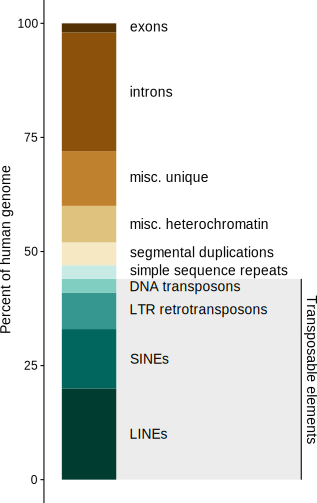
\includegraphics[width=\textwidth]{human}
  \end{minipage}
\end{figure}

The genomes of mammals, such as human, and birds exhibit much less
variation in size than, for example, the genomes of arthropods or
amphibians \citep{Gregory2005}.  In mammals, genome size varies around
five-fold and in birds even only around two-fold, whereas in insects,
the spread is around 240-fold (Figure \ref{fig:genome-size-spread},
Table \ref{tab:genome-size-spread} on page
\pageref{tab:genome-size-spread}).  This immense variation surpasses that
of amphibians, where some species have huge genomes of up to 118 Gbp,
and is paralleled only by the group of bony fishes (Osteichthyes,
excluding lungfishes), which exhibit a genome size spread of around
220-fold.  Before the discovery of TEs and non-coding DNA, such as
introns, in the genome, it was assumed that genome size should correlate
with perceived organismic complexity, but the fact that amoeba have
genomes with up to a staggering 670 Gbp \citep{Parfrey2008} did not fit
well with that assumption.  This apparent contradiction was named the
``C-value paradox'' and later renamed to ``C-value enigma''
\citep{Gregory2007}, as still a connection between genome size and
organismic complexity appears absent.

\begin{figure}
\centering
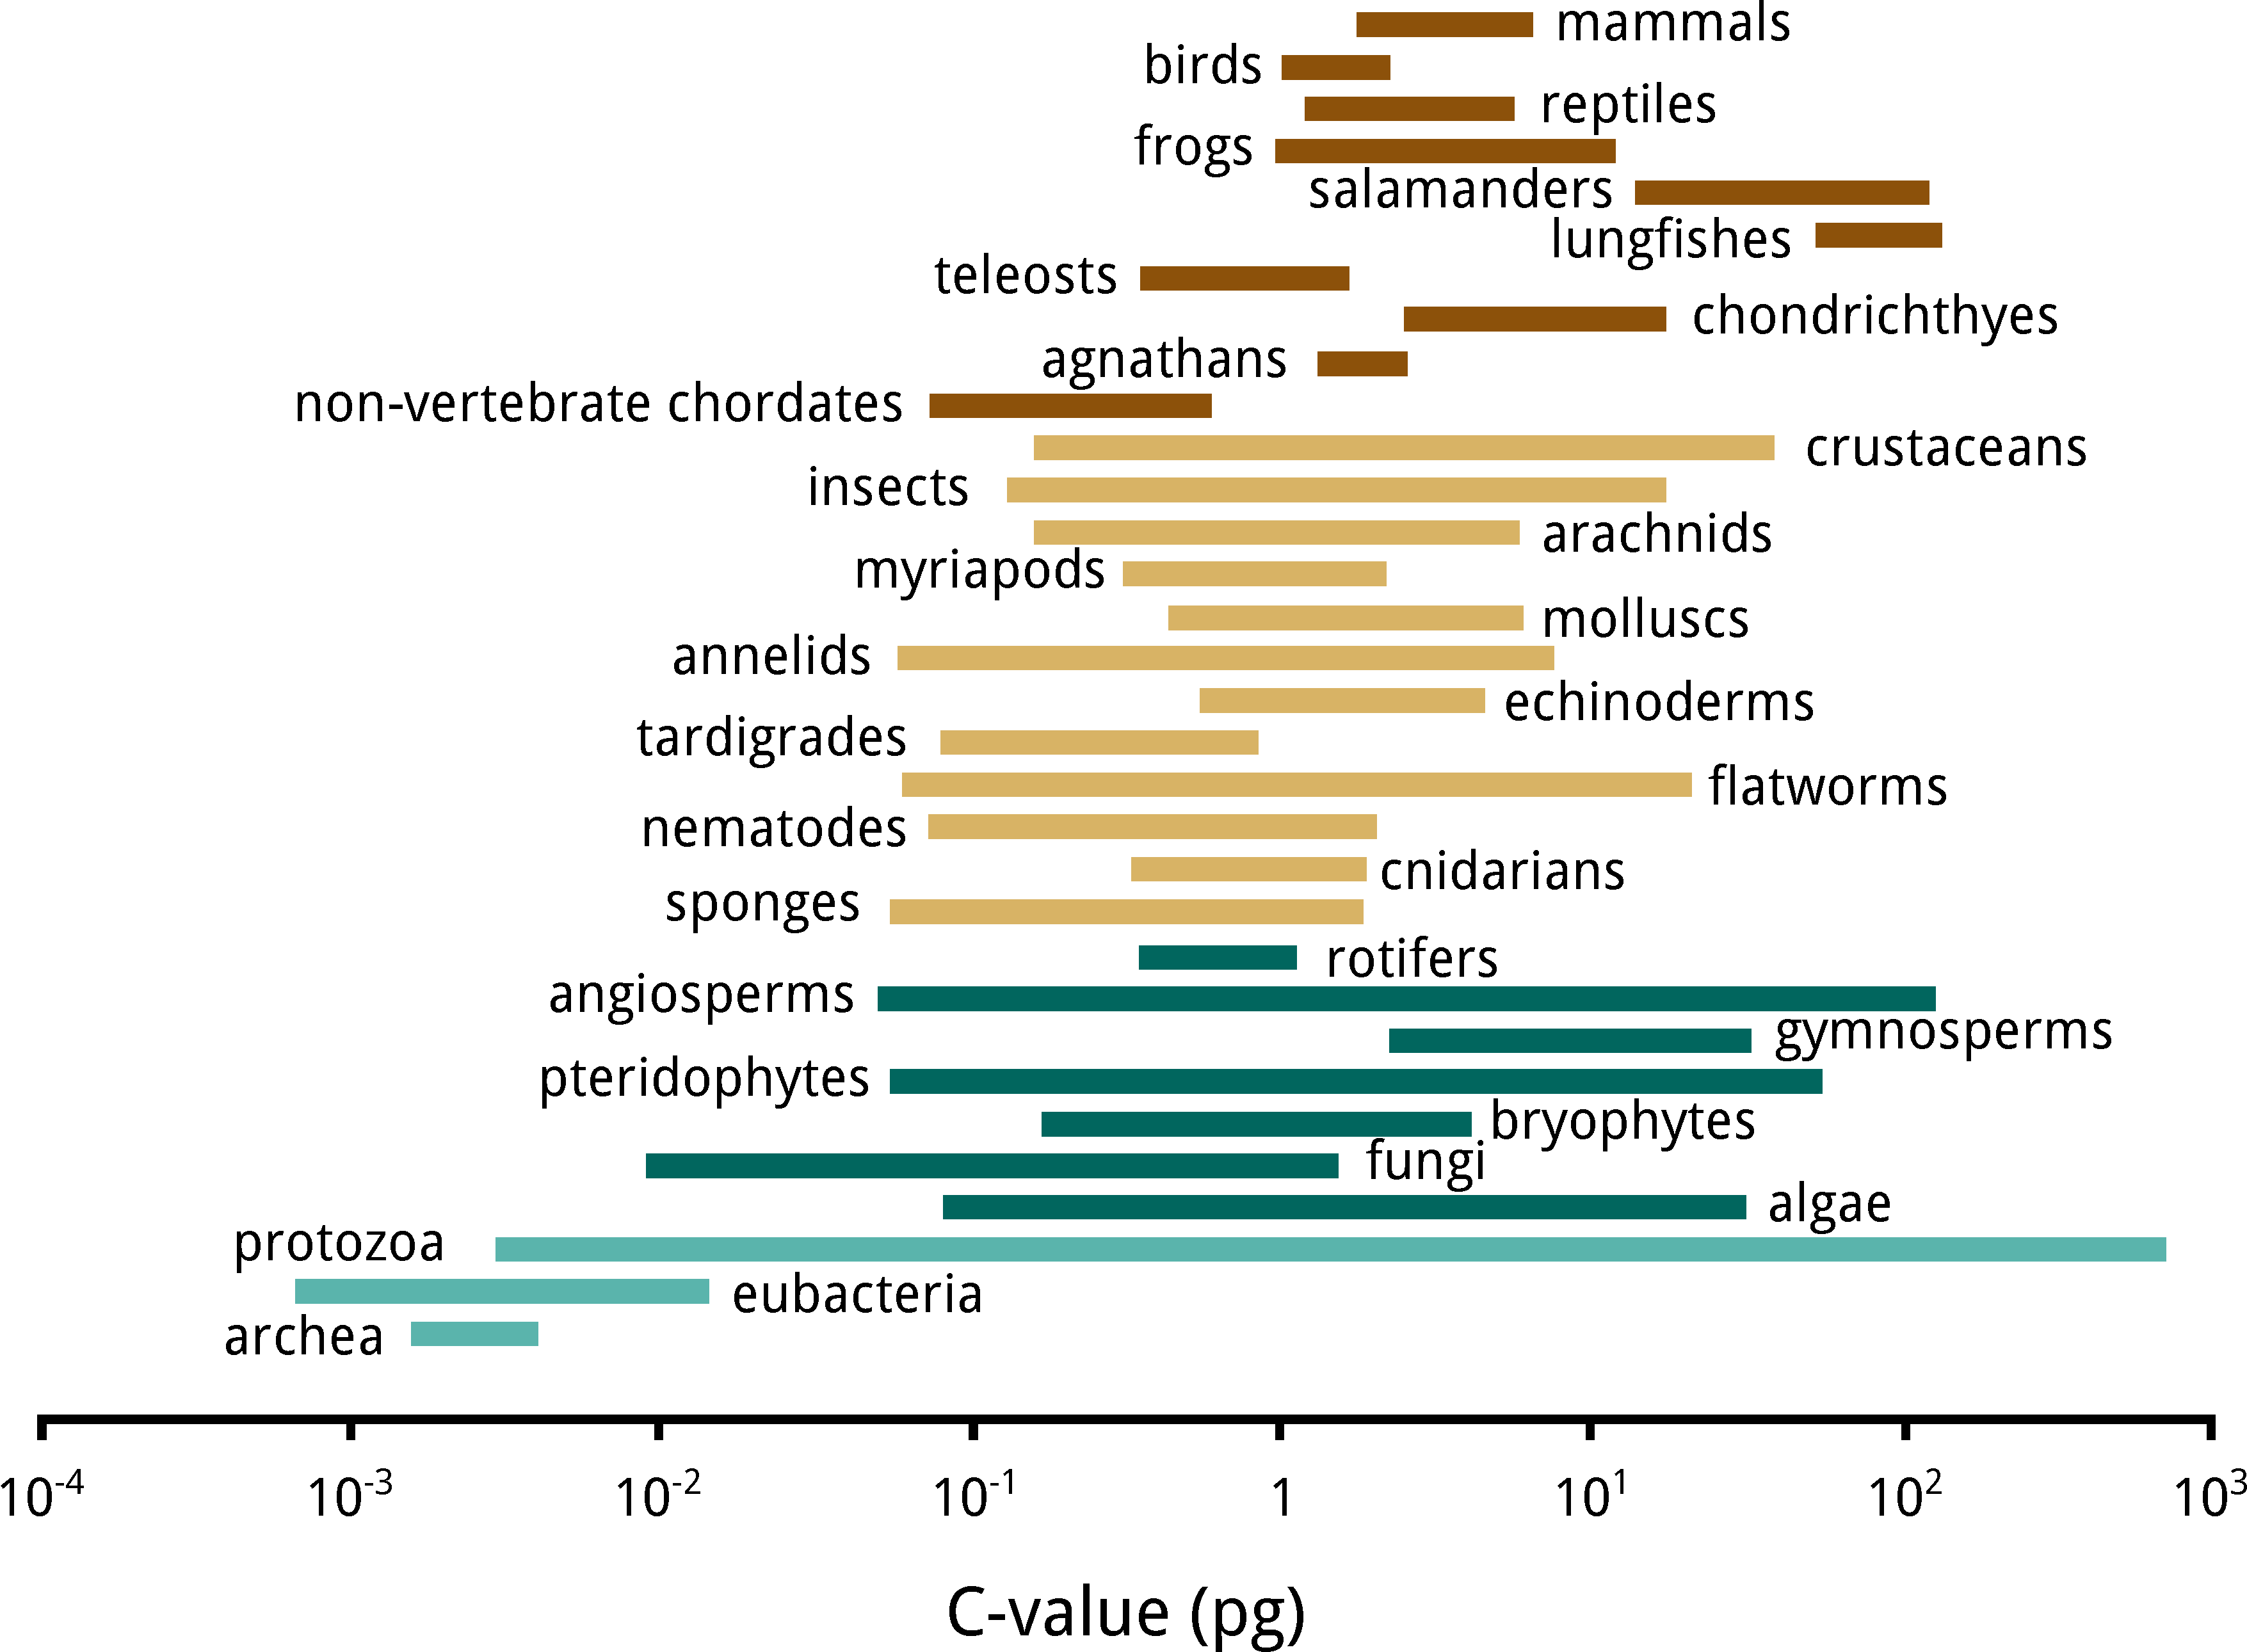
\includegraphics[width=0.7\textwidth]{genome-size-spread}
\caption[Genome size spread in eukaryotes and prokaryotes]{Genome size
spread in eukaryotes and prokaryotes.  The C-value is the amount of
haploid nuclear DNA in picogram (pg); one pg DNA is approximately 978
Mbp.  Colors are ordered for chordate animals (brown), invertebrate animals (yellow),
plants, fungi and algae (green), and prokaryotes (teal).  Figure modified from
\citet{Gregory2004}.}
\label{fig:genome-size-spread}
\end{figure}

No matter the size, the genome needs to be maintained: repair mechanisms
and transcription machinery as well as error correction use energy.  The
transcription and translation error rate increases with genome size
\citep{Zaher2009}, making more repairs necessary.  Larger genome size has
been linked to decreased development rate \citep{White2000} and
increased oxygen requirements \citep{Vinogradov1997, Gregory2002}.  In
plants \citep{Grime1983}, invertebrates \citep{Gregory2005}, and
vertebrates \citep{Horner1983, Olmo1982, Gregory2000}, it has been shown
that cell size increases with genome size \citep{Dufresne2011}.  Larger
cells are also less efficient to maintain and proliferate, and they
divide more slowly \citep{Bennett1977}.  In summary, a large genome comes
with a cost.  What would be the benefit of having a large genome?

The more genetic material in the genome, the higher the likelihood of
random mutations \citep{Wielgoss2011}.  Mutations provide the basis for
genotypic evolution: through natural selection, deleterious changes to
the genome will be removed from populations over time, and beneficial
changes --- or innovations --- prevail.  A higher mutation rate is not
always a negative property: it also brings with it a higher rate of
beneficial mutations.  Therefore, the genome is thought to reach an
equilibrium between the incurred metabolic cost of sustaining a high
mutation rate (\emph{i.e.}, the damage caused by deleterious mutations),
and the cost of mechanisms that reduce the mutation rate
\citep{Bernstein1987, Altenberg2011}.

\section{Impact of transposable elements on the genome}

The presence and activity of TEs can have disruptive influence on the
genome architecture.  By inserting at critical positions, TEs can disable
genes \citep{Kazazian1988}.  An insertion in regulatory sequence can
change gene expression \citep{Warnefors2010}.  TEs, by way of their
repetitive nature, provide hotspots for ectopic (non-homologous)
recombination \citep{Lim1988, Gray2000, Fiston-Lavier2007}, thus
increasing the likelihood for segmental duplications, deletions, and
inversions \citep{Mathiopoulos1998, Remnant2013}.  On the one hand, TEs
are obviously a source of potentially deleterious mutations.  On the
other hand, TEs can be ``domesticated'' and genes exapted from TE
sequence \citep{Gahan2001, Daborn2002, Aminetzach2005, Chen2007},
conferring novel functions to the host.  Such innovations can happen
within a few hundred generations \citep{Dolgin2006, Struchiner2009,
Kofler2015}.  As a famous example, the melanism in the British peppered
moth --- in which camouflage evolved that matches the birch trees
blackened as a result of industrialisation --- is caused by TEs
\citep{Hof2016}.  These observations document that TE activity can also
have beneficial effects on the host genome (especially in times of
stress \citep{Chenais2012}), and should therefore not be entirely
subdued.

To keep the TE population in check, defenses that remove or silence TEs
have developed in host organisms.  In many groups of organisms, a
multi-layered network of epigenetic regulation mechanisms evolved in
place to prevent TE activity at both the pre- and post-transcriptional
stage.  In plants, an epigenetic modification called DNA methylation
prevents TEs from being transcribed and thus from transposing
\citep{Slotkin2007, Lisch2009}.  After transcription, proteins from the
RNA interference (RNAi) pathway can disable messenger RNA and thereby
silence TEs \citep{Buchon2006}.  Similarly, a class of non-coding RNA,
so-called Piwi-interacting RNA (piRNA) protect the integrity of the
genome, in particular in germline cells, by forming a complex with Piwi
proteins, which can bind and cleave RNA \citep{Zeng2011}.  This complex
can recognize and silence target TEs in the RNA stage \citep{Siomi2011,
Mondal2018}.  Similar systems were identified in vertebrate genomes
\citep{Suzuki2008, Schubeler2015}: DNA methylation is thought to be a
genome defense mechanism in mammals as well \citep{Yoder1997}.
Interestingly, vertebrate genomes are globally methylated, and in plant
genomes, only gene bodies and TEs are methylated \citep{Suzuki2008}.
Fungal genomes exhibit an even more mosaic-like methylation pattern:
here, only TEs are methylated and genes are not.  In invertebrates, TEs
tend to be unmethylated.  The fruit fly \species{Drosophila melanogaster}
does not even have the methyltransferase enzyme in its gene repertoire.
Likewise, some butterfly species have lost RNAi pathway genes
\citep{Pauli2016}.  Thus, these genome defenses appear to be modular and
complementary to one another.  They are effective to a certain extent:
permanently inactive TEs become genomic ``cruft'' and are degraded by
random mutations over time and genetic drift like other parts of the
genome that are not subject to selection \citep{Szitenberg2016}.  As a
result of these extensive silencing techniques, it is not surprising
that most of the TE population in extant genomes is inactive
\citep{Yoder1997, Zilberman2007}.

There are two major models to explain TE population dynamics in the
genome: the equilibrium model and the burst model \citep{Petrov2011,
Kofler2012, Cridland2013, Blumenstiel2014}.  In the equilibrium model,
the TE insertion rate is assumed to be more or less constant, and TEs
are silenced and removed by purifying selection at a likewise constant
rate \citep{Charlesworth1983}.  This way, TE insertion rate and DNA
removal rate would cancel each other out, and the genome size remains
stable.  The equilibrium model provides a better fit for TE dynamics
under the effects of purifying selection \citep{Barron2014} than the
transposition burst model.  The burst model, which is also termed the
non-equilibrium model, predicts that TEs undergo periods of high
transposition activity while otherwise proliferating at a constant but
lower rate.  Under the transposition burst model, the absence of a
correlation between the TE age and frequency would be expected, which
better explains the observed TE age distribution in insect genomes as
well as the large genome size fluctuations during insect evolution,
given that TE abundance is a predictor for genome size
\citep{Alfsnes2017, Petersen2018a}.

\section{Insects, phylogenetics, and comparative genomics}

Insects are among the most speciose groups of organisms on earth (Figure
\ref{fig:biodiversity} on page \pageref{fig:biodiversity}) and, since
their appearance approximately 480 million years ago (Mya)
\citep{Misof2014}, have conquered land, freshwater, and air (but not
saltwater).  Protected by their hard exoskeleton, insect representatives
have invaded virtually all conceivable ecosystems including human
habitations \citep{Bertone2016}.  Insects are immensely diverse in
morphology \citep{Grimaldi2005} and often highly specialized towards a
specific food source, habitat, or lifestyle.  Bees, wasps, ants, and
termites, for example, form eusocial communities with a complex caste
system.  As disease vectors, mosquitoes are responsible for more human
deaths than all other animals combined \citep{WHO2017, Linnell2011,
Lamarque2009, DeMaddalena2008, Kasturiratne2008, Packer2005}.  Beetles,
cicadas, and grasshoppers are examples for an important source of food
for livestock and humans alike as well as a pest with high economic
impact \citep{Oliveira2014}.  Obviously, insects play pivotal roles in
most ecosystems of the planet.  Insect population diversity and
abundance, however, is declining \citep{Vogel2017} as a result of
widespread human influence (see below), with disastrous reverberations
at all levels of the local food chains.  In order to mount efficient
conservation efforts, a thorough understanding of insect biology is
required.

\begin{figure}[ht]
\centering
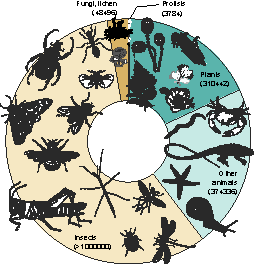
\includegraphics[width=0.9\textwidth]{biodiversity}
\caption[Biodiversity by numbers of species]
{Insects contribute more than half of the currently known species
diversity.  Data source: \citet{IUCN2018}; pictures source:
\href{https://pixabay.com}{Pixabay}, available under the Creative
Commons Public Domain license
(\href{https://creativecommons.org/publicdomain/zero/1.0}{\footnotesize{\cczero}}).}
\label{fig:biodiversity}
\end{figure}

Despite their mega-diversity and ecological importance, insects are
astonishingly understudied on the genomic level compared to other
animals: As of 2018-07-06, there were 1,115 published non-insect animal
genome sequences in the NCBI database \citep{OLeary2016} (about \p{0.3}
of the total non-insect species diversity; Figure
\ref{fig:biodiversity}) and 493 insect genomes (\p{0.065}; about five
times less genomes per species).  That number is growing by about 50
genomes per year \citep{OLeary2016}, however at this rate, it will take
more than 150 years to even sequence the genomes of \p{10} of the insect
biodiversity.  During this time, many species will have gone extinct ---
as it stands, our genome sequencing efforts are losing the race against
man-made biodiversity loss.  Ever-improving, massively parallel
sequencing technologies that appeared during the early 2000's
\citep{Behjati2013} have accelerated the pace and accuracy at which
genomes can be sequenced, but it will not be enough.  Of many insect
species, we will never be able to obtain the genomic source code, and
this will hamper our understanding of the roles these species occupied
in the interaction network of their habitats.

\label{mass-extinction}%
This not only affects insects, but all kingdoms of life: we are
currently experiencing a mass extinction event that parallels other
episodes in earth's history with high rates of biodiversity decline
\citep{Pimm1995, Dirzo2003, Schipper2008, Barnosky2011, Dirzo2014}.
Other than the five previous major extinction events
\citep{Kolbert2014}, it is anthropogenic in origin \citep{Leakey1996,
Ceballos2015} and is associated with global warming \citep{Cook2016,
Wuebbles2017}, large-scale deforestation \citep{Wright2005}, destruction
of marine and freshwater habitats \citep{Burkhead2012}, and introduction
of invasive species \citep{Mooney2001}, all hallmarks of human
influence.  Put shortly, the rate at which species go extinct is alarming
\citep{Newbold2016, Ceballos2017, Hallmann2017}, and our children will
likely experience a world with less than half the biodiversity we know
today.  While this issue has raised the attention of country leaders and
conservation policies are being put in place worldwide
\citep{Puntaru2017}, this might not be enough to reverse the trend
without sustaining irreparable damage to the ecosystems of the planet.
To make matters worse, there are signs that the issue, despite its
urgency, is fading from public awareness \citep{Kusmanoff2017}. 

We cannot save what we do not know.  Thus, conservation efforts require
intimate knowledge of the systems they aim to preserve.  The road towards
understanding the biology and the interaction of species is, however,
travelled on multiple levels.  It is not enough to observe the behaviour
or the ecology of an animal to understand the impact of it being removed
from its habitat.  It is also not enough to describe functional
morphology to gain insight on ecological implications.  Neither is it
sufficient to analyze the genes and draw conclusions based on their
composition and structure.  Profound understanding of any system can only
be gained by studying it from multiple angles and with interdisciplinary
approaches.  One approach that can add to the knowledge about a species
is to sequence and analyze its genome: the ``source code of life'' that
defines, by a manifold of means, its appearance, features, behaviour and
interactions with the environment.  By comparing the composition, the
functional networks, and other properties of one species' genome to that
of other species, one can gain insights on the mechanisms of evolution
that led to the mega-diversity of today's insects.

Comparative genomics studies --- that is, investigations comparing
genomic features of more than one species --- are not only limited by
the fact that for many species, there is no genomic sequence information
available.  Additionally, comparative analyses have to take the
evolutionary history of the species into consideration \citep{Dunn2018},
usually in the form of a phylogenetic tree that conveys information on
the species' relationships.  An undisputed phylogenetic tree down to
family level does not exist for insects so far.  \citet{Misof2014} and
the 1KITE project \citep{1KITE2018} have inferred a robust backbone
phylogeny for most major insect orders from transcriptomic data (see
below), and several publications have presented order-level phylogenies,
for example for Coleoptera \citep{McKenna2015}, Hymenoptera
\citep{Peters2017, Branstetter2017}, Lepidoptera \citep{Breinholt2018},
and Hemiptera \citep{Johnson2018}.  However, accurately reconstructing
species ancestry remains a challenge that has obstructed reliable
comparative analyses in insects so far.

Among the approaches to infer a phylogenetic species tree, the most
informed, because based on matrices with data points numbering in the
millions, is reconstruction from amino acid or nucleotide sequences.
Phylogenetic species tree reconstruction, however, regardless the
method, is no simple task and relies on sophisticated methods on all
stages of the analysis (proposed by \citet{Misof2014}, for example).
Perhaps most of all, selection of the phylogenetic markers (the features
that distinguish species and define their level of relatedness) is
paramount.   Most modern genomic studies use single-copy genes that are
found in all (or almost all) species.  The implied assumption is that
these genes share a common ancestry and are related via speciation
events, that is, they are \emph{orthologous} to one another
\citep{Koonin2005} and their phylogeny reflects the species phylogeny.

Several commonly used methods to identify orthologous genes rely on
clustering nucleotide or amino acid sequences based on their similarity
\citep{Chen2007a}.  Since orthologs tend to be more similar to each other
than to all other genes in the genomes under comparison
\citep{Altenhoff2012a}, the orthology hypothesis can be tested via a
bi-directional search for similarity applying a best reciprocal hit
(BRH) criterion: Only if the genes in question form the best search hit
in both directions (\ie, the genes are more similar to each other than
to all other genes) they can be assumed to be orthologous.  By grouping
genes from multiple species that share BRH relations, one can form
clusters of orthologous genes or simply orthologous groups (OGs)
\citep{Altenhoff2012}.  This approach has been implemented in several
software packages for use in genomic datasets \citep{Li2003,
Tatusov2003, Berglund2008, Zdobnov2017}.  Obtaining a complete and
accurate genome sequence is, however, associated with technical
difficulties and a cost that depends on the genome size.  For these
reasons, many phylogenetic studies employ transcriptomes: the nucleotide
sequences of transcripts present in the sample at the time of RNA
fixation \citep{Wang2009}.  Transcriptomes can be sequenced at a fixed
cost, however, in contrast to genomes, transcriptomes are inherently
incomplete with regard to the gene set, simply because not all genes are
expressed all the time and may therefore be absent from the sequenced
RNA sample.  While this is usually not a problem for phylogenetic
analyses \citep{Wiens2006}, it means that the above-mentioned methods to
\emph{de novo} infer orthology designed for genomes cannot not be used
on transcriptomic data.  To infer orthology among transcripts, one
usually applies a reference-based strategy that maps transcripts to
known OGs.  In the study by \citet{Misof2014}, we used a software that
implements this approach \citep{Ebersberger2009}, however, during the
analyses, it became obvious that it had several design issues that were
non-trivial to fix.  Therefore, I concepted and wrote a
re-implementation of the reference-based BRH orthology inference
approach that mitigates those issues while delivering equal performance
\citep{Petersen2017}.  The software, Orthograph, is described in chapter
\ref{cha:orthograph}.

\begin{table}
\centering\footnotesize
\caption[Genome size spread in Metazoa]{Genome size spread in Metazoa.
Values are in picogram DNA; one pg is approx. 978 mega-basepairs (Mbp).
Data from the Genome Size Database \citep{Gregory2018},
\url{http://www.genomesize.com}, accessed 2018-05-07.}
\label{tab:genome-size-spread}
\begin{tabular}{@{}lllrrrr@{}}
\toprule
Phylum     & Subphylum   & Class          & n    & min  & max   & $\Delta$fold \\
\midrule
Annelida   & --          & Oligochaeta    & 35   & 0.43 & 7.64  & 17.77  \\
Annelida   & --          & Polychaeta     & 100  & 0.06 & 7.2   & 120    \\
Arthropoda & Chelicerata & Arachnida      & 148  & 0.08 & 7.5   & 93.75  \\
Arthropoda & Crustacea   & Branchiopoda   & 68   & 0.16 & 2.91  & 18.19  \\
Arthropoda & Crustacea   & Copepoda       & 73   & 0.14 & 14.68 & 104.86 \\
Arthropoda & Crustacea   & Malacostraca   & 241  & 0.68 & 64.62 & 95.03  \\
Arthropoda & Hexapoda    & Insecta        & 1353 & 0.07 & 16.93 & 241.86 \\
Chordata   & Vertebrata  & Amphibia       & 932  & 0.95 & 120.6 & 126.95 \\
Chordata   & Vertebrata  & Aves           & 903  & 0.91 & 2.16  & 2.37   \\
Chordata   & Vertebrata  & Chondrichthyes & 199  & 1.51 & 17.05 & 11.29  \\
Chordata   & Vertebrata  & Mammalia       & 816  & 1.63 & 8.4   & 5.15   \\
Chordata   & Vertebrata  & Osteichthyes   & 1909 & 0.34 & 74.86 & 220.18 \\
Chordata   & Vertebrata  & Reptilia       & 423  & 1.05 & 5.44  & 5.18   \\
Mollusca   & --          & Bivalvia       & 108  & 0.65 & 5.4   & 8.31   \\
Mollusca   & --          & Gastropoda     & 149  & 0.43 & 7.85  & 18.26  \\
Nematoda   & --          & Secernentea    & 72   & 0.02 & 2.5   & 125    \\
\bottomrule
\end{tabular}
\end{table}

\section{Research questions}

Insects and arthropods differ at the genomic and phenotypic level from
vertebrate representatives.  Like all forms of life, they share general
mechanisms of genetic and genomic functionality and universal elements
such as genes and TEs.  However, genome composition, architecture and
structural dynamics in insects appear drastically different from
vertebrates and plants.  In particular, the insect TE repertoire has not
been subject to a large-scale study that would enable comparisons both
within and between orders.  The TE content has been assessed and put into
context with the genome size in studies focusing on mosquitoes
\citep{Neafsey2015} and \species{Drosophila} fruit flies
\citep{Sessegolo2016}), but conclusions across orders are hampered by
absent information on the TE content and composition of key species as
well as by non-standard TE annotation methods that make comparisons
difficult.  Additionally, a pan-ordinal taxon sampling could facilitate
the inference of the ancestral insect TE content. 

% hypotheses:
% a) the TE composition and abundance are not random, but
% phylogeny-dependent
% b) TE content is a predictor for genome size

In chapter \ref{cha:mobilome}, I characterize the insect TE repertoire
in a comparative standardized study based on genomic sequence data from
73 insect and non-insect arthropod species encompassing all major
orders.  The results highlight differential TE abundance and composition
in comparisons between and within insect orders.  The study also
demonstrates that the TE diversity in insects is much larger than
previously thought.  The correlation between TE content and genome size
in insects is substantiated.  Additionally, the chapter shows that the TE
copy divergence distribution is highly diverse and that some TEs are
recently active among insects.

% Warum? ``Da sind unterschiede zwischen verts und insekten, aber. . .
% weiss man noch nicht und dabei koennte . . . herauskommen''

Genome size in insects is subject to large fluctuations, and TE content
is not only correlated to genome size, but also to the insect phylogeny.
To illuminate the effects of TE activity on genome size dynamics in
insects, chapter \ref{cha:dynamics} presents an extended analysis on the
genomes of 96 arthropod species and genome size estimate data from 613
arthropod species.  The study infers a comprehensive, time-calibrated
phylogeny for these species using information from published studies and
mitochondrial nucleotide sequences.  This phylogeny is used to infer
ancestral genome sizes and the amount of genome expansion and
contraction since the last ancestor as a result of TE activity in the
genome.  It is shown that after about 100 Mya, the amount of ancestral
TEs converges to zero.  The rates of TE-associated DNA gain and loss are
correlated with the phylogeny.  The chapter also discusses a trend
towards genome size stability despite varying rates of DNA removal in
insects.

In chapter \ref{cha:orthograph}, I present the software Orthograph as a
tool for orthology assessment in transcriptomic --- or other coding
nucleotide sequence --- datasets.  Building on and incorporating existing
software packages for sequence similarity search and comparison, it
implements an algorithm that uses the BRH criterion to map transcripts
to clusters of genes with known orthology.  The software is written in a
modular fashion to make it flexible and portable.  The chapter discusses the
issues that previous implementations of the BRH mapping strategy suffer
from and shows that Orthograph overcomes them by employing a relational
database backend system that enables it to compare millions of search
results in short time.  Orthograph represents a powerful, versatile, and
future-proof application which has been used in seven co-authored
studies \citep{Mayer2016, Pauli2016, Bank2017, Dowling2017, Peters2017,
Gillung2018, Johnson2018} that are in appendix
\ref{app:papers-using-orthograph}.

Appendix \ref{app:other-publications} lists an additional seven
co-authored publications.  Among others, \citet{Misof2014} (page
\pageref{app:Misof2014}) consummates the inference of a robust
phylogenetic backbone tree of 145 insect species from all major insect
orders.  I was a major contributor to the study.  The analysis includes
node dating with a comprehensive calibration dataset of 37 fossils.  The
study presents a semi-automated and documented reproducible workflow
that facilitates phylogeny inference from transcriptomic data of many
species.  It also provides the backbone phylogeny and node dates for the
study in chapter \ref{cha:dynamics} and the breeding ground for the
development of Orthograph (chapter \ref{cha:orthograph}).

\addcontentsline{toc}{section}{References}
\bibliographystyle{apalike2}
\bibliography{references}

%!TEX root = ../dissertation.tex

\chapter{Diversity and evolution of the transposable element repertoire
in arthropods with particular reference to insects} \label{cha:mobilome}

\newpage

This chapter has been accepted for publication in \emph{BMC Evolutionary
Biology}.

\noindent \textbf{Authors:} Malte Petersen, David Armisén, Richard A. Gibbs, Lars Hering,
Abderrahman Khila, Georg Mayer, Stephen Richards, Oliver Niehuis, and
Bernhard Misof

\section{Introduction}

Repetitive elements, including transposable elements (TEs), are a major
sequence component of eukaryote genomes. In vertebrate genomes, for
example, the TE content varies from 6 \% in the pufferfish
\emph{Tetraodon nigroviridis} to more than 55 \% in the zebrafish
\emph{Danio rerio} \citep{Chalopin2015}. More than 45 \% of the human
genome \citep{deKoning2011} consist of TEs. In plants, TEs are even more
prevalent: up to 90 \% of the maize (\emph{Zea mays}) genome is covered
by TEs \citep{SanMiguel1996}. In insects, the genomic portion of TEs ranges
from as little as 1 \% in the antarctic midge \citep{Kelley2014} to as
large as 65 \% in the migratory locust \citep{Wang2014}.

TEs are known as ``jumping genes'' and traditionally viewed as selfish
parasitic nucleotide sequence elements propagating in genomes with
mainly deleterious or at least neutral effects on host fitness
\citep{Mackay1989, Pasyukova2004} (reviewed in \citet{Barron2014}). Due to their
propagation in the genome, TEs are thought to have a considerable
influence on the evolution of the host's genome architecture. By
transposing into, for example, host genes or regulatory sequences, TEs
can disrupt coding sequences or gene regulation, and/or provide hot
spots for ectopic (non-homologous) recombination that may induce
chromosomal rearrangements in the host genome such as deletions,
duplications, inversions, and translocations \citep{Burns2012}. For
example, the shrinkage of the Y chromosome in the fruit fly
\emph{Drosophila melanogaster}, which consists mostly of TEs, is thought
to be caused by such intrachromosomal rearrangements induced by ectopic
recombination \citep{Adams2000, Kent2017}. As such potent agents for mutation,
TEs are also responsible for cancer and genetic diseases in humans and
other organisms \citep{Vorechovsky2009,Chenais2015,Hancks2016}.

Despite the potential deleterious effects of their activity on gene
regulation, there is growing evidence that TEs can also be drivers of
genomic innovation that confer selective advantages to the host
\citep{Casola2007,Gonzalez2008}. For example, it is well documented that the frequent
cleavage and rearrangement of DNA strands induced by TE insertions
provides a source of sequence variation to the host genome, or that by a
process called molecular domestication of TEs, host genomes derive new
functional genes and regulatory networks \citep{Feschotte2008,Bohne2008,Santos2014}.
Furthermore, many exons have been \emph{de novo}-recruited from TE
insertions in coding sequences of the human genome \citep{Zhang2006}.
In insects, TE insertions have played a pivotal role in the acquisition
of insecticide resistance \citep{Chen2007,Itokawa2010,Gahan2001}, as well as in the rewiring
of a regulatory network that provides dosage compensation
\citep{Ellison2013}, or the evolution of climate adaptation
\citep{Gonzalez2010,Kim2014}.

TEs are classified depending on their mode of transposition. Class I
TEs, also known as retrotransposons, transpose via an RNA-mediated
mechanism that can be circumscribed as ``copy-and-paste''. They are
further subdivided into long terminal repeat (LTR) retrotransposons and
non-LTR retrotransposons. Non-LTR retrotransposons include long and
short interspersed nuclear elements (LINEs and SINEs)
\citep{Malik1999,Eickbush2008}. Whereas LTR retrotransposons and LINEs encode a
reverse transcriptase, the non-autonomous SINEs rely on the
transcriptional machinery of autonomous elements, such as LINEs, for
mobility. Frequently found LTR retrotransposon families in eukaryote
genomes include Ty3/Gypsy, which was originally described in
\emph{Arabidopsis thaliana} \citep{Marin2000}, Ty1/Copia
\citep{Flavell1992}, as well as BEL/Pao \citep{delaChaux2011}.

In Class II TEs, also termed DNA transposons, the transposition is
DNA-based and does not require an RNA intermediate. Autonomous DNA
transposons encode a transposase enzyme and move via a ``cut-and-paste''
mechanism. During replication, terminal inverted repeat (TIR)
transposons and Crypton-type elements cleave both DNA strands
\citep{Wicker2007}. Helitrons, also known as rolling-circle (RC)
transposons due to their characteristic mode of transposition
\citep{Kapitonov2001}, and the self-synthesizing Maverick/Polinton elements
\citep{Krupovic2016} cleave a single DNA strand in the process of
replication. Both Helitron and Maverick/Polinton elements occur in
autonomous and non-autonomous versions \citep{Kapitonov2006,Kapitonov2007}, the latter of
which do not encode all proteins necessary for transposition. Helitrons
are the only Class II transposons that do not cause a flanking target
site duplication when they transpose. Class II also encompasses other
non-autonomous DNA transposons such as miniature inverted TEs (MITEs)
\citep{Shirasawa2012}, which exploit and rely on the transposase mechanisms
of autonomous DNA transposons to replicate.

Previous reports on insect genomes describe the composition of TE
families in insect genomes as a mixture of insect specific TEs and TEs
common to metazoa \citep{Feschotte2007,Maumus2015,Chuong2016}. Overall, surprisingly little
effort has been put into characterizing TE sequence families and TE
compositions in insect genomes in large-scale comparative analyses
encompassing multiple taxonomic orders to paint a picture of the insect
TE repertoire. Dedicated comparative analyses of TE composition have
been conducted on species of mosquitoes \citep{Neafsey2015}, of
drosophilid flies \citep{Sessegolo2016}, and of \emph{Macrosiphini}
(aphids) \citep{Bouallegue2017}. Despite these efforts in characterizing TEs
in insect genomes, still little is known about the diversity of TEs in
insect genomes, owed in part to the huge insect species diversity and to
the lack of a standardized analysis that allows comparisons across
taxonomic orders. While this lack of knowledge is due to the low
availability of sequenced insect genomes in the past, efforts such as
the i5k initiative \citep{Robinson2011} have helped to increase the number
of genome sequences from previously unsampled insect taxa. With this
denser sampling of insect genomic diversity available, it now seems
possible to comprehensively investigate the TE diversity among major
insect lineages.

Here, we present the first exhaustive analysis of the distribution of TE
classes in a sample representing half of the currently classified insect
(hexapod \emph{sensu} Misof \emph{et al.} \citep{Misof2014}) orders and
using standardized comparative methods implemented in recently developed
software packages. Our results show similarities in TE family diversity
and abundance among the investigated insect genomes, but also profound
differences in TE activity even among closely related species.


\section{Materials and methods}

\subsection{Genomic data sets}

We downloaded genome assemblies of 42 arthropod species from NCBI
GenBank at \url{ftp.ncbi.nlm.nih.gov/genomes} (last accessed 2014-11-26;
supplementary table \ref{tab:urls}) as well as the genome assemblies of 31
additional species from the i5k FTP server at
\href{ftp://ftp.hgsc.bcm.edu:/I5K-pilot/}{ftp.hgsc.bcm.edu/I5K-pilot}
(last accessed 2016-07-08; supplementary table \ref{tab:urls}). Our taxon sampling
includes 21 dipterans, four lepidopterans, one trichopteran, five
coleopterans, one strepsipteran, 14 hymenopterans, one psocodean, six
hemipterans, one thysanopteran, one blattodean, one isopteran, one
orthopteran, one ephemeropteran, one odonate, one archaeognathan, and
one dipluran. As outgroups we included three crustaceans, one myriapod,
six chelicerates, and one onychophoran.

\subsection{Construction of species-specific repeat libraries and TE
annotation in the genomes}

We compiled species-specific TE libraries using automated annotation
methods. RepeatModeler Open-1.0.8 \citep{Smit2015} was employed to
cluster repetitive \emph{k}-mers in the assembled genomes and infer
consensus sequences. These consensus sequences were classified using a
reference-based similarity search in RepBase Update 20140131
\citep{Jurka2005}. The entries in the resulting repeat libraries were
then searched for using nucleotide BLAST in the NCBI nr database
(downloaded 2016-03-17 from
\href{ftp://ftp.ncbi.nlm.nih.gov/blast/db}{ftp.ncbi.nlm.nih.gov/blast/db})
to verify that the included consensus sequences are indeed TEs and not
annotation artifacts. Repeat sequences that were annotated as
``unknown'' and that resulted in a BLAST hit for known TE proteins such
as reverse transcriptase, transposase, integrase, or known TE domains
such as gag/pol/env, were kept and considered unknown TE nucleotide
sequences; but all other ``unknown'' sequences were not considered TE
sequences and therefore removed. The filter patterns are included in the data
package available at the Dryad repository at the URI~\url{https://doi.org/10.5061/dryad.55p667b}. The filtered repeat library was combined with the
Metazoa-specific section of RepBase version 20140131 and subsequently used with
RepeatMasker 4.0.5 \citep{Smit2015} to annotate TEs in the genome assemblies.

\subsection{Validation of Alu
presence}

To exemplarily validate our annotation, we selected the SINE Alu, which
was previously only identified in primates \citep{Kriegs2007}. We
retrieved a Hidden Markov model (HMM) profile for the AluJo subfamily
from the repeat database Dfam \citep{Hubley2015} and used the HMM to
search for Alu copies in the genome assemblies. We extracted the hit
nucleotide subsequences from the assemblies and inferred a multiple
nucleotide sequence alignment with the canonical Alu nucleotide sequence
from Repbase \citep{Jurka2005}.

\subsection{Genomic TE coverage and correlation with genome
size}

We used the tool ``one code to find them all'' \citep{Bailly-Bechet2014} on the
RepeatMasker output tables to calculate the genomic proportion of
annotated TEs. ``One code to find them all'' is able to merge entries
belonging to fragmented TE copies to produce a more accurate estimate of
the genomic TE content and especially the copy numbers. To test for a
relationship between genome assembly size and TE content, we applied a
linear regression model and tested for correlation using the Spearman
rank sum method. To see whether the genomes of holometabolous insects
are different than the genomes of hemimetabolous insects in TE content,
we tested for an effect of the taxa using their mode of metamorphosis as
a three-class factor: Holometabola (all holometabolous insect species),
non-Eumetabola (all non-holometabolous hexapod species, with the
exception of Hemiptera, Thysanoptera, and Psocodea; \citep{Beutel2013}),
and Acercaria (Hemiptera, Thysanoptera, and Psocodea). We also tested
for a potential phylogenetic effect on the correlation between genome
size and TE content with the phylogenetic independent contrasts (PIC)
method proposed by Felsenstein \citep{Felsenstein1985} using the ape package
\citep{Paradis2004} within R \citep{RCoreTeam2017}





\subsection{Kimura distance-based TE age
distribution}

We used intra-family TE nucleotide sequence divergence as a proxy for
intra-family TE age distributions. Sequence divergence was calculated as
intra-family Kimura distances (rates of transitions and transversions)
using the specialized helper scripts from the RepeatMasker 4.0.5
package. The tools compute the Kimura distance between each annotated TE
copy and the consensus sequence of the respective TE family, and provide
the data in tabular format for processing. When plotted (Fig. \ref{fig:landscapes}), a peak
in the distribution shows the genomic coverage of the TE copies with
that specific Kimura distance to the repeat family consensus. Thus, a
large peak with high Kimura distance would indicate a group of TE copies
with high sequence divergence due to genetic drift or other processes.
The respective TE copies are likely older than copies associated with a
peak at low Kimura distance. We used the Kimura distances without
correction for CpG pairs since TE DNA methylation is clearly absent in
holometabolous insects and insufficiently described in hemimetabolous
insects \citep{Glastad2014}. All TE age distribution landscapes were
inferred from the data obtained by annotating the genomes with \emph{de
novo}-generated species-specific repeat libraries.

\section{Results}

\subsection{Diversity of TE content in arthropod
genomes}

TE content varies greatly among the analyzed species (Fig. \ref{fig:te-coverage},
supplemental table \ref{tab:coverage}) and differs even between species belonging the
same order. In the insect order Diptera, for example, the TE content
varies from around 55 \% in the yellow fever mosquito \emph{Aedes
aegypti} to less than 1 \% in \emph{Belgica antarctica}. Even among
closely related \emph{Drosophila} species, the TE content ranges from 40
\% (in \emph{D. ananassae}) to 10 \% (in \emph{D. miranda} and \emph{D.
simulans}). The highest TE content (60 \%) was found in the large genome
(6.5 Gbp) of the migratory locust \emph{Locusta migratoria}
(Orthoptera), while the smallest known insect genome, that of the
antarctic midge \emph{B. antarctica} (Diptera, 99 Mbp), was found to
contain less than 1 \% TEs. The TE content of the majority of the
genomes was spread around a median of 24.4 \% with a standard deviation
of 12.5 \%.

\begin{figure}[h!]
\begin{center}
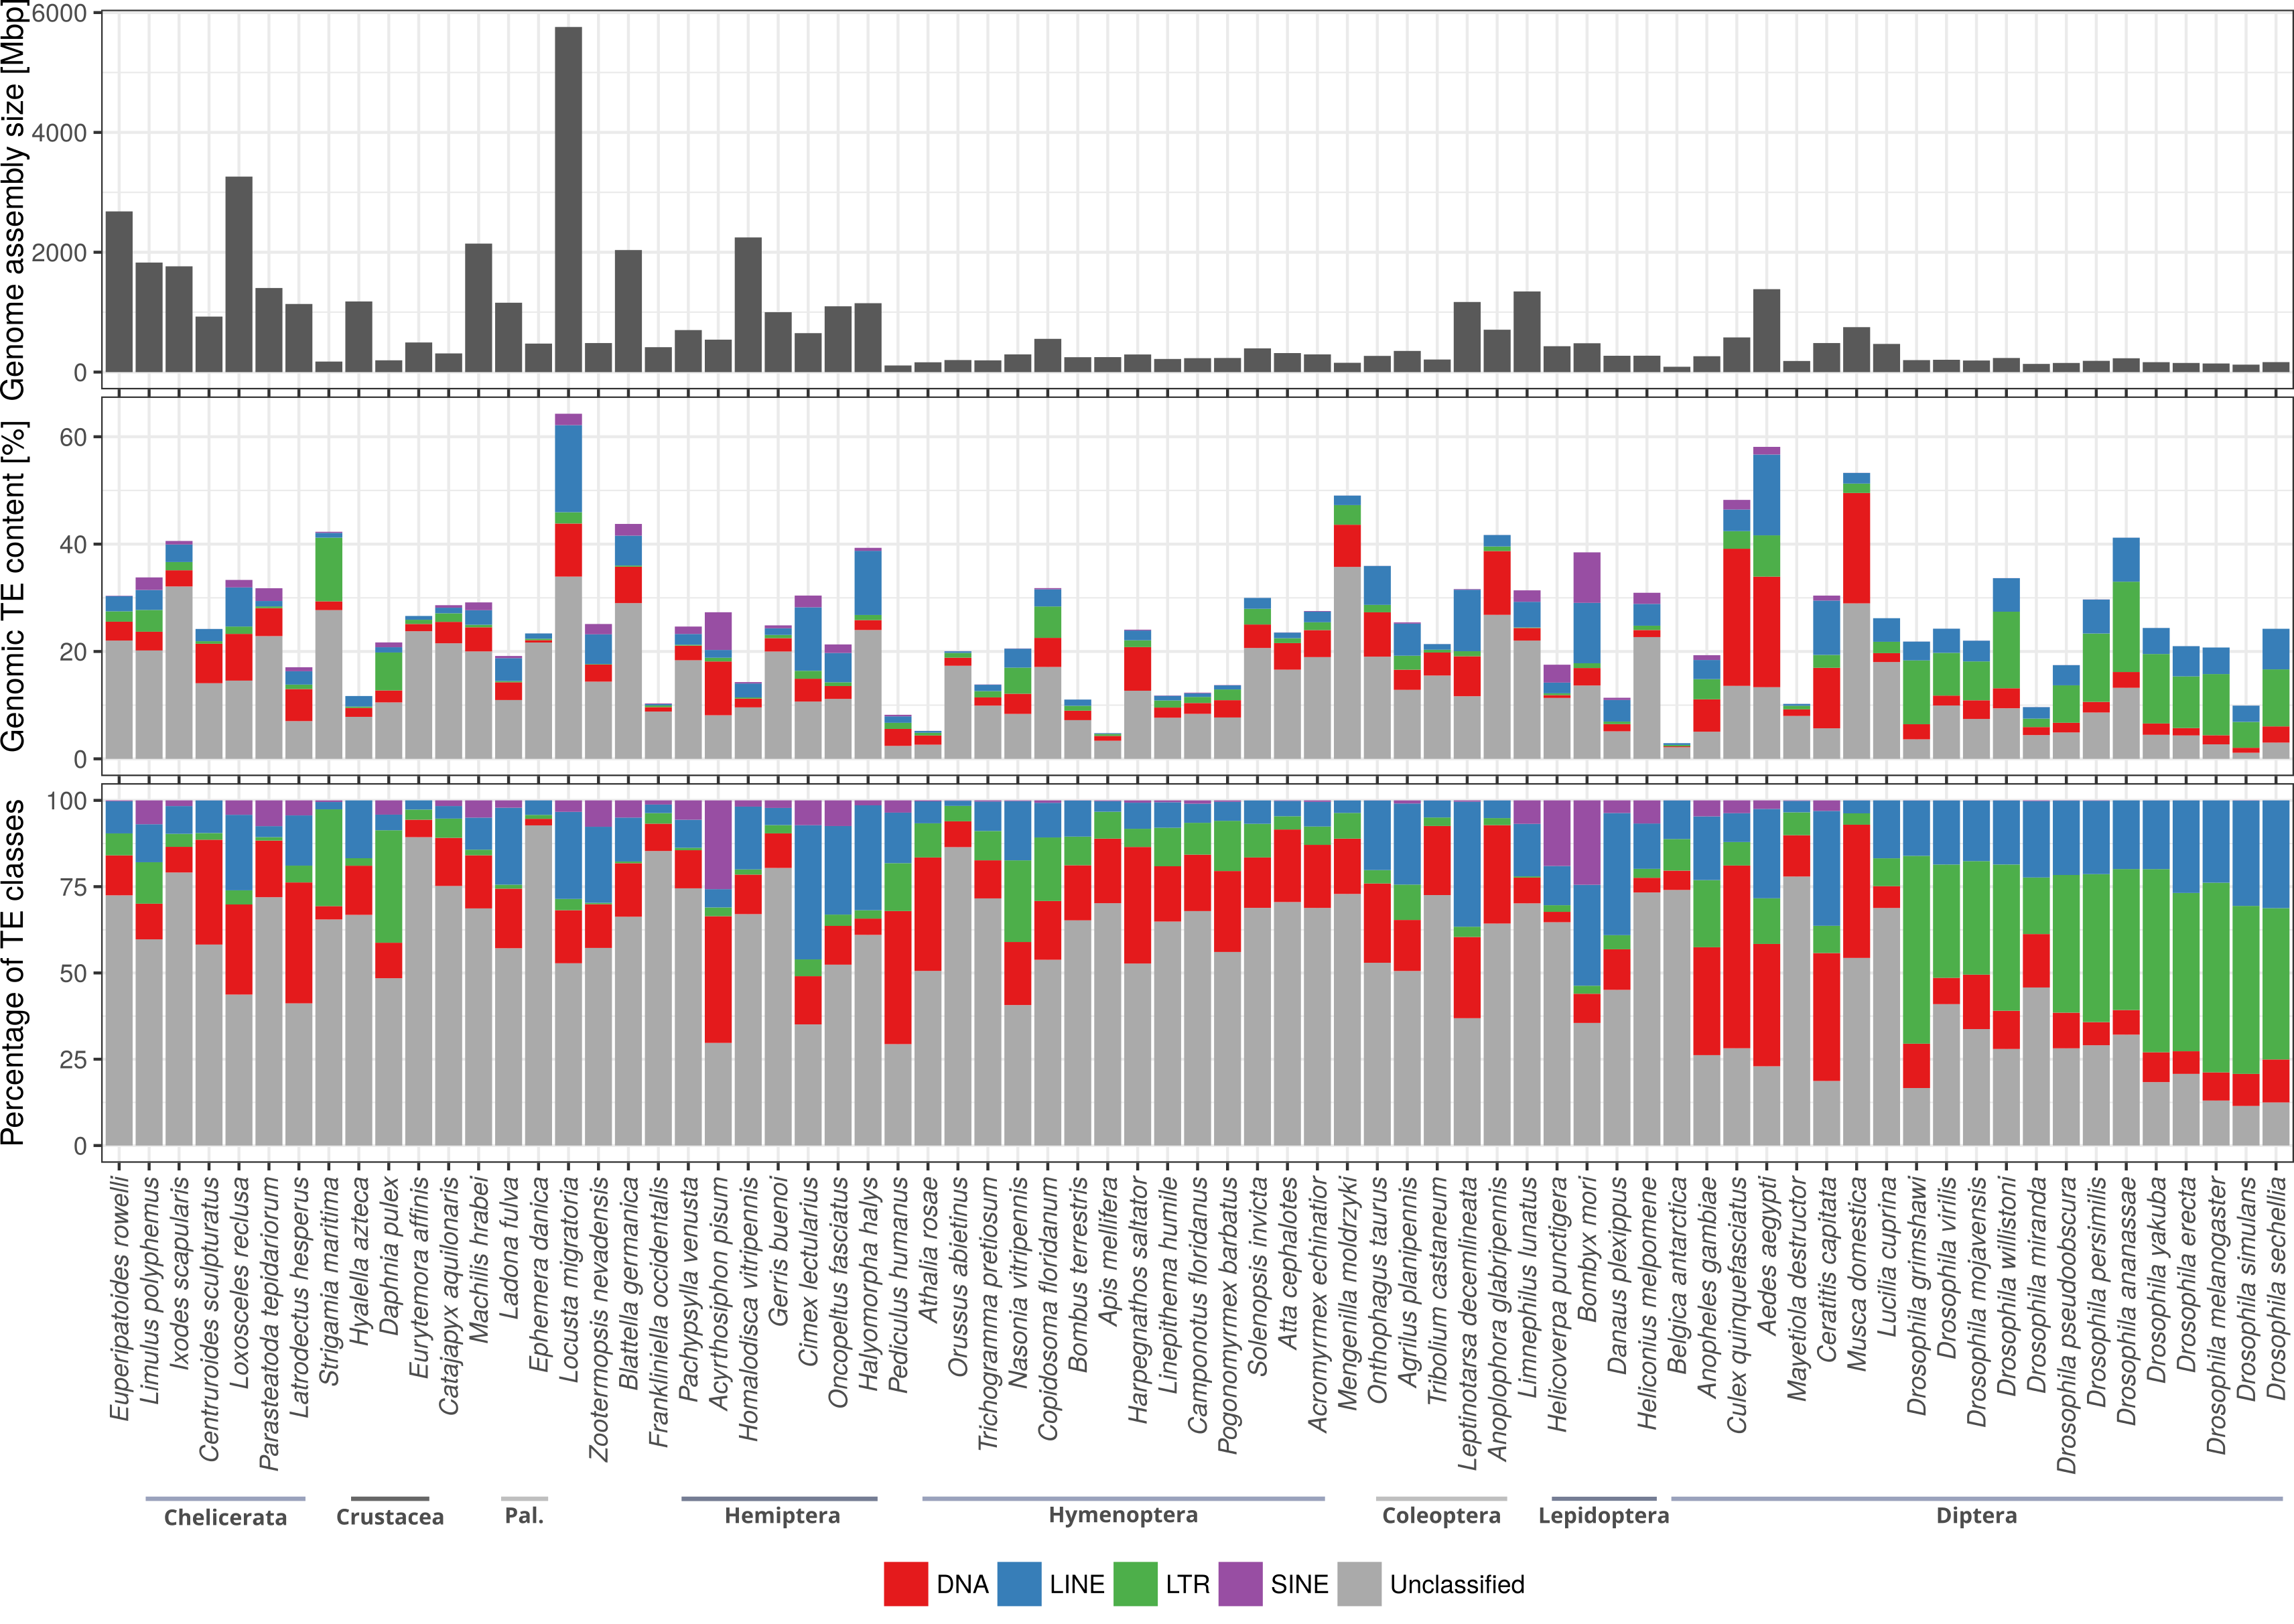
\includegraphics[width=\textwidth]{te-coverage-in-insect-genomes-both}
\caption[Arthropod genome size and TE coverage]{{Genome assembly size, total amount and relative proportion of DNA
transposons, LTR, LINE and SINE retrotransposons in arthropod genomes
and a representative of Onychophora as an outgroup. Also shown is the
genomic proportion of unclassified/uncharacterized repetitive elements.
Pal., Palaeoptera%
\label{fig:te-coverage}
}}
\end{center}
\end{figure}

\subsection{Relative contribution of different TE types to arthropod
genome
sequences}

We assessed the relative contribution of the major TE groups (LTR, LINE,
SINE retrotransposons, and DNA transposons) to the arthropod genome
composition (Fig. \ref{fig:te-coverage}). In most species, ``unclassified'' elements, which
need further characterization, represent the largest fraction. They
contribute up to 93 \% of the total TE coverage in the mayfly
\emph{Ephemera danica} or the copepod \emph{Eurytemora affinis}.
Unsurprisingly, in most investigated \emph{Drosophila} species the
unclassifiable elements comprise less than 25 \% and in \emph{D.
simulans} only 11 \% of the entire TE content, likely because the
\emph{Drosophila} genomes are well annotated and most of their content
is known (in fact, many TEs were first found in representatives of
\emph{Drosophila}). Disregarding these unclassified TE sequences, LTR
retrotransposons dominate the TE content in representatives of Diptera,
in some cases contributing around 50 \% (e.g., in \emph{D. simulans}).
In Hymenoptera, on the other hand, DNA transposons are more prevalent,
such as 35.25 \% in Jerdon's jumping ant \emph{Harpegnathos saltator}.
LINE retrotransposons are represented with up to 39.3 \% in Hemiptera
and Psocodea (\emph{Acyrthosiphon pisum} and \emph{Cimex lectularius}),
with the exception of the human body louse \emph{Pediculus humanus},
where DNA transposons contribute 44.43 \% of the known TE content. SINE
retrotransposons were found in all insect orders, but they contributed
less than 10 \% of the genomic TE content in any taxon in our sampling,
with the exception of \emph{Helicoverpa punctigera} (18.48 \%),
\emph{Bombyx mori} (26.38 \%), and \emph{A. pisum} (27.11 \%). In some
lineages, such as Hymenoptera and most dipterans, SINEs contribute less
than 1 \% to the TE content, whereas in Hemiptera and Lepidoptera the
SINE coverage ranges from 0.08 \% to 26.38 \% (Hemiptera) and 3.35 \% to
26.38 \% (Lepidoptera). Note that these numbers are likely higher and
many more DNA, LTR, LINE, and SINE elements may be obscured by the large
``unclassified'' portion.

\subsection{Contribution of TEs to arthropod genome
size}

We assessed the TE content, that is, the ratio of TE versus non-TE
nucleotides in the genome assembly, in 62 hexapod (insects \emph{sensu}
\citep{Misof2014}) species as well as an outgroup of 10 non-insect
arthropods and a representative of Onychophora (velvet worms). We tested
whether there was a relationship between TE content and genome assembly
size, and found a positive correlation (Fig. \ref{fig:te-coverage-vs-genome-size} and supplemental table
\ref{tab:coverage}). This correlation is statistically significant (Spearman's rank sum
test, \(\rho = 0.495\), \(p \lll 0.005\)). Genome size is significantly
smaller in holometabolous insects than in non-holometabolous insects
(one-way ANOVA, \(p = 0.0001\)). Using the \texttt{ape} package v. 4.1
\citep{Paradis2004} for R \citep{RCoreTeam2017}, we tested for correlation
between TE content and genome size using phylogenetically independent
contrasts (PIC) \citep{Felsenstein1985}. The test confirmed a significant
positive correlation (Pearson product-moment correlation,
\(\rho = 0.497\), \(p = 0.0001\), corrected for phylogeny using PIC)
between TE content and genome size. Additionally, genome size is
correlated with TE diversity, that is, the number of different TE
superfamilies found in a genome (Spearman, \(\rho = 0.712\),
\(p \lll 0.005\)); this is also true under PIC (Pearson,
\(\rho = 0.527\), \(p \lll 0.005\); Fig. \ref{fig:te-families-vs-genome-size}).

\begin{figure}[h!]
\begin{center}
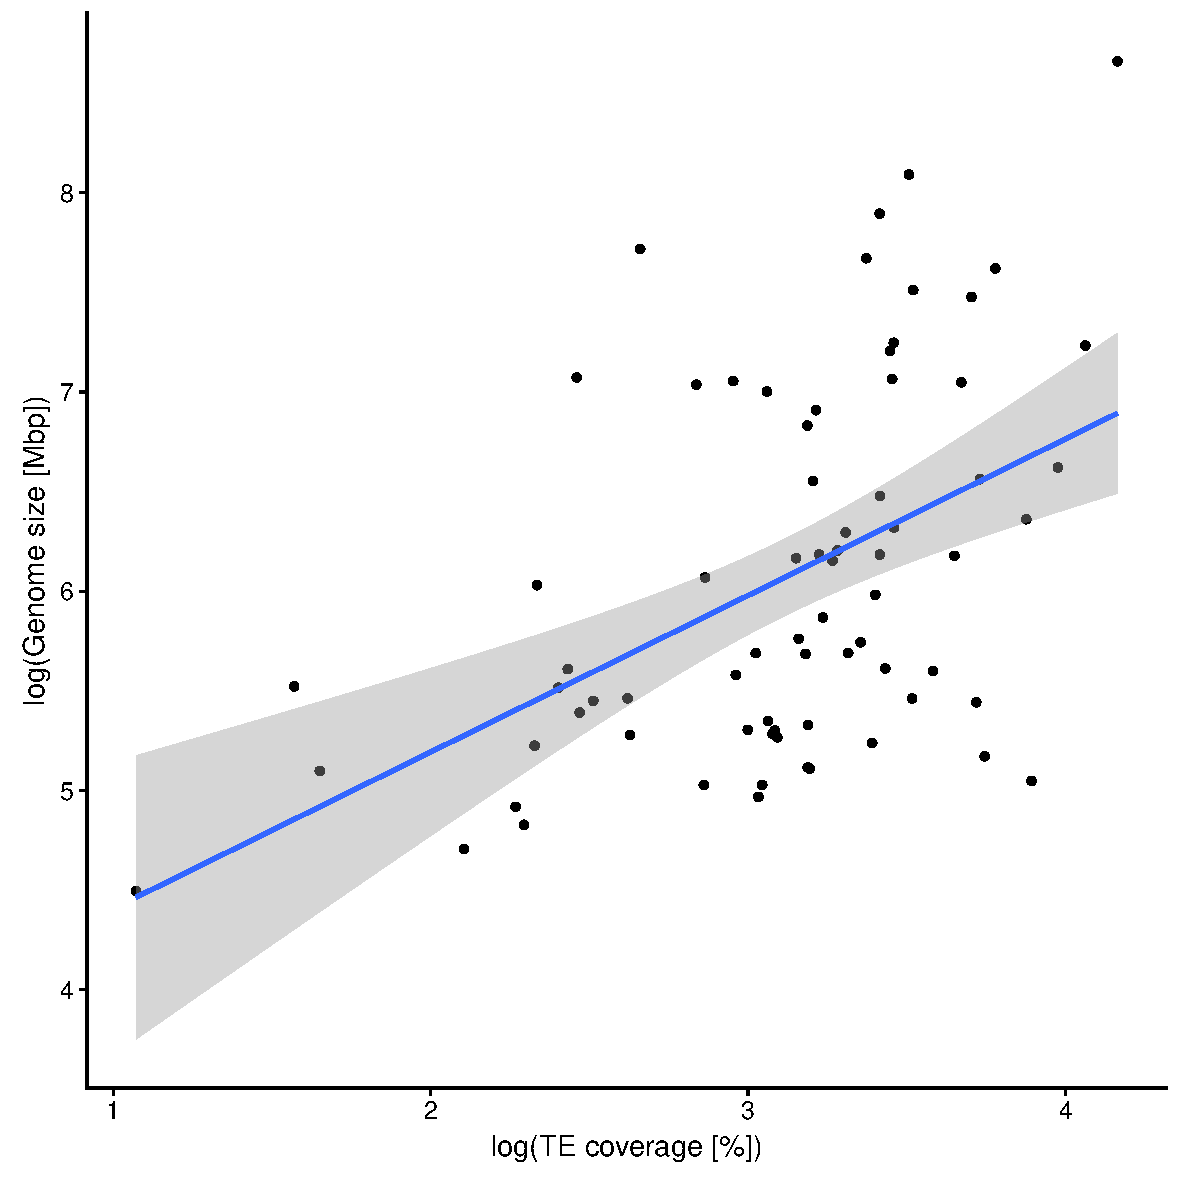
\includegraphics[width=\textwidth]{te-coverage-vs-genome-size}
\caption[TE content is positively correlated to genome size in arthropods]{{TE content in 73 arthropod genomes is positively correlated to genome
assembly size (Spearman rank correlation test, \(\rho = 0.495\),
\(p \lll 0.005\)). This correlation is also supported under
phylogenetically independent contrasts \protect\citep{Felsenstein1985} (Pearson
product moment correlation, \(\rho = 0.497\), \(p = 0.0001225\)). Dots:
Individual measurements; blue line: linear regression; grey area:
confidence interval.%
\label{fig:te-coverage-vs-genome-size}
}}
\end{center}
\end{figure}

\subsection{Distribution of TE superfamilies in
arthropods}

We identified almost all known TE superfamilies in at least one insect
species, and many were found to be widespread and present in all
investigated species (Fig. \ref{fig:presence-absence}, note that in this figure, TE families were
summarized in superfamilies). Especially diverse and ubiquitous are DNA
transposon superfamilies, which represent 22 out of 70 identified TE
superfamilies. The most widespread (present in all investigated species)
DNA transposons belong to the superfamilies Academ, Chapaev and other
superfamilies in the CMC complex, Crypton, Dada, Ginger, hAT (Blackjack,
Charlie, \emph{etc.}), Kolobok, Maverick, Harbinger, PiggyBac, Helitron
(RC), Sola, TcMar (Mariner, Tigger, \emph{etc.}), and the P element
superfamily. LINE non-LTR retrotransposons are similarly ubiquitous,
though not as diverse. Among the most widespread LINEs are TEs belonging
to the superfamilies CR1, Jockey, L1, L2, LOA, Penelope, R1, R2, and
RTE. Of the LTR retrotransposons, the most widespread are in the
superfamilies Copia, DIRS, Gypsy, Ngaro, and Pao as well as endogenous
retrovirus particles (ERV). SINE elements are diverse, but show a more
patchy distribution, with only the tRNA-derived superfamily present in
all investigated species. We found elements belonging to the ID
superfamily in almost all species except the Asian long horned beetle,
\emph{Anoplophora glabripennis}, and the B4 element absent from eight
species. All other SINE superfamilies are absent in at least 13 species.
Elements from the Alu superfamily were found in 48 arthropod genomes,
for example in the silkworm \emph{Bombyx mori} (Fig. \ref{fig:alu-alignment}, all Alu
alignments are shown in Additional File 1).

\begin{figure}[h!]
\begin{center}
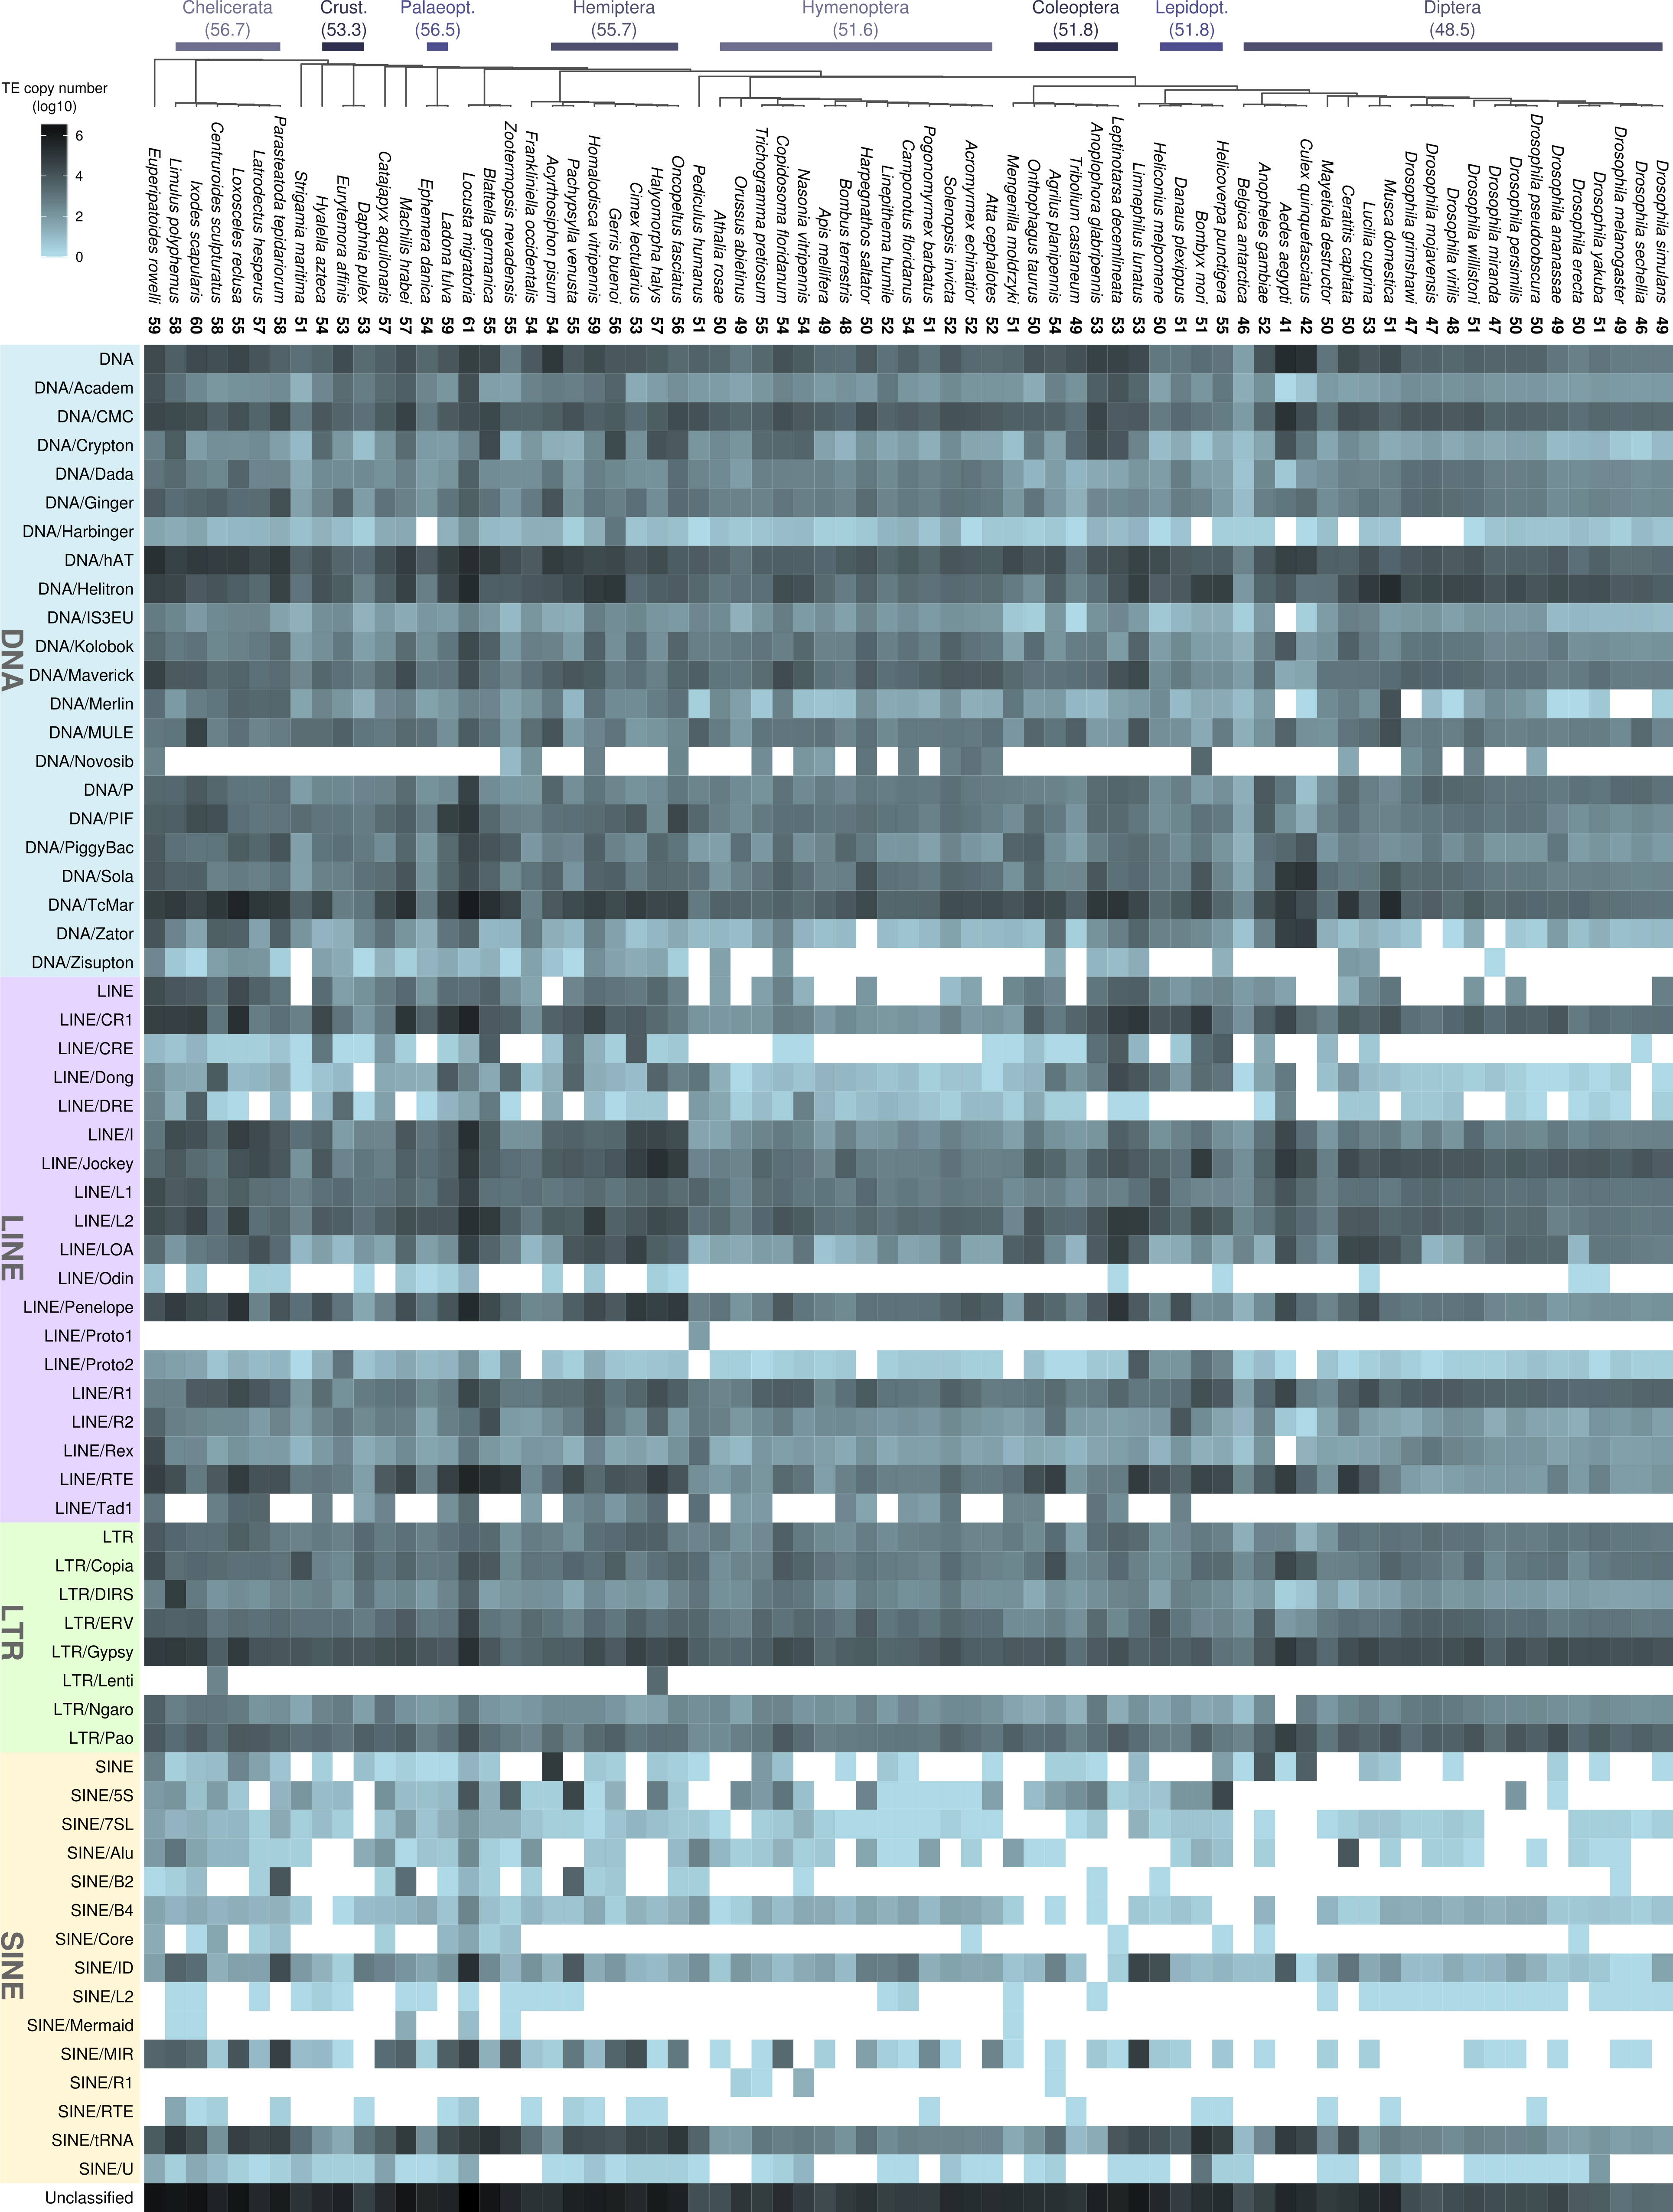
\includegraphics[width=\textwidth]{presence-absence-reduced-with-tree}
\caption[TE superfamily diversity in arthropod genomes]{{TE diversity in arthropod genomes: Many known TE superfamilies were
identified in almost all insect species. Presence of TE superfamilies is
shown as filled cells with the color gradient showing the TE copy number
(log11). Empty cells represent absence of TE superfamilies. The numbers
after each species name show the number of different TE superfamilies;
numbers in parentheses below clade names denote the average number of TE
superfamilies in the corresponding taxon.%
\label{fig:presence-absence}
}}
\end{center}
\end{figure}

\begin{figure}[h!]
\begin{center}
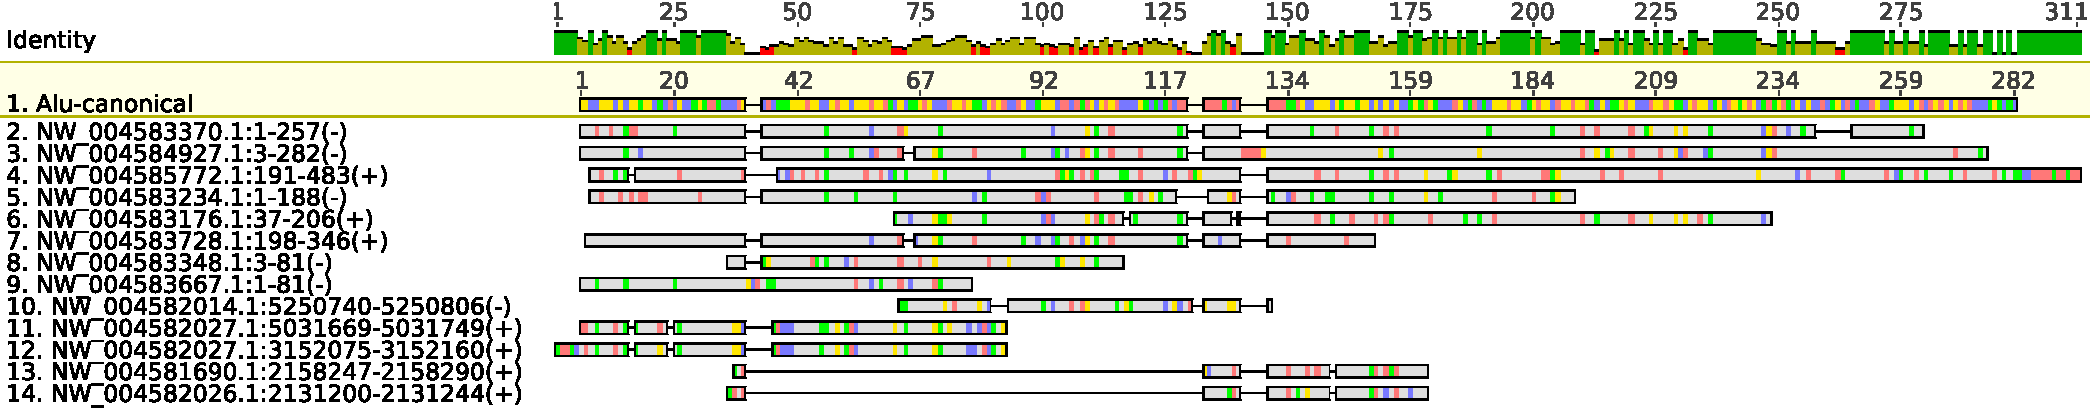
\includegraphics[width=\textwidth]{Alu-in-Zootermopsis-nevadensis}
\caption[The Alu element found in the \emph{Bombyx mori} genome]{{The Alu element found in~\emph{Bombyx mori}: Alignment of the canonical
Alu sequence from Repbase with HMM hits in the~\emph{B. mori} genome
assembly. Grey areas in the sequences are identical to the canonical Alu
sequence. The sequence names follow the pattern
``identifier:start-end(strand)'' Image created using Geneious version
7.1 created by Biomatters. Available
from \url{https://www.geneious.com}
{\label{fig:alu-alignment}}%
}}
\end{center}
\end{figure}

On average, the analyzed species harbor a mean of 54.8 different TE
superfamilies, with the locust \emph{L. migratoria} exhibiting the
greatest diversity (61 different TE superfamilies), followed by the tick
\emph{Ixodes scapularis} (60), the velvet worm \emph{Euperipatoides
rowelli} (59), and the dragonfly \emph{Ladona fulva} (59). Overall,
Chelicerata have the highest average TE superfamily diversity (56.7).
The greatest diversity among the multi-representative hexapod orders was
found in Hemiptera (55.7). The mega-diverse insect orders Diptera,
Hymenoptera, and Coleoptera display a relatively low diversity of TE
superfamilies (48.5, 51.8, and 51.8, respectively). The lowest diversity
was found in \emph{A. aegypti}, with only 41 TE superfamilies.

\subsection{Lineage-specific TE presence and absence in insect
orders}

We found lineage-specific TE diversity within most insect orders. For
example, the LINE superfamily Odin is absent in all Hymenoptera studied,
whereas Proto2 was found in all Hymenoptera except in the ant \emph{H.
saltator} and in all Diptera except in \emph{C. quinquefasciatus}.
Similarly, the Harbinger DNA element superfamily was found in all
Lepidoptera except for the silkworm \emph{B. mori}. Also within
Palaeoptera (\emph{i.e.}, mayflies, damselflies, and dragonflies), the
Harbinger superfamily is absent in \emph{E. danica}, but present in all
other representatives of Palaeoptera. These clade-specific absences of a
TE superfamily may be the result of lineage-specific TE extinction
events during the evolution of the different insect orders. Note that
since a superfamily can encompass multiple different TEs, the absence of
a specific superfamily can either result from independent losses of
multiple TEs belonging to that superfamily, or a single loss if there
only was a single TE of that superfamily in the genome.

We also found TE superfamilies represented only in a single species of
an insect clade. For example, the DNA element superfamily Zisupton was
found only in the wasp \emph{Copidosoma floridanum}, but not in other
Hymenoptera, and the DNA element Novosib was found only in \emph{B.
mori}, but not in other Lepidoptera. Within Coleoptera, only the
Colorado potato beetle, \emph{Leptinotarsa decemlineata} harbors the
LINE superfamily Odin. Likewise, we found the Odin superfamily among
Lepidoptera only in the noctuid \emph{Helicoverpa punctigera}. We found
the LINE superfamily Proto1 only in \emph{Pediculus humanus} and in no
other species. These examples of clade or lineage specific occurrence of
TEs, which are absent from other species of the same order (or the
entire taxon sampling), could be the result of a horizontal transfer
from food species or a bacterial/viral infection.



\subsection{Lineage-specific TE activity during arthropod
evolution}

We further analyzed sequence divergence measured by Kimura distance
within each species-specific TE content (Fig. \ref{fig:landscapes}; note that for these
plots, we omitted the large fraction of unclassified elements). Within
Diptera, the most striking feature is that almost all investigated
drosophilids show a large spike of LTR retroelement proliferation
between Kimura distance 0 and around 0.08. This spike is only absent in
\emph{D. miranda}, but bi-modal in \emph{D. pseudoobscura}, with a
second peak around Kimura distance 0.15. This second peak, however, does
not coincide with the age of inversion breakpoints on the third
chromosome of \emph{D. pseudoobscura}, which are only a million years
old and have been associated with TE activity \citep{Wallace2011}. A
bi-modal distribution was not observed in any other fly species. On the
contrary, all mosquito species exhibit a large proportion of DNA
transposons which show a divergence between Kimura distance 0.02 and
around 0.3. This divergence is also present in the calyptrate flies
\emph{Musca domestica}, \emph{Ceratitis capitata}, and \emph{Lucilia
cuprina}, but absent in all acalyptrate flies, including representatives
of the \emph{Drosophila} family. Likely, the LTR proliferation in
drosophilids as well as the DNA transposon expansion in mosquitos and
other flies was the result of a lineage-specific invasion and subsequent
propagation into the different dipteran genomes.


\begin{figure}[h!]
\begin{center}
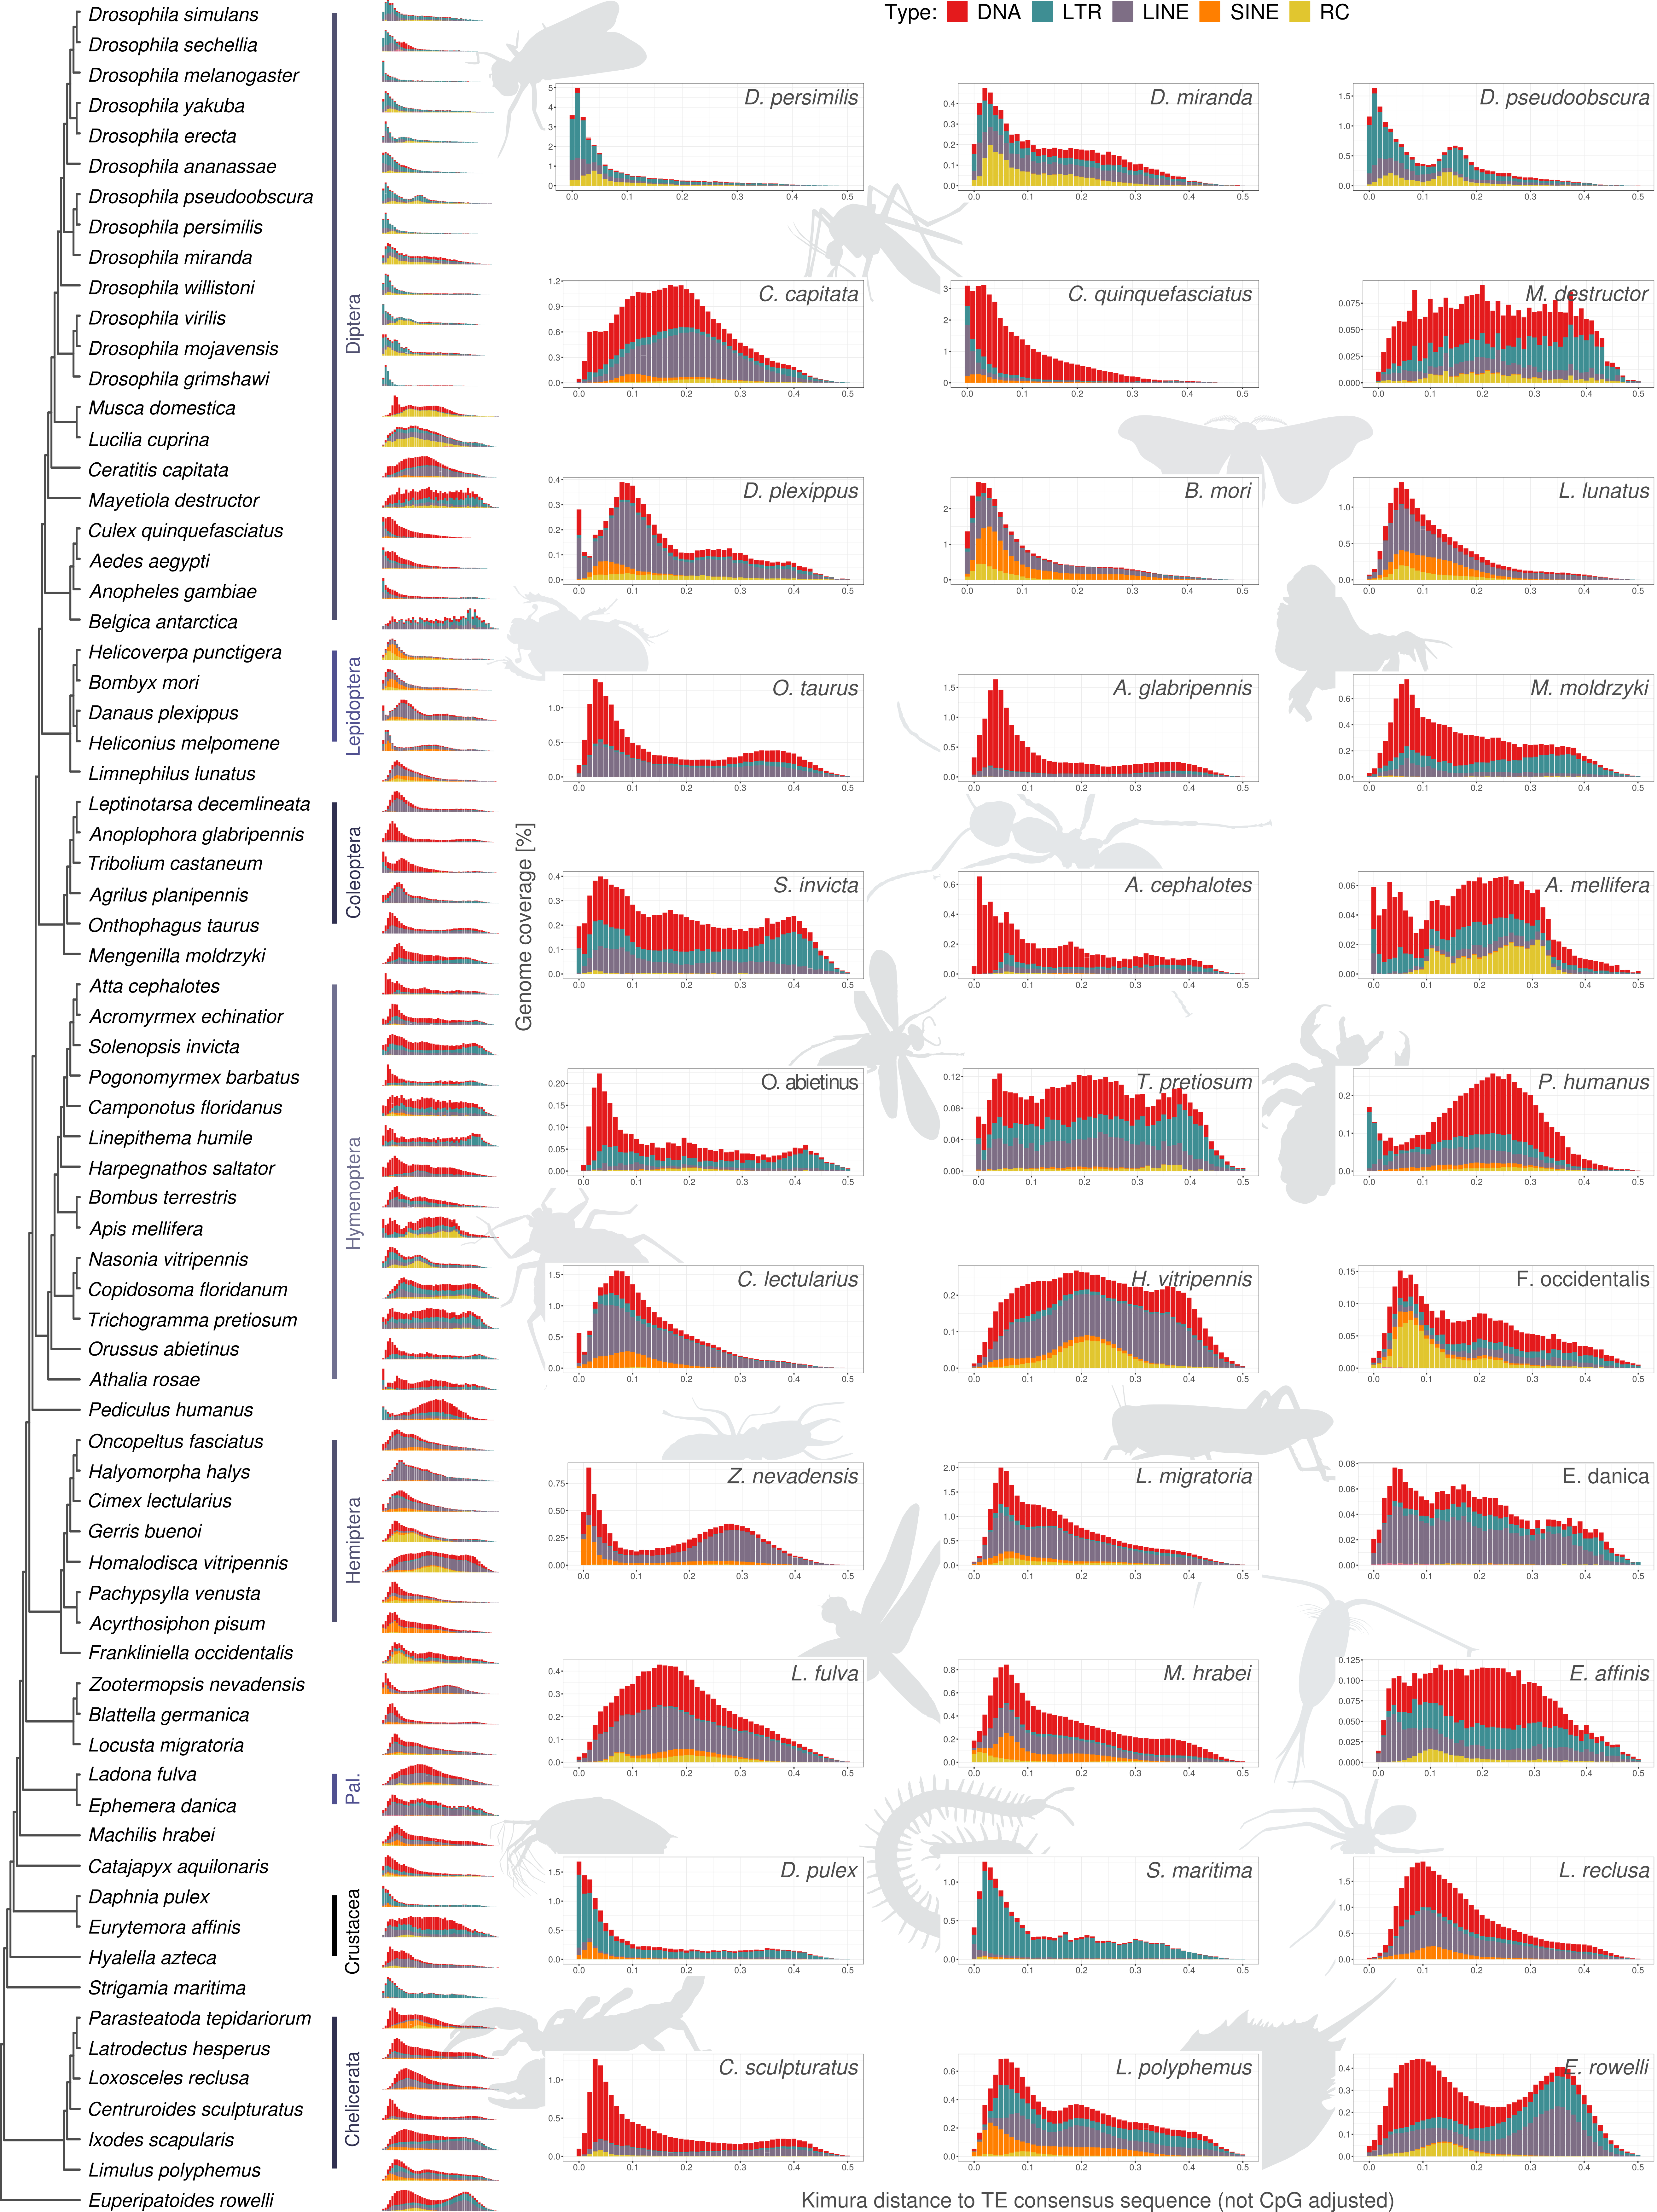
\includegraphics[width=\textwidth]{tree-with-landscapes-and-larger-plots}
\caption[Arthropod repeat landscapes]{{Cladogram with repeat landscape plots. The larger plots are selected
representatives. The further to the left a peak in the distribution is,
the younger the corresponding TE fraction generally is (low TE
intra-family sequence divergence). In most orders, the TE divergence
distribution is similar, such as in Diptera or Hymenoptera. The large
fraction of unclassified elements was omitted for these plots. Pal.,
Palaeoptera%
\label{fig:landscapes}
}}
\end{center}
\end{figure}


In the calyptrate flies, Helitron elements are highly abundant,
representing 28 \% of the genome in the house fly \emph{M. domestica}
and 7 \% in the blow fly \emph{Lucilia cuprina}. These rolling circle
elements are not as abundant in acalyptrate flies, except for the
drosophilids \emph{D. mojavensis}, \emph{D. virilis}, \emph{D. miranda},
and \emph{D. pseudoobscura} (again with a bi-modal distribution). In the
barley midge, \emph{Mayetiola destructor}, DNA transposons occur across
almost all Kimura distances between 0.02 and 0.45. The same holds true
for LTR retrotransposons, although these show an increased expansion in
the older age categories at Kimura distances between 0.37 and 0.44.
LINEs and SINEs as well as Helitron elements show little occurrence in
Diptera. In \emph{B. antarctica}, LINE elements are the most prominent
and exhibit a distribution across all Kimura distances up to 0.4. This
may be a result of the overall low TE concentration in the small
\emph{B. antarctica} genome (less than 1 \%) that introduces stochastic
noise.

In Lepidoptera, we found a relatively recent SINE expansion event around
Kimura distance 0.03 to 0.05. In fact, Lepidoptera and Trichoptera are
the only holometabolous insect orders with a substantial SINE portion of
up to 9 \% in the silk worm \emph{B. mori} (mean: 3.8 \%). We observed
that in the postman butterfly, \emph{Heliconius melpomene}, the SINE
fraction also appears with a divergence between Kimura distances 0.1 to
around 0.31. Additionally, we found high LINE content in the monarch
butterfly \emph{Danaus plexippus} with a divergence ranging from Kimura
distances 0 to 0.47 and a substantial fraction around Kimura distance
0.09.

In all Coleoptera species, we found substantial LINE and DNA content
with a divergence around Kimura distance 0.1. In the beetle species
\emph{Onthophagus taurus}, \emph{Agrilus planipennis}, and \emph{L.
decemlineata}, this fraction consists mostly of LINE copies, while in
\emph{T. castaneum} and \emph{A. glabripennis} DNA elements make up the
major fraction. In all Coleoptera species, the amount of SINEs and
Helitrons is small (cf.~Fig. \ref{fig:te-coverage}). Interestingly, \emph{Mengenilla
moldrzyki}, a representative of Strepsiptera, which was previously
determined to be the sister group of Coleoptera \citep{Niehuis2012},
shows more similarity in TE divergence distribution to Hymenoptera than
to Coleoptera, with a large fraction of DNA elements covering Kimura
distances 0.05 to around 0.3 and relatively small contributions from
LINEs.

In apocritan Hymenoptera (\emph{i.e.}, those with a wasp waist), the DNA
element divergence distribution exhibits a peak around Kimura distance
0.01 to 0.05. In fact, the TE divergence distribution looks very similar
among the ants and differs mostly in absolute coverage, except in
\emph{Camponotus floridanus}, which shows no such distinct peak.
Instead, in \emph{C. floridanus}, we found DNA elements and LTR elements
with a relatively homogeneous coverage distribution between Kimura
distances 0.03 and 0.4. \emph{C. floridanus} is also the only
hymenopteran species with a noticeable SINE proportion; this fraction's
peak divergence is around Kimura distance 0.05. The relatively TE-poor
genome of the honey bee, \emph{Apis mellifera} contains a large fraction
of Helitron elements with a Kimura distance between 0.1 and 0.35, as
does \emph{Nasonia vitripennis} with peak coverage around Kimura
distance 0.15. These species-specific Helitron appearances are likely
the result of an infection from a parasite or virus, as has been
demonstrated in Lepidoptera \citep{Coates2015}. In the (non-apocritan)
parasitic wood wasp, \emph{O. abietinus}, the divergence distribution is
similar to that in ants, with a dominant DNA transposon coverage around
Kimura distance 0.05. The turnip sawfly, \emph{A. rosae} has a large,
zero-divergence fraction of DNA elements, LINEs and LTR retrotransposons
followed by a bi-modal divergence distribution of DNA elements.

When examining Hemiptera, Thysanoptera, and Psocodea, the DNA element
fraction with high divergence (peak Kimura distance 0.25) sets the
psocodean \emph{P. humanus} apart from Hemiptera and Thysanoptera.
Additionally, \emph{P. humanus} exhibits a large peak of LTR element
coverage with a low divergence (Kimura distance 0). In Hemiptera and
Thysanoptera, we found DNA elements with a high coverage around Kimura
distance 0.05 instead of around 0.3, like in \emph{P. humanus}, or only
in miniscule amounts, such as in \emph{Halyomorpha halys}.
Interestingly, the three bug species \emph{H. halys}, \emph{Oncopeltus
fasciatus}, and \emph{Cimex lectularius} show a strikingly similar TE
divergence distribution which differs from that in other species of
Hemiptera. In these species, the TE landscape is characterized by a
wide-ranging distribution of LINE divergence with peak coverage around
Kimura distance 0.07. Further, they exhibit a shallow, but consistent
proportion of SINE coverage with a divergence distribution between
Kimura distance 0 and around 0.3. The other species of Hemiptera and
Thysanoptera show no clear pattern of similarity. In the flower thrips
\emph{Frankliniella occidentalis} (Thysanoptera) as well as in the water
strider \emph{Gerris buenoi} and the cicadellid \emph{Homalodisca
vitripennis}, (Hemiptera), the Helitron elements show a distinct
coverage between Kimura distances 0 and 0.3, with peak coverage at
around 0.05 to 0.1 (\emph{F. occidentalis}, \emph{G. buenoi}) and 0.2
(\emph{H. vitripennis}). In both \emph{F. occidentalis} and \emph{G.
buenoi}, the divergence distribution is slightly bi-modal. In \emph{H.
vitripennis}, LINEs and DNA elements exhibit a divergence distribution
with high coverage at Kimura distances 0.02 to around 0.45. SINEs and
LTR element coverage is only slightly visible. This is in stark contrast
to the findings in the pea aphid \emph{Acyrthosiphon pisum}, where SINEs
make up the majority of the TE content and exhibit a broad spectrum of
Kimura distances from 0 to 0.3, with peak coverage at around Kimura
distance 0.05. Additionally, we found DNA elements in a similar
distribution, but showing no clear peak. Instead, LINEs and LTR elements
are distinctly absent from the \emph{A. pisum} genome, possibly as a
result of a lineage-specific extinction event.

The TE landscape in Polyneoptera is dominated by LINEs, which in the
cockroach \emph{Blattella germanica} have a peak coverage at around
Kimura distance 0.04. In the termite \emph{Zootermopsis nevadensis}, the
peak LINE coverage is between Kimura distances 0.2 and 0.4. In the
locust \emph{L. migratoria}, LINE coverage shows a broad divergence
distribution. Low-divergence LINEs show peak coverage at around Kimura
distance 0.05. All three Polyneoptera species have a small, but
consistent fraction of low-divergence SINE coverage with peak coverage
between Kimura distances 0 to 0.05 as well as a broad, but shallow
distribution of DNA element divergence.



LINEs also dominate the TE landscape in Paleoptera. The mayfly \emph{E.
danica} additionally exhibits a population of LTR elements with medium
divergence in the genome. In the dragonfly \emph{L. fulva}, we found DNA
elements of similar coverage and divergence as the LTR elements. Both TE
types have almost no low-divergence elements in \emph{L. fulva}. In the
early divergent apterygote hexapod orders Diplura (represented by the
species \emph{Catajapyx aquilonaris}) and Archaeognatha (\emph{Machilis
hrabei}), DNA elements are abundant with a broad divergence spectrum and
low-divergence peak coverage. Additionally, we found other TE types with
high coverage in low divergence regions in the genome of \emph{C.
aquilonaris} as well as SINE peak coverage at slightly higher divergence
in \emph{M. hrabei}.

The non-insect outgroup species also exhibit a highly heterogeneous TE
copy divergence spectrum. In all species, we found high coverage of
varying TE types with low divergence. All chelicerate genomes contain
mostly DNA transposons, with LINEs and SINEs contributing a fraction in
the spider \emph{Parasteatoda tepidariorum} and the tick \emph{I.
scapularis}. The only available myriapod genome, that of the centipede
\emph{Strigamia maritima}, is dominated by LTR elements with high
coverage in a low-divergence spectrum, but also LTR elements that
exhibit a higher Kimura distance. We found the same in the crustacean
\emph{Daphnia pulex}, but the TE divergence distribution in the other
crustacean species was different and consisted of more DNA transposons
in the copepod \emph{E. affinis}, or LINEs in the amphipod
\emph{Hyalella azteca}.

\section{Discussion}

We used species-specific TE libraries to assess the genomic retrotransposable and transposable element content in sequenced and assembled genomes of arthropod species, including most extant insect orders.

\subsection{TE content contributes to genome size in
arthropods}

TEs and other types of DNA repeats are an omnipresent part of metazoan,
plant, as well as fungal genomes and are found in variable proportions
in sequenced genomes of different species. In vertebrates and plants,
studies have shown that TE content is a predictor for genome size
\citep{Chalopin2015,Staton2015}. For insects, this has also been reported in
clade-specific studies such as those on mosquitoes \citep{Neafsey2015}
and \emph{Drosophila} fruit flies \citep{Sessegolo2016}. These observations
lend further support to the hypothesis that genome size is also
correlated with TE content in insects on a pan-ordinal scale.

Our analysis shows that both genome size and TE content are highly
variable among the investigated insect genomes, even in comparative
contexts with low variation in genome size. While non-holometabolous
hexapods have a significantly smaller genome than holometabolous
insects, the TE content is not significantly different. Still, we found
that TE content contributes significantly to genome size in hexapods as
a whole. These results are in line with prior studies on insects with a
more limited taxon sampling reporting a clade-specific correlation
between TE content and genome size \citep{Vieira1999,Vieira2002,Kidwell2000,Honeybee2006,Bosco2007,Sessegolo2016}, and expand that
finding to larger taxon sampling covering most major insect orders.
These findings further support the hypothesis that TEs are a major
factor in the dynamics of genome size evolution in Eukaryotes. While
differential TE activity apparently contributes to genome size variation
\citep{Petrov2001,Kidwell2002,Agren2011}, whole genome duplications, such as suggested by
integer-sized genome size variations in some representatives of
Hymenoptera \citep{Li2018}, segmental duplications, deletions, and
other repeat proliferation \citep{Parfrey2008} could contribute as well.
This variety of influencing factors potentially explains the range of
dispersion in the correlation.

The high range of dispersion in the correlation of TE content and genome
size is most likely also amplified by heterogeneous underestimates of
the genomic TE coverage. Most of the genomes were sequenced and
assembled using different methods, and with insufficient sequencing
depth and/or older assembly methods; the data are therefore almost
certainly incomplete with respect to repeat-rich regions. Assembly
errors and artifacts also add a possible error margin, as assemblers
cannot reconstruct repeat regions that are longer than the insert size
accurately from short reads \citep{Schatz2010,Sambaturu2014,Chaisson2015,Peona2018} and most available
genomes were sequenced using short read technology only. Additionally,
RepeatMasker is known to underestimate the genomic repeat content
\citep{deKoning2011}. By combining RepeatModeler to infer the
species-specific repeat libraries and RepeatMasker to annotate the
species-specific repeat libraries in the genome assemblies, our methods
are purposefully conservative and may have missed some TE types, or
ancient and highly divergent copies.

This underestimation of the TE content notwithstanding, we found many TE
families that were previously thought to be restricted to, for example,
mammals, such as the SINE family Alu \citep{Kriegs2007} and the LINE
family L1 \citep{Liu2003}, or to fungi, such as Tad1
\citep{Cambareri1994}. Essentially, most known superfamilies were found in
the investigated insect genomes (\emph{cf}. Fig. \ref{fig:presence-absence}) and additionally, we
identified highly abundant unclassifiable TEs in all insect species.
These observations suggest that the insect mobilome (the entirety of
mobile DNA elements) is more diverse than the well characterized
vertebrate mobilome \citep{Chalopin2015} and requires more exhaustive
characterization. We were able to reach these conclusions by relying on
two essential non-standard analyses. First, our annotation strategy of
\emph{de novo} repeat library construction and classification according
to the RepBase database was more specific to each genome than the
default RepeatMasker analysis using only the RepBase reference library.
The latter approach is usually done when releasing a new genome assembly
to the public. The second difference between our approach and the
conventional application of the RepBase library was that we used the
entire Metazoa-specific section of RepBase instead of restricting our
search to Insecta. This broader scope allowed us to annotate TEs that
were previously unknown from insects, and that would otherwise have been
overlooked. Additionally, by removing results that matched non-TE
sequences in the NCBI database, our annotation becomes more robust
against false positives. The enormous previously overlooked diversity of
TEs in insects does not seem to be surprising given the geological age
and species richness of this clade. Insects originated more than 450
million years ago \citep{Misof2014} and represent over 80 \% of the
described metazoan species \citep{Grimaldi2005}. Further investigations
will also show whether there is a connection between TE diversity or
abundance and clade-specific genetic and genomic traits, such as the sex
determination system (\emph{e.g.}, butterflies have Z and W chromosomes
instead of X and Y \citep{Traut1997}) or the composition of telomeres,
which have been shown in \emph{D. melanogaster} to exhibit a high
density of TEs \citep{Levis1993}, whereas telomeres in other insects
consist mostly of simple repeats. It remains to be analyzed in detail,
however, whether insect TE diversity evolved independently within
insects or is the result of multiple TE introgression into insect
genomes.

Our results show that virtually all known TE classes are present in all investigated insect genomes.
However, a large part of the TEs we identified remains unclassifiable despite the diversity of metazoan TEs in the reference library RepBase.
This abundance of unclassifiable TEs suggests that the insect TE repertoire requires more exhaustive characterization and that our understanding of the insect mobilome is far from complete.

It has been hypothesized that population-level processes might
contribute to TE content differences and genome size variation in
vertebrates \citep{Lynch2003}. In insects, it has been shown that TE
activity also varies on the population level, for example in the genomes
of \emph{Drosophila} spp. \citep{Perrat2013,Li2013,Blumenstiel2014} or in the genome of the
British peppered moth \emph{Biston betularia}, in which a tandemly
repeated TE confers an adaptive advantage in response to short-term
environmental changes \citep{Hof2016}. The TE activity within
populations is expected to leave footprints in the nucleotide sequence
diversity of TEs in the genome as recent bursts of TEs should be
detectable by a large number of TE sequences with low sequence
divergence.

To explain TE proliferation dynamics, two different models of TE
activity have been proposed: the equilibrium model and the burst model.
In the equilibrium model, TE proliferation and elimination rates are
more or less constant and cancel each other out at a level that is
different for each genome \citep{Charlesworth1983}. In this model,
differential TE elimination rate contributes to genome size variation
when TE activity is constant. This model predicts that in species with a
slow rate of DNA loss, genome size tends to increase \citep{Petrov2011,Sun2011}.
In the burst model, TEs do not proliferate at a constant rate, but
rather in high copy rate bursts following a period of inactivity
\citep{Blumenstiel2014}. These bursts can be TE family specific. Our analysis
of TE landscape diversity (see below), supports the burst hypothesis. In
almost every species we analyzed, there is a high proportion of abundant
TE sequences with low sequence divergence and the most abundant TEs are
different even among closely related species. It was hypothesized that
TE bursts enabled by periods of reduced efficiency in counteracting host
defense mechanisms such as TE silencing \citep{LeRouzic2006,Rebollo2010} have resulted
in differential TE contribution to genome size.

\subsection{TE landscape diversity in
arthropods}

In vertebrates, it is possible to trace lineage-specific contributions
of different TE types \citep{Chalopin2015}. In insects, however, the TE
composition shows a statistically significant correlation to genome
size, but a high range of dispersion. Instead, we can show that major
differences both in TE abundance and diversity exist between species of
the same lineage (Fig. \ref{fig:presence-absence}). Using the Kimura nucleotide sequence
distance, we observe distinct variation, but also similarities, in TE
composition and activity between insect orders and among species of the
same order. The number of recently active elements can be highly
variable, such as LTR retrotransposons in fruit flies or DNA transposons
in ants (Fig. \ref{fig:landscapes}). On the other hand, the shape of the TE coverage
distributions can be fairly similar among species of the same order;
this is particularly visible in Hymenoptera and Diptera. These findings
suggest lineage-specific similarities in TE elimination mechanisms;
possibly shared efficacies in the piRNA pathway that silences TEs during
transcription in metazoans (\emph{e.g.}, in \emph{Drosophila}
\citep{LeThomas2013,Yamashiro2017}, \emph{B. mori} \citep{Matsumoto2016},
\emph{Caenorhabditis elegans} \citep{Zhang2018}, and mouse
\citep{Toth2016}. Another possible explanation would be recent
horizontal transfers from, for example, parasite to host species (see
below).

\subsection{Can we infer an ancestral arthropod mobilome in the face of
massive horizontal TE
transfer?}

In a purely vertical mode of TE transmission, the genome of the last
common ancestor (LCA) of insects --- or arthropods --- can be assumed to
possess a superset of the TE superfamilies present in extant insect
species. As many TE families appear to have been lost due to
lineage-specific TE extinction events, the ancestral TE repertoire may
have been even more extensive compared with the TE repertoire of extant
species and might have included almost all known metazoan TE
superfamilies such as the CMC complex, Ginger, Helitron, Mavericks,
Jockey, L1, Penelope, R1, DIRS, Ngaro, and Pao. Many SINEs found in
extant insects were most likely part of the ancestral mobilome as well,
for example Alu, which was previously thought to be restricted to
primates \citep{Deininger2011}, and MIR.

The mobilome in extant species, however, appears to be the product of
both vertical and horizontal transmission. In contrast to a vertical
mode of transmission, horizontal gene transfers, common phenomenona
among prokaryotes (and making a prokaryote species phylogeny nigh
meaningless) and widely occurring in plants, are rather rare in
vertebrates \citep{Syvanen2012,Wallau2012}, but have been described in Lepidoptera
\citep{Sormacheva2012} and other insects \citep{Nakabachi2015}. Recently, a
study uncovered large-scale horizontal transfer of TEs (horizontal
transposon transfer, HTT) among insects \citep{Peccoud2017} and makes
this mechanism even more likely to be the source of inter-lineage
similarities in insect genomic TE composition. In the presence of
massive HTT, the ancestral mobilome might be impossible to infer because
the effects of HTT overshadow the result of vertical TE transfer. It
remains to be analyzed in detail whether the high diversity of the
insect mobilomes can be better explained by massive HTT events.

\section{Conclusions}

The present study provides an overview of the diversity and evolution of TEs in the genomes of major lineages of extant insects.
The results show that there is large intra- and inter-lineage variation in both TE content and composition.
This, and the highly variable age distribution of individual TE superfamilies, indicate a lineage-specific burst-like mode of TE proliferation in insect genomes.
In addition to the complex composition patterns that can differ even among species of the same genus, there is a large fraction of TEs that remain unclassified, but often make up the major part of the genomic TE content, indicating that the insect mobilome is far from completely characterized.
This study provides a solid baseline for future comparative genomics research.
The functional implications of lineage-specific TE activity for the evolution of genome architecture will be the focus of future investigations.


%!TEX root = ../dissertation.tex
%--------------------------------------------------
% \begin{savequote}[75mm]
% \qauthor{Quoteauthor Lastname}
% \end{savequote}
%-------------------------------------------------- 

\chapter{Dynamics of genome size evolution in insects}
\label{cha:dynamics}
This chapter is intended for publication in \emph{PNAS}.

Authors: Petersen, M., Nottebrock G., Misof, B. 

Author contributions: Analyses: MP, GN, figures: MP, GN, manuscript
design and writing: MP, GN, BM

\section{Introduction}

Genome size variation is an important aspect of eukaryote genome
evolution \citep{Gregory2005,Petrov2001} and seems positively correlated with cell
size \citep{Dufresne2011}, and body size in invertebrates
\citep{Gregory2008}. It has also been reported that genome size is
positively correlated with cell division time \citep{Bennett1977} and
developmental rate \citep{White2000}. Genome size variation, however,
does not appear to be correlated with organismic complexity (the
so-called c-value enigma \citep{Gregory2008}). It is currently unclear
how genome size variation and the evolution of phenotypic traits are
correlated.

Genome size can expand because of, for example, whole or partial genome
duplications, or the accumulation of transposable elements
\citep{Bennetzen2005,Piegu2006,Vitte2007,Kelly2015,Nystedt2013,Blass2012,Neafsey2003,Sun2012,Sato2010,Marburger2018,Kapusta2017a}. Genome size expansion and contraction have been
found to be correlated with the frequency of transposable elements (TEs)
in the genome \citep{Sotero-Caio2017,Kapusta2017a,Petrov1996,Petrov2000}. TEs play a pivotal role in functional
adaptation and genome evolution in general that is not yet fully
understood (reviewed in \citet{Maumus2015,Arkhipova2018}).

For mammals and birds, an ``accordion'' model of genome size dynamics
has been proposed \citet{Kapusta2017a} that predicts a more or less
stable genome size over time. This genome size stability in the presence
of TE activity has also been termed the equilibrium model by
\citet{Charlesworth1983}. According to this model, genome expansion due to TE
activity is counteracted by DNA removal, resulting in little
fluctuations in genome size. In arthropods, however, where most
taxonomic orders are much older than the mammal and bird lineages
\citep{Misof2014}, genome size varies strongly \citep{Alfsnes2017,Petersen2019};
this variation has been connected to, but is not entirely explained by
TE content. Additionally, the TE landscape suggests a more burst-like
activity profile in arthropods \citep{Petersen2019}.

In the present study, we exploit the growing number of sequenced
arthropod genomes and assess genomic DNA gain and loss caused by TE
activity. Our results are inconsistent with an ``accordion'' or
equilibrium model of genome size dynamics, therefore we propose that
genome size in insects is governed by different, more burst-like
dynamics than in mammals and birds.

\section{Materials and Methods}

\subsection*{Ancestral genome size
estimation}

To determine the age of TE copies in the insect genomes, we first
estimated clade-specific ancestral genome sizes with the approach
described in the following. We sourced the Animal Genome Size Database
\citep{Gregory2018} (\url{http://genomesize.com}, accessed 2018-05-01) to
obtain genome size estimates for 1,514 arthropod species. Additionally,
we exploited the BOLD database \citep{Ratnasingham2007}
(\url{http://www.boldsystems.org}, accessed 2018-03-19) to obtain
1,571,820 COI barcode nucleotide sequences for 105,397 arthropod
species. Of these, we identified 605 species that were represented in
both databases. We included our own genome size estimates for eight
additional species (Supplemental Table \ref{tab:genome-size-estimates}), bringing the total number of
species to 613.

For the dipluran \emph{Catajapyx aquilonaris}, which was not represented
in the BOLD database, we added COI data by retrieving a COI sequence
from the closely related species \emph{Gollumjapyx smeagol} (GenBank ID
DQ993154.1) and using it as query in a BLAST search in the genome
assembly provided by the i5k initiative (source see Supplemental Table
\ref{tab:genome-assemblies}). We received two hits and used the longer one
(scaffold131247\_cov1551 positions 852-1522) as query in a BLAST search
in GenBank. The reciprocal search hit the mitochondrial genome of
\emph{Japyx solifugus} (Accession AY771989.1), another closely related
species, which confirmed that our hit was indeed the COI sequence of
\emph{C. aquilonaris}.

To obtain a phylogenetic tree with branch length estimates, we first
compiled a constraint tree topology from the literature. The arthropod
order topology was taken from \citet{Misof2014}. We computed multiple
sequence alignments from the COI sequences for each order separately
using MAFFT v7.309. We removed redundant sequences and sequences that
could not be translated without having stop codons, and inferred ML
phylogenies for each order using RAxML v8.2.11. We manually corrected
these order-specific topologies using published phylogenies (reference
list in Supplemental Table \ref{tab:phylogeny-sources}). For those species without placement from
the literature, we used the COI topology under majority-rule consensus
in case there were more than one COI sequence. We combined the
order-specific trees into a large tree and used that topology as
constraint to estimate branch lengths using RAxML.

The resulting tree was rendered ultrametric by a short Python script
using the ETE toolkit \citep{Huerta-Cepas2016} (see Supplemental Material). To
time-calibrate the phylogeny, we selected calibration points from
\citep{Misof2014} (Table \ref{tab:calibration-points}) and used the \texttt{chronos} function
from the ape package in R to adjust the branch lengths. We used the
upper and lower bounds of the 95 \% confidence interval as minimum and
maximum node ages. We set \(\lambda\) to 2 and used the discrete
model. We used the \texttt{fastAnc} ML implementation in the phytools
package \citep{Revell2012} in R to infer ancestral genome sizes using
the Ornstein-Uhlenbeck model for each node along the tree including 95
\% confidence intervals.

\subsection*{Genomic datasets and genome size
estimates}

The genome assembly accession numbers and data sources of 96 arthropod
species are listed in Supplemental Table \ref{tab:genome-assemblies}. The genome assemblies were
downloaded from NCBI (69 species) or from the i5k FTP server (27
species). Genome size estimates were obtained from the Animal Genome
Size Database (\citet{Gregory2018}, \url{http://genomesize.com}),
measured in our own lab using flow cytometry (FCM), or estimated using a
\emph{k}-mer peak method adopted from \citet{Hozza2015}. Our own
estimate results are listed in Supplemental Table
\ref{tab:genome-size-estimates}.

\subsection*{Transposable element
annotation}

We used a pipeline for repeat annotation from \citet{Petersen2019} that
employs RepeatModeler 1.0.10 \citep{Smit2015a} to infer a
species-specific repeat consensus library from each genome assembly, and
RepeatMasker 4.0.5 \citep{Smit2015} to annotate TE copies in the
genome assemblies. The annotation by RepeatModeler includes a
substantial fraction of ``Unknown'' elements, so the pipeline employs an
intermediate filtering step to exclude false positives. We used NCBI
BLAST to search the consensus libraries in the NCBI non-redundant
nucleotide database, and removed all ``Unknown'' consensus sequences
that did not result in a hit on a known TE protein. We also removed
annotations shorter than 50 nucleotides.

To infer accurate TE content estimates and TE ages from the RepeatMasker
annotation results, we developed a Perl program that uses the Kimura
distance of each TE copy from the TE consensus sequence and the
order-specific nucleotide substitution rate to infer the age of each TE
copy in million years (My). The Perl code is available at
\href{https://github.com/mptrsen/dynamics-of-genome-size}{this study's
Github repository}. We used a time-calibrated phylogeny of insects
\citep{Misof2014} and multiple sequence alignments of 1,478
protein-coding genes from 144 arthropod species \citep{Misof2014} to
infer order-specific nucleotide substitution rates by using the weighted
arithmetic mean of substitution rates (see equation
(\ref{eqn:weighted-arithmetic-mean}) in Supplemental
material, page \pageref{eqn:weighted-arithmetic-mean}). The program also takes into account that TE annotations
sometimes overlap each other by distributing the count of affected
nucleotide positions as fractions evenly among overlapping TE copies.
While this approach results in decimal instead of integer TE lengths, it
provides a better estimate of the amount of nucleotides covered by TEs
as it handles each element equally. The corrected lengths were only used
in the TE content counts, not in the age estimations.

\subsection*{DNA gain and loss}

Using the time-calibrated phylogeny and the TE age inferences, we
classified TE copies into clade-specific and ancient (a TE copy was
classified as ancient if it was older than the most recent split of the
clade it was found in to the sister clade, otherwise as
lineage-specific). For Chelicerata and Myriapoda, we took clade
divergence times from \citet{Misof2014} (all divergence times are
listed in Table \ref{tab:species-divergence-times}). We calculated the amount of DNA gained by TE
proliferation as the amount of clade-specific TEs.

With the ancestral genome sizes and the inferred amounts of DNA gained
by TE activity, we computed the amount of ancestral DNA in the extant
genomes by subtracting the amounts of lineage-specific TE material from
the extant genome assembly sizes. This allowed us to infer the amount of
ancestral DNA that was lost since the common ancestor of the clade for
each arthropod lineage by subtracting the amount of ancestral DNA from
the estimated ancestral genome size.

We computed the DNA loss coefficient \(k\) (1) according to
\citet{Lindblad-Toh2005} as \(E = A e^{-kt}\), where \(E\) is
the amount of extant ancestral sequence in the genome assembly,
\(A\) the total ancestral assembly size, and
\(t\) the time since the split from the last ancestor.

\begin{equation}
k = \frac{\ln{\frac{A}{E}}}{t}
\end{equation}

\section{Results}

\subsection*{Ancestral genome size
reconstruction}

We reconstructed ancestral genome sizes (see Methods) of 613 arthropod
species with published phylogenetic relationships (refs. listed in
Supplemental Table \ref{tab:phylogeny-sources}), amended with branch lengths inferred from COI
barcode sequences, and genome size estimates for extant species obtained
from the genome size database \citep{Gregory2018}. We inferred an
ancestral genome size for the root node of hexapods (node \textbf{1})
between 782 and 1943 Mbp (95 \% confidence interval) (Figure
\ref{fig:tree-with-ancestral-sizes}). This
inferred genome size is well above the maximum of many holometabolous
clades such as Diptera (node \textbf{2}, 272 to 545 Mbp), Lepidoptera
(node \textbf{3}, 318 to 738 Mbp), or Hymenoptera (node \textbf{4}, 303
to 633 Mbp) (Table \ref{tab:ancestral-sizes}), but within the range of hemimetabolan orders,
except for Orthoptera (node \textbf{5}), of which the ancestral size was
inferred to be between 3,677 and 9,473 Mbp. This is not surprising given
the genome sizes of extant representatives of Orthoptera between 2 Gbp
in \emph{Acheta domesticus} and 16.5 Gbp in \emph{Podisma pedestris}.

\begin{longtable}{lrrrr}
\caption[Inferred ancestral genome size for major arthropod orders]{Inferred ancestral genome sizes for major arthropod orders using the
Ornstein-Uhlenbeck model. Ancestral size refers to the median, upper and
lower bounds refer to the bounds of the 95\% confidence interval (CI).
All values in Mbp.
\label{tab:ancestral-sizes}}%
\footnotesize
\endfirsthead


\multicolumn{5}{c}{%
{\tablename\ \thetable{} --continued}} \\
\toprule
Clade & Node & Anc. size & Lower bound & Upper bound \\
\midrule
\endhead

\bottomrule
\endfoot

Clade & Node & Anc. size [Mbp] & Lower bound & Upper bound \\
\midrule
Diptera & 2 & 340.65 & 251.41 & 461.57 \\
Diptera:Telmatogeton+Chironomus & 17 & 242.47 & 165.97 & 354.25 \\
Diptera:Drosophila & 18 & 268.96 & 201.7 & 358.65 \\
Diptera:Aedes & 21 & 850.17 & 590.84 & 1223.32 \\
Mecoptera &  & 411.94 & 281.49 & 602.85 \\
Lepidoptera & 3 & 478.6 & 333.79 & 686.23 \\
Lepidoptera:Papilionidae & 6 & 368.1 & 236.45 & 573.04 \\
Lepidoptera:Drepanidae & 7 & 379.0 & 246.92 & 581.73 \\
Lepidoptera:Geometridae & 8 & 591.34 & 400.93 & 872.18 \\
Lepidoptera:Notodontidae & 9 & 427.97 & 279.38 & 655.57 \\
Lepidoptera:Erebidae & 10 & 742.04 & 519.66 & 1059.59 \\
Lepidoptera:Euchaetes+Lymantria & 20 & 828.79 & 599.19 & 1146.37 \\
Trichoptera &  & 527.27 & 339.93 & 817.85 \\
Neuropterida &  & 512.92 & 273.37 & 962.38 \\
Coleoptera &  & 565.59 & 385.45 & 829.92 \\
Coleoptera:Callosobruchus & 12 & 1037.25 & 694.8 & 1548.49 \\
Coleoptera:Carabidae & 13 & 321.01 & 207.3 & 497.11 \\
Coleoptera:Tribolium & 16 & 303.52 & 198.64 & 463.78 \\
Coleoptera:Tenebrionidae & 11 & 467.36 & 303.29 & 720.18 \\
Coleoptera:Dermestidae & 19 & 903.72 & 559.72 & 1459.12 \\
Strepsiptera & 14 & 192.46 & 105.68 & 350.49 \\
Hymenoptera & 4 & 418.05 & 280.94 & 622.08 \\
Hymenoptera:base & 15 & 242.59 & 139.94 & 420.54 \\
Condylognatha &  & 741.39 & 471.34 & 1166.16 \\
Psocodea &  & 705.64 & 472.19 & 1054.53 \\
Hemiptera &  & 778.22 & 496.61 & 1219.52 \\
Sternorrhyncha &  & 676.04 & 416.06 & 1098.48 \\
Heteroptera &  & 1056.97 & 642.94 & 1737.61 \\
Auchenorryncha &  & 1404.28 & 785.17 & 2511.56 \\
Thysanoptera &  & 514.07 & 268.12 & 985.63 \\
Polyneoptera &  & 1623.44 & 996.76 & 2644.11 \\
Blattodea+Isoptera &  & 1685.6 & 969.63 & 2930.26 \\
Isoptera &  & 1391.74 & 843.35 & 2296.74 \\
Phasmatodea &  & 1770.0 & 960.52 & 3261.7 \\
Orthoptera & 5 & 2659.61 & 1580.63 & 4475.16 \\
Odonata &  & 917.39 & 562.65 & 1495.78 \\
Ephemeroptera &  & 887.61 & 538.95 & 1461.83 \\
Palaeoptera &  & 887.61 & 538.95 & 1461.83 \\
Diplura &  & 990.59 & 504.5 & 1945.06 \\
Archaeognatha &  & 1630.8 & 828.79 & 3208.93 \\
Ellipura &  & 990.59 & 504.5 & 1945.06 \\
Collembola &  & 990.59 & 504.5 & 1945.06 \\
Zygentoma &  & 1002.05 & 629.0 & 1596.35 \\
Hexapoda & 1 & 990.59 & 504.5 & 1945.06 \\
Crustacea &  & 2043.45 & 1122.58 & 3719.73 \\
Copepoda+Branchiopoda &  & 1364.13 & 773.59 & 2405.49 \\
Branchiopoda &  & 973.39 & 524.83 & 1805.31 \\
Copepoda &  & 1256.67 & 714.34 & 2210.73 \\
Malacostraca &  & 3186.87 & 1774.25 & 5724.16 \\
\end{longtable}

\bigskip

In some orders, we inferred a dynamic pattern of genome size evolution.
For example within Lepidoptera, Papilionidae (node \textbf{6}) have the
smallest inferred ancestral genome size among Lepidoptera (median size:
358 Mbp), or the two sister groups Drepanidae and Geometridae (nodes
\textbf{7} and \textbf{8}) differ in their inferred ancestral genome
size more than twofold (\emph{Drepana} species (Drepanidae), median
size: 318 Mbp; \emph{Scopula limboundata} (Geometridae), median size:
870 Mbp), as is also the case for the two sister groups Notodontidae
(node \textbf{9}, \emph{e.g.}, \emph{Nadata gibbosa}; median size: 352
Mbp) and Erebidae (node \textbf{10}, \emph{e.g.}, \emph{Malacosoma
disstria}; median size: 636 Mbp). A similar dynamics in inferred
ancestral genome size variation is visible in Coleoptera: Tenebrionidae
(node \textbf{11}, such as species of the genus \emph{Tribolium}) have
small inferred ancestral genomes (median size: 235 Mbp) in contrast to
species of the Cleridae/Silvanidae/Chrysomelidae/Curculionidae complex
with large inferred ancestral genomes (\emph{e.g.},
\emph{Callosobruchus}, node \textbf{12}; median: 836 Mbp). Within
Carabidae (node \textbf{13}), species of the genus \emph{Carabus} have
inferred ancestral genome sizes of about 245 Mbp, in stark contrast to
the other carabid species such as \emph{Calosoma scrutator} (1,017 Mbp).

\begin{figure}[h!]
\begin{center}
\includegraphics[width=\textwidth]{COI-tree-with-genome-sizes-log}
\caption[Ancestral genome size reconstruction]{{Ancestral genome size
reconstruction reveals highly dynamic insect genomes. Chronogram based
on published phylogenies and branch lengths estimated from COI
nucleotide sequences. The branch coloration represents the inferred
ancestral genome size (red: small, green: medium, blue: large). Red
arrows denote species that are included in the TE age analysis. This
figure is also appended in A2 poster format to the end of this thesis.
{\label{fig:tree-with-ancestral-sizes}}%
}}
\end{center}
\end{figure}

The smallest extant and ancestral inferred genome size was found in
Strepsiptera (node \textbf{14}) (inferred genome size of the most recent
common ancestor (MRCA): 104 to 349 Mbp, with the extant \emph{Xenos
vesparum} having 127 Mbp). The ancestral holometabolan genome was
inferred to be between 390 and 751 Mbp in size. Holometabola, however,
appear to have undergone several events of genome size contraction
according to our reconstructions (smaller than the holometabolan
ancestor). Examples of smaller genome sizes than the holometabolan
ancestor include the MRCA of basal Hymenoptera such as
\emph{Macrocentrus cingulum}, \emph{Aphidius colemani}, and
\emph{Aphidius ervi} (node \textbf{15}) with an inferred ancestral
genome size between 140 and 420 Mbp; similarly, we inferred a genome
size of 199 to 464 Mbp for the MRCA of the \emph{Tribolium} beetle genus
(node \textbf{16}). Likewise, we inferred smaller genomes for the MRCA
of the nematoceran flies \emph{Telmatogeton japonicus} and
\emph{Chironomus plumosus} (Diptera, node \textbf{17}, 166 to 354 Mbp)
and of the \emph{Drosophila} group (node \textbf{18}, 202 to 359 Mbp).
Our inferences also include examples of genome expansion (larger than
the holometabolan ancestor). For example, the MRCA of dermestid beetles
(node \textbf{19}) had an inferred genome size between 560 and 1,459
Mbp); the MRCA genome of \emph{Lymantria dispar} and \emph{Euchaetes
egle} (Lepidoptera, node \textbf{20}) was inferred to be between 520 and
1,060 Mbp, and the MRCA genome of the \emph{Aedes} mosquito genus (node
\textbf{21}) was inferred to be between 591 and 1,224 Mbp. These results
also contradict prior suggestions that Holometabola generally have
smaller genomes than Hemimetabola, \emph{e.g.}, by \citet{Hanrahan2011}.

\subsection*{Transposable elements contribute to genome size
variation}

We investigated the correlation between genome size and TE content. In
order to do so, we annotated TEs in 96 arthropod genomes using a
pipeline that combines RepeatModeler \citep{Smit2015a} and RepeatMasker
\citep{Smit2015} and found that genome size correlates with TE content
(PIC \citep{Felsenstein1985}, Pearson's product moment correlation,
\(p = 0.0003484\)). We also inferred the age in million years for each
TE copy using order-specific nucleotide substitution rates and the
Kimura 2-parameter distance of each TE copy from the TE family consensus
reported by RepeatMasker (see Methods). The median ages (Figure
\ref{fig:age-mediane}, page \pageref{fig:age-mediane}) of all TE classes within species are
significantly correlated with the divergence times of the respective
species, but only LINEs show this correlation also when applying PIC
(Kendall's rank correlation, \(p = 0.04\)).

Using divergence times from the dated phylogeny based on the literature
(see above), we classified the TE content into lineage-specific copies
(younger than the age of the lineage, \emph{i.e.}, the split of the
species with its last common ancestor) and ancient copies (older than
the lineage). In 36 out of 53 insect species that were represented in
the dated tree, we found more than 99 \% lineage-specific TEs (Figure
\ref{fig:age-vs-perc-ancestral} on page
\pageref{fig:age-vs-perc-ancestral},
Supplemental Figure \ref{fig:agesplit}). Notable exceptions included the termite
\emph{Zootermopsis} with 86.3 \% ancestral TEs, the bumblebee
\emph{Bombus terrestris} with 81.1 \% ancestral TEs, and the dragonfly
\emph{Calopteryx splendens} with 82 \% ancestral TEs. The closely
related \emph{Drosophila} species displayed great variation in the
ancestral TE fraction, ranging from 0.85 \% in \emph{D. mojavensis} to
47.4 \% in \emph{D. simulans}. We tested for phylogenetic signal using
Blomberg's \emph{K} and found low signal in the ancestral TE fraction
(\(K = 0.1\), \(p = 0.9\)). The fraction of ancestral TEs
is significantly correlated with the age of the lineage under
phylogenetically independent contrasts (PIC) (Kendall,
\(p = 2e-10\)).

\begin{figure}[h!]
\begin{center}
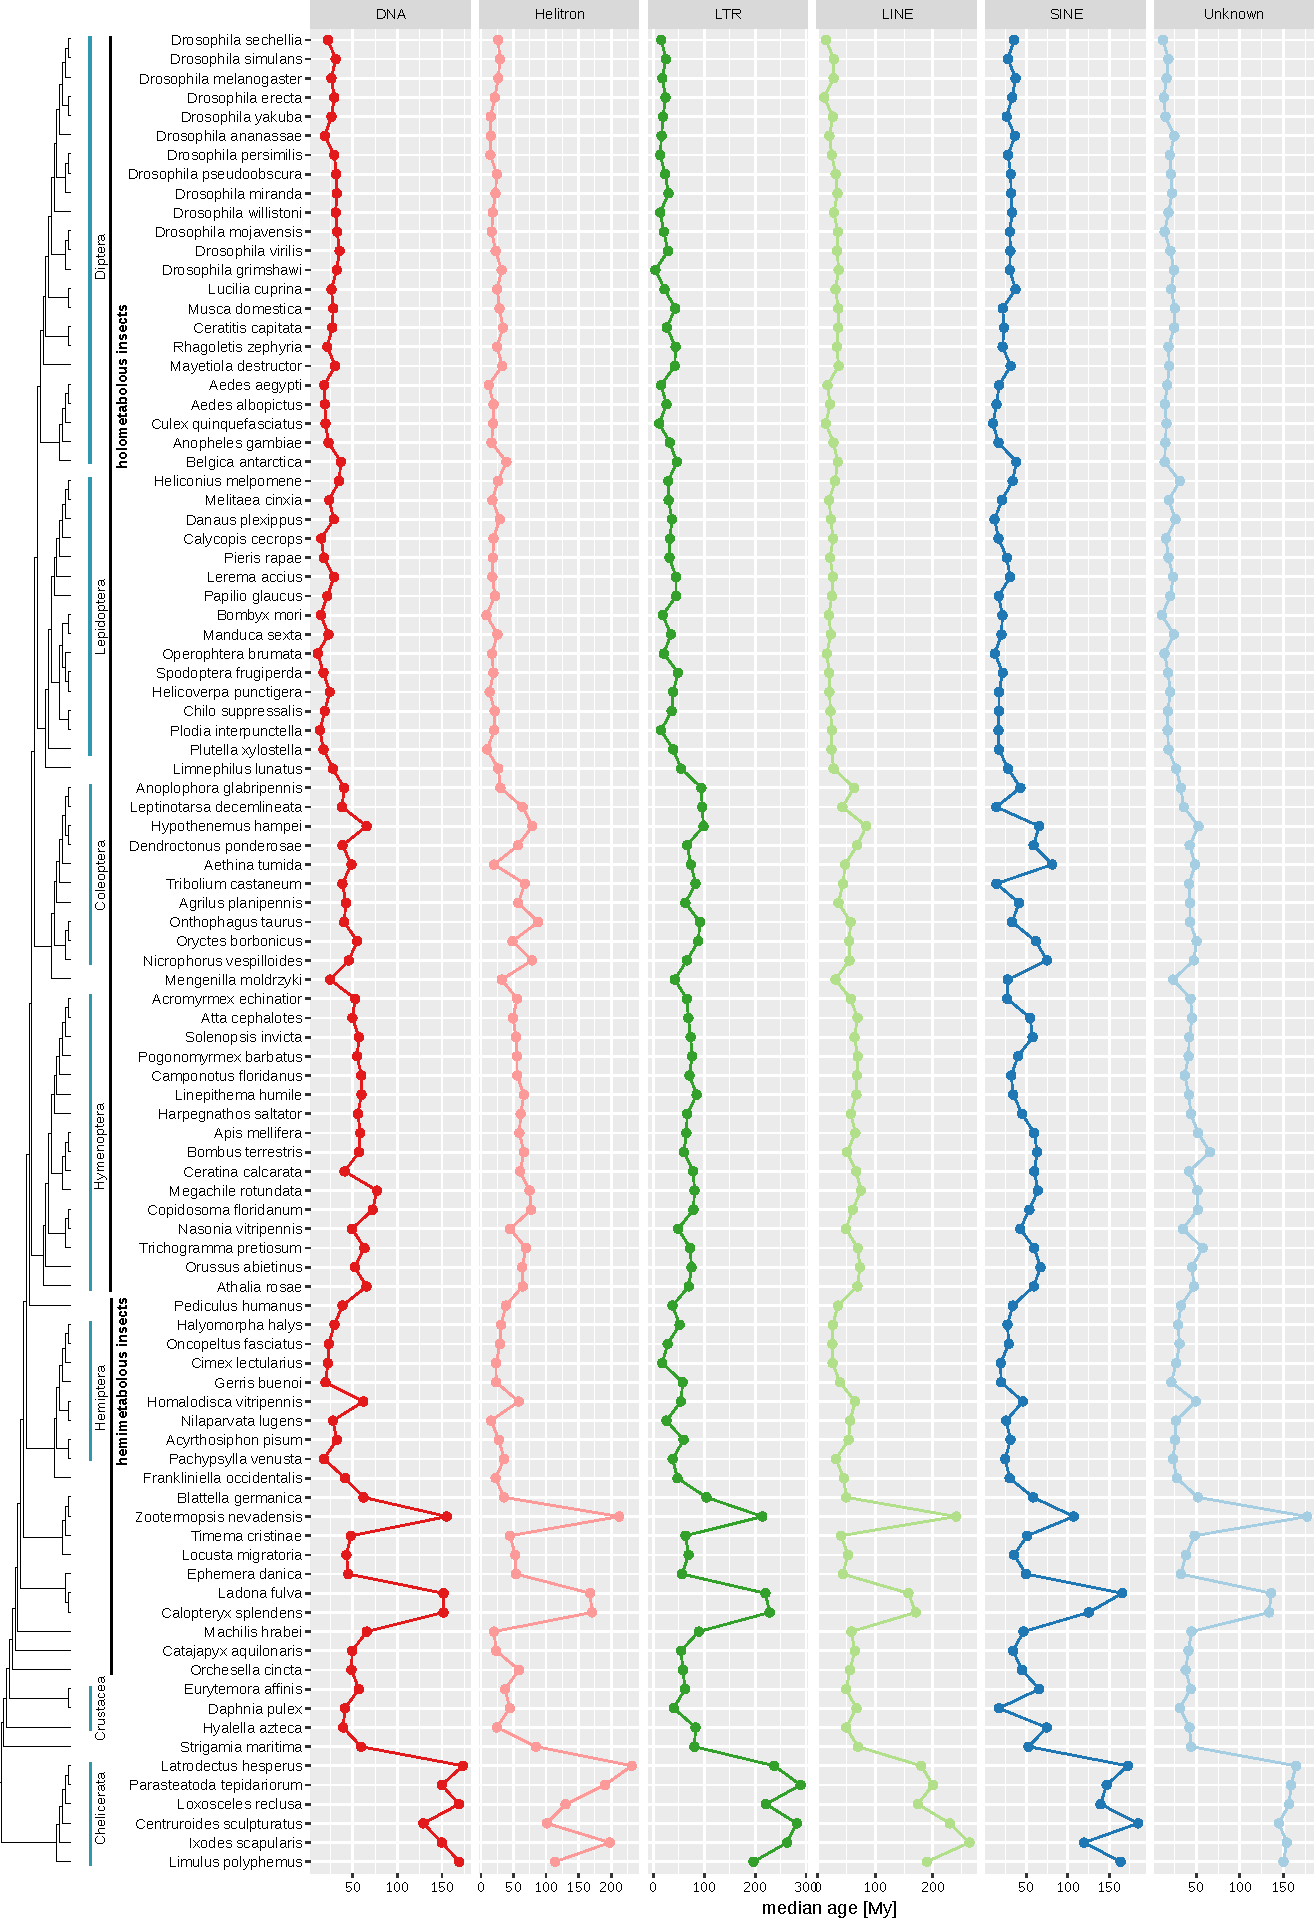
\includegraphics[width=\textwidth]{age-mediane}
\caption[Median ages of TE in arthropods]{{The median ages of six TE subclasses in all sampled species show
variation between and within subclasses. Clade relationships after Misof
et al. (2014). Species relationships within clades are based on the
published phylogenies listed in Table \ref{tab:phylogeny-sources}.
{\label{fig:age-mediane}}%
}}
\end{center}
\end{figure}

\begin{figure}[h!]
\begin{center}
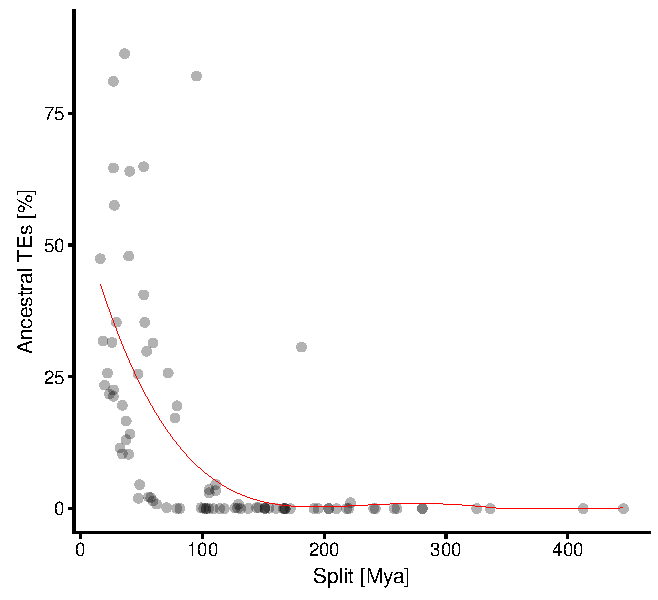
\includegraphics[width=0.70\columnwidth]{age-vs-perc-ancestral}
\caption[TEs are no longer recognized as ``ancient'' beyond a clade age of
\textasciitilde{} 120 Mya]{{TEs are no longer recognized as ``ancient'' beyond a clade age of
\textasciitilde{} 120 Mya. Dots: individual measurements; red line:
polynomial regression. ``Split'' refers to the most recent common
ancestor of the clade and its sister clade.
{\label{fig:age-vs-perc-ancestral}}%
}}
\end{center}
\end{figure}

We inferred the total amount of DNA gained and lost in each lineage by
first calculating the fraction of lineage-specific TE derived DNA,
\emph{i.e.}, the amount of DNA that was gained by TE activity since the
split from its sister species. We subtracted the amount of
lineage-specific TEs (DNA gained since the split of the sister-species
present in our tree) from the assembly size of each species. To compute
the amount of DNA lost, we subtracted the amount of ancestral DNA from
the inferred ancestral genome size of each species. This analysis
revealed highly dynamic genome sizes among species and clades (Figure
\ref{fig:gain-loss} on page \pageref{fig:gain-loss},
Table \ref{tab:gain-loss}). In 75 out of 89 species (we omitted the chelicerates and
myriapods which were not represented in the dated phylogeny), the amount
of DNA loss exceeds the amount of DNA gained through the accumulation of
TEs. These 75 species include five dipterans, in particular two
representatives of \emph{Aedes} mosquitoes, but no representatives of
\emph{Drosophila} or other closely related species. The ratio of gain to
loss ranged between 0.2 in the fly \emph{Rhagoletis zephyria} to 5.1 in
the butterfly \emph{Calycopis cecrops}.

\begin{figure}[h!]
\begin{center}
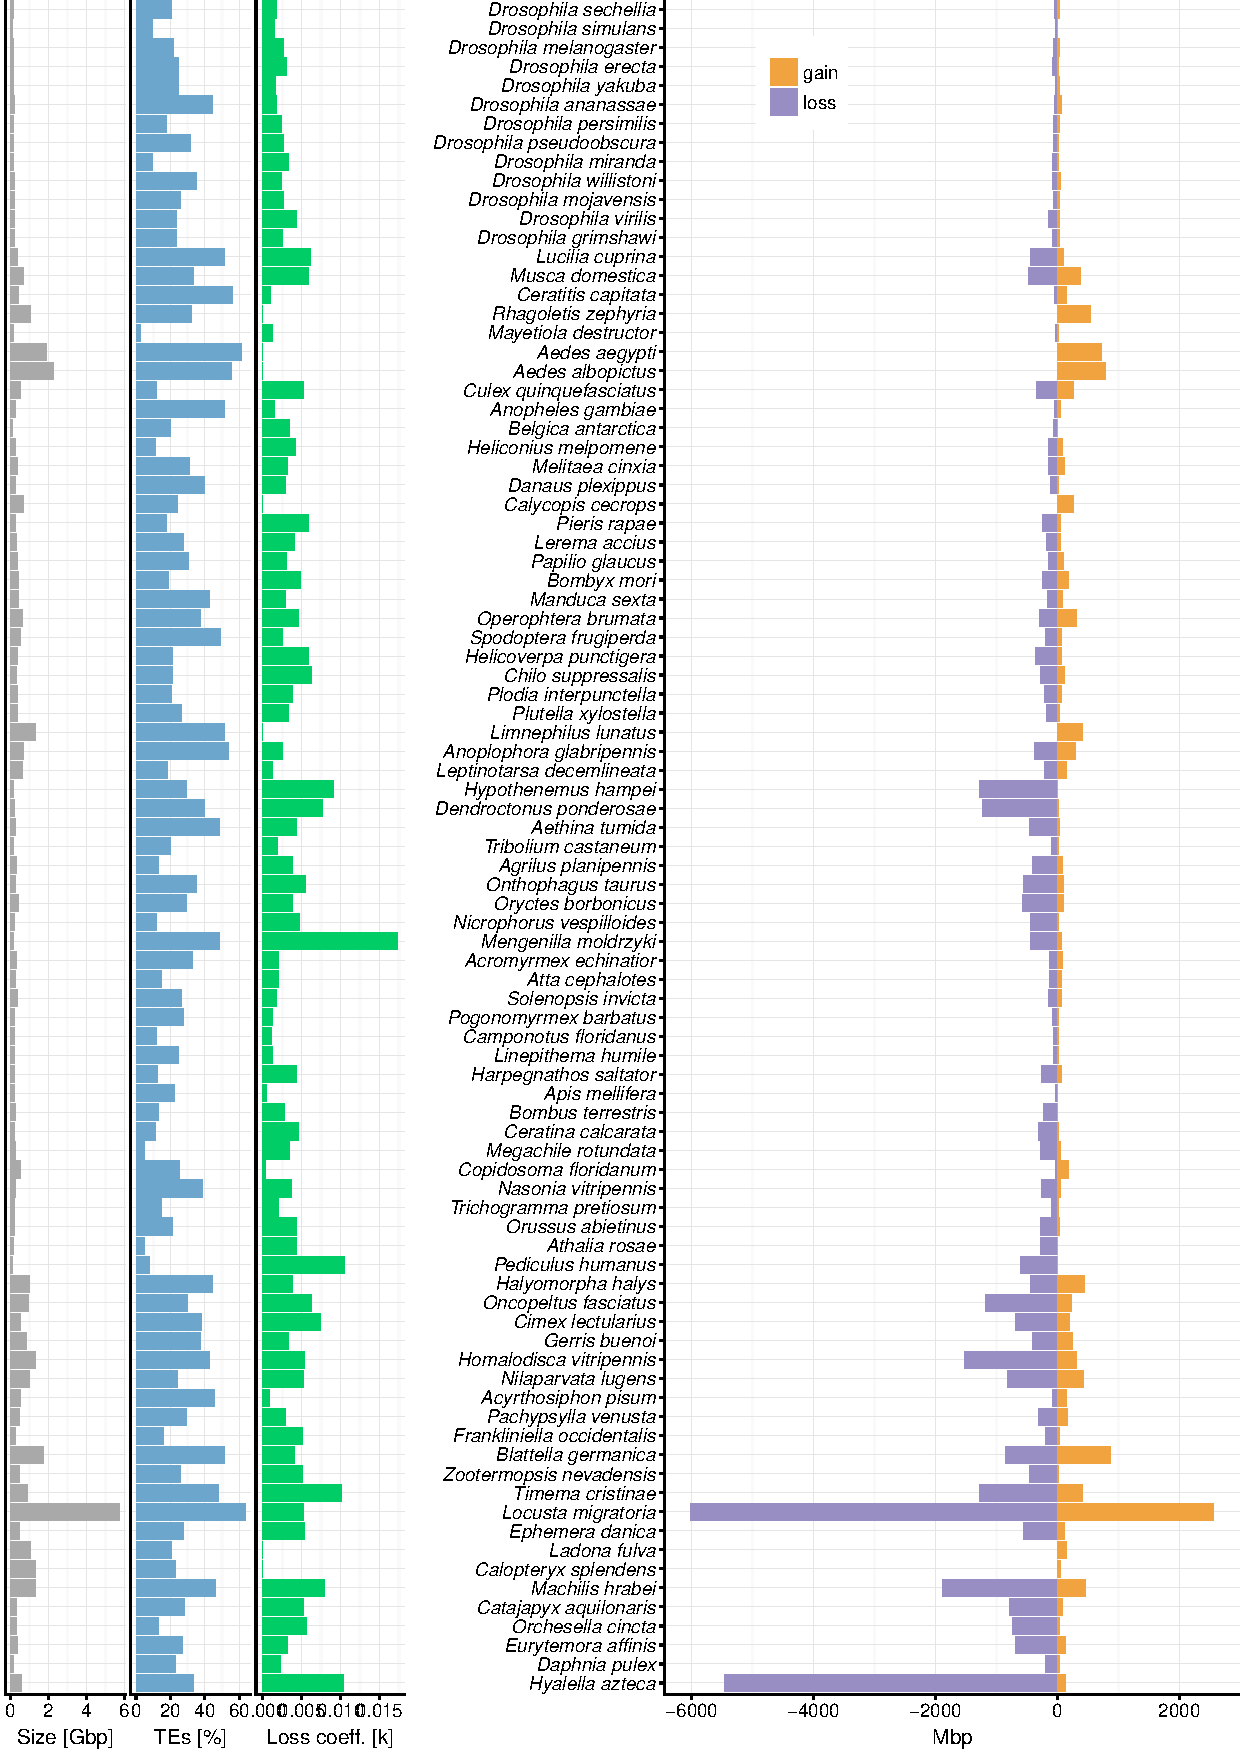
\includegraphics[width=\textwidth]{gain-loss}
\caption[DNA gain and loss rates]{{Increased DNA loss rate explains some of the observed genome size
reductions in insects, but not all. The opposite is true, however: for
species with negative loss coefficients we inferred increased genome
sizes compared to other species in the same order, sometimes drastically
so.
{\label{fig:gain-loss}}%
}}
\end{center}
\end{figure}

We inferred the largest absolute values of DNA gain (3.7 Gbp) and loss
(7.1 Gbp) in the locust \emph{Locusta migratoria} with 5.8 Gbp, the
largest studied genome. It is followed by the amphipod \emph{Hyalella
azteca}, which was inferred to have lost 5.4 Gbp, but gained only 136
Mbp. In general, crustaceans appear to have lost large absolute amounts
of DNA, however the average ratio of DNA gain to DNA loss (0.11) is
estimated to be lower compared to hexapods (0.88). The ratio of DNA gain
to DNA loss was not significantly different in holometabolous and
hemimetabolous insects (phylogenetic ANOVA, \(p = 0.5\)).

With the inferred DNA sequence gains and losses, we calculated the DNA
loss coefficient according to \citet{Kapusta2017a}. The DNA loss
coefficient, \(k\), is calculated from the amount of DNA
gained and lost since the last ancestor (difference between the extant
genome size and the ancestral size in terms of lineage-specific DNA; see
Methods). We assume that the DNA loss coefficient is constant over time
and describes the loss of DNA sequence over time within a genome of a
particular species. It has to be kept in mind that DNA loss is
counterbalanced by DNA gain due to TE propagation within a genome. We
found an extremely high DNA loss coefficient in the strepsipteran
\emph{Mengenilla moldrzyki} with a small genome (156 Mbp, 48.5 \% TEs;
\(k = 0.0173\)). We found the lowest DNA loss coefficients in the
two mosquitoes \emph{A. aegypti} (1,871 Mbp, 61.2 \% TEs,
\(k \approx 0\)) and \emph{A. albopictus} (2,247 Mbp, 55.6 \% TEs,
\(k \approx 0\)), both of which have large genomes and a high TE
content.

Interestingly, genome assembly size and DNA loss coefficient are
negatively correlated (Kendall, PIC, \(p = 0.001\)) in contrast to
a weak positive correlation between TE content and DNA loss coefficient
(Pearson, PIC, \(p = 0.03\)). However, using PIC there is no
correlation at all (Supplemental Figure \ref{fig:loss-coefficient}), neither among all species
nor when subsampling the dataset to Holometabola/Hemimetabola or by
taxonomic order. Instead, genome size appears to remain more or less
constant (albeit with a large spread) despite changing coefficients of
DNA loss. This is in stark contrast to the findings by
\citet{Kapusta2017a} who also reported a negative correlation between DNA
loss coefficient and genome size in birds and mammals, but a significant
positive correlation supported by PIC between TE content and DNA loss
coefficient (Supplemental Figure \ref{fig:te-content-vs-size}).


\section{Discussion}

We present the most comprehensive analysis of genome size dynamics in
arthropods, focusing on gain and loss of TE-derived DNA. In arthropods,
and particularly in hexapods, genome size variation, which reaches an
amplitude of up to 1,600 \% (Figure \ref{fig:tree-with-ancestral-sizes}), which substantially exceeds
variation in mammals and birds \citep{Kapusta2017a}. \citet{Kapusta2017a}
proposed an explanation for the relatively invariant genome sizes within
mammals and birds, which can be observed despite the active propagation
of TEs in these genomes, namely an ``accordion'' model of genome size
evolution. The ``accordion'' model of genome size dynamics assumes that
DNA gain, for example through massive lineage-specific TE propagation,
is counteracted by DNA loss, for example, via ectopic recombination and
other mechanisms and subsequent removal by repair mechanisms. This
process is supposed to maintain a genome size equilibrium.
Mechanistically, the ``accordion'' model proposes that TE insertions
lead to DNA gain, but also generate targets for ectopic recombination
which can induce DNA loss. \citet{Kapusta2017a} further show that there is
empirical evidence in mammalian and bird genomes of frequent
macrodeletions compatible with the action of ectopic recombination.
Given the proposed mechanistic explanation of the ``accordion'' model,
it should also apply to arthropod genomes. In fact, we inferred a
similar balance of DNA loss and gain within the major insect orders:
Large genome sizes are correlated with high TE content (Figure
\ref{fig:te-content-vs-size}) and
high amounts of DNA loss (Figure \ref{fig:loss-coefficient}), but the ``accordion'' model does
not explain the large periodic shifts in genome size between the major
insect orders. Instead, insect genomes appear to cope with TE influx in
an entirely different manner than vertebrate genomes. Where in mammals,
a high rate of DNA loss leads to a smaller extant genome size, in
insects the genome size remains more or less constant (within the large
range of dispersion) according to our DNA loss coefficient inferences
(Figure \ref{fig:loss-coefficient}). These results suggest that in insect genomes, even a high
rate of DNA loss is barely able to cope with the high rate of DNA influx
due to TE activity and and potentially transfection keep the genome size
stable -- we did not observe a stable trend towards genome shrinkage in
insects. However, the ancestral genome size reconstruction suggests that
there have been periods of genome contraction during the evolution of
arthropods which are not modeled using a constant coefficient of DNA
loss. To better infer the pattern of DNA loss over the
\textasciitilde{}450 million years of insect evolution would require a
variable DNA loss coefficient and a model that can take into account
ancestral genome sizes and DNA gain/loss states at multiple points in
the phylogeny.

Genome size reduction in vertebrates has been implicated in the
metabolic requirements of powered flight \citep{Wright2014}; this is
indicated by the fact that birds with higher metabolic rates, such as
hummingbirds, have smaller genomes than flightless birds
\citep{Gregory2005}. In insects, we would expect a similar rate of DNA
removal over time if powered flight should play a role. However, we
observe a different situation: in flightless arthropods, genome size
shows a trend to increase with the DNA loss coefficient, while in
insects capable of flight, the trend is downwards (Figure
\ref{fig:loss-coefficient-plots-flight}). Hence, the
metabolic rate is likely not a predictor of genome size in insects,
regardless of flight capability.

\subsection*{Ancient TEs become
unrecognizable}

We found almost no ancestral TEs in species that diverged earlier than
100 Mya from their sister species (Figure
\ref{fig:age-vs-perc-ancestral}). This is most likely a
consequence of the TE nucleotide sequence similarity decaying over time
and thus sequence homology becoming undetectable. Its effect is easily
visualized when plotting the TE content distribution over the sequence
divergence (or age, if conversion is available) and dividing the
landscape in two parts, separated at the age of the species (Figure
\ref{fig:ancient-lineage-specific}).
These findings are in line with other studies suggesting that inactive
TEs become unrecognizable beyond 50 Mya due to high sequence divergence
(\emph{e.g.}, SINES \citep{Shedlock2000}).

\subsection*{Genome contraction covaries with TE
expansion}

Insects have much larger effective population sizes than mammals or
birds, which limits the effects of genetic drift and exacerbates the
efficiency of natural and purifying selection \citep{Szitenberg2016}. As a
result, we would expect TE activity to both be of limited detrimental
effect to the host organism, and lead to widely distributed copies of
active TEs among the individuals of a population. The latter can happen
within a few generations, as has been shown in \emph{Drosophila} fruit
flies \citep{Kofler2015}; our analysis suggest a similar rate of
intra-population TE proliferation in other insect species, however this
remains to be tested experimentally.

TE activity has been shown to be a pivotal agent shaping genome size
evolution in insects \citep{Maumus2015}, with DNA loss barely
counteracting DNA gained by TE transposition to maintain a genome size
equilibrium. For example, the large genome of the migratory locust
\emph{Locusta migratoria}, which consists of over 60 \% TEs, exhibits a
moderate rate of DNA loss (DNA loss coefficient of \emph{k} = 0.003),
which did not prevent it from being inflated over time due to TE
proliferation. On the other hand, there are examples to the contrary,
documenting that a high rate of DNA loss can lead to small genomes
despite high TE content; this is the case in \emph{Mengenilla
moldrzyki}. In these species, it appears that DNA loss is more efficient
at keeping overly high TE activity in check. However, these traits
appear lineage-specific and cannot be generalized to other
representatives of the same orders.

\subsection*{Limitations of the methods in insect
genomes}

This analysis is of course heavily influenced by the node dating of the
underlying phylogeny, and our approach using COI barcode sequences
cannot rival the accuracy of phylogenomic studies (\emph{e.g.},
\citet{Misof2014}). However, using calibration points from
\citet{Misof2014} enabled us to estimate node ages with reasonable
accuracy and therefore provide a robust dated phylogeny for the TE age
classification. Unfortunately, for some species there were no closely
related species in the dataset, which forced us to select an ancestral
split that is older than the species would be. This was the case for all
orders with only a single representative (Collembola, Diplura, Psocodea,
Trichoptera, and Mecoptera). Here, the representative species were
assigned an age that is even older than the age of the sister order,
which likely led to an underestimation of the ancestral TE content. To
solve this issue, genome size estimates for more representatives of
these orders are required. This also highlights the importance of
efforts like the genome size database \citep{Gregory2018} in the age of
whole-genome sequencing -- not only because the estimates aid in
establishing sequencing strategies, but also for comparative analyses
like this one.

\citet{Kapusta2017a} obtained a dataset that included a multiple whole
genome alignment of 100 vertebrate species. Using this whole genome
alignment, they were able to infer micro- and macrodeletions in the
vertebrate lineage. These are lacking in our dataset simply because
whole genome alignments are difficult in insects due to low conservation
of synteny: while the human genome aligns with over 98 \% to the
chimpanzee genome and with around 70 \% to the mouse genome
\citep{Mural2002} this is not the case in insects across larger
evolutionary time scales. For example, the honey bee \emph{A. mellifera}
genome aligns to less than 20 \% of the turnip sawfly \emph{Athalia
rosae} genome, also a representative of the order Hymenoptera (A.
Donath, \emph{pers. comm}). Thus, we omitted analysis of micro- and
macrodeletions and segmental duplications in the insect genomes.
However, since these events make up at most 10 \% of the vertebrate DNA
gain or loss \citep{Kapusta2017a}, with the analysis on TEs we have
covered the major source of DNA gain and loss in arthropod genomes. Our
analysis is instead based on a wider dataset with twice as many species
from all major insect and crustacean orders. This provided us with a
broad comparative view on genome size dynamics in arthropods.

\section{Conclusion}

We show that genome size in insects is governed by complex dynamics that
are not entirely explained by TE activity alone. There are large-scale
differences even between (relatively) closely related taxa. We find that
the ``accordion'' model that describes DNA gain and loss in birds and
mammals \citep{Kapusta2017a} does not fit the DNA gain/loss dynamics in
insect genomes. Instead, we find that DNA loss does not counteract TE
proliferation: on average, the genome size remains more or less stable
despite large amounts of DNA lost.


\addcontentsline{toc}{section}{References}
\bibliographystyle{apalike2}
\bibliography{references}

%!TEX root = ../dissertation.tex
\chapter{Orthograph: Mapping coding nucleotide sequences to clusters of
orthologous genes}
\label{cha:orthograph}

\hyphenation{HaMStR pHMMs or-tho-lo-gy pa-ra-me-ters al-go-rith-mic}

\newpage

This chapter has been published in: Petersen, M., Meusemann, K., Donath, A.,
Dowling, D., Liu, S., Peters, R.S., Podsiadlowski, L., Vasilikopoulos, A.,
Zhou, X., Misof, B., Niehuis, O. (2017). Orthograph: a versatile tool for
mapping coding nucleotide sequences to clusters of orthologous genes. \emph{BMC
Bioinformatics}, 18, 111.
doi:\href{https://dx.doi.org/10.1186/s12859-017-1529-8}{10.1186/s12859-017-1529-8}

\bibentry{Petersen2017}

Author contributions to the original article:\\
MP, BM, and ON conceived the Orthograph algorithm. MP wrote the
Orthograph software. ON, AV, AD, BM, and KM contributed with suggestions,
code review, and helper scripts to the Orthograph package. MP, KM, AD, DD,
SL, RSP, LP, XZ, and ON contributed to the apoid wasp transcriptomics. MP,
BM, and ON wrote the manuscript.

\section{Background}

Inferring the evolution of gene families, the phylogeny of species, and
tracing the biogeography of populations depend on reliable delineation
of orthologous genes and paralogous copies of them. While delineation
and identification of orthologous and paralogous genes has been firmly
established for studying genomic data (reviewed by \citep{Kristensen2011}
and benchmarked by \citep{Trachana2011}), few approaches are currently
available for assessing transcripts in the same manner (proposed by,
\emph{e.g.}, \citep{Ebersberger2009} and \citep{Schreiber2009}). Each of
these approaches exhibits, and suffers from, specific problems,
potentially leading to erroneous species and gene tree inference (see
below). We developed a novel software pipeline, called Orthograph, for
convenient, fast, and reliable identification of orthologous (and
paralogous) nucleotide or amino acid sequences, which resolves existing
algorithmic and software-technical issues. Orthograph builds on
previously proposed graph-based clustering algorithms, but extends them
without sacrificing accuracy or computational speed.

When comparing the gene repertoires of species, one of the first
analytical steps is the delineation of orthologous genes
(\emph{orthologs}), \emph{i.e.}, the identification of genes that
originated from a single gene in the last common ancestor of the
compared species. Each of the delineated orthologous groups (OGs) can
also include species- or lineage-specific gene copies
(\emph{inparalogs}), that evolved by gene duplication after the
evolutionary split of the ancestor into different species
\citep{Koonin2005}. Finally, horizontal gene transfer can give rise to
xenologous gene copies (\emph{xenologs}) from a single ancestral gene
\citep{Koonin2005}.

Two fundamentally different approaches to identify potential orthologs,
paralogs, and xenologs have been established: tree-based and graph-based
approaches. The benefit of graph-based approaches, which we will
subsequently focus on, is their computational efficiency and scalability
(for reviews and a comprehensive discussion of the benefits of the
different approaches, see \citep{Dutilh2007} or \citep{Kristensen2011}).
In general, graph-based approaches assessing gene orthology make use of
the genome-wide best reciprocal hit (BRH) criterion. It rests on the
assumption that orthologs in two genomes are more similar to each other
than to any other gene in the compared genomes, since they are direct
and exclusive descendants from a single ancestral gene
\citep{Altenhoff2012}.

Various graph-based approaches based on the BRH criterion have been
developed that \emph{de novo} infer orthology among genes and proteins
in the gene or protein sets of sequenced and annotated organisms, such
as OrthoMCL \citep{Li2003}, COCO-CL \citep{Jothi2006}, OrthoDB
\citep{Kriventseva2015}, InParanoid \citep{Sonnhammer2015}, OrthoFinder
\citep{Emms2015}, and OMA \citep{Altenhoff2015}. The reliability of these
methods critically depend on the fact that differential gene loss is the
exception and that gene or protein repertoires are complete. This means
that in order to apply a graph-based approach to infer gene orthology
among genomes, the organisms' gene or protein repertoire must be
reliably known. These methods are therefore not appropriate for
assessing orthology among nucleotide sequences in sequenced
transcriptomes, since transcript libraries contain only a subset of the
organisms' actual gene repertoire. The nucleotide sequence of a gene may
be missing in a given transcript library simply because the gene was not
(sufficiently highly) expressed at the time of RNA preservation. Given
that transcriptome sequencing represents an extremely valuable and
cost-efficient strategy to sample coding nucleotide sequences of a large
fraction of an organism's gene repertoire \citep{Misof2014}, several
graph-based approaches have been developed that are dedicated to
ortholog identification in transcript libraries.

A possible solution to the aforementioned problem in transcript
orthology assessment is to assign transcripts to OGs whose genealogical
relationships have already been reliably inferred, rather than to infer
orthology of these genes \emph{de novo} from the transcripts. Knowledge
of the genealogical relationships of genes can be derived from
comparative genomic analyses and may be retrievable from public
databases such as OrthoDB \citep{Kriventseva2015}. This approach has been
implemented in OrthoSelect \citep{Schreiber2009} and HaMStR
\citep{Ebersberger2009}. However, OrthoSelect does not implement the BRH
criterion, but a unidirectional search. OrthoSelect is thus prone to
false positives. HaMStR, on the other hand is more sophisticated since
it applies a BRH orthology prediction strategy. Specifically, HaMStR
uses profile hidden Markov models (pHMMs) that represent properties of
the aligned amino acid sequences of each known OG to search a transcript
library on the amino acid level for matches. All retrieved hits are then
searched against the entire set of proteins, \emph{i.e.}, the proteome
(also referred to as ``official gene set'') as reference gene set (RGS),
of each of the species of which amino acid sequences were used to
construct the pHMM. If this reciprocal search retrieves the same amino
acid sequence(s) that was (were) used in the construction of the pHMM, a
the respective transcript is mapped to the OG in question.

The algorithm of HaMStR is ``memoryless'', meaning that during
evaluation of the BRH criterion for a given OG, it does not consider
which transcripts have been assigned to other OGs. Since transcripts are
assigned to OGs on a per-OG basis without considering results from
evaluations for other OGs and keeping track of what transcripts have
already been assigned, it is possible that a given transcript is mapped
to more than one gene. This issue of redundant transcript assignments
can result in a misled inference of phylogenetic relationships, as has
been shown \citep{Struck2011,Kvist2013}, and can potentially compromise
downstream analyses. In HaMStR, it would be conceivable to prevent
redundant transcript assignment by implementing a record of previously
assigned transcripts. However, such a first-come-first-serve approach
cannot be justified: transcripts must be assigned to the OG that they
are most likely orthologous to, not to the OG that came first in the
search order. Since this serious issue cannot be solved using the HaMStR
algorithm, we developed Orthograph: a different algorithm that
circumvents redundant transcript assignments and instead maps
transcripts to the globally best matching OG.

To assess the sensitivity and accuracy of Orthograph, we tested whether
or not Orthograph a) reliably identifies orthologs, b) detects known
paralogs, and c) finds known isoforms or alternative transcripts. We
additionally searched 24 \emph{de novo}-sequenced transcript libraries
of apoid wasps for 5,561 orthologous genes to assess the computational
performance of Orthograph. Finally, we verified that Orthograph does not
map transcripts to more than one gene by re-analyzing a dataset that has
been processed with HaMStR. Our results demonstrate that Orthograph's
performance is on par with HaMStR's while not suffering from redundant
transcript assignment. Further, we emphasize the flexibility of
Orthograph and highlight features that are likely of particular interest
for a wide array of analyses in molecular evolutionary biology and in
	comparative genomics in particular.

\section{Implementation}

The Orthograph software package is divided into three main tools that
handle (i) database management (manager), (ii) forward and reverse
searches (analyzer), and (iii) clustering of orthologous transcripts and
output (reporter). The separation into three distinct tools is a
deliberate design choice to address work environments where users do not
have full administrative privileges. This facilitates implementation in
a high-performance computing cluster setup where the administrator can
use the appropriate tool to manage the database, while users only need
to run the actual analysis tools. In addition, this design allows the
user to evaluate the alignment search results using different settings
(\emph{e.g.}, different alignment bit score thresholds to fine-tune and
optimize parameters) quickly without re-running the computationally
expensive searches.

Orthograph builds on the transcript orthology assessment strategy via
BRH suggested by \citep{Ebersberger2009}. In contrast to the
implementation of this strategy in HaMStR, Orthograph assigns a given
transcript to the \emph{globally} best matching OGs while making sure
that no transcript is assigned more than once. It additionally
identifies all transcripts (splice variants and inparalogs) present in
an assembled transcript library that are putatively homologous to a
given OG. The specific transcript orthology assignment algorithm is as
follows (Figure \ref{fig:orthograph-workflow} on page
\pageref{fig:orthograph-workflow}); note that steps 1 through 3 are only
required once since their output can be used for all subsequent
analyses:

\begin{enumerate}
\item
  The proteomes (``reference gene sets'', RGS) of reference species are
  used as input.
\item
  Orthologous genes from all reference proteomes are clustered to form
  orthologous groups (OGs). This information is provided from public
  databases or one's own orthology delineation in the RGS.
\item
  For each OG, the amino acid sequences are aligned and the multiple
  sequence alignment (MSA) is used to construct a profile HMM.
\item
  These pHMMs are used to search the transcript sequences on the amino
  acid level for candidate homologs.
\item
  Search results are stored in a relational database.
\item
  For each pHMM search hit, the target amino acid sequence section
  matching the pHMM is used as a query to search in a database that
  includes all genes from the RGS (including the genes that form OGs) on
  the amino acid level.
\item
  The results of the reverse search are also stored in the relational
  database.
\item
  After all forward and reverse searches have completed, the clustering
  of BRH pairs takes place: search results from all forward searches are
  sorted by descending alignment bit score. For each forward alignment
  search result, the corresponding reverse alignment search results are
  sorted by descending alignment bit score as well. They are evaluated
  in order of descending alignment bit score for the forward search
  results, starting with the highest alignment bit score.
\item
  If the best reverse search hit of a given transcript is part of the OG
  that the pHMM for the forward search is based on (\emph{i.e.}, the BRH
  criterion is fulfilled), the target transcript is assigned to the OG.
  The target transcript section is marked so that it cannot be assigned
  again. Each entry in the database is evaluated in this manner.
\end{enumerate}

Orthograph performs several post-processing steps on transcripts
assigned to OGs. By aligning the transcript fulfilling the BRH criterion
to the most similar orthologous amino acid sequence of a reference
species using Exonerate \citep{Slater2005}, it infers a
frameshift-corrected open reading frame (ORF). Orthograph allows to
extend the ORF beyond the pHMM alignment sequence section for which the
BRH criterion was fulfilled while making sure that the orthologous
region is covered by a user-defined percentage of the ORF length.
Subsequently, it provides both the amino acid sequence and the exactly
corresponding frameshift-corrected nucleotide sequence of a given
transcript. Additionally, Orthograph can concatenate transcripts of a
given OG to simplify downstream analyses (\emph{e.g.}, phylogenomic
investigations). In all above analysis steps, the user can fine-tune all
relevant search and evaluation parameters using configuration files for
clarity, documentation, and reproducibility.

\begin{figure}[t]
\begin{center}
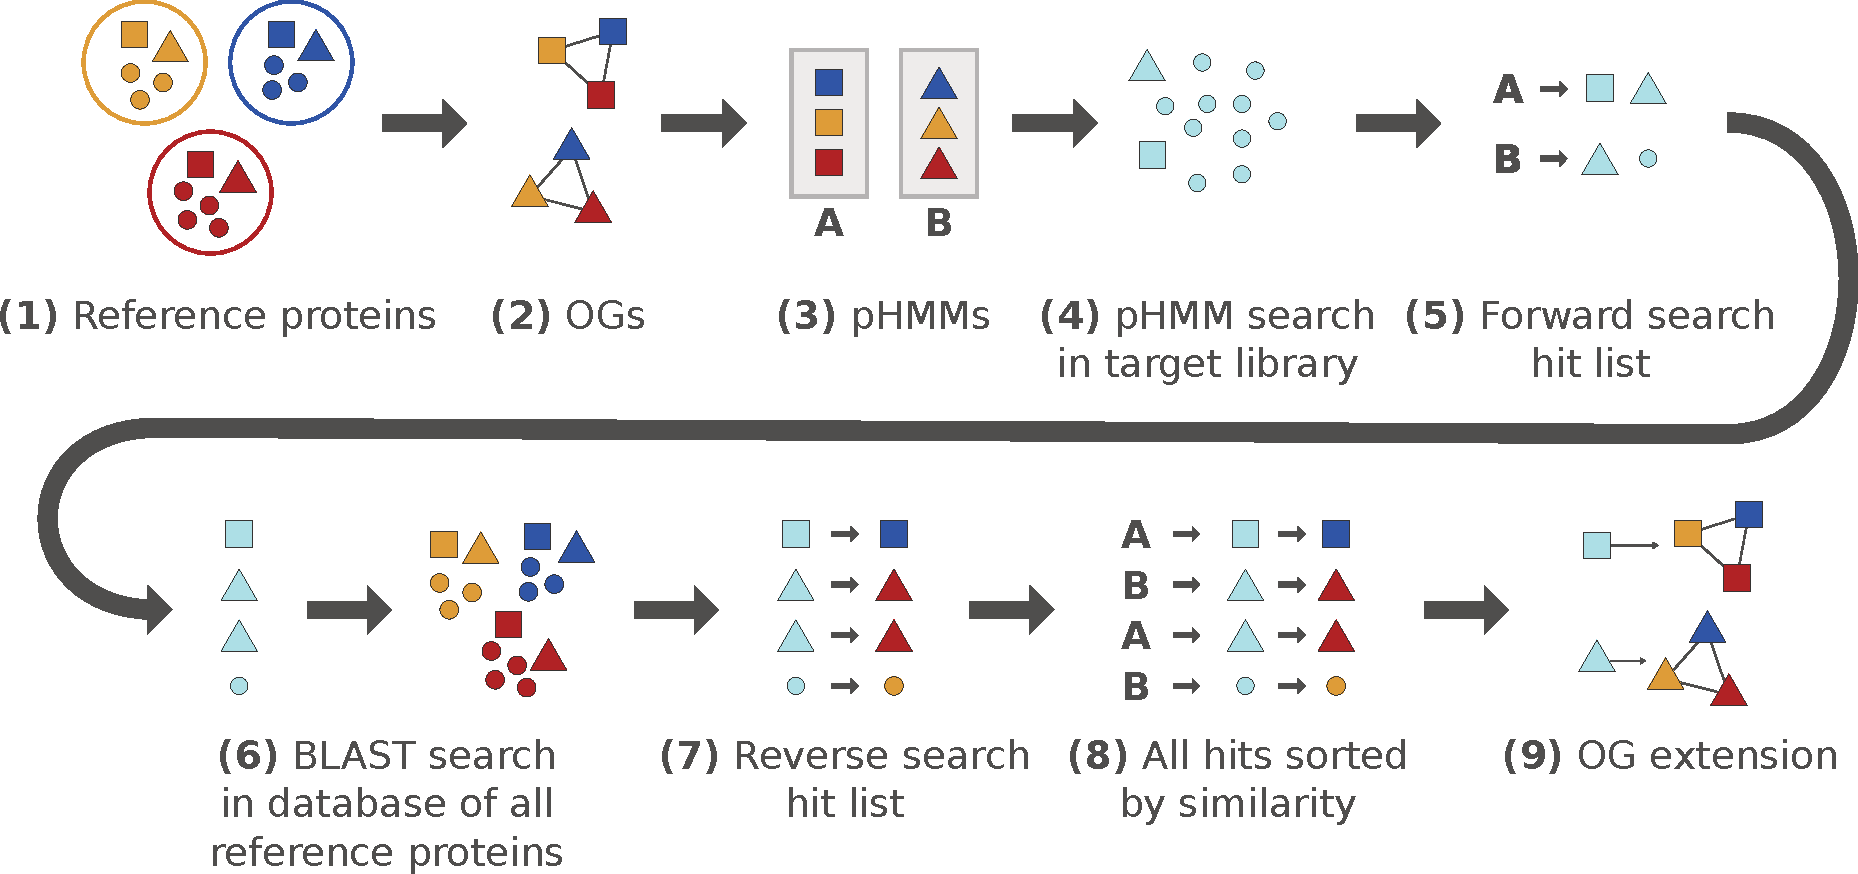
\includegraphics[width=\textwidth]{orthograph-workflow}
\caption[Orthograph workflow]{Orthograph workflow. From a set of
reference proteins (1), the proteins are clustered to form orthologous groups
(OGs) (2). These OGs are aligned to construct profile hidden Markov models
(pHMMs) (3). The pHMMs are used to search for candidate orthologs in the
target library (4). Each of the obtained hit amino acid sequences (5) is used
as a query for a BLAST search in a database comprising all reference proteins
(including the ones forming OGs) (6). Search results from both forward and
reverse searches (7) are collated and sorted by bit score, with the reverse
search result order being subordinated to the forward result order (8). This
list is evaluated in descending order: if the reverse search hit a protein
that is part of the OG used for the forward search, the candidate ortholog is
mapped to the OG (9).}
\label{fig:orthograph-workflow}
\end{center}
\end{figure}

Orthograph has been developed with user friendliness in mind. As a
result, it is easy to install and runs on any Unix/Linux system
(including OS X) that provides its dependencies (see Materials and
Methods). The generation of custom-tailored ortholog sets, \emph{e.g.},
from public databases is facilitated by its ability to parse simple
tab-delimited tables. Input from public databases such as OrthoDB is
easily formatted accordingly using standard UNIX or spreadsheet tools.
In addition, the Orthograph package contains helper scripts that
simplify the preparation of RGS sequence files for custom-made ortholog
sets as well as summarize results for multiple analyses, \emph{e.g.},
different species or using different settings.

When designing a custom ortholog set, users should pay close attention
to the taxon sampling. Genes that occur in at least two species in each
OG are recommended so that the resulting pHMMs are more informative than
when based on single sequences only. In terms of OG number, there is no
lower or upper bound since the selection depends on the research
question. Orthograph runtime increases linearly with each additional OG.

Detailed methods, data sources as well as system requirements are listed
in the Supplemental Material (Figures
\ref{fig:alignment-regions}-\ref{fig:orthodb-alignments}, Tables
\ref{tab:species}-\ref{tab:1kite-apoid-wasps-accessions}).

\section{Results and discussion}

\subsection{Sensitivity and accuracy when searching for single-copy
orthologs}

To assess the sensitivity and accuracy of Orthograph, we employed it to
identify genes of known orthology in the RGS of the honeybee,
\species{Apis mellifera} (15,314 genes, \citep{Honeybee2006}), and
Jerdon's jumping ant, \species{Harpegnathos saltator} (18,564 genes,
\citep{Bonasio2010}).  Specifically, we searched the RGS for 4,625
protein-coding genes provided by OrthoDB 5 \citep{Waterhouse2011a} as
being single-copy across four species of Hymenoptera (\species{Apis
mellifera} \citep{Honeybee2006}, \species{Camponotus floridanus}
\citep{Bonasio2010}, \species{Harpegnathos saltator} \citep{Bonasio2010},
\species{Nasonia vitripennis} \citep{Werren2010}) and the outgroup beetle
\species{Tribolium castaneum}
\citep{TriboliumGenomeSequencingConsortium2008} (download URLs are listed
in the Supplemental Material, Table \ref{tab:ogs}). Note that we removed all
entries of the respective taxon whose RGS we analyzed for assessing the
sensitivity and accuracy of Orthograph from this ortholog set (resulting
in two sets: one without entries from \species{A. mellifera}, and one
without entries from \species{H.  saltator}). Of the 4,625
protein-coding genes that we searched for, Orthograph identified 4,582
(99.07 \%) in the RGS of \species{A. mellifera} and 4,590 (99.24 \%) in
the RGS of \species{H. saltator} (Table \ref{tab:orthograph-tests} on
page \pageref{tab:orthograph-tests}). In the case of \species{A.
mellifera}, five proteins were assigned to other OGs than they were
assigned by OrthoDB. We found a similar result for three proteins of the
RGS of \species{H. saltator}. Visual inspection of these proteins
suggested that the orthology assignment of these proteins in the OrthoDB
database is not correct (for an in-depth assessment and discussion of an
example see Supplemental Material, Figure \ref{fig:orthodb-alignments}). The low fraction (less
than 1 \%) of non-recalled genes were caused by a comparable effect
(Figure \ref{fig:orthodb-alignments}).  Thus, the sensitivity (true positive rate), defined as the
ratio of true positives to true positives plus false negatives, was
0.9896 for the \species{A. mellifera} RGS and 0.9918 for the \species{H.
saltator} RGS. The accuracy, defined as the ratio of true positives plus
true negatives to the total number of genes in the RGS, was 0.9965 for
the \species{A. mellifera} RGS and 0.9978 for the \species{H. saltator}
RGS.

For comparison, HaMStR v13.2.3 was run on the same datasets with
comparable parameters. HaMStR identified 4,589 genes (99.22 \%) in the
RGS of \species{A. mellifera} (1 false positive) and 4,573 genes (98.88
\%) in the RGS of \species{H. saltator} (2 false positives). This
results in a sensitivity of 0.992 in the \species{A. mellifera} RGS and
of 0.9883 in the \species{H. saltator} RGS, and an accuracy of 0.9975 in
the \species{A.  mellifera} RGS and of 0.9969 in the \species{H.
saltator} RGS.

The input data on ortholog relations were retrieved from OrthoDB which
contains OG information inferred in a purely automated fashion
\citep{Waterhouse2011a}. OrthoDB has been attested low numbers of false
positives and spurious assignments \citep{Trachana2011}; the proportion
of less than 1 \% of the genes that were recalled wrongly by Orthograph
are in line with these benchmarks. Orthograph and HaMStR perform roughly
equally in accuracy and sensitivity when it comes to identifying
single-copy orthologs.


% Please add the following required packages to the document preamble:
% \usepackage{booktabs}
\begin{sidewaystable}[h!]
\caption[Orthograph performance compared to
HaMStR \citep{Ebersberger2009}]{Results from the tests that compare
Orthograph performance to HaMStR \citep{Ebersberger2009}.  Sensitivity
is defined as the ratio of true positives (TP) to TP plus false
negatives (FN). Accuracy is defined as the ratio of TP plus true
negatives (TN) to the total number of genes in the official gene set
(OGS). FP, false positives. Note that the results are meant to
demonstrate equality in performance despite algorithmic
differences.}\label{tab:orthograph-tests}
\begin{tabular}{@{}llrlrrrrrrr@{}}
\toprule
Software   & Test        & Genes  & Species                & OGS       & Found  & TP    & FP & FN & Sens.       & Acc.  \\
\midrule
Orthograph & single-copy & 4,625  & \textit{A. mellifera}  & 15,314    & 4,582  & 4,577 & 5  & 48 & 0.990       & 0.996 \\
Orthograph & single-copy & 4,625  & \textit{H. saltator}   & 18,564    & 4,590  & 4,587 & 3  & 38 & 0.992       & 0.997 \\
HaMStR     & single-copy & 4,625  & \textit{A. mellifera}  & 15,314    & 4,589  & 4,588 & 3  & 39 & 0.992       & 0.997 \\
HaMStR     & single-copy & 4,625  & \textit{H. saltator}   & 18,564    & 4,573  & 4,571 & 2  & 54 & 0.988       & 0.996 \\
Orthograph & isoforms    & 8      & \textit{C. floridanus} & 17,064    & 7      & 7     & 0  & 1  & 0.875       & 0.999 \\
HaMStR     & isoforms    & 8      & \textit{C. floridanus} & 17,064    & 7      & 7     & 0  & 1  & 0.875       & 0.999 \\
Orthograph & inparalogs  & 647    & \textit{A. cephalotes} & 18,093    & 583    & 583   & 0  & 6  & 0.901       & 0.996 \\
\bottomrule
\end{tabular}
\end{sidewaystable}

\subsection{Identification of splice variants or
isoforms}

We used Orthograph to assess orthologous amino acid sequences including
isoforms in the RGS of the Florida carpenter ant, \species{Camponotus
floridanus}, a species whose genes and corresponding proteins are part
of the ortholog set analyzed before (see above). In the \species{C.
floridanus} RGS, eight genes that are part of the ortholog set each
encode an alternative isoform. Orthograph readily assigned the
alternative isoforms of seven of these genes to the correct OGs. In the
remaining gene, however, the amino acid sequence of the isoform that
Orthograph could not find was very short (46 amino acids) in length.
Only 21 of the 46 amino acid sites can be well aligned to the OG and
were identified as BRH. It is possible that amino acid sequences that
are significantly shorter than the majority of the OG are scored poorly
by the pHMM search and/or the subsequent reverse search so that they
eventually do not fulfill the BRH criterion and are not recognized by
Orthograph.

HaMStR, in comparison, also identified all isoforms of seven of the
eight genes correctly. However, it reports them as co-orthologs.
Strictly speaking, this term is only correct when, while searching for
single-copy orthologs, one or more copies of the same gene are
identified. Orthograph, in addition to reporting, provides tabular
output with alignment coordinates, HMM alignment bit scores and e-values
for further statistical analyses.

While it would be highly desirable for users to also obtain information
on the occurrence of different isoforms (or alternative transcripts on
the transcriptional level) in different species, alternative transcripts
are difficult to distinguish from transcripts of inparalogs or from
transcript assembly artifacts without additional information, for
example on the genealogy of the species, whose transcript libraries have
been investigated, and/or on the transcript's expression level. However,
Orthograph provides tabular output files that can facilitate
corresponding downstream analyses. Specifically, the Orthograph output
files inform about a) what transcripts form BRHs with ortholog groups
and b) what transcripts assigned by Orthograph to the same ortholog
group overlap (\emph{i.e.}, partially refer to the same coding sequence)
and could thus represent alternative transcripts (or assembly
artifacts).

\subsubsection{Protein isoforms and splice variants in the reference
ortholog set can lead to systematic errors and false
positives}

The presence of isoforms and splice variants in an RGS dataset can lead
to wrong clustering to OGs and/or false negatives (discarded sequences
that should have been mapped elsewhere). Because it is impossible to
know in advance which isoform of a gene or transcribed gene is present
in a given transcript library, it is likely that a BRH search will fail
if more than one highly similar amino acid sequence are present in the
reference RGSs. This occurs because the best reverse search hit of a
candidate ortholog against the database comprising all proteins in an
RGS may return an isoform of the protein that was not used in the pHMM,
leading to a failure to fulfill the BRH criterion. Therefore, isoforms
should either be removed from RGS databases prior to using them in
Orthograph (or in any reference-based orthology prediction tool, for
that matter), or the OGs should be extended to also include the
isoforms.

\subsection{Identification of
inparalogs}

In order to demonstrate Orthograph's capabilities to detect inparalogous
gene copies, we used it to assess genes that are known to have
inparalogous copies in the RGS of the leafcutter ant, \species{Atta
cephalotes} \citep{Suen2011}. Specifically, we retrieved an ortholog set
from OrthoDB 5 comprising 301 OGs that contain genes that are known to
be single copy in the genomes of \species{A. mellifera}, \species{C.
floridanus}, \species{H. saltator}, \species{N. vitripennis}, and
\species{T.  castaneum}, but are multi-copy genes in \species{A.
cephalotes}. These 301 OGs include altogether 647 single-copy and
multi-copy genes from \species{A. cephalotes}: 273 are duplicated, 18
are triplicated, seven have four copies, two have six copies and one has
seven copies. Orthograph readily assigned 583 of the 647 multi-copy
genes to the correct OG (90.1 \%). Two of the 301 OGs were not assigned,
one of which contained four, the other contained two gene copies. In
both cases, the genes from \species{A. cephalotes} were much shorter
than the remaining genes in the OG (18 \% resp. 19 \% of the average
amino acid sequence length), possibly leading to the respective
transcripts failing to fulfil the BRH criterion in the reverse search
step due to an insufficient alignment length. These edge cases again
highlight the importance of high-quality genome sequencing and
annotation efforts, as they provide the basis for many downstream
analyses, including full-length gene sequences for reference-based
orthology assessment.

\subsection{Non-redundant mapping of
transcripts}

In order to test whether Orthograph indeed does not assign transcripts
to more than one OG, we re-analyzed the dataset published by
\citep{Struck2014}, who used HaMStR version 8 \citep{Ebersberger2009}.
Orthograph assigned transcripts to 1,253 OGs, the same number as
obtained by \citep{Struck2014}. However, Orthograph found transcripts of
the analyzed genes in, on average, slightly more taxa (Orthograph:
28.079, \citep{Struck2014}: 26.699). None of the transcripts was assigned
to more than one OG. In the dataset published by \citep{Struck2014}, 274
transcripts were assigned redundantly, however the orthologous regions
were not overlapping. As \citep{Struck2014} removed a total of 1.3 \% of
their sequences from the dataset due to redundantly assigned
transcripts, Orthograph yielded 1.4 \% more taxa per gene, leading to a
denser data matrix for downstream (phylogenetic) analyses.

\subsection{Computational performance of
Orthograph}

To demonstrate the computational performance of Orthograph, we searched
24 apoid wasp transcriptome assemblies for 5,561 selected OGs (sequence
data are deposited at NCBI GenBank; accession numbers are listed in
Additional file 2). The analysis time when using a single thread
increases linearly with total transcriptome assembly length (Spearman
rank correlation, $S = 326$, $p \ll 0.001$, Supplemental Material,
Figure \ref{fig:runtime-vs-length}). Single-threaded analysis time also increases with the number
of assembled transcripts, showing a linear trend, but no significant
correlation (Spearman rank correlation, $S = 1,430$, $p = 0.069$).

Given that next-generation RNAseq datasets tend to be large and current
comparative genomic investigations analyze hundreds, if not thousands of
genes (\emph{e.g.}, \citep{Misof2014}, \citep{Jarvis2014}, the 1000 plants
initiative (\url{https://sites.google.com/a/ualberta.ca/onekp/})), with
a linear runtime increase Orthograph does not pose a time bottleneck for
current and future large-scale studies such as the numerous
group-specific subprojects of the 1KITE consortium
(\url{http://1kite.org/subprojects.html}). For employment in
high-performance cluster computing environments, Orthograph supports
multi-threading: it offers a linear speedup of about 1x until up to four
threads (Fig. \ref{fig:runtime-speedup}). Orthograph scales well with a speedup of 15 to 80 \%
per additional thread up to 12 threads. Using 16 threads reduces
Orthograph running time to around 11 \% compared to a single-threaded
analysis.

Because most of the data are stored in a relational database on the hard
drive, Orthograph requires only little memory and allows to re-evaluate
stored search results with different parameters, which takes only a
fraction of the original analysis time. In a centralized server-client
setup using the MySQL database backend, the database management overhead
is solely handled by the server, freeing CPU resources for the alignment
searches on the clients. For installation in a grid computing
environment where adding a dedicated database server is not feasible,
the SQLite database backend \citep{Hipp2016} is provided. The file-based
SQLite database system can be applied anywhere thanks to its portable
and performant implementation (and is installed by default in most Linux
distributions and Mac OS X), thus it is the default database backend in
Orthograph.

\subsection{Advantages of graph-based orthology prediction
strategies}

Orthograph uses a graph-based approach, like HaMStR and OrthoSelect as
well as orthology prediction tools that assess orthology among genes in
completely sequenced and annotated genomes, such as OrthoMCL, OrthoDB,
OMA, or InParanoid. In contrast, tree-based orthology prediction
strategies such as TreeFam, Ensembl Compara, or the one implemented in
\citep{Capella-Gutierrez2014}, employ an algorithm that reconciles a
phylogenetic tree topology of a gene or gene set with the topology of
the respective species phylogenetic tree. This requires a) a multiple
sequence alignment (MSA) of a gene's amino acid or nucleotide sequences,
and b) a phylogenetic tree inference. Both steps are not only
computationally expensive, but also introduce additional sources of bias
at each step. The much reduced computational complexity of a
bidirectional alignment search compared to a phylogenetic tree inference
enables Orthograph to run on standard workstation computers without
necessitating a high-performance computing environment. A number of
graph-based and tree-based orthology assessment methods have been
reviewed by \citep{Trachana2011}.

\subsection{Reference-based orthology search accuracy depends on
reference database
quality}

Reference-based algorithms for assessing transcript orthology can only
be as accurate as the content of the database providing reference OGs.
The results from testing the performance of Orthograph affirm that
reference-based orthology prediction requires adequate orthology
delineation in reference genomes. These findings further highlight the
necessity for reliable identification of ortholog relations in
completely sequenced genomes as well as continuously updated databases
such as OrthoDB that lay the foundation for a plethora of downstream
comparative analyses. In order to provide comprehensive information,
these databases require high-quality genomic data as well as reliable
structural and functional gene annotation; thus, the importance of
continued genome sequencing and rigorous annotation efforts must not be
underestimated. Likewise, many assembled (draft) genomes are far from
complete in terms of having properly identified their \emph{actual} gene
content \citep{Denton2014}, which also hinders reliable inference of
orthology among them.

\subsection{Reciprocal search by using HMMER and
BLAST}

Orthograph makes use of both pHMM-based and BLAST search technology. By
combining these two fundamentally different alignment search algorithms,
it draws considerable sensitivity and accuracy. Profile HMM-based
similarity searches have been shown to be more sensitive than BLAST when
it comes to detecting remotely related sequences \citep{Eddy2011}. By
restricting the reverse BLAST search to only the (sub)sequence that was
found to be putatively homologous during the pHMM search, the BLAST
query becomes more informative. Therefore, the practice of using BLAST
for the reverse search in Orthograph improves confidence in the
subsequent orthology hypothesis by applying a conservative search
criterion. For an illustration of the interrelations between the search
results and their respective subsequences, see Supplemental Material,
Figures \ref{fig:alignment-regions} and \ref{fig:orf-overlap}.

BLAST uses a heuristic algorithm and does not guarantee an optimal local
alignment. To also support a non-heuristic Smith-Waterman algorithm, we
have, in addition to BLAST, implemented SWIPE \citep{Rognes2011}, which
is also used in OrthoDB. SWIPE uses a BLAST database, thus the BLAST
package is required to generate the database; however the SWIPE search
algorithm does not result in inconsistencies that are possible with
BLAST's alignment heuristic. Users can opt to use the SWIPE algorithm
with appropriate configuration settings.

\subsection{Limits of the methods}

Orthograph is intended to map transcripts of a single species to
reference OGs. Orthology or paralogy relations between genes of more
than one species cannot be established using transcriptomic datasets as
they are inherently incomplete. For assessing orthology among genes in
completely sequenced and annotated genomes, specialized tools exist,
such as OrthoMCL \citep{Li2003}, InParanoid \citep{Sonnhammer2015}, or the
OrthoDB toolset, which is now public \citep{Kriventseva2015}.
Additionally, alternative transcripts or splice variants are difficult
to distinguish in a \emph{de novo} transcriptome assembly without
additional read coverage data, which is why Orthograph refrains from
explicitly predicting them. Orthograph does, however, report transcripts
that are potential alternative transcripts or splice variants in order
to allow researchers to further investigate them.

\section{Conclusion}

With Orthograph, we provide a software solution to accurately assign
transcripts (and other coding sequences) to known groups (clusters) of
orthologous genes (OGs). Orthograph maps transcripts to the globally
best matching OG, circumventing the problem of redundantly assigning
transcripts to more than one OG. With its specific algorithm, Orthograph
solves this issue that earlier implementations of graph-based BRH
mapping strategies suffered from, while maintaining the high sensitivity
and accuracy of the BRH approach. We developed Orthograph to be an asset
in many fields by offering additional functionality compared to earlier
implementations of graph-based BRH mapping strategies. Orthograph is
easy to install and use and thereby facilitates comparative analyses of
transcriptomic and other coding sequence data. It was furthermore
designed to point users to possibly existing alternative transcripts and
paralogous genes, thereby significantly broadening the scope of the
software. The wide applicability of Orthograph has been demonstrated by
its application in a phylogenomic study on apoid wasps using target DNA
sequencing baits \citep{Mayer2016} and the numerous subprojects of the
international 1KITE project, which investigate intraordinal phylogenetic
relationships of insects. Orthograph provides researchers with a
convenient, performant, general-purpose tool for analyses in a plethora
of disciplines in evolutionary biology.

\addcontentsline{toc}{section}{References}
\bibliographystyle{apalike2}
\bibliography{references}

%!TEX root = ../dissertation.tex
\chapter{General Conclusion}
\label{conclusion}

The present thesis comprises research using a multitude of approaches
from comparative genomics, ancestral reconstruction, phylogenetics, as
well as algorithm design and implementation. By using a standardized TE
annotation and a large taxon sampling that encompasses representatives
from all major insect orders, it is able to draw conclusions that
surpass inferences from intra-ordinal comparisons. Additionally, the
development of a new software tool enables researchers to easily assess
orthology within coding nucleotide data.

The software Orthograph (chapter \ref{cha:orthograph} has proven to be a
valuable asset which was used in a number of publications. Many of these
aim to resolve order-level or family-level phylogenies from
transcriptomic data (\eg, Hymenoptera: Vespidae \citep{Bank2017},
Hymenoptera \citep{Peters2017}, Diptera: Acroceridae \citep{Gillung2018},
Hemiptera \citep{Johnson2018}, Diptera \citep{Kutty2018}, Palaeoptera
\citep{Simon2018}). In other publications, it was used to map target
enrichment data to the correct genes \citep{Mayer2016, Sann2018,
Shin2018}, often also for phylogenetic analyses. However, Orthograph was
designed to be versatile, and this shows in its application in studies
that investigate the evolution of specific gene families
\citep{Pauli2016, Dowling2017} or the distribution of DNA methylation in
insects \citep{Provataris2018}. Orthograph was reviewed in
\citet{Nichio2017} and has recieved critical acclaim.

By providing, with Orthograph, a powerful and easy to use tool to
identify orthologs in coding nucleotide data, the efforts described in
chapter \ref{cha:orthograph} facilitate future phylogenetic analyses.
The growing amount of available transcriptomic data for more and more
species enables researchers to further resolve phylogenies based on
molecular datasets with increasing resolution and accuracy. Although for
many species, molecular data will never be obtained (see page
\pageref{mass-extinction}), our understanding of the remaining species'
relationships will develop. This endeavor continues to be important
since all studies dealing with aspects of evolution --- also the ones in
this thesis --- necessitate a concept of species interrelationships.
Thus, Orthograph contributes to furthering the field of biological
(molecular) systematics, which in turn enables other fields such as
evolutionary biology or comparative genomics to make meaningful
inferences.

The focus of the empirical comparative studies in this thesis was on
insect genomes. Insects are very different from vertebrates, plants,
and fungi in both phenotype and genotype. This is also reflected in the
processes that define their genome size with respect to the TE content.
As in vertebrates, TE content is a predictor for genome size, however,
DNA gain and loss rates do not affect genome size in insects as much as
they do in vertebrates \citep{Kapusta2017-1, Lindblad-Toh2005}.
Nevertheless, insect genome size does exhibit large fluctuations
\citep{Alfsnes2017}, but these cannot be explained by differential TE
activity alone.  Similarly, the patterns of DNA methylation, which has
been hypothesized to be involved in TE defense mechanisms, in insect
genomes are drastically different from what has been observed in
vertebrates or plants \citep{Provataris2018, Suzuki2008}. Apparently,
insects do not rely on DNA methylation to inhibit TE proliferation and
thereby genome size expansion. What else, then, could explain the large
spread in insect genome size?

The answer to that question is likely not straigthforward, and the
present thesis does not have it. It does, however, provide a broad array
of pointers for future research. For example, the RNA interference
pathway genes were implicated in TE inhibition \citep{Aravin2001,
Czech2008} and are absent in some butterfly species that exhibited high
TE content \citep{Dowling2017}. The large number of publicly available
lepidopteran genomes provides ample opportunity to closely investigate
these genes and shed more light on TE defense mechanisms. Incorporating
some of these genomes, the study in chapter \ref{cha:mobilome}
characterizes the TE repertoire of 73 arthropod species, the largest
taxon sampling for a comparative study on TE diversity in arthropods to
date. The TE annotation data that were generated for the study are
valuable as a resource to investigate the interaction of TEs with other
genome components such as protein-coding genes. The annotation results
from six insect species \todo{how many did Jeanne use?} were used in
investigations on the protein-coding gene repertoire in insects
\todo{how to cite Jeanne?}. Another part of the TE annotation data was
used by \citep{Provataris2018}, and the annotation pipeline was used to
identify TEs in additional insect genomes. The annotation procedure is
largely identical to the one used by \citet{Reinar2016} who benchmarked
the approach and showed it to be accurate and efficient. By combining
several well-established algorithm implementations into an easy to use
and fully automated pipeline, the shell script provides a tool to
reliably annotate TEs in assembled genomes of non-model species. 

The construction of a dated phylogeny for over 600 insect and arthropod
species from the literature and publicly available DNA barcode data is
unprecendented (chapter \ref{cha:dynamics}). This phylogeny will be
valuable to researchers in many disciplines because it allows to set
insights from other studies into context with the evolution of genome
size in insects.  In fact, the phylogeny also allows to map other
phenotypic characters and to infer ancestral states for them, which is
often a means to study and understand their evolution.

Also in chapter \ref{cha:dynamics}, I inferred ancestral genome sizes
for 613 arthropod taxa including 520 insect species using that dated
phylogeny and likewise publicly available genome size data
\citep{Gregory2018}. While other studies have also exploited this
database to set extant insect genome size into context with other
phenotypic traits \citep{Alfsnes2017, Gregory2011}, none had information
on the ancestral states of these traits due to lack of a phylogeny with
branch lengths. Using the obtained ancestral genome size estimates, it
was possible to classify the annotated TE content into ancestral and
lineage-specific TEs. The study shows that there are practically no
ancestral TEs in arthropod species that diverged from the common
ancestor of their sister species earlier than about 100 Mya. This result
is consistent with prior findings that inactive TEs become
unrecognizable after more than 50 Mya due to random mutations
\citep{Shedlock2000} and leads to the hypothesis that the majority of
TEs in extant genomes might be dormant and possibly suppressed by the
host genome defenses such as the RNAi or piRNA pathways or DNA
methylation. Save from sustaining a high gene deletion rate (along with
its drawbacks), no mechanism for targeted removal of TEs has been
identified in eukaryotes. Thus, the most efficient defense appears to be
to reduce TE activity and let random mutation degrade the TEs. Only
during a period of inefficient silencing, for example due to relaxed
epigenetic modification, would the TEs be able to successfully
proliferate \citep{Slotkin2007, Zeh2009, Rebollo2010}, leading to a
burst in TE activity as often observed in the study in chapter
\ref{cha:mobilome}.  These periods of epigenetic silencing could be
caused by environmental stress \citep{Horvath2017, Horvath2017-1}, an
opportunity for adaptive evolution to work.

In general, the role of TEs in adaptive evolution cannot be disregarded.
After decades of being viewed as mainly deleterious or neutral in effect
on the host genome, the reputation of TEs changed when evidence for
beneficial functions conferred by TEs was discovered (reviewed in
\citet{Oliver2012, Fedoroff2013}). Especially in times of stress, when
the organism is in need of genomic innovation to survive and adapt to
new environmental conditions, TEs are thought to play an important role.
For instance, TEs have been implicated in the rewiring of regulatory
networks conferring dosage compensation \citep{Ellison2013, Chuong2017}
or in adaptation to a different climate \citep{Gonzalez2010}.
Additionally, there is no difference in the ratio of beneficial to
deleterious TE-derived mutations when compared to mutations caused by
single nucleotide polymorphisms (SNPs) \citep{Akagi2013, Barron2014}.
Therefore, the rate of beneficial or destructive effects due to TE
activity is no different than that of random nucleotide substitutions,
however, the effects are more profound when they are caused by TEs
because they affect a larger region of the genome and can cause
chromosomal rearrangements due to ectopic recombination \citep{Gray2000,
Fiston-Lavier2007}. In \species{Drosophila melanogaster} and \species{D.
miranda}, which exhibit similar rates of adaptation \citep{Bachtrog2008}
(\species{Drosophila melanogaster} also shows a high rate of TE-induced
adaptation \citep{Gonzalez2008}), the study in chapter
\ref{cha:mobilome} inferred a two-fold difference in TE coverage. This
is only an apparent contradiction, however: \species{D. miranda}
exhibits a smaller current population size \citep{Bachtrog2008}, where
the impact of genetic drift is amplified. The rate of fixation of a
mutation is also higher in small populations \citep{Kimura1969}, thus it
is not surprising that a lower TE content in \species{D. miranda}, as
found in chapter \ref{cha:mobilome}, is not reflected in a lower rate of
adaptation.

What to do with these?

\begin{itemize}
\item In a study on nematode genomes, \citet{Szitenberg2016} argue that
long-term TE dynamics are largely independent of host genome defenses,
and that TE evolution in the host genome is determined by genetic drift.

\item The findings in chapter \ref{cha:dynamics} are better explained by the
burst model than by the equilibrium model of TE dynamics. 
\end{itemize}

\section{Roadmap}

find a way back to the beginning


% reset line spacing
\setstretch{\dnormalspacing}

% the back matter: appendix, references, colophon
\begin{appendices}
	%!TEX root = ../dissertation.tex
\chapter{Co-authored publications using Orthograph}
\label{app:papers-using-orthograph}

% if draft
\ifdraft{%
	\section{\citet{Wipfler2019}}
	\emptypages{6} % Johnson 2018
	\section{\citet{Johnson2018}}
	\emptypages{6} % Johnson 2018
	\section{\citet{Gillung2018}}
	\emptypages{13} % Gillung 2018
	\section{\citet{Peters2017}}
	\emptypages{6} % Peters 2017
	\section{\citet{Dowling2017}}
	\emptypages{10} % Dowling 2017
	\section{\citet{Bank2017}}
	\emptypages{14} % Bank 2017
	\section{\citet{Pauli2016}}
	\emptypages{10} % Pauli 2016
	\section{\citet{Mayer2016}}
	\emptypages{12} % Mayer 2016
}%
% if not draft
{%
%\addtocounter{section}{1}
%\addcontentsline{toc}{section}{A.\arabic{section}\quad \citet{Johnson2018}: Phylogenomics and the evolution of hemipteroid insects (submitted to PNAS)}
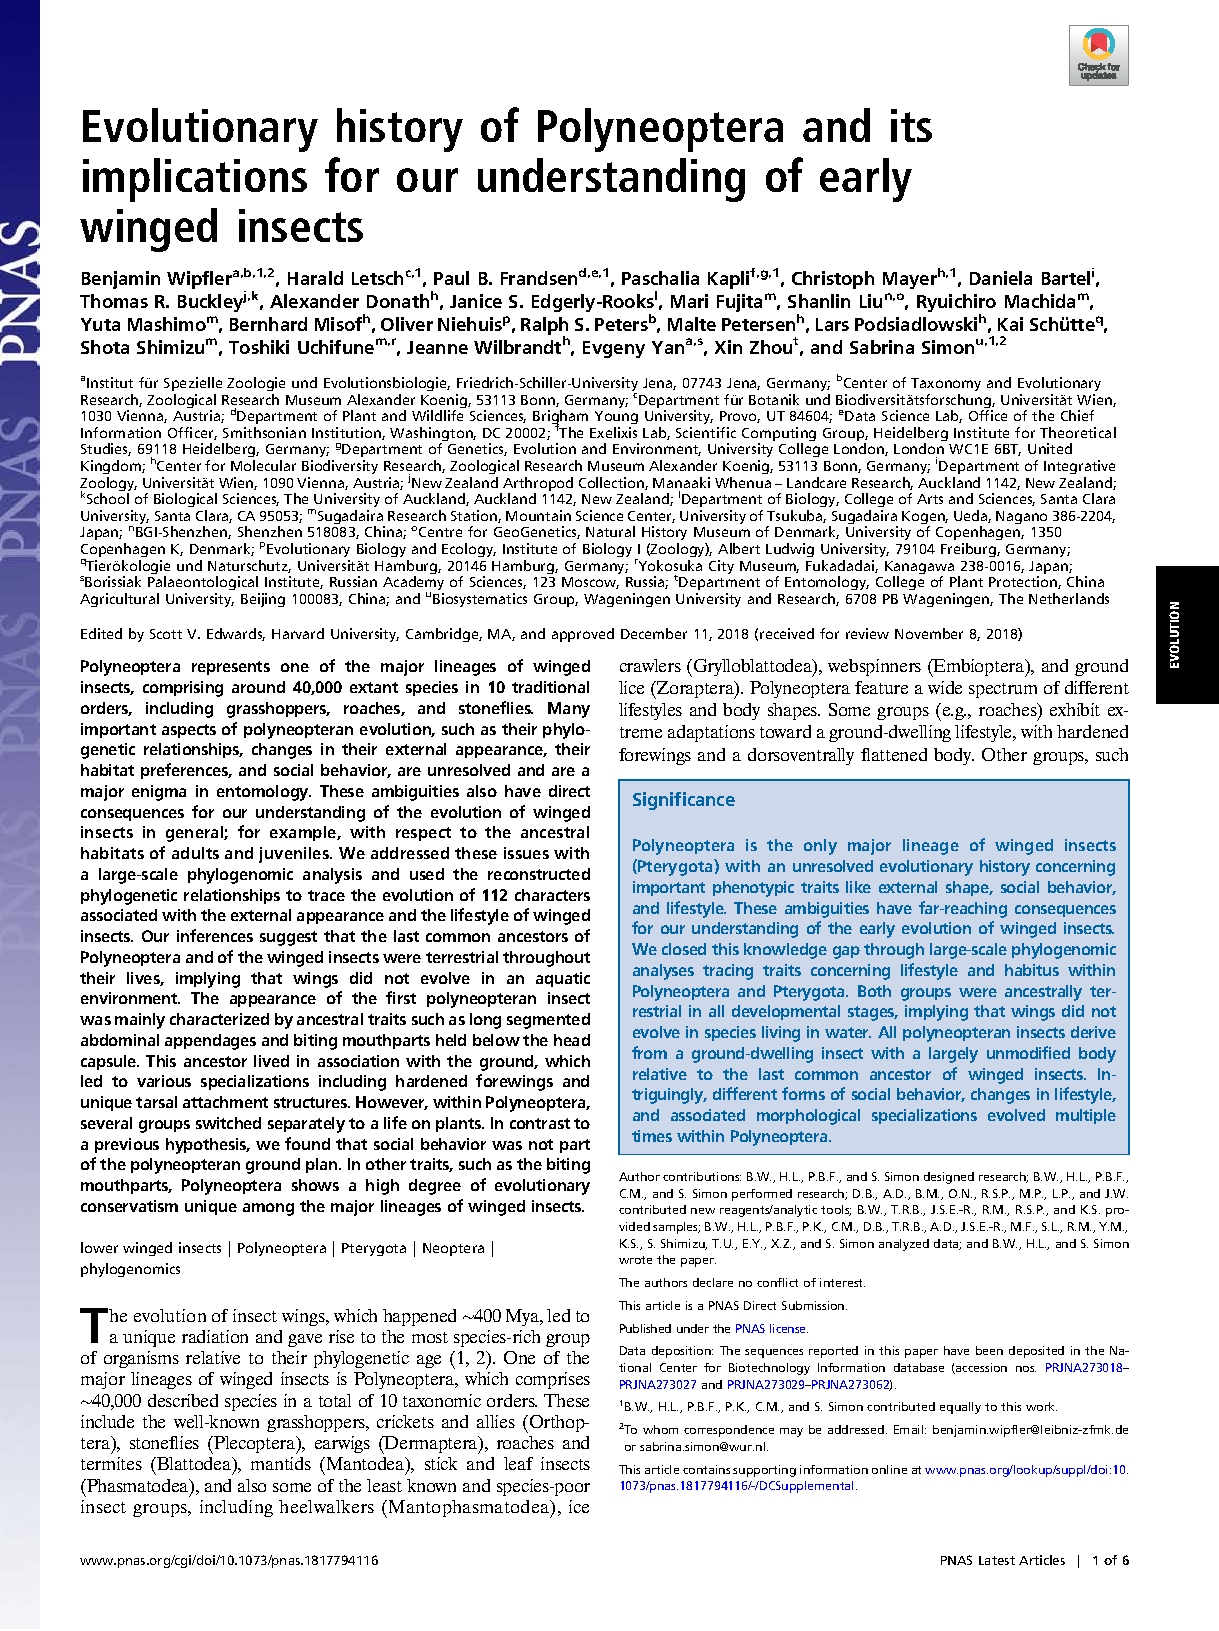
\includepdf[addtotoc={1,section,1,\citet{Wipfler2019}: Evolutionary history of Polyneoptera and its implications for our understanding of early winged insects,app:Wipfler2019},pages=-6]{appendix/A/Wipfler2019} % range without endpoints: from first to last
\includepdf[addtotoc={1,section,1,\citet{Johnson2018}: Phylogenomics and the evolution of hemipteroid insects,app:Johnson2018},pages=-6]{appendix/A/Johnson2018} % range without endpoints: from first to last
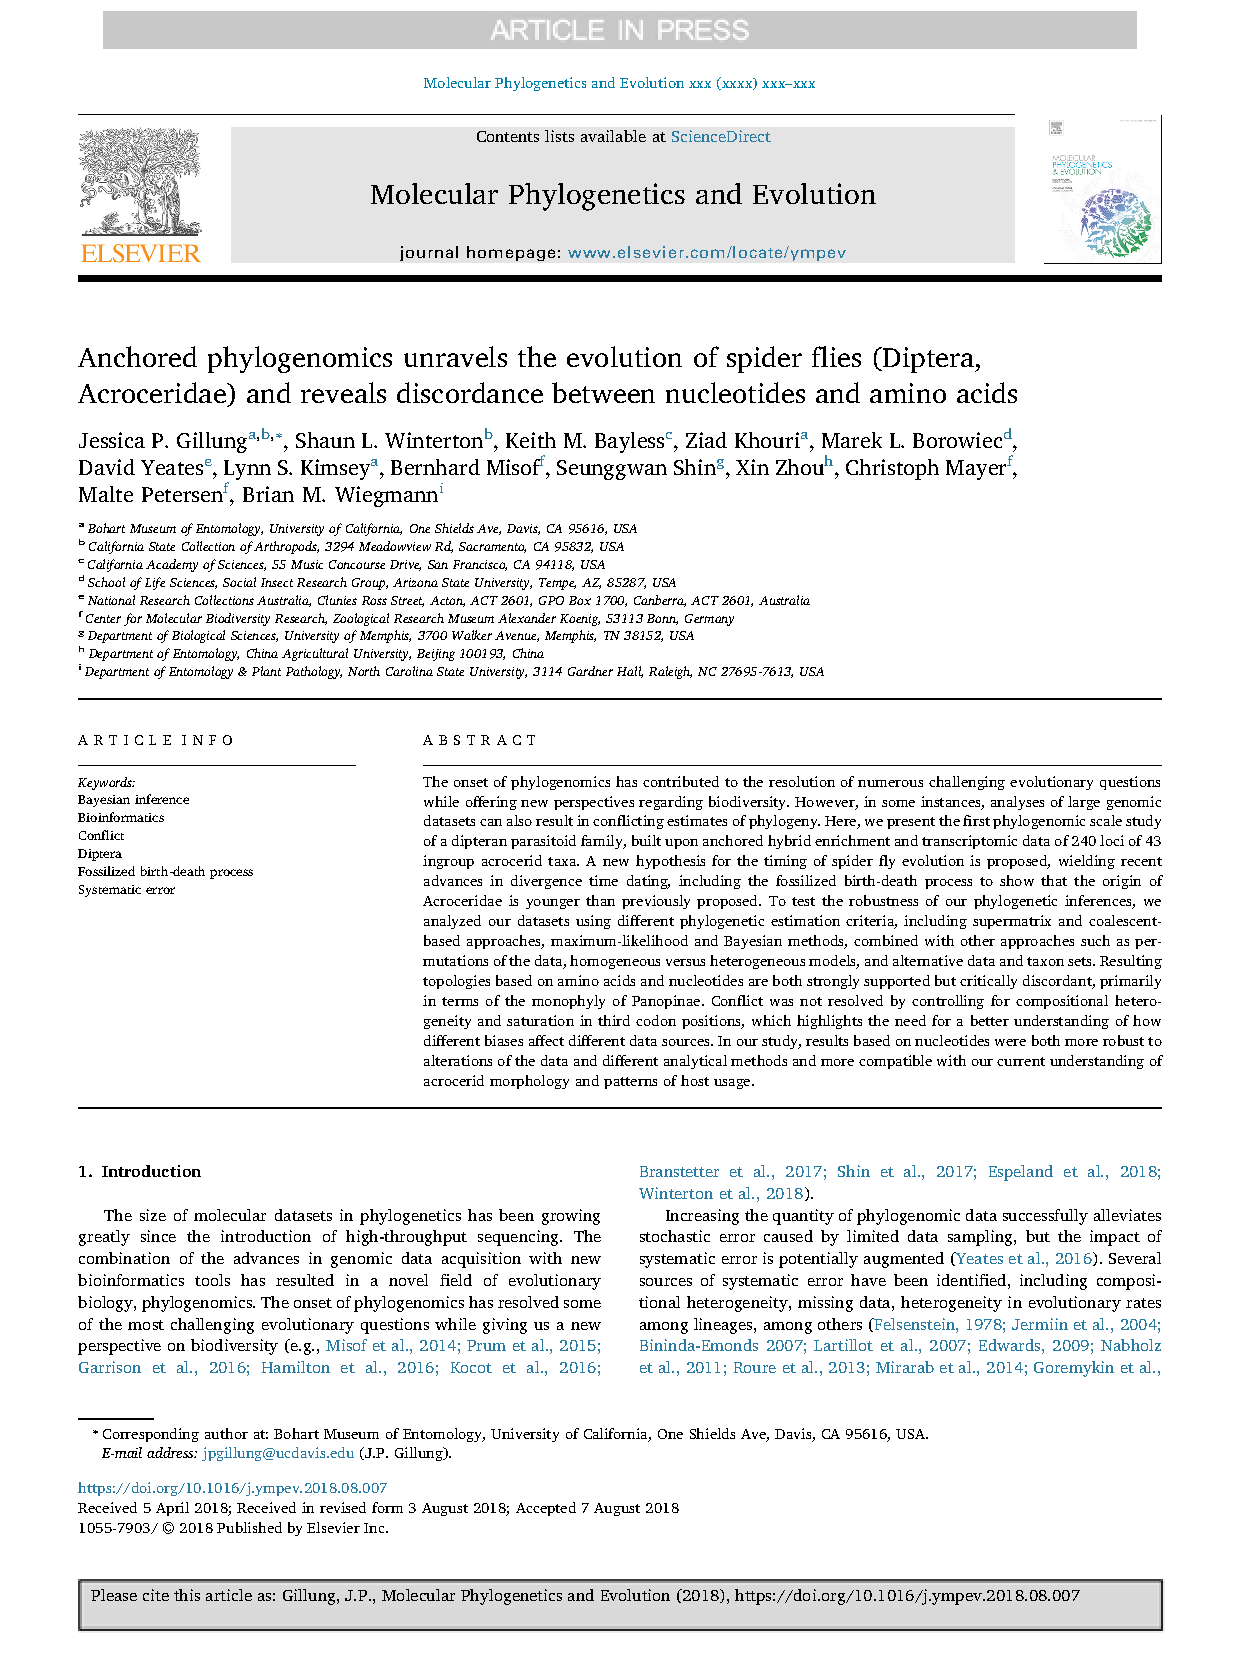
\includepdf[addtotoc={1,section,1,\citet{Gillung2018}: Anchored phylogenomics unravels the evolution of spider flies (Acroceridae) and reveals discordance between nucleotides and amino acids,app:Gillung2018},pages=-]{appendix/A/Gillung2018} % range without endpoints: from first to last
\includepdf[addtotoc={1,section,1,\citet{Peters2017}: Evolutionary history of the Hymenoptera,app:Peters2017},pages=-]{appendix/A/Peters2017} % range without endpoints: from first to last
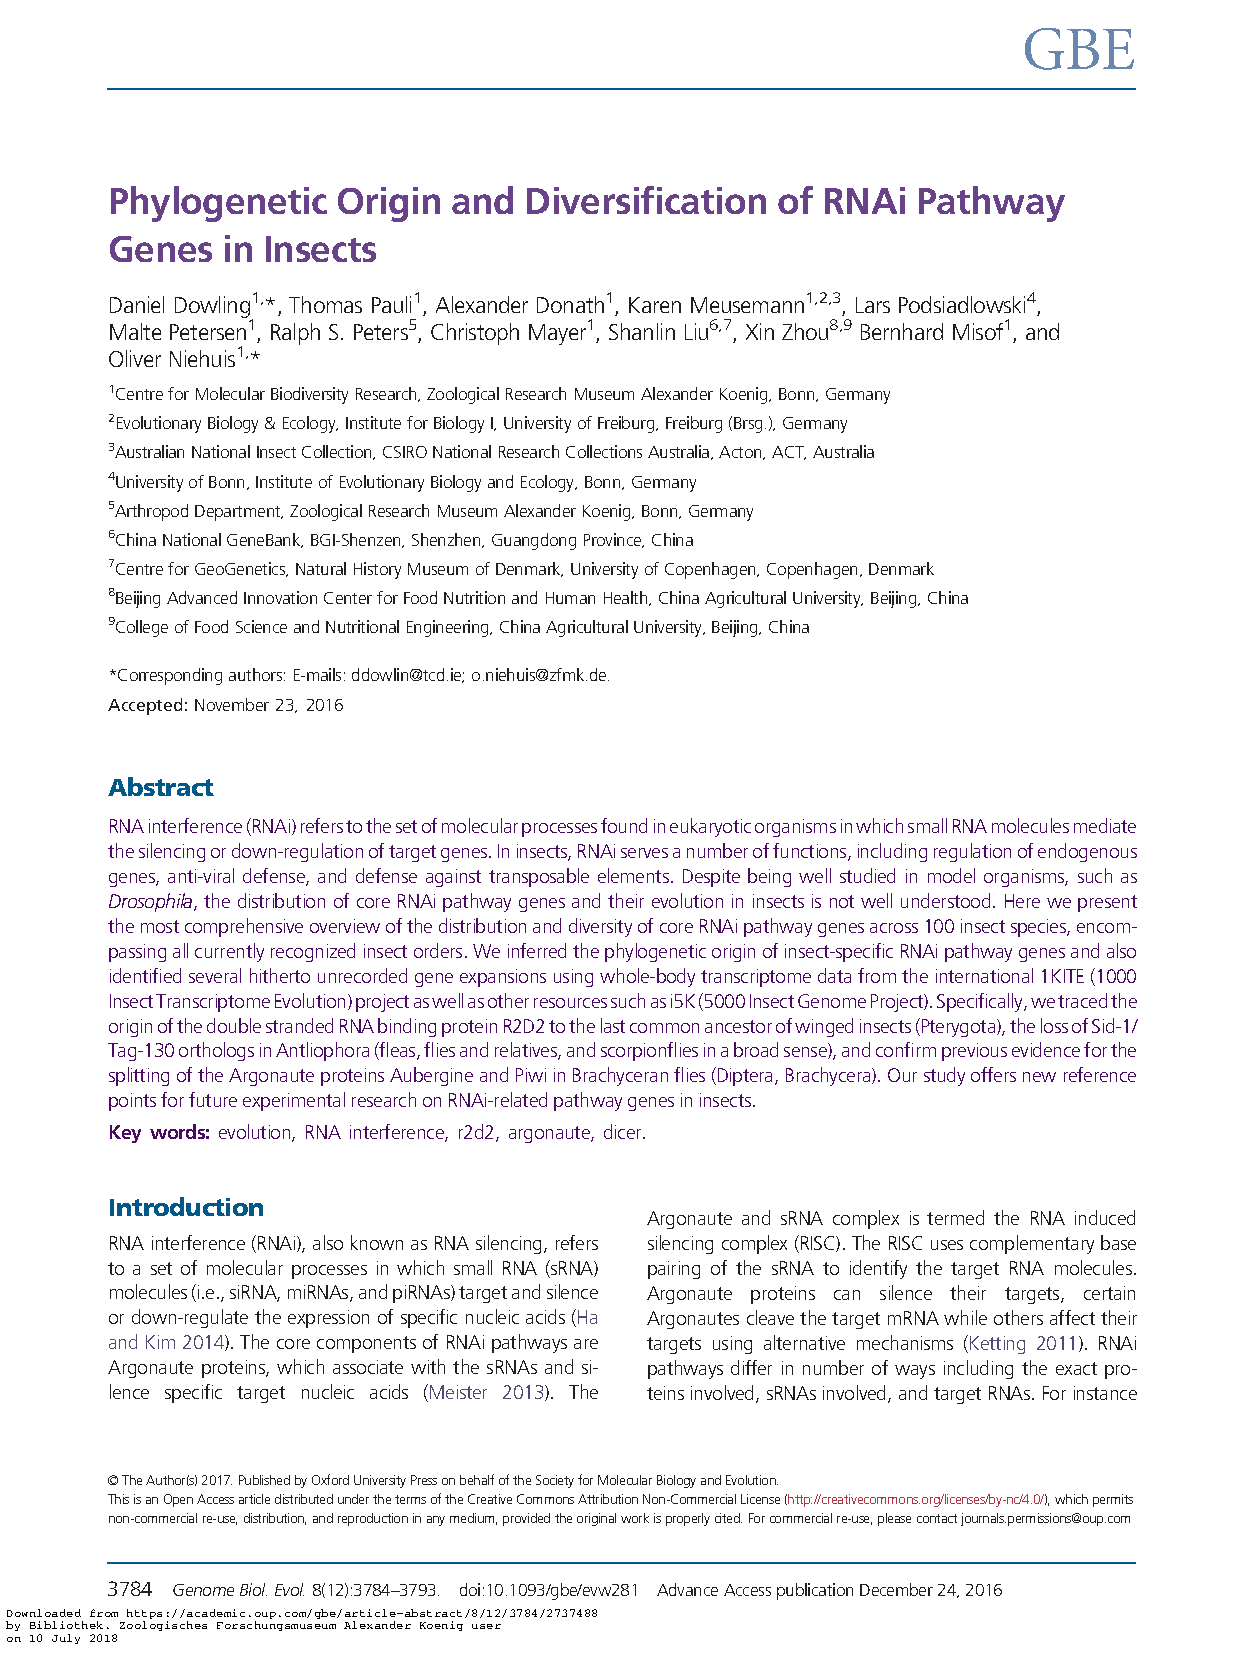
\includepdf[addtotoc={1,section,1,\citet{Dowling2017}: Phylogenetic origin and diversification of RNAi pathway genes in insects,app:Dowling2017},pages=-]{appendix/A/Dowling2017}
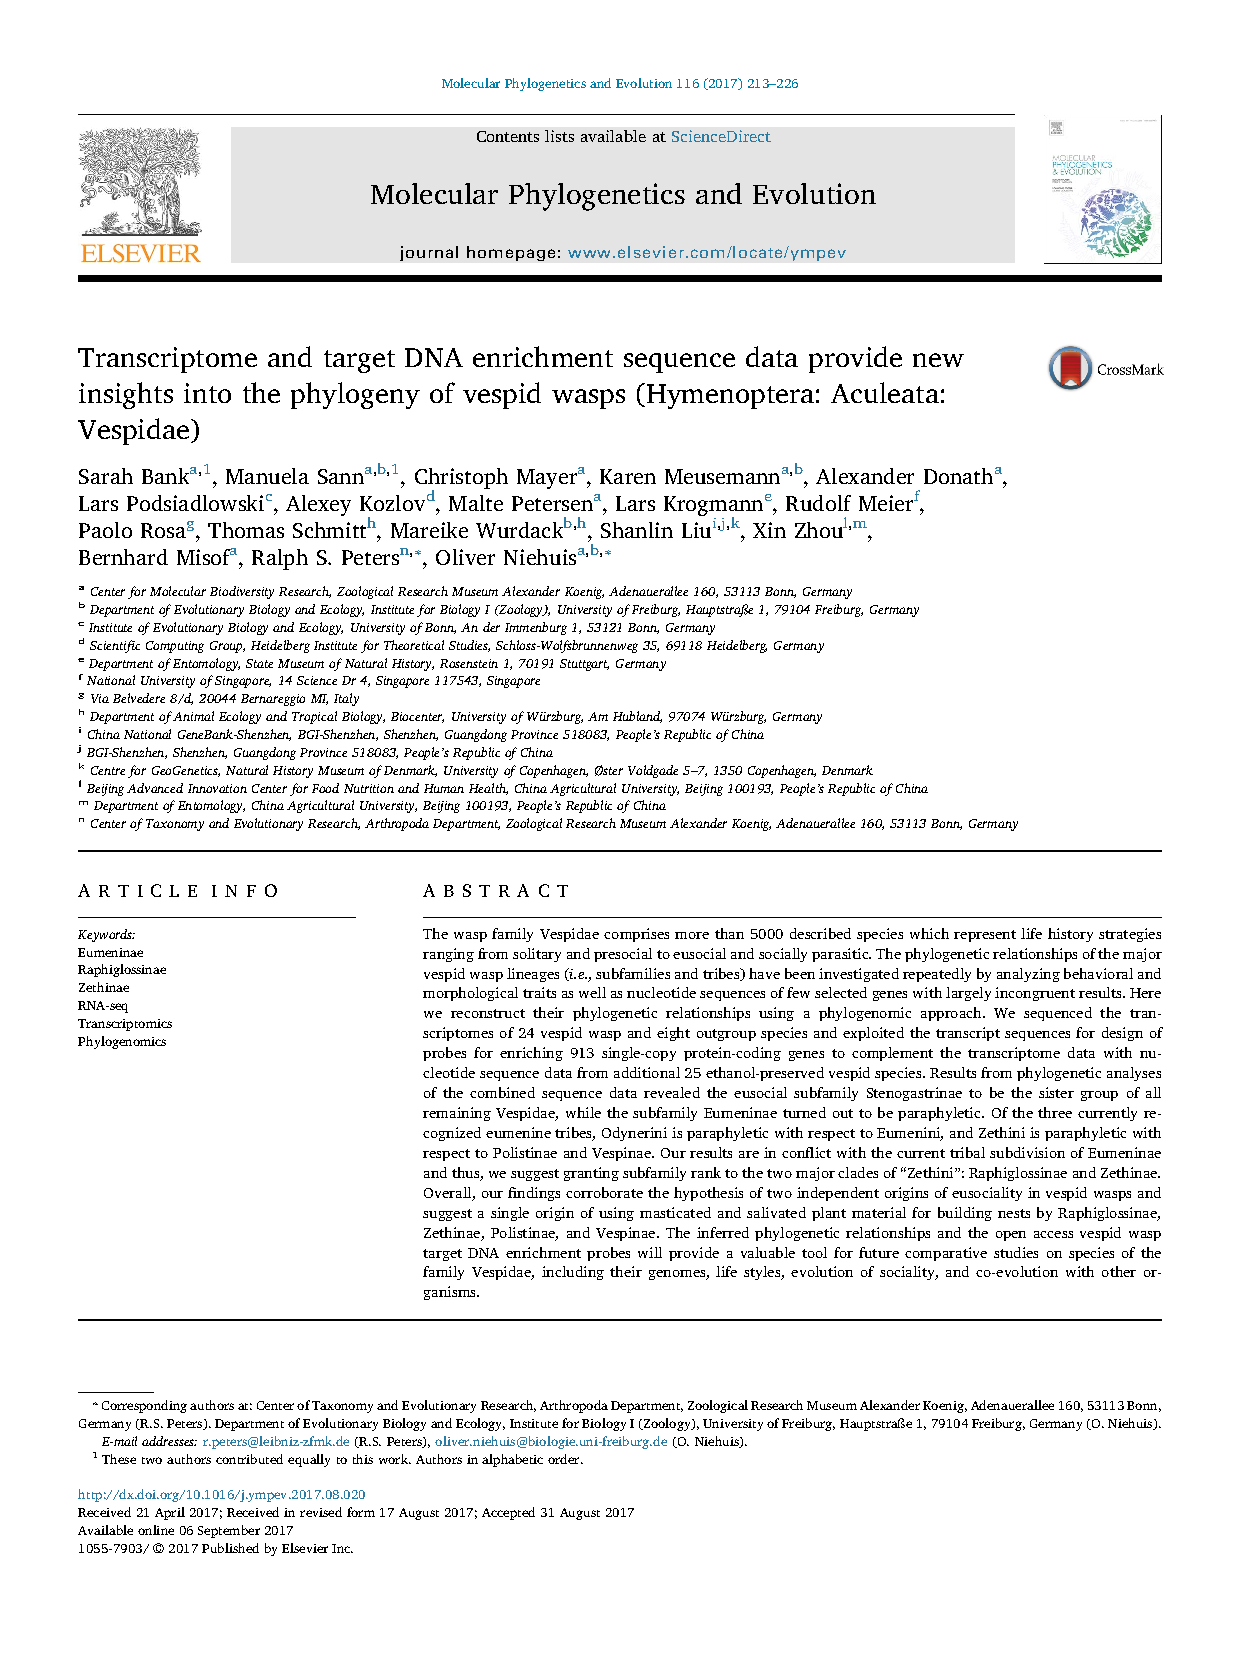
\includepdf[addtotoc={1,section,1,\citet{Bank2017}: New insights into the phylogeny of vespid wasps (Hymenoptera: Aculeata: Vespidae),app:Bank2017},pages=-]{appendix/A/Bank2017}
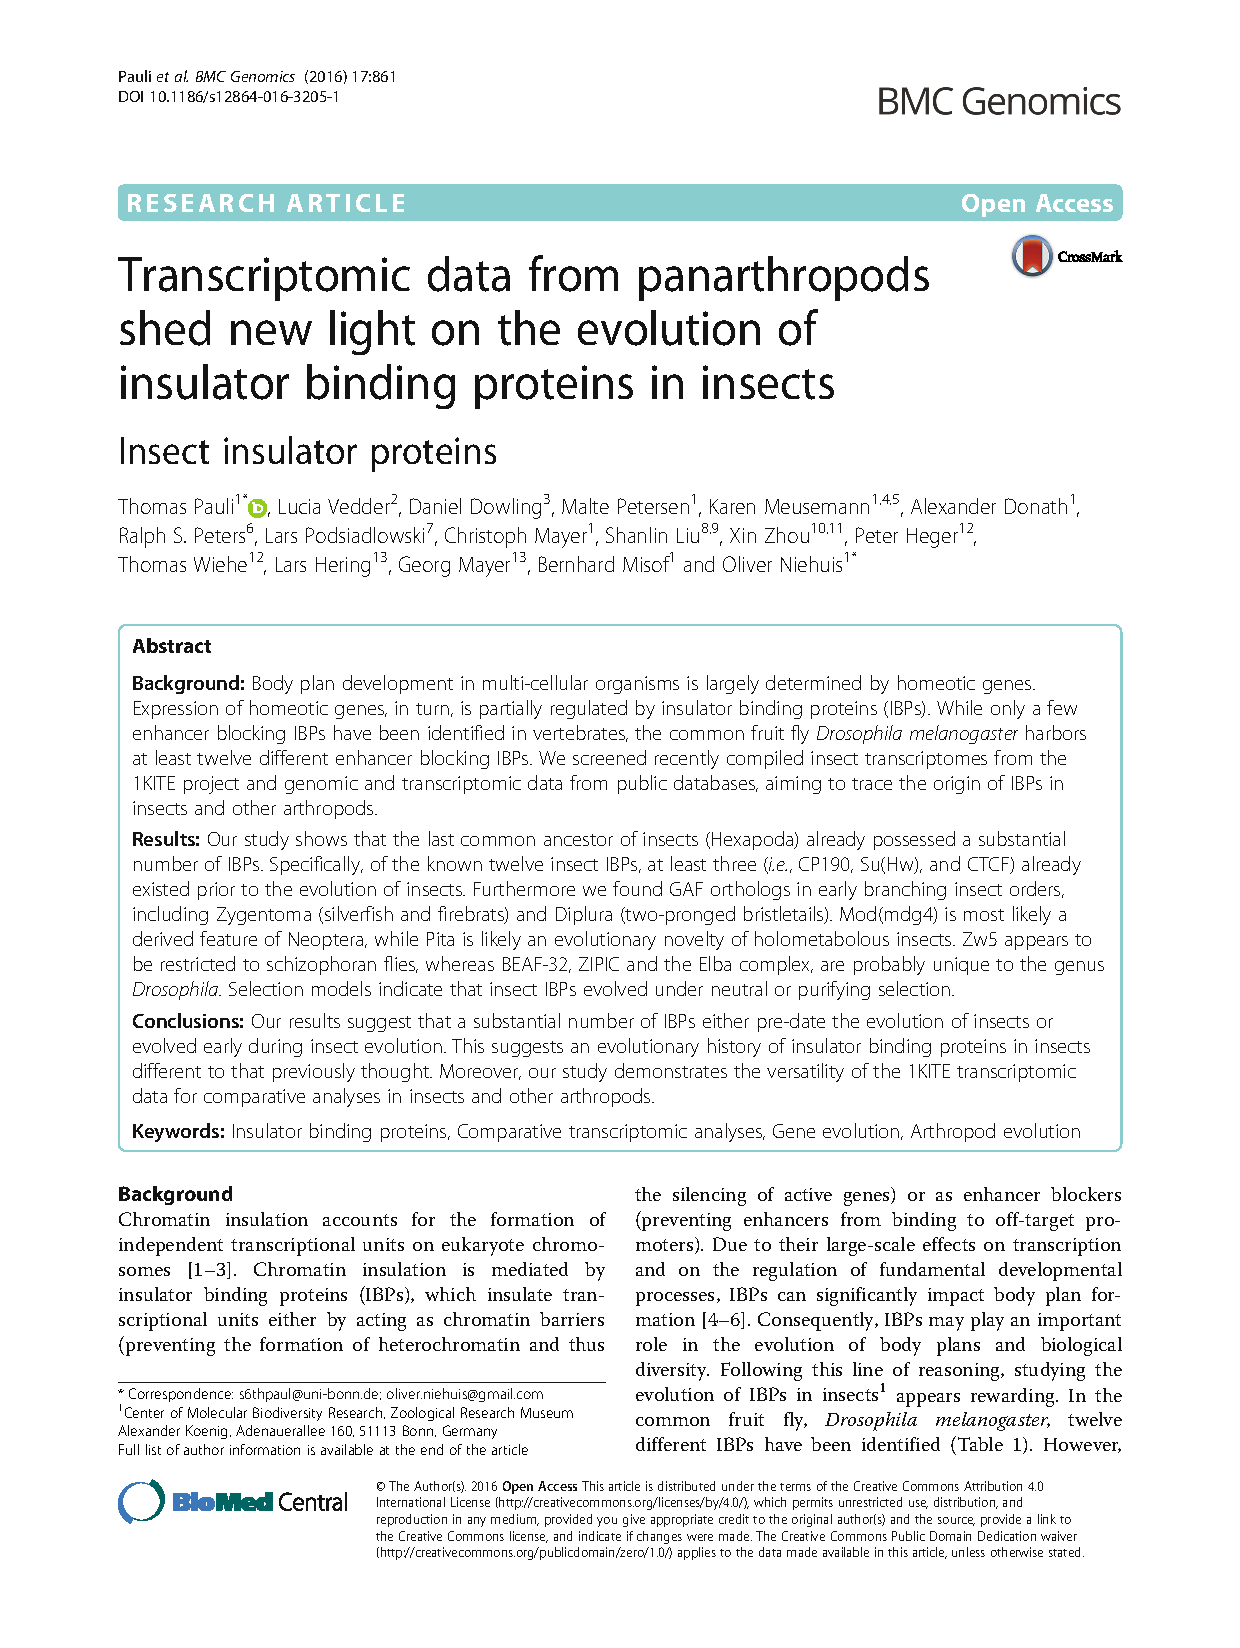
\includepdf[addtotoc={1,section,1,\citet{Pauli2016}: New insights on the evolution of insulator binding proteins in insects,app:Pauli2016},pages=-]{appendix/A/Pauli2016}
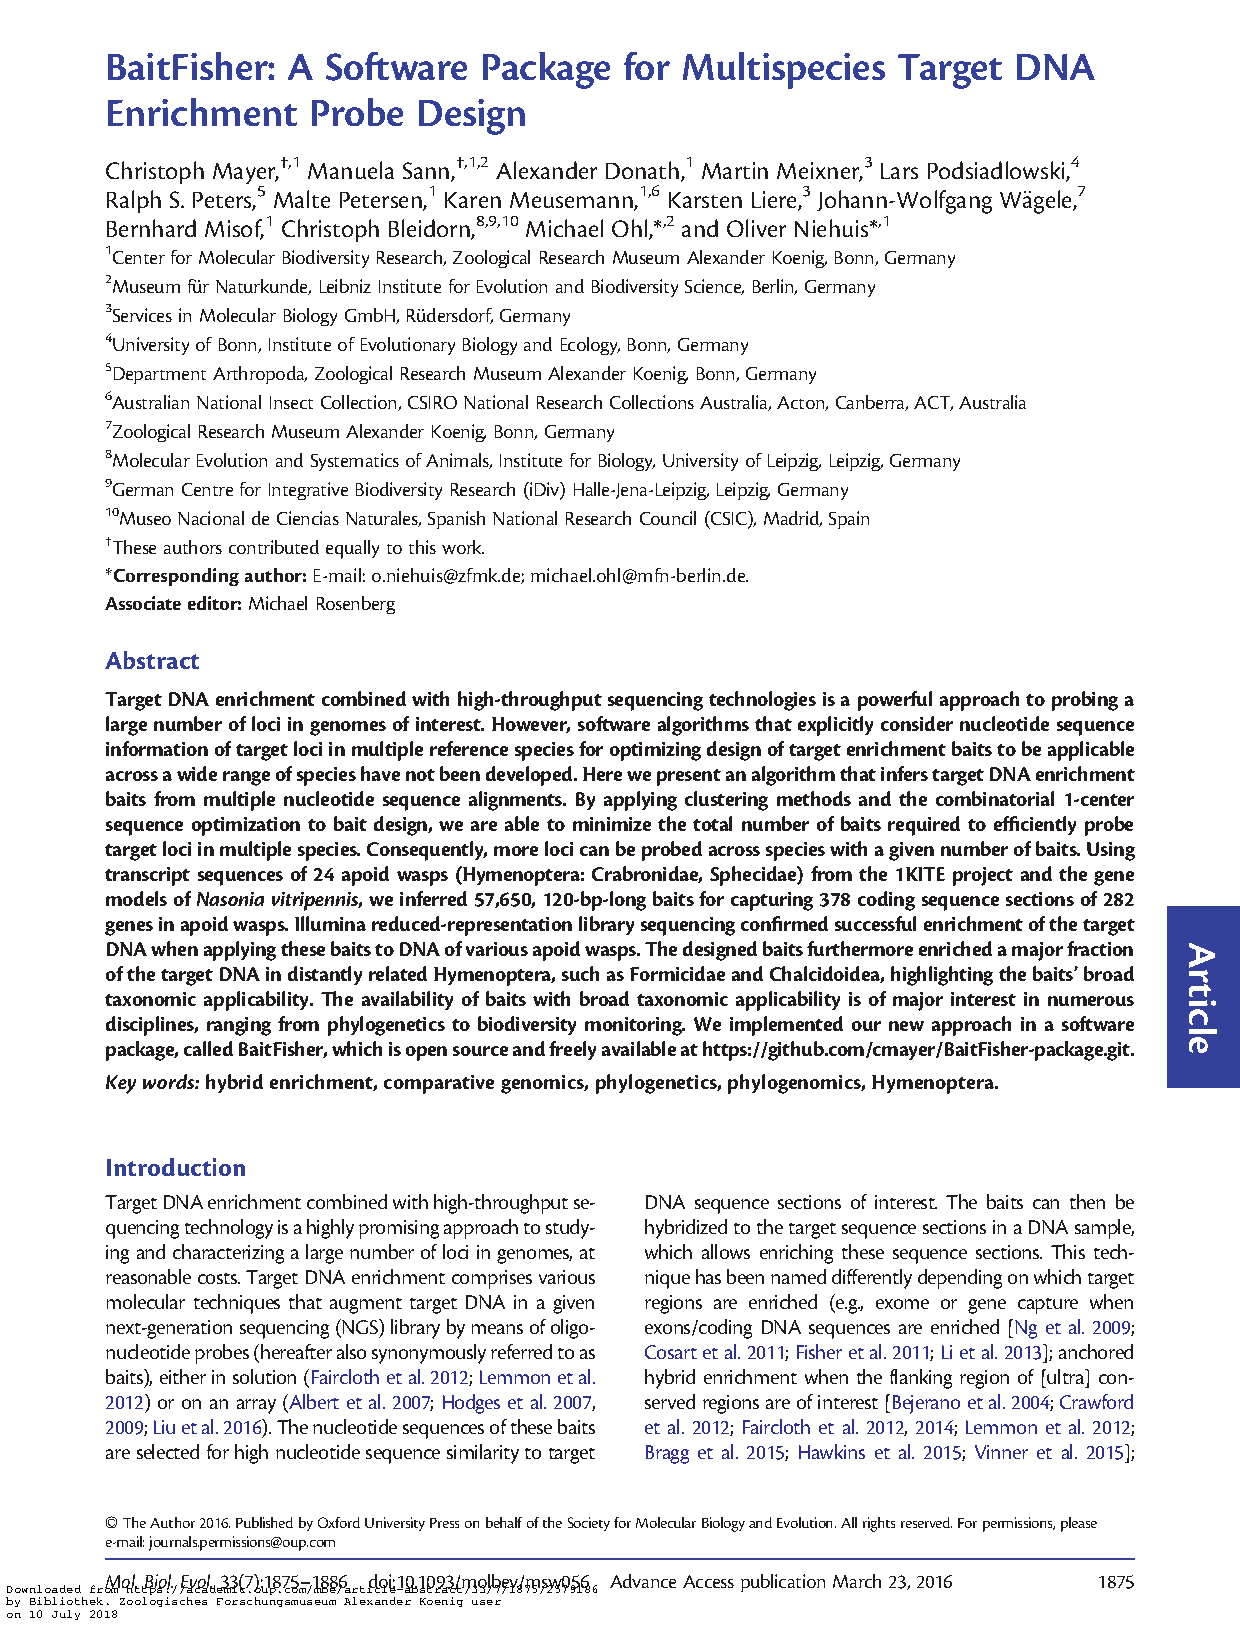
\includepdf[addtotoc={1,section,1,\citet{Mayer2016}: BaitFisher: A software package for multispecies target DNA enrichment probe design,app:Mayer2016},pages=-]{appendix/A/Mayer2016}
}

	%!TEX root = ../dissertation.tex
\chapter{Other co-authored publications}
\label{app:other-publications}

\ifdraft{%
	\section{\citet{Astrin2016}}
	\emptypages{24} % Astrin 2016
	\section{\citet{Kraaijeveld2016}}
	\emptypages{11} % Kraaijeveld2016
	\section{\citet{Struck2014}}
	\emptypages{17} % Struck2014
	\section{\citet{Peters2014}}
	\emptypages{16} % Peters2014
	\section{\citet{Misof2014}\label{app:Misof2014}}
	\emptypages{5} % Misof2014
	\section{\citet{Dell'Ampio2014}}
	\emptypages{11} % Dell'Ampio 2014
	\section{\citet{Niehuis2012}}
	\emptypages{5} % Niehuis2012
}%
{%
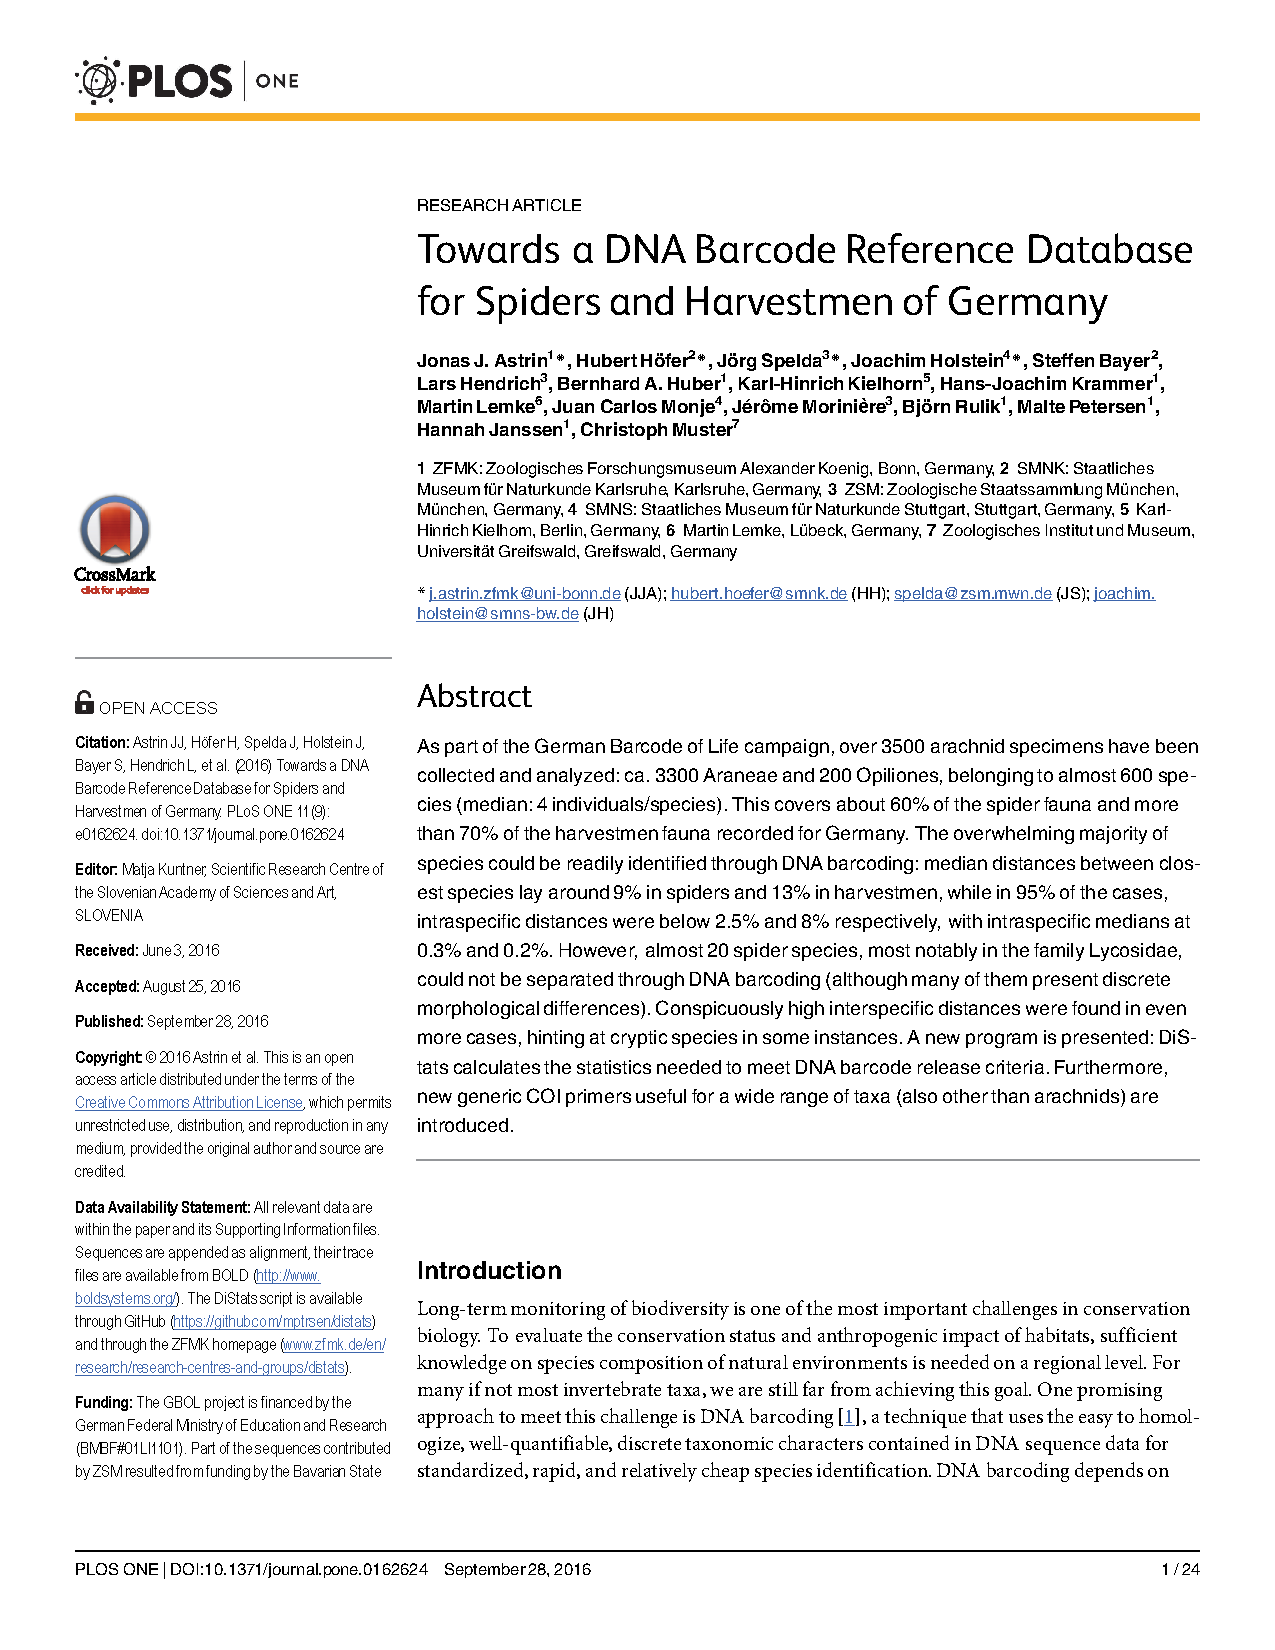
\includepdf[addtotoc={1,section,1,\citet{Astrin2016}: Towards a DNA barcode reference database for spiders and harvestmen of germany,app:Astrin2016},pages=-]{appendix/B/Astrin2016} % range without endpoints: from first to last
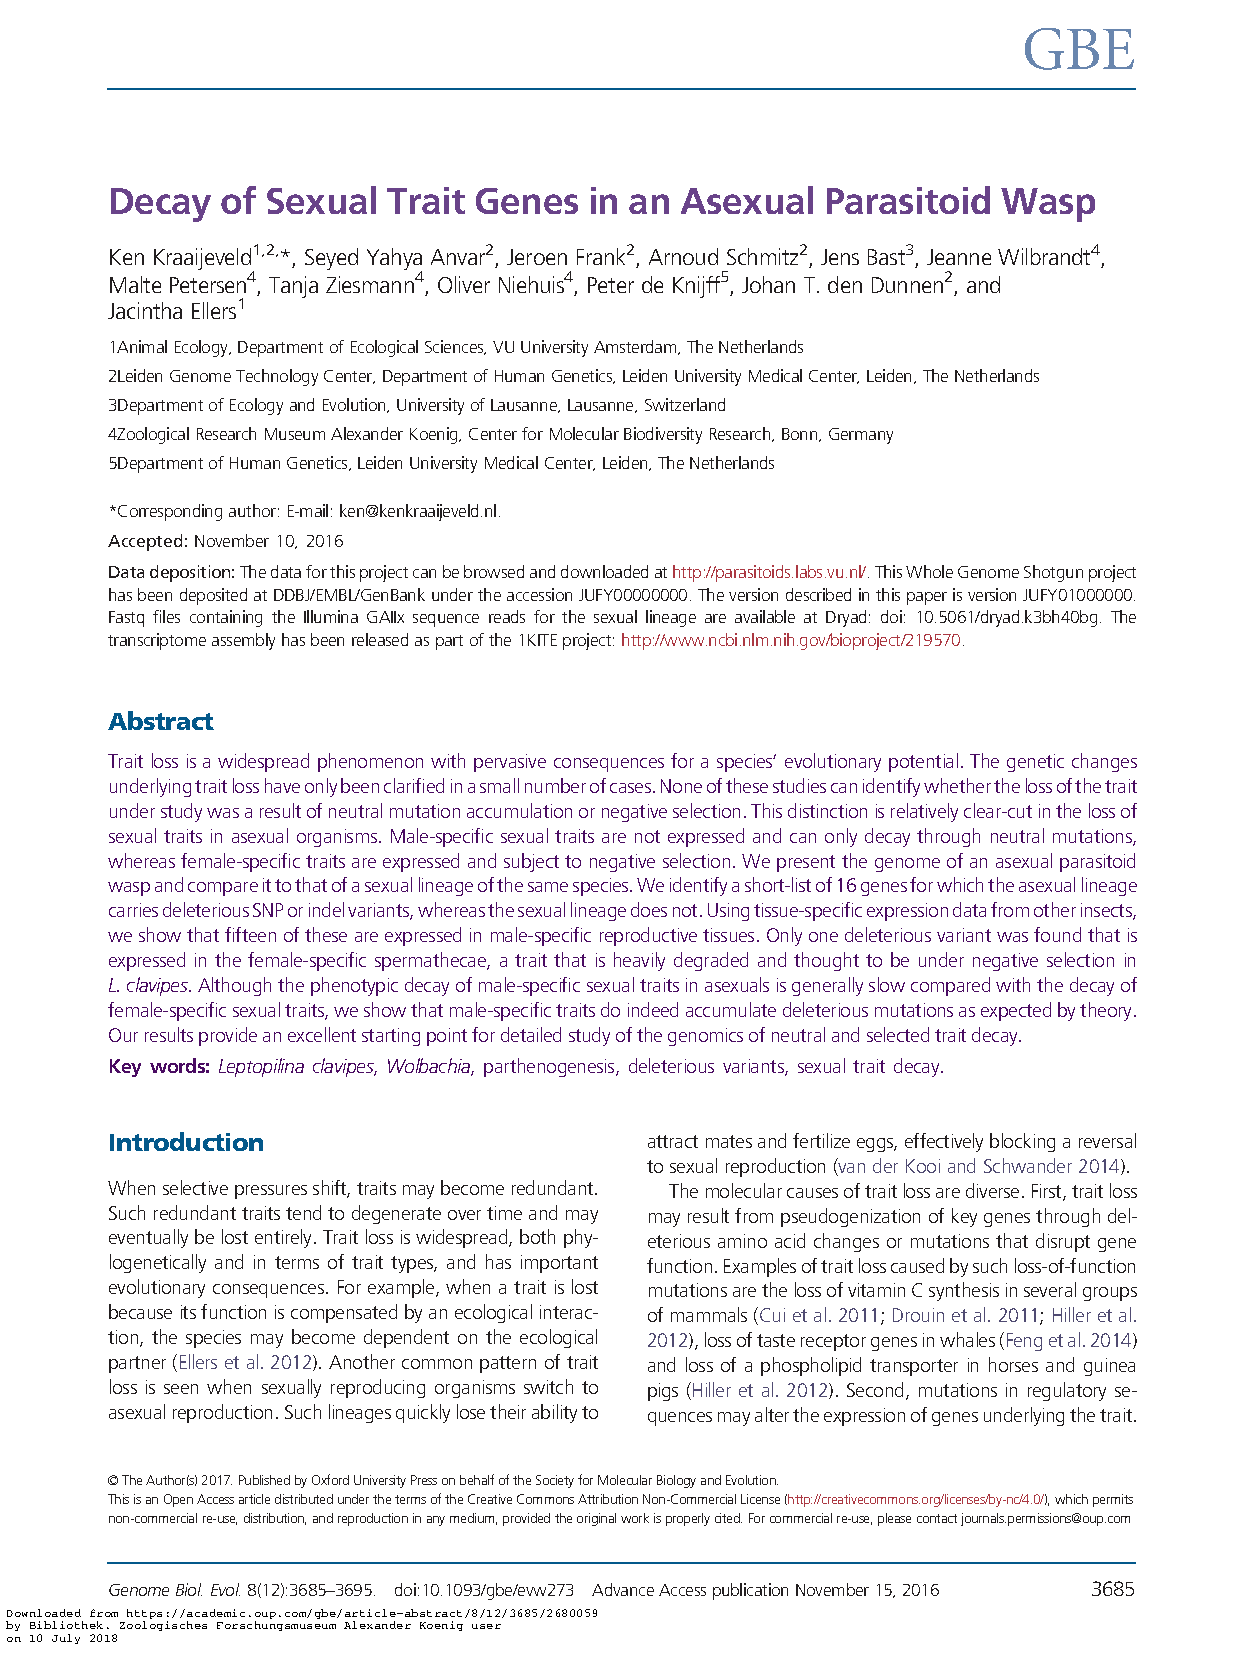
\includepdf[addtotoc={1,section,1,\citet{Kraaijeveld2016}: Decay of sexual trait genes in an asexual parasitoid wasp,app:Kraaijeveld2016},pages=-]{appendix/B/Kraaijeveld2016} % range without endpoints: from first to last
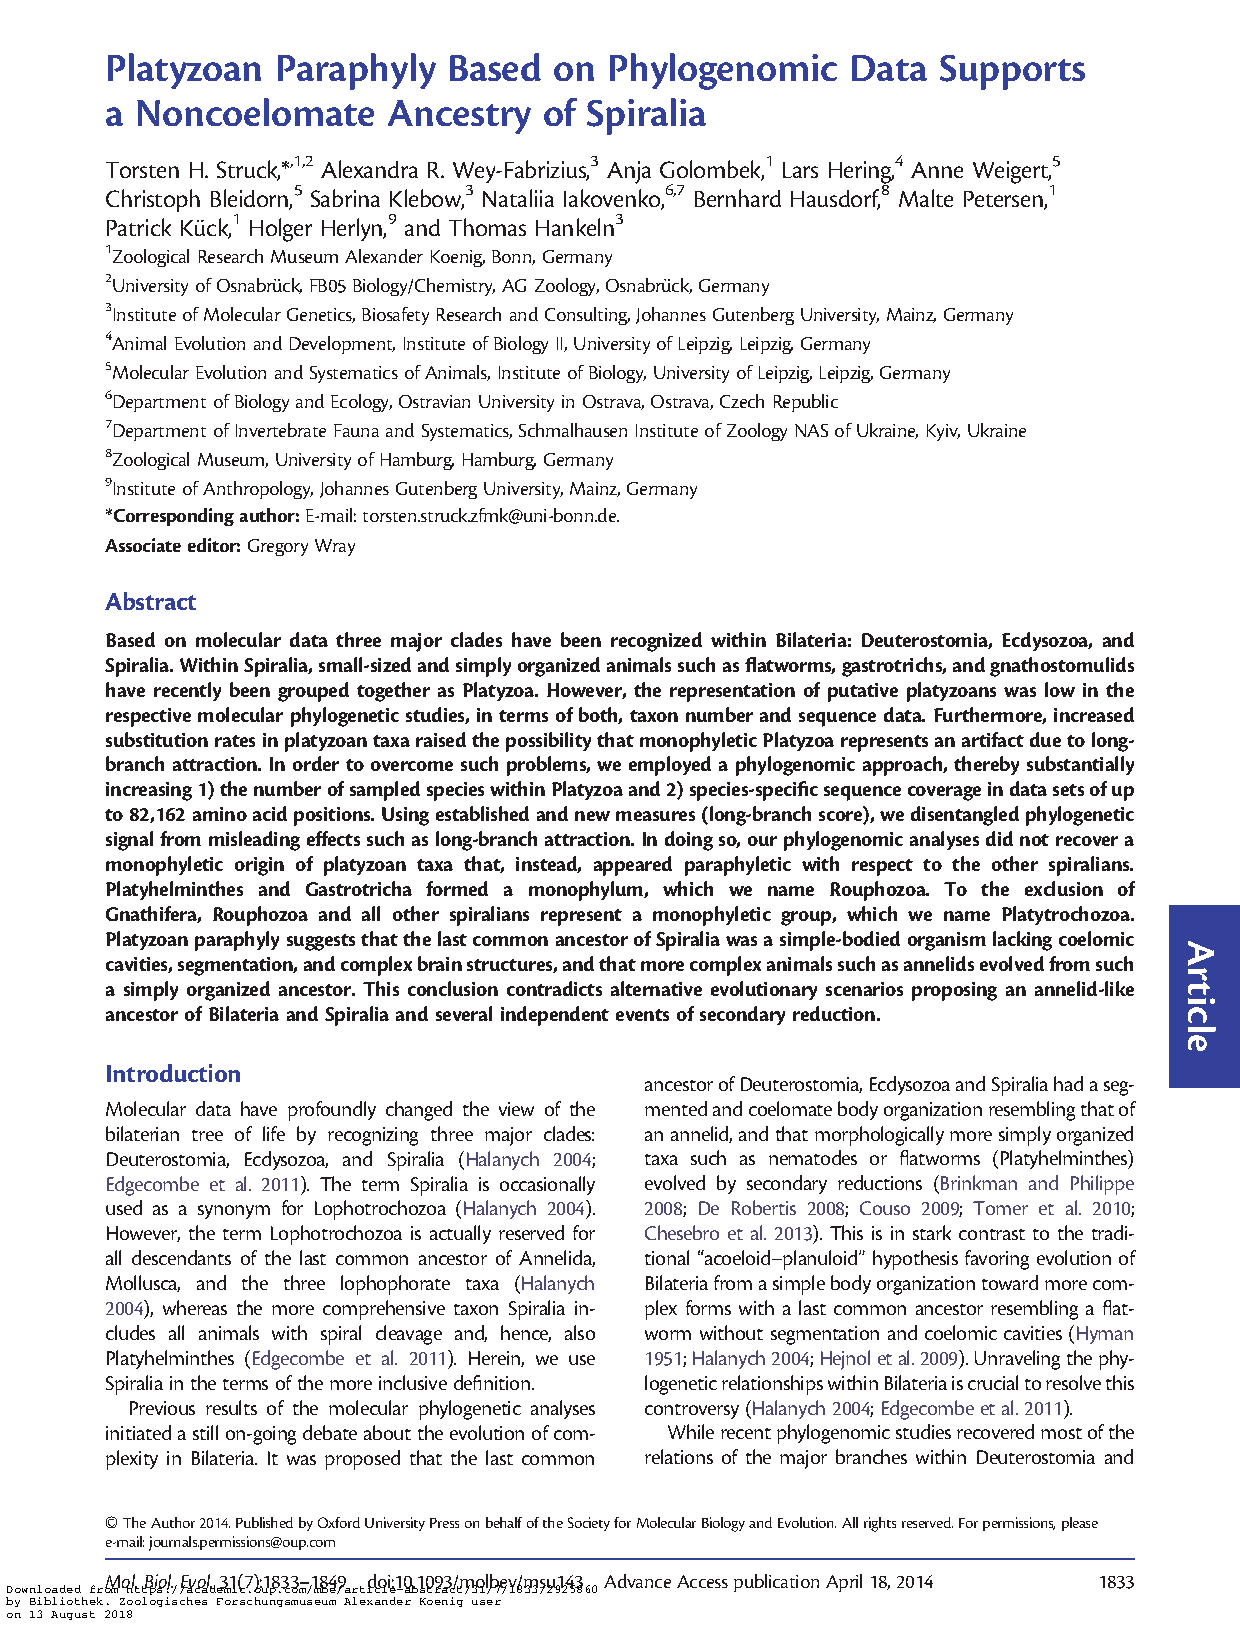
\includepdf[addtotoc={1,section,1,\citet{Struck2014}: Platyzoan paraphyly based on phylogenomic data supports a noncoelomate ancestry of Spiralia,app:Struck2014},pages=-]{appendix/B/Struck2014} % range without endpoints: from first to last
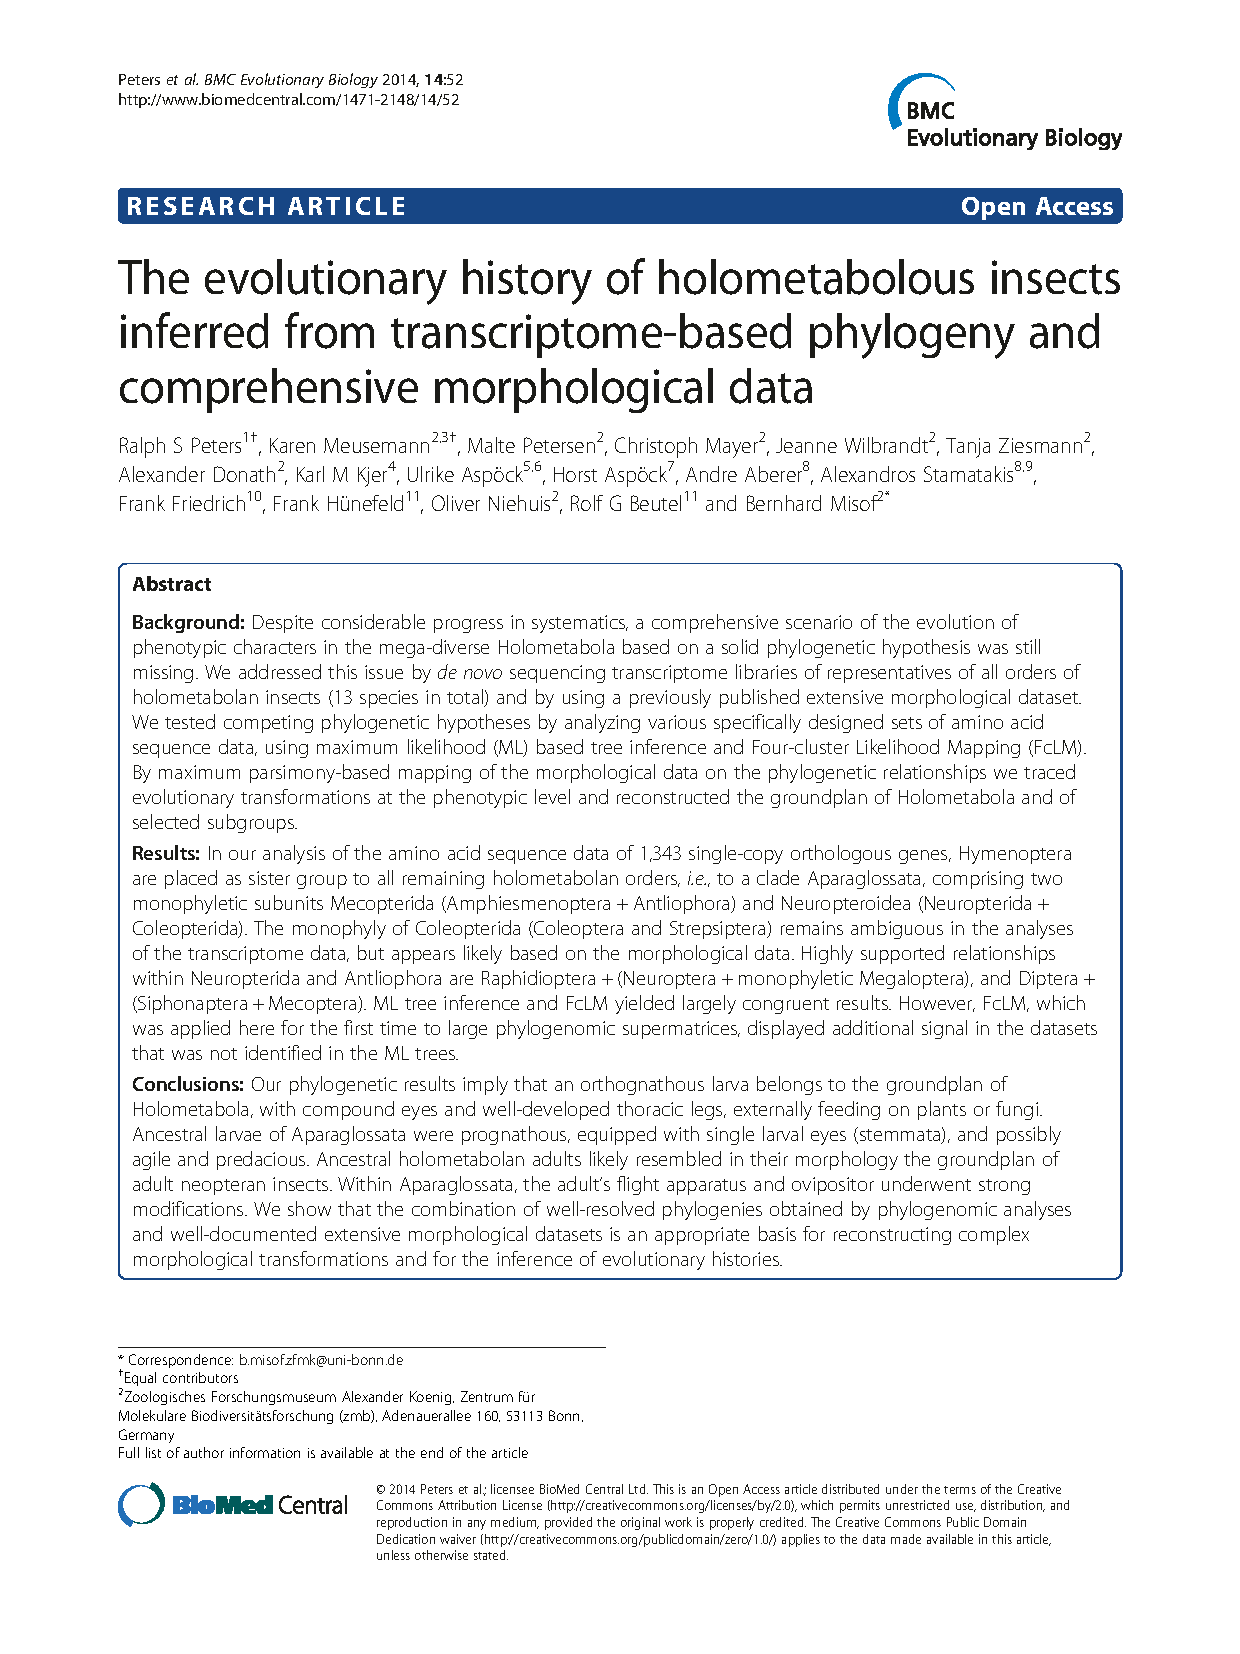
\includepdf[addtotoc={1,section,1,\citet{Peters2014}: The evolutionary history of holometabolous insects inferred from transcriptome-based phylogeny and comprehensive morphological data,app:Peters2014},pages=-]{appendix/B/Peters2014} % range without endpoints: from first to last
\label{app:Misof2014}
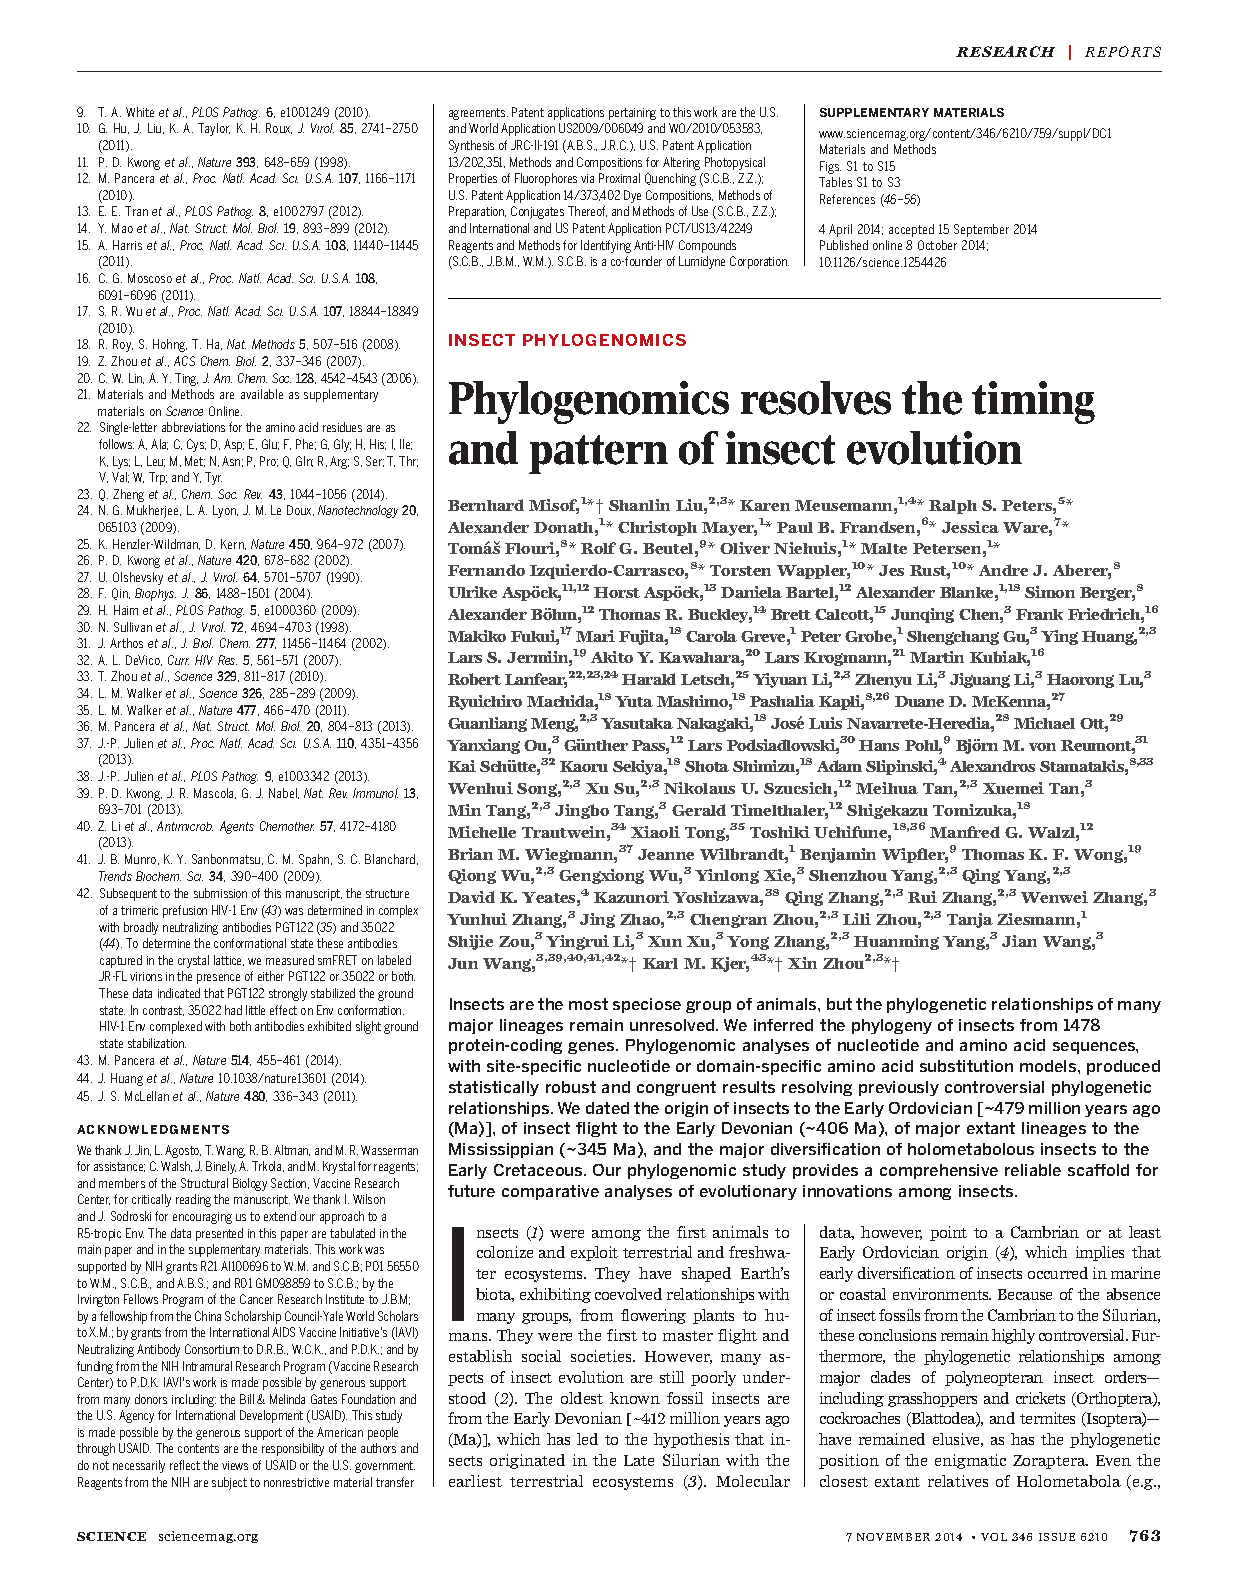
\includepdf[addtotoc={1,section,1,\citet{Misof2014}: Phylogenomics resolves the timing and pattern of insect evolution,app:Misof2014},pages=-]{appendix/B/Misof2014} % range without endpoints: from first to last
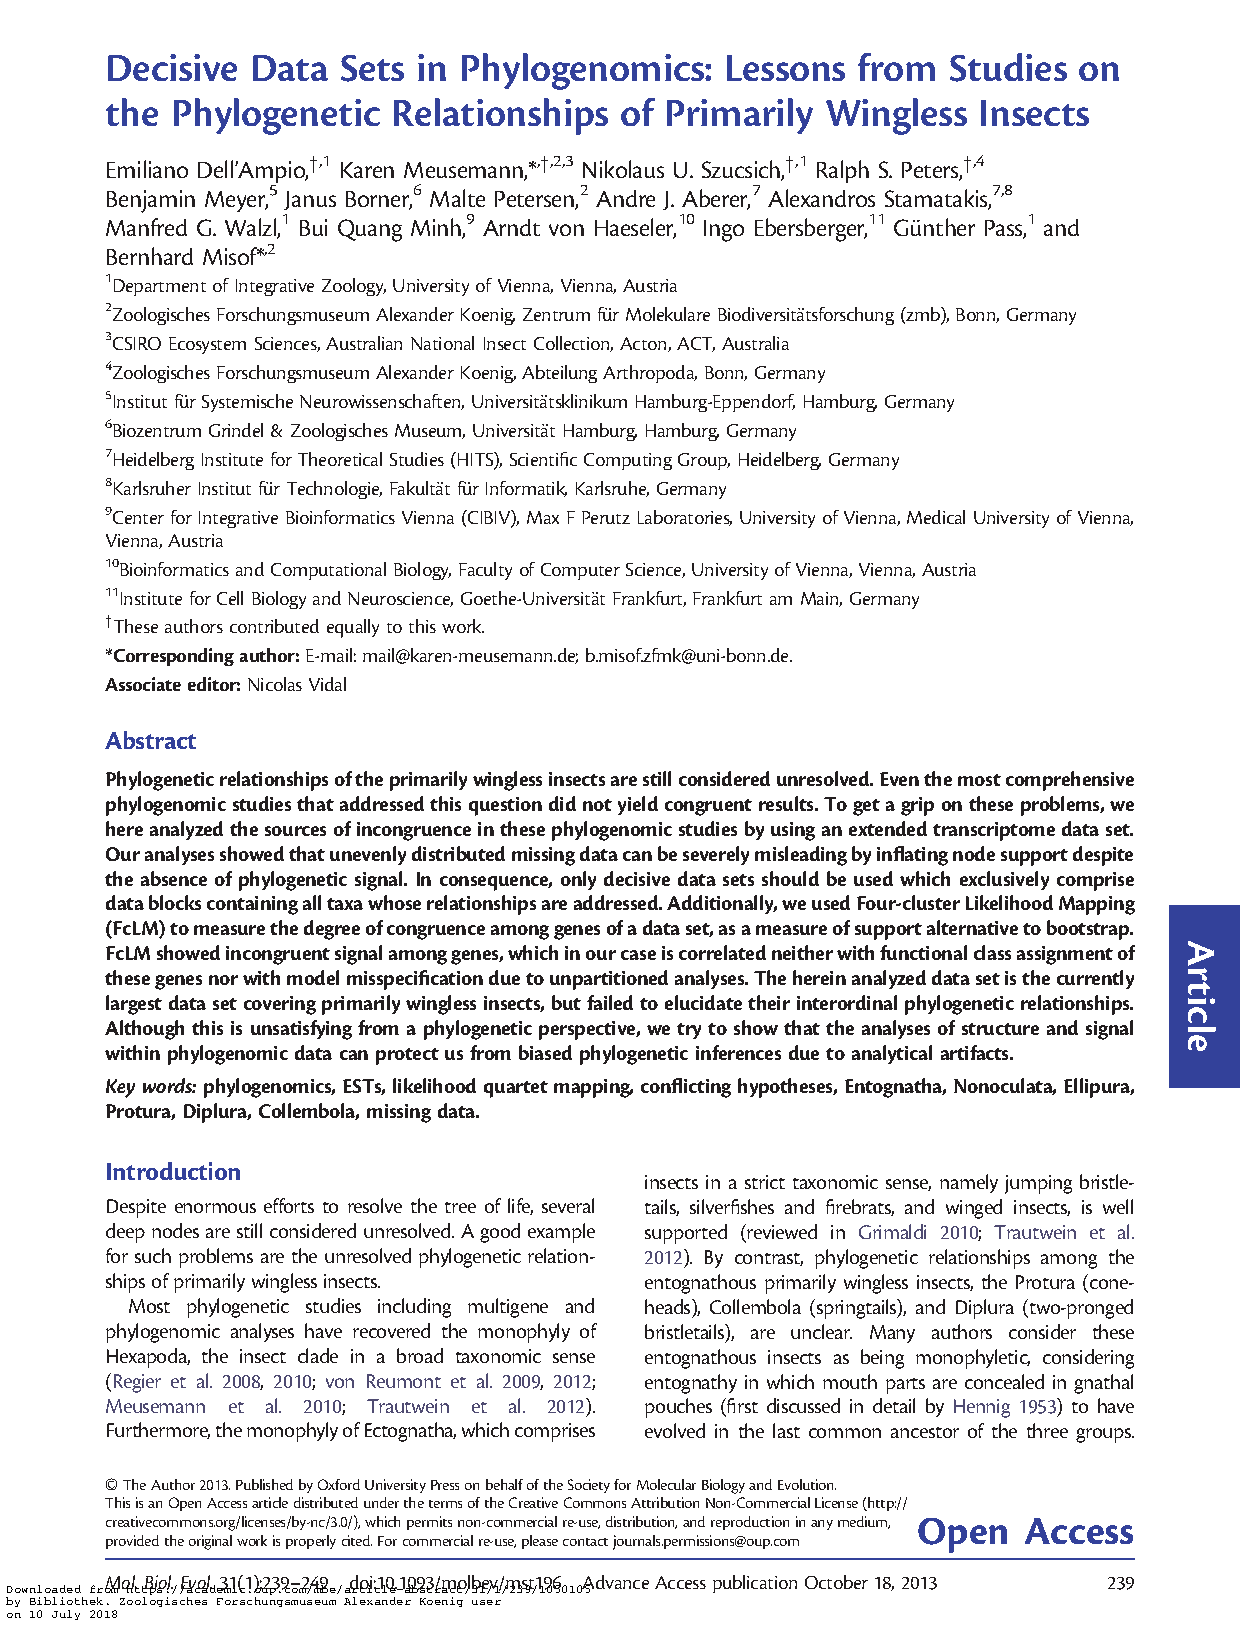
\includepdf[addtotoc={1,section,1,\citet{Dell'Ampio2014}: Decisive data sets in phylogenomics: lessons from studies on the phylogenetic relationships of primarily wingless insects,app:Dell'Ampio2014},pages=-]{appendix/B/DellAmpio2014} % range without endpoints: from first to last
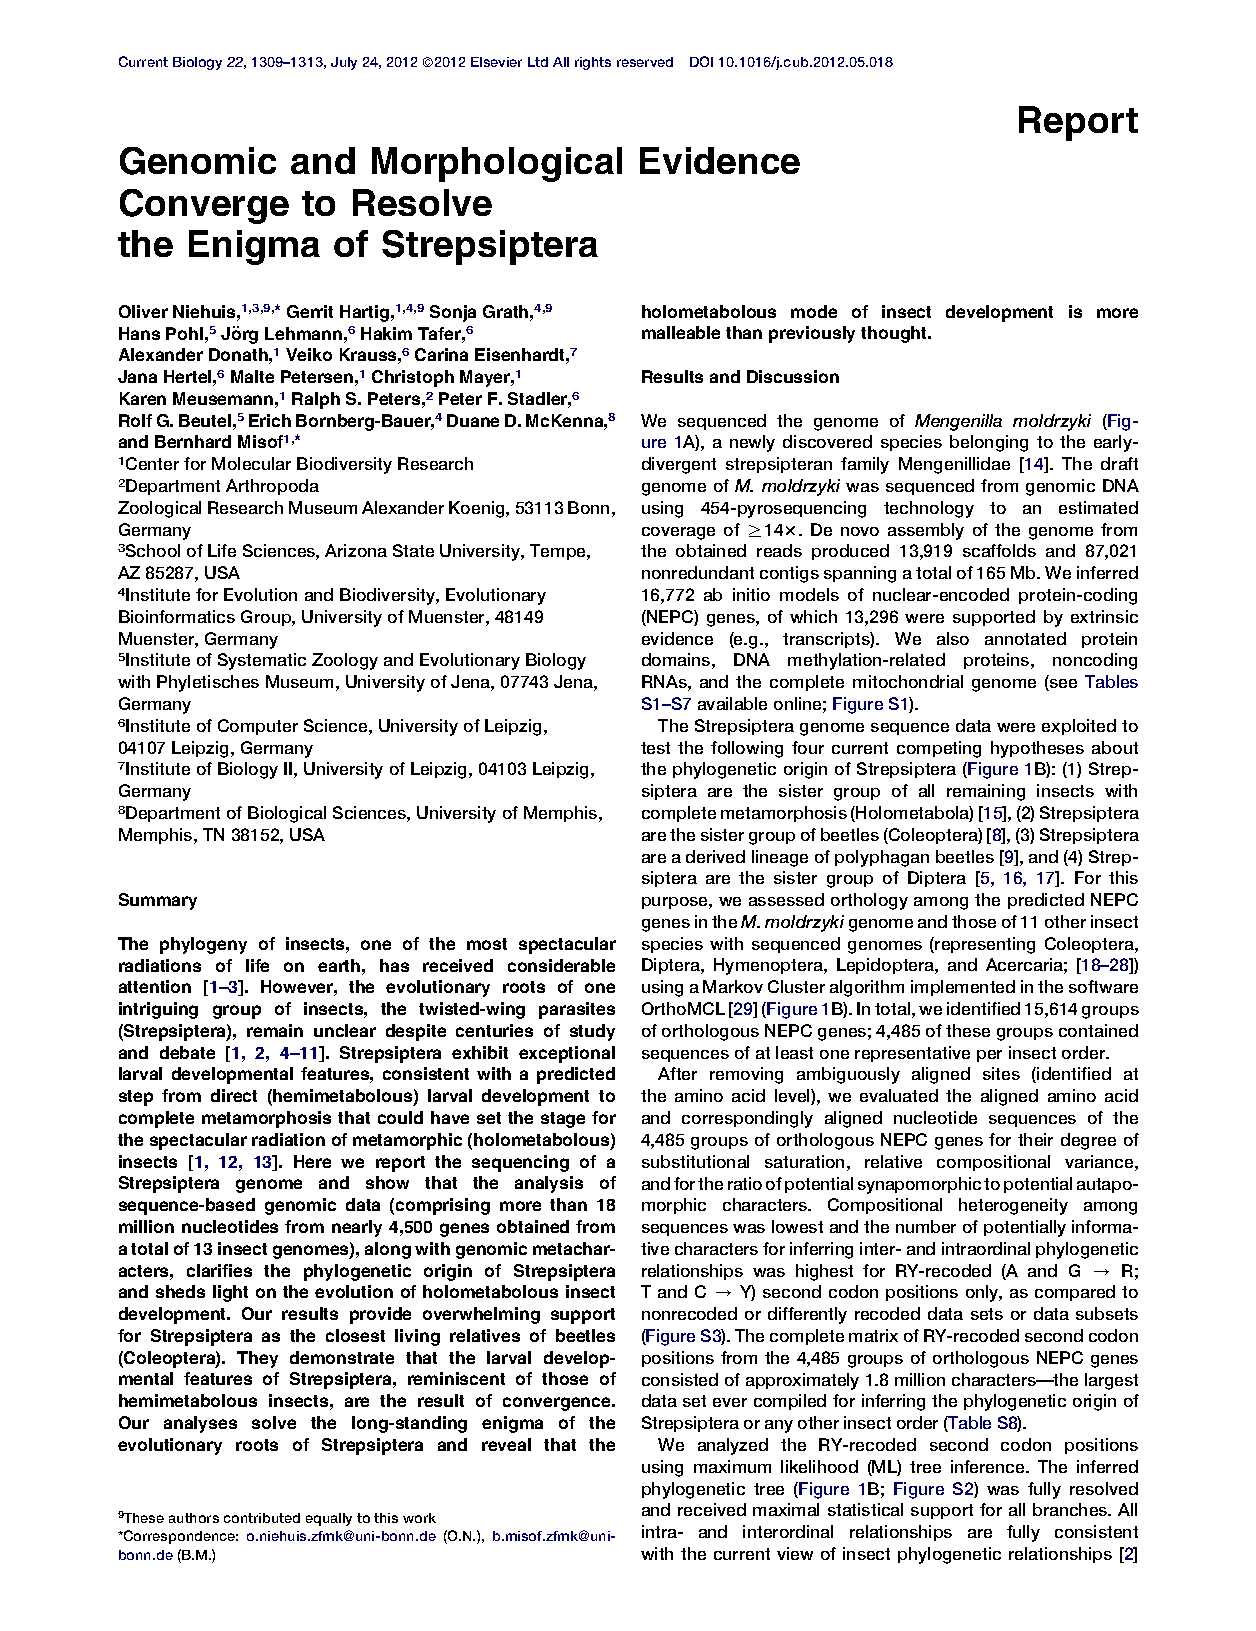
\includepdf[addtotoc={1,section,1,\citet{Niehuis2012}: Genomic and morphological evidence converge to resolve the enigma of Strepsiptera,app:Niehuis2012},pages=-]{appendix/B/Niehuis2012} % range without endpoints: from first to last
}%

	\chapter{Supplemental material to chapter \ref{cha:mobilome}}

Supplemental methods, figures, and data tables:

\begin{itemize}
	\item Figure \ref{fig:te-families-vs-genome-size}: The number of TE superfamilies is significantly correlated to genome size (page \pageref{fig:te-families-vs-genome-size})
\end{itemize}

\begin{itemize}
	\item Table \ref{tab:patterns}: Word patterns to exclude non-TE search hits (page \pageref{tab:patterns})
	\item Table \ref{tab:coverage}: TE coverage data (page \pageref{tab:coverage})
	\item Table \ref{tab:urls}: Genome assembly download URLs (page \pageref{tab:urls})
\end{itemize}

\section{Supplementary Figures}

\begin{figure}[h]
\centering
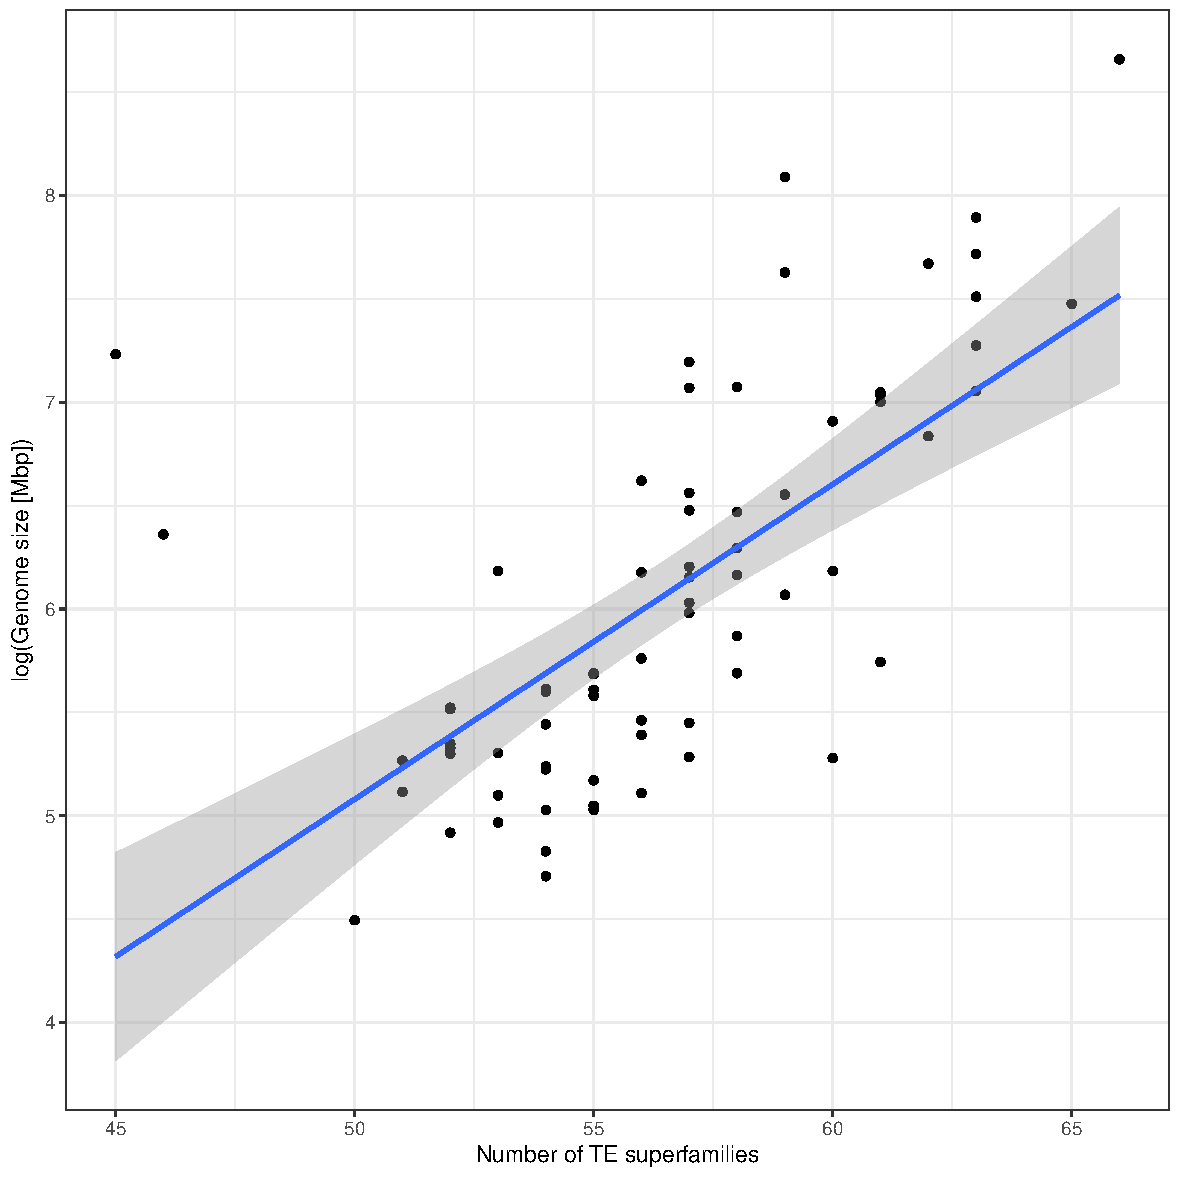
\includegraphics[width=0.7\textwidth]{te-families-vs-genome-size}
\caption[The number of TE superfamilies is significantly correlated to
genome size]{The number of TE superfamilies is significantly correlated to
genome size as well.}
\label{fig:te-families-vs-genome-size}
\end{figure}


\clearpage

\section{Supplementary Tables}

% Please add the following required packages to your document preamble:
% \usepackage{booktabs}
\begin{table}[h]
\caption[Word patterns to exclude non-TE search hits]{{Patterns employed to
exclude non-TE search hits. Note that these are regular expressions for use
with a compatible parser such as GNU grep or Perl.\label{tab:patterns}}}
\centering
\begin{tabular}{@{}l@{}}
\toprule
Pattern               \\ \midrule
transcripta           \\
transpos              \\
gag{[}-/{]}pol        \\
env(elope)? protein   \\
env\textbackslash{}b  \\
pol p(olyp)?rotein    \\
gag(-like)? protein   \\
reverse transcrpitase \\
retro                 \\
integras              \\
replicas              \\
t-element             \\
transporase           \\
piggybac              \\
copia                 \\ \bottomrule
\end{tabular}
\end{table}

% Please add the following required packages to your document preamble:
% \usepackage{booktabs}
\begin{landscape}
\begin{longtable}[]{@{}lllllllll@{}}
\caption[TE coverage data]{{TE coverage by classes in 73 arthropod
genomes.}%
\label{tab:coverage}}

\footnotesize
\endfirsthead

\multicolumn{3}{c}{%
{\tablename\ \thetable{} --continued}} \\
\toprule
Species                    & Genome size & DNA       & LINE      & LTR       & SINE      & Unknown    & Total      & Coverage {[}\%{]} \\ \midrule
\midrule
\endhead

\bottomrule
\endfoot


\toprule
Species                    & Genome size & DNA       & LINE      & LTR       & SINE      & Unknown    & Total      & Coverage {[}\%{]} \\ \midrule
\species{Acromyrmex echinatior}      & 295944863   & 14028877  & 5564391   & 3332023   & 321166    & 56838168   & 80084625   & 27.0606572414132  \\
\species{Acyrthosiphon pisum}        & 541675471   & 46850908  & 7139839   & 2352412   & 38433072  & 44085709   & 138861940  & 25.6356337760031  \\
\species{Aedes aegypti}              & 1383971543  & 284584199 & 170617062 & 74484211  & 19268167  & 224707931  & 773661570  & 55.9015518717208  \\
\species{Agrilus planipennis}        & 353849136   & 11965854  & 20658335  & 7721017   & 805978    & 45704697   & 86855881   & 24.5460203695396  \\
\species{Anopheles gambiae}          & 265011681   & 14556836  & 8430174   & 6904028   & 2383954   & 13962246   & 46237238   & 17.4472452782185  \\
\species{Anoplophora glabripennis}   & 707712193   & 80890038  & 14708125  & 3927741   & 65766     & 193744915  & 293336585  & 41.4485701816925  \\
\species{Apis mellifera}             & 250270657   & 1477978   & 93806     & 661247    & 0         & 8415504    & 10648535   & 4.25480762612934  \\
\species{Athalia rosae}              & 163837890   & 2189910   & 199632    & 415788    & 18659     & 4286428    & 7110417    & 4.33991001715171  \\
\species{Atta cephalotes}            & 317690795   & 14790388  & 3104389   & 1917120   & 80553     & 53276653   & 73169103   & 23.0315464443973  \\
\species{Belgica antarctica}         & 89583723    & 89347     & 225787    & 64091     & 0         & 1927767    & 2306992    & 2.57523568204461  \\
\species{Blattella germanica}        & 2055425512  & 118099518 & 96796661  & 3368694   & 41260001  & 566565387  & 826090261  & 40.1907175023913  \\
\species{Bombus terrestris}          & 248654244   & 3914003   & 2676528   & 1987158   & 9100      & 17941728   & 26528517   & 10.6688374078184  \\
\species{Bombyx mori}                & 481819406   & 14859808  & 52996846  & 2822023   & 45329577  & 66994932   & 183003186  & 37.9816968185794  \\
\species{Camponotus floridanus}      & 232685334   & 3588249   & 1189283   & 1820352   & 245858    & 19473445   & 26317187   & 11.310204449757   \\
\species{Catajapyx silvestris}       & 312272917   & 11564208  & 2999527   & 4563615   & 1450868   & 67274723   & 87852941   & 28.1333846828606  \\
\species{Centruroides exilicauda}    & 931068862   & 60232232  & 19922674  & 2827127   & 40425     & 129049264  & 212071722  & 22.7772327757214  \\
\species{Ceratitis capitata}         & 484773492   & 53984782  & 51057991  & 8093448   & 4481264   & 31292957   & 148910442  & 30.7175298273116  \\
\species{Cimex lectularius}          & 650492763   & 26133805  & 77196299  & 8906041   & 14201408  & 70965264   & 197402817  & 30.346658445453   \\
\species{Copidosoma floridanum}      & 645712421   & 24140234  & 15472247  & 28300530  & 1045178   & 77891713   & 146849902  & 22.7423071361361  \\
\species{Culex quinquefasciatus}     & 579042118   & 148830919 & 19232476  & 12525560  & 10422015  & 82116713   & 273127683  & 47.1688802091595  \\
\species{Danaus plexippus}           & 272853388   & 2556945   & 10476056  & 777496    & 1140231   & 13930574   & 28881302   & 10.5849160282371  \\
\species{Daphnia pulex}              & 197206209   & 3913500   & 1756846   & 11804780  & 1769569   & 20903178   & 40147873   & 20.3583209694985  \\
\species{Drosophila ananassae}       & 230993012   & 5851179   & 18214713  & 36010716  & 5878      & 32843785   & 92926271   & 40.2290399157183  \\
\species{Drosophila erecta}          & 152712140   & 1620381   & 7925820   & 12413050  & 5791      & 6927427    & 28892469   & 18.9195626490468  \\
\species{Drosophila grimshawi}       & 200467819   & 4081630   & 5726513   & 22750394  & 1989      & 7938263    & 40498789   & 20.202139775861   \\
\species{Drosophila melanogaster}    & 143726002   & 1864630   & 6201553   & 14975264  & 0         & 4411181    & 27452628   & 19.1006690633474  \\
\species{Drosophila miranda}         & 136728780   & 1193299   & 2169497   & 932607    & 12128     & 5964753    & 10272284   & 7.5128908485836   \\
\species{Drosophila mojavensis}      & 193826310   & 4423019   & 6200643   & 12547097  & 0         & 15174518   & 38345277   & 19.7833188899897  \\
\species{Drosophila persimilis}      & 188374079   & 3017923   & 10737250  & 21690609  & 44193     & 17715388   & 53205363   & 28.244524555844   \\
\species{Drosophila pseudoobscura}   & 152696384   & 1814141   & 4620512   & 9081564   & 6593      & 7604926    & 23127736   & 15.1462237638843  \\
\species{Drosophila sechellia}       & 166592095   & 4545125   & 10981352  & 16246960  & 0         & 5975207    & 37748644   & 22.6593248617229  \\
\species{Drosophila simulans}        & 124966452   & 454842    & 3082710   & 4363044   & 10511     & 1017167    & 8928274    & 7.14453667933215  \\
\species{Drosophila virilis}         & 206026697   & 2388960   & 7217526   & 14406968  & 2878      & 21536844   & 45553176   & 22.1103267990556  \\
\species{Drosophila willistoni}      & 235516348   & 6979192   & 13395864  & 30867252  & 12943     & 23060371   & 74315622   & 31.5543369413999  \\
\species{Drosophila yakuba}          & 165693946   & 2762860   & 7240428   & 18655858  & 4743      & 8220312    & 36884201   & 22.2604397386975  \\
\species{Ephemera danica}            & 475911277   & 1587870   & 4342127   & 657361    & 5788      & 103286144  & 109879290  & 23.0881879270955  \\
\species{Euperipatoides rowelli}     & 2681872052  & 81520224  & 68827726  & 43632247  & 1743681   & 591339224  & 787063102  & 29.3475261585671  \\
\species{Eurytemora affinis}         & 494890867   & 4913699   & 2873823   & 2975606   & 0         & 118249976  & 129013104  & 26.0690007843689  \\
\species{Frankliniella occidentalis} & 415803855   & 2366622   & 800197    & 769380    & 500775    & 36574762   & 41011736   & 9.86324092642191  \\
\species{Gerris buenoi}              & 1000194699  & 23294121  & 11729071  & 3527948   & 5436752   & 200880060  & 244867952  & 24.4820285735188  \\
\species{Halyomorpha halys}          & 1150099797  & 15071472  & 137983767 & 10173492  & 12033787  & 277888335  & 453150853  & 39.4010027809787  \\
\species{Harpegnathos saltator}      & 294465601   & 22402907  & 4860671   & 2536115   & 401040    & 38188633   & 68389366   & 23.2249083654427  \\
\species{Heliconius melpomene}       & 273786188   & 3309141   & 10787521  & 1806703   & 5675476   & 62279040   & 83857881   & 30.6289669367835  \\
\species{Helicoverpa punctigera}     & 432318525   & 1626618   & 8168605   & 684817    & 14403617  & 49299046   & 74182703   & 17.1592700081497  \\
\species{Homalodisca vitripennis}    & 2247672265  & 33258334  & 50290153  & 1400275   & 5082654   & 223402079  & 313433495  & 13.9448041371814  \\
\species{Hyalella azteca}            & 1181648033  & 17877377  & 22314001  & 1745793   & 6144      & 92142233   & 134085548  & 11.3473339146158  \\
\species{Ixodes scapularis}          & 1765382190  & 50926831  & 55077295  & 19711825  & 11668591  & 568841548  & 706226090  & 40.0041472039547  \\
\species{Ladona fulva}               & 1158111285  & 35625466  & 48467767  & 1277019   & 4772032   & 127344552  & 217486836  & 18.7794419082964  \\
\species{Latrodectus hesperus}       & 1137104758  & 64136256  & 27759711  & 8159512   & 8420167   & 79950721   & 188426367  & 16.570713091678   \\
\species{Leptinotarsa decemlineata}  & 1176182208  & 82875924  & 133162799 & 8299074   & 1354549   & 138863056  & 364555402  & 30.9948067162057  \\
\species{Limnephilus lunatus}        & 1333324643  & 27934987  & 62350860  & 529611    & 28296255  & 293532450  & 412644163  & 30.9485139396767  \\
\species{Limulus polyphemus}         & 1828256766  & 57602361  & 65031258  & 72495679  & 42695658  & 370231034  & 608055990  & 33.2587851612523  \\
\species{Linepithema humile}         & 219500750   & 3146879   & 1635451   & 1634508   & 124443    & 16888693   & 23429974   & 10.6742113637425  \\
\species{Locusta migratoria}         & 5759798599  & 548656473 & 922471727 & 110839523 & 122578589 & 1955778475 & 3660324787 & 63.5495273677711  \\
\species{Loxosceles reclusa}         & 3262503565  & 277060302 & 237214458 & 41355923  & 45464181  & 479023789  & 1080118653 & 33.1070489726806  \\
\species{Lucilia cuprina}            & 470583961   & 6587453   & 19759307  & 7925151   & 2180      & 85424374   & 119698465  & 25.4361548459149  \\
\species{Machilis hrabei}            & 2144866089  & 88401084  & 56089285  & 7823768   & 31164907  & 429393676  & 612872720  & 28.5739386315599  \\
\species{Mayetiola destructor}       & 185827756   & 2334815   & 634675    & 1332276   & 23062     & 14823623   & 19148451   & 10.3044084544615  \\
\species{Mengenilla moldrzyki}       & 155727465   & 11658097  & 2671635   & 5169197   & 18013     & 55690413   & 75207355   & 48.2942138690821  \\
\species{Musca domestica}            & 750403944   & 153293508 & 14279601  & 10470028  & 131797    & 218138285  & 396313219  & 52.8133177029251  \\
\species{Nasonia vitripennis}        & 295780872   & 9357282   & 9442807   & 12159327  & 93355     & 25283154   & 56335925   & 19.0465071723773  \\
\species{Oncopeltus fasciatus}       & 1098693218  & 24473805  & 59736772  & 6583561   & 17420216  & 123890779  & 232105133  & 21.1255634600632  \\
\species{Onthophagus taurus}         & 270546467   & 20788548  & 19283682  & 2900456   & 35890     & 51627557   & 94636133   & 34.9796225577767  \\
\species{Orussus abietinus}          & 201220334   & 2757902   & 424153    & 1413563   & 38403     & 34929859   & 39563880   & 19.6619691526802  \\
\species{Pachypsylla venusta}        & 701795784   & 18682836  & 13497373  & 754417    & 9711493   & 129459210  & 172105329  & 24.5235626835855  \\
\species{Parasteatoda tepidariorum}  & 1443909906  & 71202706  & 13909498  & 2196300   & 34445396  & 332296216  & 454050116  & 31.4458758204544  \\
\species{Pediculus humanus}          & 110781312   & 2419628   & 1040406   & 939937    & 226962    & 2807314    & 7434247    & 6.71074106795197  \\
\species{Pogonomyrmex barbatus}      & 235645958   & 6927372   & 1525631   & 3764006   & 113867    & 18340243   & 30671119   & 13.0157628250089  \\
\species{Solenopsis invicta}         & 396009169   & 15467507  & 7574738   & 8638636   & 0         & 82023961   & 113704842  & 28.7126791248614  \\
\species{Strigamia maritima}         & 176210797   & 2555637   & 1485499   & 20620465  & 342139    & 48848531   & 73852271   & 41.9113199970374  \\
\species{Tribolium castaneum}        & 210248733   & 8676449   & 1786295   & 624856    & 32802     & 32662849   & 43783251   & 20.8245017105525  \\
\species{Trichogramma pretiosum}     & 196221301   & 1988709   & 1912973   & 1512183   & 72212     & 19378013   & 24864090   & 12.671453034551   \\
\species{Zootermopsis nevadensis}    & 485009472   & 14695064  & 26646385  & 236056    & 9305656   & 70248697   & 121131858  & 24.9751530625777  \\ \bottomrule
\end{longtable}
\end{landscape}

\begin{landscape}
\begin{longtable}[]{llp{35em}}
\caption[Genome assembly download URLs]{{Download URLs for the genome
assemblies of 73 arthropod species.}
\label{tab:urls}}

\footnotesize
\endfirsthead

\multicolumn{3}{c}{%
{\tablename\ \thetable{} --continued}} \\
\toprule
Species                     & Order         & URL                                                                                                                                              \\
\midrule
\endhead

\bottomrule
\endfoot

\toprule
Species                     & Order         & URL                                                                                                                                              \\ 
\midrule
\species{Aedes aegypti}                 & Diptera       & \url{ftp://ftp.ncbi.nlm.nih.gov/genomes/all/GCA\_000004015.1\_Aedes\_aegypti/GCA\_000004015.1\_Aedes\_aegypti\_genomic.fna.gz}                         \\
\species{Atta cephalotes}               & Hymenoptera   & \url{ftp://ftp.ncbi.nlm.nih.gov/genomes/all/GCA\_000143395.2\_Attacep1.0/GCA\_000143395.2\_Attacep1.0\_genomic.fna.gz}                                 \\
\species{Acromyrmex echinatior}         & Hymenoptera   & \url{ftp://ftp.ncbi.nlm.nih.gov/genomes/all/GCA\_000204515.1\_Aech\_3.9/GCA\_000204515.1\_Aech\_3.9\_genomic.fna.gz}                                   \\
\species{Anopheles gambiae}             & Diptera       & \url{ftp://ftp.ncbi.nlm.nih.gov/genomes/all/GCA\_000005575.1\_AgamP3/GCA\_000005575.1\_AgamP3\_genomic.fna.gz}                                         \\
\species{Apis mellifera}                & Hymenoptera   & \url{ftp://ftp.ncbi.nlm.nih.gov/genomes/all/GCA\_000002195.1\_Amel\_4.5/GCA\_000002195.1\_Amel\_4.5\_genomic.fna.gz}                                   \\
\species{Acyrthosiphon pisum}           & Hemiptera     & \url{ftp://ftp.ncbi.nlm.nih.gov/genomes/all/GCA\_000142985.2\_Acyr\_2.0/GCA\_000142985.2\_Acyr\_2.0\_genomic.fna.gz}                                   \\
\species{Belgica antarctica}            & Diptera       & \url{ftp://ftp.ncbi.nlm.nih.gov/genomes/all/GCA\_000775305.1\_ASM77530v1/GCA\_000775305.1\_ASM77530v1\_genomic.fna.gz}                                 \\
\species{Bombyx mori}                   & Lepidoptera   & \url{ftp://ftp.ncbi.nlm.nih.gov/genomes/all/GCF\_000151625.1\_ASM15162v1/GCF\_000151625.1\_ASM15162v1\_genomic.fna.gz}                                 \\
\species{Bombus terrestris}             & Hymenoptera   & \url{ftp://ftp.ncbi.nlm.nih.gov/genomes/all/GCA\_000214255.1\_Bter\_1.0/GCA\_000214255.1\_Bter\_1.0\_genomic.fna.gz}                                   \\
\species{Camponotus floridanus}         & Hymenoptera   & \url{ftp://ftp.ncbi.nlm.nih.gov/genomes/all/GCA\_000147175.1\_CamFlo\_1.0/GCA\_000147175.1\_CamFlo\_1.0\_genomic.fna.gz}                               \\
\species{Culex quinquefasciatus}        & Diptera       & \url{ftp://ftp.ncbi.nlm.nih.gov/genomes/all/GCA\_000209185.1\_CulPip1.0/GCA\_000209185.1\_CulPip1.0\_genomic.fna.gz}                                   \\
\species{Drosophila ananassae}          & Diptera       & \url{ftp://ftp.ncbi.nlm.nih.gov/genomes/all/GCF\_000005115.1\_dana\_caf1/GCF\_000005115.1\_dana\_caf1\_genomic.fna.gz}                                 \\
\species{Drosophila erecta}             & Diptera       & \url{ftp://ftp.ncbi.nlm.nih.gov/genomes/all/GCF\_000005135.1\_dere\_caf1/GCF\_000005135.1\_dere\_caf1\_genomic.fna.gz}                                 \\
\species{Drosophila grimshawi}          & Diptera       & \url{ftp://ftp.ncbi.nlm.nih.gov/genomes/all/GCF\_000005155.2\_dgri\_caf1/GCF\_000005155.2\_dgri\_caf1\_genomic.fna.gz}                                 \\
\species{Drosophila melanogaster}       & Diptera       & \url{ftp://ftp.ncbi.nlm.nih.gov/genomes/all/GCA\_000001215.4\_Release\_6\_plus\_ISO1\_MT/GCA\_000001215.4\_Release\_6\_plus\_ISO1\_MT\_genomic.fna.gz} \\
\species{Drosophila miranda}            & Diptera       & \url{ftp://ftp.ncbi.nlm.nih.gov/genomes/all/GCA\_000269505.2\_DroMir\_2.2/GCA\_000269505.2\_DroMir\_2.2\_genomic.fna.gz}                               \\
\species{Drosophila mojavensis}         & Diptera       & \url{ftp://ftp.ncbi.nlm.nih.gov/genomes/all/GCF\_000005175.2\_dmoj\_caf1/GCF\_000005175.2\_dmoj\_caf1\_genomic.fna.gz}                                 \\
\species{Drosophila persimilis}         & Diptera       & \url{ftp://ftp.ncbi.nlm.nih.gov/genomes/all/GCF\_000005195.2\_dper\_caf1/GCF\_000005195.2\_dper\_caf1\_genomic.fna.gz}                                 \\
\species{Danaus plexippus}              & Lepidoptera   & \url{ftp://ftp.ncbi.nlm.nih.gov/genomes/all/GCA\_000235995.1\_DanPle\_1.0/GCA\_000235995.1\_DanPle\_1.0\_genomic.fna.gz}                               \\
\species{Drosophila pseudoobscura}      & Diptera       & \url{ftp://ftp.ncbi.nlm.nih.gov/genomes/all/GCF\_000001765.3\_Dpse\_3.0/GCF\_000001765.3\_Dpse\_3.0\_genomic.fna.gz}                                   \\
\species{Daphnia pulex}                 & Cladocera     & \url{ftp://ftp.ncbi.nlm.nih.gov/genomes/all/GCA\_000187875.1\_V1.0/GCA\_000187875.1\_V1.0\_genomic.fna.gz}                                             \\
\species{Drosophila sechellia}          & Diptera       & \url{ftp://ftp.ncbi.nlm.nih.gov/genomes/all/GCF\_000005215.3\_dsec\_caf1/GCF\_000005215.3\_dsec\_caf1\_genomic.fna.gz}                                 \\
\species{Drosophila simulans}           & Diptera       & \url{ftp://ftp.ncbi.nlm.nih.gov/genomes/all/GCA\_000754195.2\_ASM75419v2/GCA\_000754195.2\_ASM75419v2\_genomic.fna.gz}                                 \\
\species{Drosophila virilis}            & Diptera       & \url{ftp://ftp.ncbi.nlm.nih.gov/genomes/all/GCF\_000005245.1\_dvir\_caf1/GCF\_000005245.1\_dvir\_caf1\_genomic.fna.gz}                                 \\
\species{Drosophila willistoni}         & Diptera       & \url{ftp://ftp.ncbi.nlm.nih.gov/genomes/all/GCF\_000005925.1\_dwil\_caf1/GCF\_000005925.1\_dwil\_caf1\_genomic.fna.gz}                                 \\
\species{Drosophila yakuba}             & Diptera       & \url{ftp://ftp.ncbi.nlm.nih.gov/genomes/all/GCA\_000005975.1\_dyak\_caf1/GCA\_000005975.1\_dyak\_caf1\_genomic.fna.gz}                                 \\
\species{Heliconius melpomene}          & Lepidoptera   & \url{ftp://ftp.ncbi.nlm.nih.gov/genomes/all/GCA\_000313835.2\_ASM31383v2/GCA\_000313835.2\_ASM31383v2\_genomic.fna.gz}                                 \\
\species{Harpegnathos saltator}         & Hymenoptera   & \url{ftp://ftp.ncbi.nlm.nih.gov/genomes/all/GCA\_000147195.1\_HarSal\_1.0/GCA\_000147195.1\_HarSal\_1.0\_genomic.fna.gz}                               \\
\species{Ixodes scapularis}             & Ixodida       & \url{ftp://ftp.ncbi.nlm.nih.gov/genomes/all/GCA\_000208615.1\_JCVI\_ISG\_i3\_1.0/GCA\_000208615.1\_JCVI\_ISG\_i3\_1.0\_genomic.fna.gz}                 \\
\species{Linepithema humile}            & Hymenoptera   & \url{ftp://ftp.ncbi.nlm.nih.gov/genomes/all/GCA\_000217595.1\_Lhum\_UMD\_V04/GCA\_000217595.1\_Lhum\_UMD\_V04\_genomic.fna.gz}                         \\
\species{Locusta migratoria}            & Orthoptera    & \url{ftp://ftp.ncbi.nlm.nih.gov/genomes/all/GCA\_000516895.1\_LocustGenomeV1/GCA\_000516895.1\_LocustGenomeV1\_genomic.fna.gz}                         \\
\species{Limulus polyphemus}            & Xiphosura     & \url{ftp://ftp.ncbi.nlm.nih.gov/genomes/all/GCA\_000517525.1\_Limulus\_polyphemus-2.1.2/GCA\_000517525.1\_Limulus\_polyphemus-2.1.2\_genomic.fna.gz}   \\
\species{Mayetiola destructor}          & Diptera       & \url{ftp://ftp.ncbi.nlm.nih.gov/genomes/all/GCA\_000149185.1\_Mdes\_1.0/GCA\_000149185.1\_Mdes\_1.0\_genomic.fna.gz}                                   \\
\species{Musca domestica}               & Diptera       & \url{ftp://ftp.ncbi.nlm.nih.gov/genomes/all/GCF\_000371365.1\_Musca\_domestica-2.0.2/GCF\_000371365.1\_Musca\_domestica-2.0.2\_genomic.fna.gz}         \\
\species{Mengenilla moldrzyki}          & Strepsiptera  & \url{ftp://ftp.ncbi.nlm.nih.gov/genomes/all/GCA\_000281935.1\_Memo\_1.0/GCA\_000281935.1\_Memo\_1.0\_genomic.fna.gz}                                   \\
\species{Nasonia vitripennis}           & Hymenoptera   & \url{ftp://ftp.ncbi.nlm.nih.gov/genomes/all/GCA\_000002325.2\_Nvit\_2.1/GCA\_000002325.2\_Nvit\_2.1\_genomic.fna.gz}                                   \\
\species{Pogonomyrmex barbatus}         & Hymenoptera   & \url{ftp://ftp.ncbi.nlm.nih.gov/genomes/all/GCA\_000187915.1\_Pbar\_UMD\_V03/GCA\_000187915.1\_Pbar\_UMD\_V03\_genomic.fna.gz}                         \\
\species{Pediculus humanus}             & Phthiraptera  & \url{ftp://ftp.ncbi.nlm.nih.gov/genomes/all/GCA\_000006295.1\_JCVI\_LOUSE\_1.0/GCA\_000006295.1\_JCVI\_LOUSE\_1.0\_genomic.fna.gz}                     \\
\species{Solenopsis invicta}            & Hymenoptera   & \url{ftp://ftp.ncbi.nlm.nih.gov/genomes/all/GCA\_000188075.1\_Si\_gnG/GCA\_000188075.1\_Si\_gnG\_genomic.fna.gz}                                       \\
\species{Strigamia maritima}            & Myriapoda     & \url{ftp://ftp.ncbi.nlm.nih.gov/genomes/all/GCA\_000239455.1\_Smar\_1.0/GCA\_000239455.1\_Smar\_1.0\_genomic.fna.gz}                                   \\
\species{Tribolium castaneum}           & Coleoptera    & \url{ftp://ftp.ncbi.nlm.nih.gov/genomes/all/GCA\_000002335.2\_Tcas\_3.0/GCA\_000002335.2\_Tcas\_3.0\_genomic.fna.gz}                                   \\
\species{Zootermopsis nevadensis}       & Isoptera      & \url{ftp://ftp.ncbi.nlm.nih.gov/genomes/all/GCA\_000696155.1\_ZooNev1.0/GCA\_000696155.1\_ZooNev1.0\_genomic.fna.gz}                                   \\
\species{Agrilus planipennis} Fairmaire & Coleoptera    & \url{ftp://ftp.hgsc.bcm.edu/I5K-pilot/Emerald\_ash\_borer/NCBI-submitted/Aplan.agp.contamination-free.scaffolds.50.fa}                                 \\
\species{Anoplophora glabripennis}      & Coleoptera    & \url{ftp://ftp.hgsc.bcm.edu/I5K-pilot/Asian\_long-horned\_beetle/Agla\_Btl03082013.genome.fa}                                                          \\
\species{Athalia rosae}                 & Hymenoptera   & \url{ftp://ftp.hgsc.bcm.edu/I5K-pilot/Turnip\_sawfly/Aros01112013-genome.fa}                                                                           \\
\species{Blattella germanica}           & Blattodea     & \url{ftp://ftp.hgsc.bcm.edu/I5K-pilot/German\_cockroach/Bgermanica.scaffolds}                                                                          \\
\species{Catajapyx silvestris}          & Diplura       & \url{ftp://ftp.hgsc.bcm.edu/I5K-pilot/Silvestris\_Northern\_Forcepstail/forcepstail.consistent.scaffolds}                                              \\
\species{Centruroides exilicauda}       & Scorpiones    & \url{ftp://ftp.hgsc.bcm.edu/I5K-pilot/Bark\_scorpion/NCBI-submitted/Cscul.scaffolds.50.fa}                                                             \\
\species{Ceratitis capitata}            & Diptera       & \url{ftp://ftp.hgsc.bcm.edu/I5K-pilot/Mediterranean\_fruit\_fly/Ccap01172013-genome.fa}                                                                \\
\species{Cimex lectularius}             & Hemiptera     & \url{ftp://ftp.hgsc.bcm.edu/I5K-pilot/Bed\_bug/Clec\_Bbug02212013.genome.fa}                                                                           \\
\species{Copidosoma floridanum}         & Hymenoptera   & \url{ftp://ftp.hgsc.bcm.edu/I5K-pilot/Copidosoma\_floridanum/NCBI-submitted/Cflo.scaffolds.50.fa}                                                      \\
\species{Ephemera danica}               & Ephemeroptera & \url{ftp://ftp.hgsc.bcm.edu/I5K-pilot/Mayfly/Edan07162013.scaffolds.fa}                                                                                \\
\species{Euperipatoides rowelli}        & Euonychophora & \url{ftp://ftp.hgsc.bcm.edu/I5K-pilot/Velvet\_worm/pre\_assembly/Erow.scaffolds.fasta}                                                                 \\
\species{Eurytemora affinis}            & Calanoida     & \url{ftp://ftp.hgsc.bcm.edu/I5K-pilot/Eurytemora\_affinis/NCBI-submitted/Eaff\_11172013.genome.fa}                                                     \\
\species{Frankliniella occidentalis}    & Thysanoptera  & \url{ftp://ftp.hgsc.bcm.edu/I5K-pilot/Western\_flower\_thrips/NCBI-submitted/Focc.scaffolds}                                                           \\
\species{Gerris buenoi}                 & Hemiptera     & \url{ftp://ftp.hgsc.bcm.edu/I5K-pilot/Water\_strider/NCBI-submitted/Gbue\_1.0-unplaced\_scaffolds.fsa}                                                 \\
\species{Halyomorpha halys}             & Hemiptera     & \url{ftp://ftp.hgsc.bcm.edu/I5K-pilot/Brown\_marmorated\_stink\_bug/Hhal.scaffolds.fa}                                                                 \\
\species{Helicoverpa punctigera}        & Lepidoptera   & \url{ftp://ftp.hgsc.bcm.edu/I5K-pilot/Helicoverpa\_punctigera/Hpun12202012.genome.fa}                                                                  \\
\species{Homalodisca vitripennis}       & Hemiptera     & \url{ftp://ftp.hgsc.bcm.edu/I5K-pilot/Glassy-winged\_sharpshooter/NCBI-submitted/Hvit.scaffolds}                                                       \\
\species{Hyalella azteca}               & Amphipoda     & \url{ftp://ftp.hgsc.bcm.edu/I5K-pilot/Hyalella\_azteca/pre\_assembly/Hazt.scaffolds.fasta}                                                             \\
\species{Ladona fulva}                  & Odonata       & \url{ftp://ftp.hgsc.bcm.edu/I5K-pilot/Scarce\_Chaser/Lful\_Scha04012013-genome.fa}                                                                     \\
\species{Latrodectus hesperus}          & Araneae       & \url{ftp://ftp.hgsc.bcm.edu/I5K-pilot/Western\_black\_widow\_spider/NCBI-submitted/Lhes.scaffolds}                                                     \\
\species{Leptinotarsa decemlineata}     & Coleoptera    & \url{ftp://ftp.hgsc.bcm.edu/I5K-pilot/Colorado\_Potato\_Beetle/Ldec.genome.10062013.fa}                                                                \\
\species{Limnephilus lunatus}           & Trichoptera   & \url{ftp://ftp.hgsc.bcm.edu/I5K-pilot/Caddisfly/NCBI-submitted/Llun.contaminationfree.scaffolds.fa}                                                    \\
\species{Loxosceles reclusa}            & Araneae       & \url{ftp://ftp.hgsc.bcm.edu/I5K-pilot/Brown\_recluse\_spider/NCBI-submitted/Lrec.scaffolds}                                                            \\
\species{Lucilia cuprina}               & Diptera       & \url{ftp://ftp.hgsc.bcm.edu/I5K-pilot/Sheep\_blowfly/NCBIsubmitted/Lcup.scaffolds}                                                                     \\
\species{Machilis hrabei}               & Archaeognatha & \url{ftp://ftp.hgsc.bcm.edu/I5K-pilot/Hrabes\_jumping\_bristletail/pre-assembly/Mhar.scaffolds.fasta}                                                  \\
\species{Oncopeltus fasciatus}          & Hemiptera     & \url{ftp://ftp.hgsc.bcm.edu/I5K-pilot/Milkweed\_bug/NCBI-submitted/Ofas.contaminationfree.scaffolds}                                                   \\
\species{Onthophagus taurus}            & Coleoptera    & \url{ftp://ftp.hgsc.bcm.edu/I5K-pilot/Bull-headed\_Dung\_beetle/Otaur.scaffolds.fa}                                                                    \\
\species{Orussus abietinus}             & Hymenoptera   & \url{ftp://ftp.hgsc.bcm.edu/I5K-pilot/Parasitic\_wood\_wasp/Oabi11242013.genome.fa}                                                                    \\
\species{Pachypsylla venusta}           & Hemiptera     & \url{ftp://ftp.hgsc.bcm.edu/I5K-pilot/Hackberry\_petiole\_gall\_psyllid/NCBI-submitted/Pven.scaffolds.50.fa}                                           \\
\species{Parasteatoda tepidariorum}     & Araneae       & \url{ftp://ftp.hgsc.bcm.edu/I5K-pilot/Common\_house\_spider/NCBI-submitted/Ptep01282013.genome.fa}                                                     \\
\species{Trichogramma pretiosum}        & Hymenoptera   & \url{ftp://ftp.hgsc.bcm.edu/I5K-pilot/Trichogramma\_pretiosum/Tpre\_scaffolds.50.fa}                                                                   \\
\end{longtable}
\end{landscape}

	\chapter{Supplemental material to chapter \ref{cha:dynamics}}

\paragraph{Supplemental Figures:}

\begin{itemize}
	\item Figure \ref{fig:agesplit}: Most insect TEs are clade-specific (page \pageref{fig:agesplit})
	\item Figure \ref{fig:loss-coefficient}: DNA loss coefficient correlations, with and without PIC (page \pageref{fig:loss-coefficient})
	\item Figure \ref{fig:te-content-vs-size}: TE content is a predictor for genome size (page \pageref{fig:te-content-vs-size})
	\item Figure \ref{fig:loss-coefficient-plots-flight}: TE content is a predictor for genome size, irrespective of flight ability (page \pageref{fig:loss-coefficient-plots-flight})
	\item Figure \ref{fig:ancient-lineage-specific}: TE age classification explanation (page \pageref{fig:ancient-lineage-specific})
\end{itemize}

\paragraph{Supplemental Tables:}

\begin{itemize}
	\item Table \ref{tab:genome-assemblies}: NCBI accession numbers and references for the genome assemblies (page \pageref{tab:genome-assemblies})
	\item Table \ref{tab:genome-size-estimates}: Genome size estimates (page \pageref{tab:genome-size-estimates})
	\item Table \ref{tab:species-not-in-bold-but-in-tree}: Species not represented in BOLD database (page \pageref{tab:species-not-in-bold-but-in-tree})
	\item Table \ref{tab:species-divergence-times}: Divergence times and MRCA splits (page \pageref{tab:species-divergence-times})
	\item Table \ref{tab:gain-loss}: DNA gain and loss (page \pageref{tab:gain-loss})
	\item Table \ref{tab:order-divergence-times}: Divergence times and clade-specific substitution rates (page \pageref{tab:order-divergence-times})
	\item Table \ref{tab:calibration-points}: Branch length calibration points from Misof et al. (2014) (page \pageref{tab:calibration-points})
	\item Table \ref{tab:phylogeny-sources}: Literature sources for the constraint phylogeny (page \pageref{tab:phylogeny-sources})
	\item Table \ref{tab:genome-size-spread}: Genome size spread in Eukaryotes (page \pageref{tab:genome-size-spread})
\end{itemize}


\section{Supplemental figures}

\begin{figure}[h!]
\centering
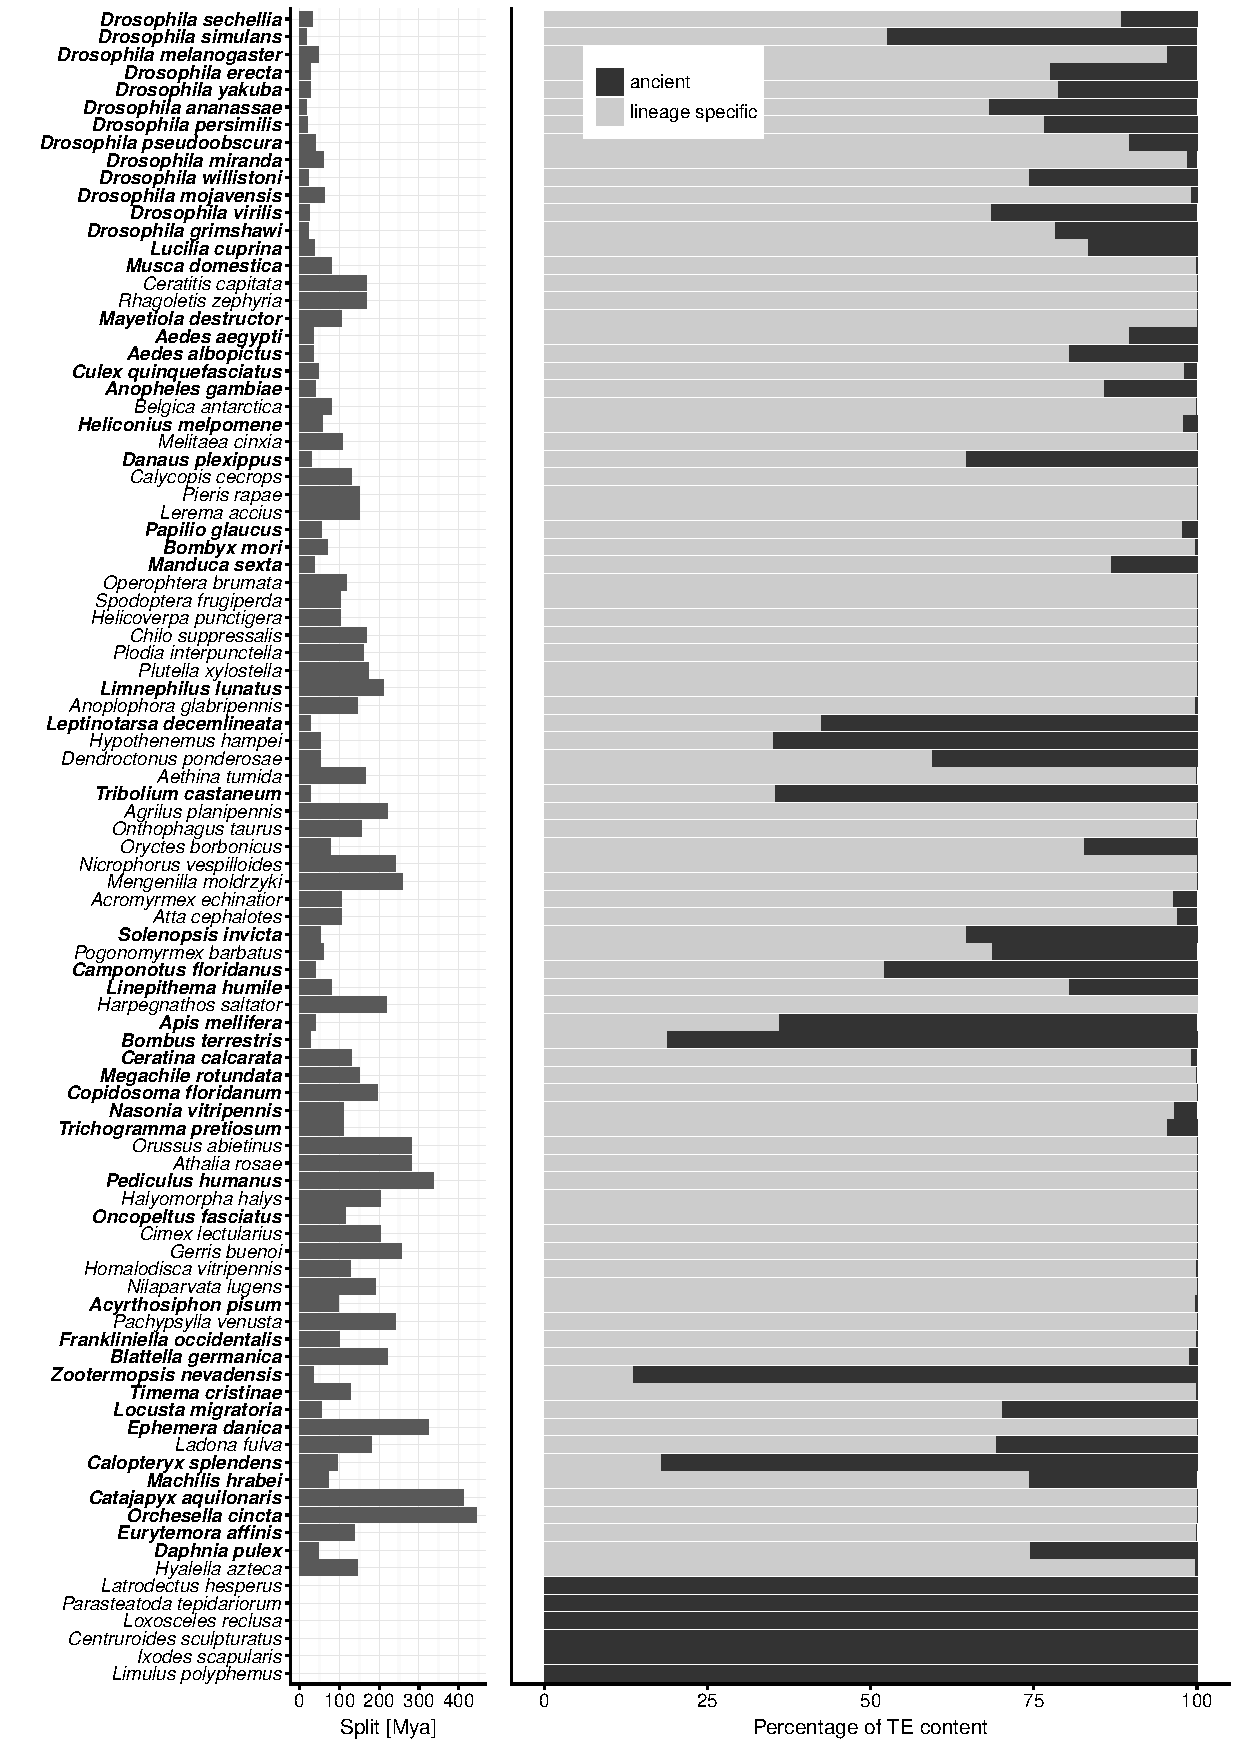
\includegraphics[width=\textwidth]{agesplit+ages}
\caption[Most insect TEs are clade-specific]{Most insect transposable elements are clade-specific when analyzed at order level. TE age was determined from the RepeatMasker \citep{Smit2015} annotation using the intra-TE-family Kimura distances and order-specific nucleotide substitution rates based on data from \citet{Misof2014}. TE copies were classified as ``ancient'' if they were older (more divergent) than the clade the host belongs to. Bold font face denotes species for which ancestral genome size inferences and branch length estimates are available.}
\label{fig:agesplit}
\end{figure}

\begin{figure}[h!]
\centering
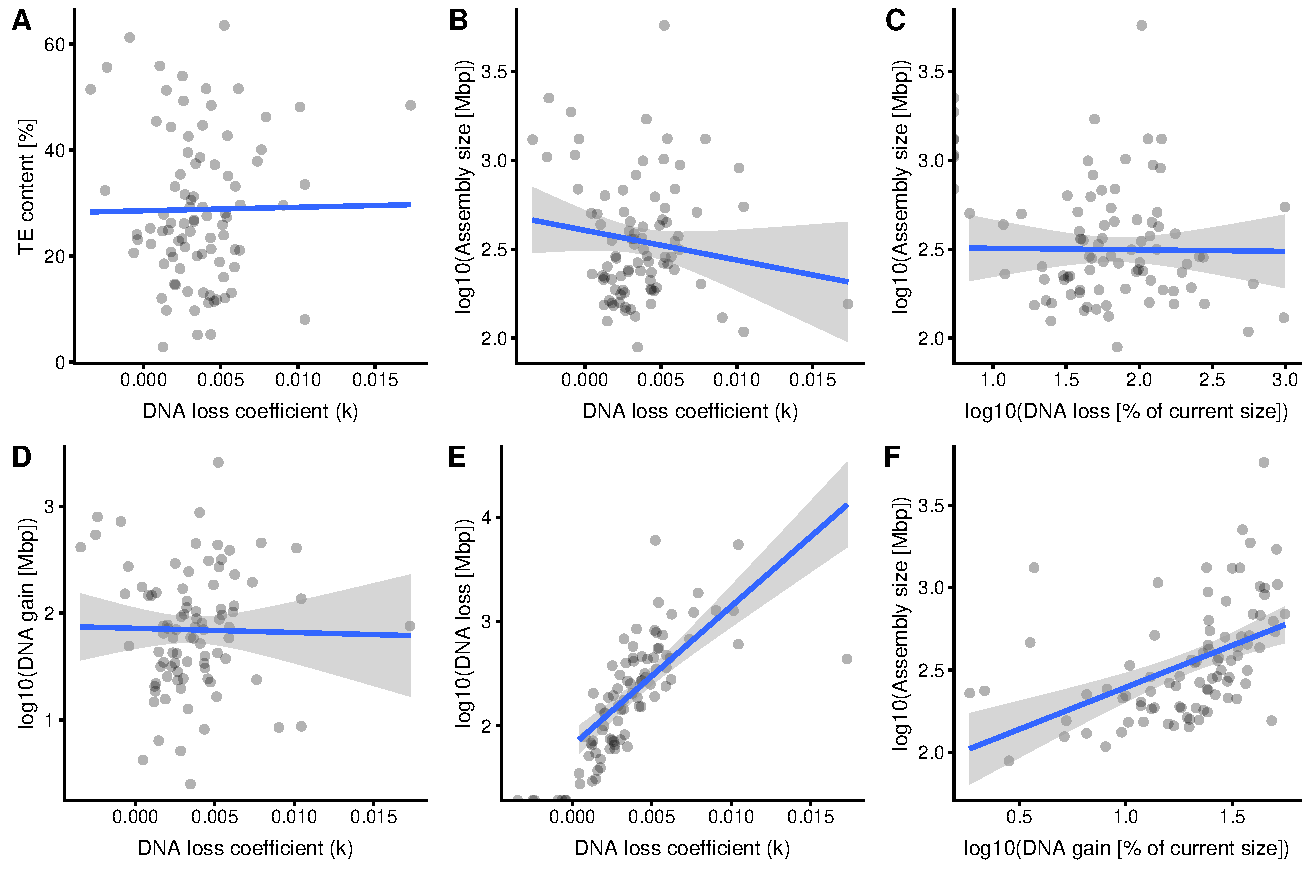
\includegraphics[width=\textwidth]{loss-coefficient-plots}
\rule{\textwidth}{0.2pt}

\bigskip

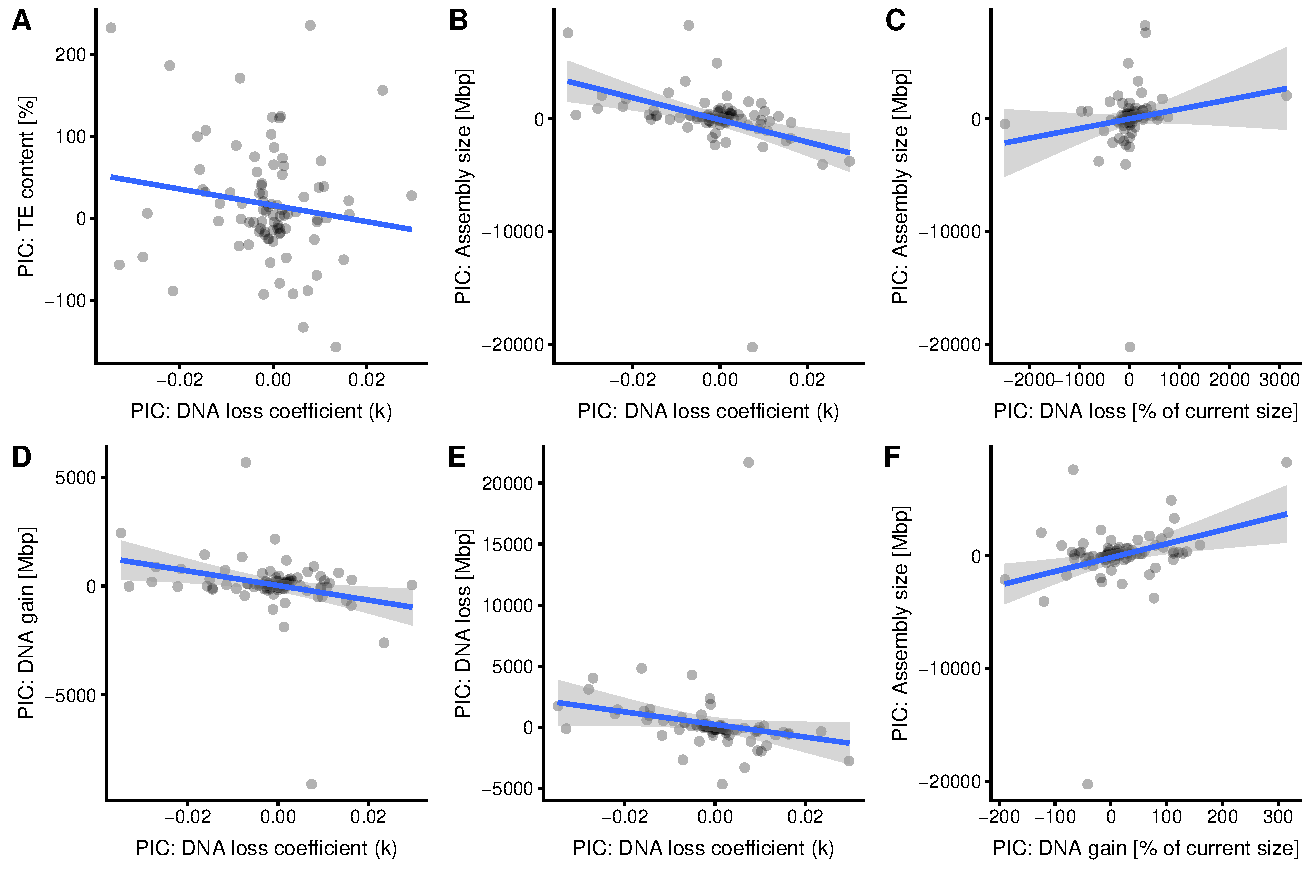
\includegraphics[width=\textwidth]{loss-coefficient-plots-PICs}
\caption[DNA loss coefficient correlations, with and without PIC]{Insect genome size dynamics and TE content are governed by the DNA loss coefficient. Top: without phylogenetic independent contrasts (PIC), bottom: with PIC. A: While TE content determines the genome size (Figure \ref{fig:te-content-vs-size}), the TE content is not dependent on the DNA loss coefficient $k$. There is no correlation despite a visible trend in the regression (Pearson, $p = 0.15$). Obviously, genome (assembly) size decreases with higher $k$ (B, $p = 0.0002$), as does the amount of DNA gained (D, $p = 0.01$). Surprisingly, the assembly size appears to remain more or less stable despite increasing amounts of DNA loss (C). A strong negative correlation is, however, found by testing for it (section \ref{sec:correlation-tests}; $p \ll 0.005$).}
\label{fig:loss-coefficient}
\end{figure}

\begin{figure}
\centering
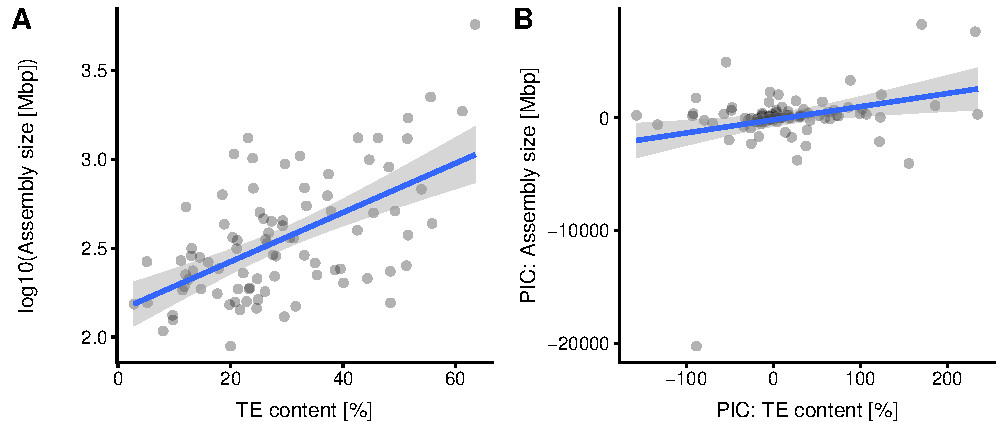
\includegraphics[width=\textwidth]{te-content-vs-size}
\caption[TE content is a predictor for genome size]{TE content is a predictor for genome size. Dots: individual measurements; blue line: linear regression; shaded area: confidence interval. PIC: phylogenetic independent contrast \citep{Felsenstein1985}}
\label{fig:te-content-vs-size}
\end{figure}

\begin{figure}[h!]
\centering
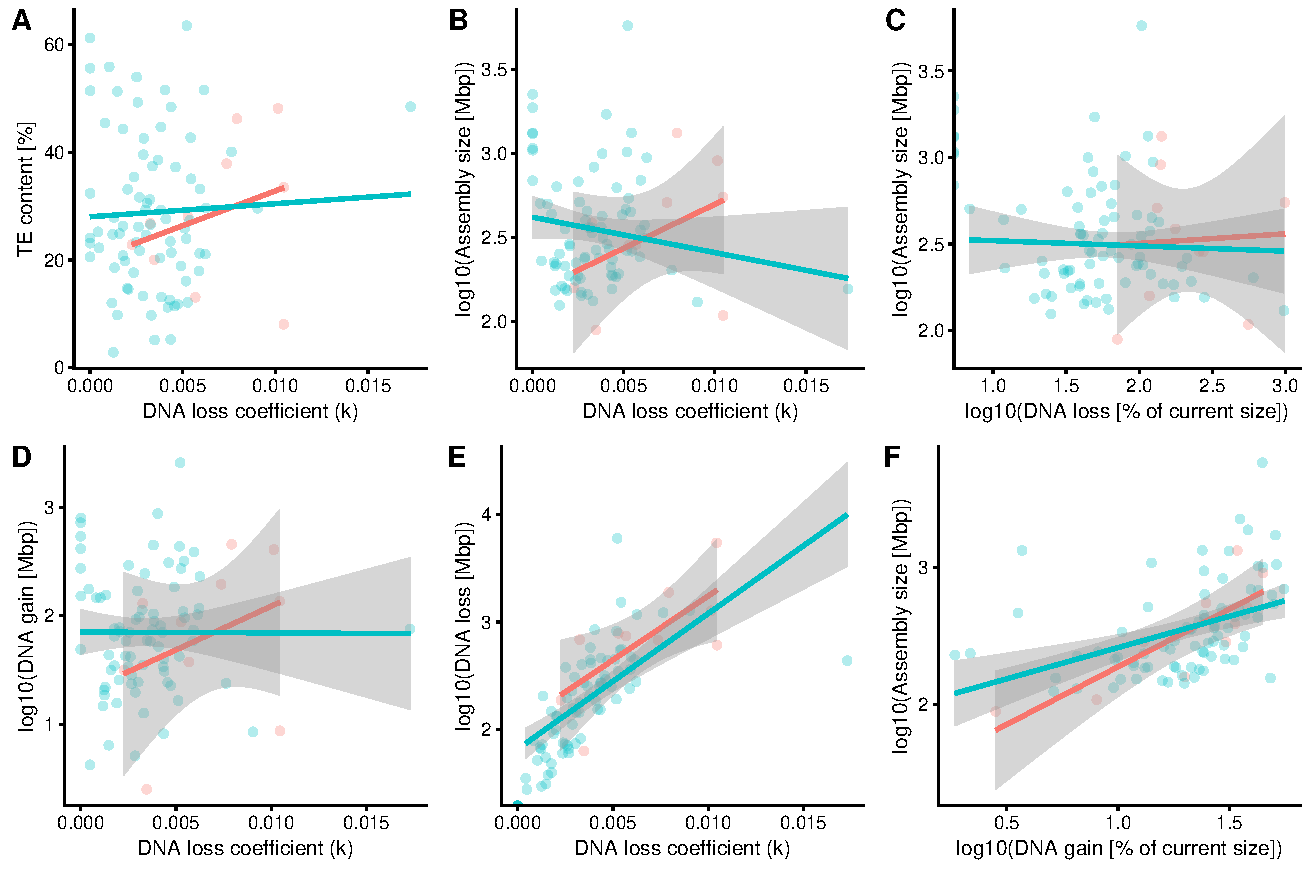
\includegraphics[width=\textwidth]{loss-coeffi-flightless}
\caption[TE content is a predictor for genome size, irrespective of flight ability]{The same as Fig. \ref{fig:te-content-vs-size}. Red: flightless; blue: flying}
\label{fig:loss-coefficient-plots-flight}
\end{figure}

\begin{figure}[h!]
\centering
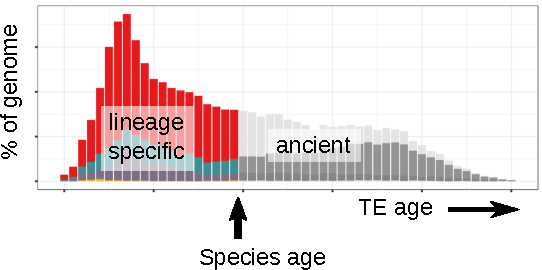
\includegraphics[width=\textwidth]{ancient-lineage-specific}
\caption[TE age classification explanation]{The age classification analysis splits the repeat landscape into the ancestral and the lineage-specific parts. The further to the right the species' age is, the greater the lineage-specific fraction of the TE content. If the species is older than the oldest TE copy on the landscape, it will have 0 \% ancestral TEs.}
\label{fig:ancient-lineage-specific}
\end{figure}

\clearpage

\section{Data sources}

\subsection{Genome assemblies}

\begin{center}
\tabcolsep=3pt
\begin{longtable}{lllp{12em}}
\caption[NCBI accession numbers and references for the genome assemblies]{NCBI accession numbers and references for the genome assemblies.} \label{tab:genome-assemblies} \\

\footnotesize
\endfirsthead

\multicolumn{2}{c}{%
{\tablename\ \thetable{} --continued}} \\
\toprule
Species & Order  & NCBI Accession & Reference \\
\midrule
\endhead

\bottomrule
\endfoot


\toprule
Species                              & Order           & NCBI Accession   & Reference \\
\midrule
\species{Drosophila yakuba}          & Diptera         & GCA\_000005975.1 & \citet{Drosophila12GenomesConsortium2007} \\
\species{Drosophila simulans}        & Diptera         & GCA\_000754195.2 & \citet{Drosophila12GenomesConsortium2007} \\
\species{Drosophila sechellia}       & Diptera         & GCF\_000005215.3 & \citet{Drosophila12GenomesConsortium2007} \\
\species{Drosophila melanogaster}    & Diptera         & GCA\_000001215.4 & \citet{Adams2000} \\
\species{Drosophila erecta}          & Diptera         & GCF\_000005135.1 & \citet{Drosophila12GenomesConsortium2007} \\
\species{Drosophila ananassae}       & Diptera         & GCF\_000005115.1 & \citet{Drosophila12GenomesConsortium2007} \\
\species{Drosophila pseudoobscura}   & Diptera         & GCF\_000001765.3 & \citet{Drosophila12GenomesConsortium2007} \\
\species{Drosophila persimilis}      & Diptera         & GCF\_000005195.2 & \citet{Drosophila12GenomesConsortium2007} \\
\species{Drosophila miranda}         & Diptera         & GCA\_000269505.2 & \citet{McGaugh2012} \\
\species{Drosophila willistoni}      & Diptera         & GCF\_000005925.1 & \citet{Drosophila12GenomesConsortium2007} \\
\species{Drosophila virilis}         & Diptera         & GCF\_000005245.1 & \citet{Drosophila12GenomesConsortium2007} \\
\species{Drosophila mojavensis}      & Diptera         & GCF\_000005175.2 & \citet{Drosophila12GenomesConsortium2007} \\
\species{Drosophila grimshawi}       & Diptera         & GCF\_000005155.2 & \citet{Drosophila12GenomesConsortium2007} \\
\species{Rhagoletis zephyria}        & Diptera         & GCA\_001687245.1 & \citet{Drosophila12GenomesConsortium2007} \\
\species{Ceratitis capitata}         & Diptera         & GCA\_000347755.2 & \citet{Papanicolaou2016} \\
\species{Lucilia cuprina}            & Diptera         & GCA\_000699065.1 & i5k Initiative \\
\species{Musca domestica}            & Diptera         & GCF\_000371365.1 & \citet{Scott2014} \\
\species{Culex quinquefasciatus}     & Diptera         & GCA\_000209185.1 & \citet{Arensburger2010} \\
\species{Aedes albopictus}           & Diptera         & GCA\_001444175.2 & \citet{Chen2015} \\
\species{Aedes aegypti}              & Diptera         & GCA\_000004015.1 & \citet{Nene2007} \\
\species{Anopheles gambiae}          & Diptera         & GCA\_000005575.1 & \citet{Holt2002} \\
\species{Belgica antarctica}         & Diptera         & GCA\_000775305.1 & \citet{Kelley2014} \\
\species{Mayetiola destructor}       & Diptera         & GCA\_000149185.1 & \citet{Zhao2015} \\
\species{Papilio glaucus}            & Lepidoptera     & GCA\_000931545.1 & \citet{Cong2015} \\
\species{Melitaea cinxia}            & Lepidoptera     & GCA\_000716385.1 & \citet{Ahola2014} \\
\species{Heliconius melpomene}       & Lepidoptera     & GCA\_000313835.2 & \citet{TheHeliconiusGenomeConsortium2012} \\
\species{Danaus plexippus}           & Lepidoptera     & GCA\_000235995.1 & \citet{Zhan2011} \\
\species{Calycopis cecrops}          & Lepidoptera     & GCA\_001625245.1 & \citet{Cong2016} \\
\species{Pieris rapae}               & Lepidoptera     & GCA\_001856805.1 & \citet{Shen2016} \\
\species{Lerema accius}              & Lepidoptera     & GCA\_001278395.1 & \citet{Cong2015a} \\
\species{Manduca sexta}              & Lepidoptera     & GCA\_000262585.1 & \citet{Kanost2016} \\
\species{Plutella xylostella}        & Lepidoptera     & GCA\_000325945.1 & \citet{You2013} \\
\species{Spodoptera frugiperda}      & Lepidoptera     & GCA\_000753635.2 & \citet{Gouin2017} \\
\species{Helicoverpa punctigera}     & Lepidoptera     &                  & i5k Initiative \\
\species{Chilo suppressalis}         & Lepidoptera     & GCA\_000636095.1 & \citet{Yin2014} \\
\species{Operophtera brumata}        & Lepidoptera     & GCA\_001266575.1 & \citet{Derks2015} \\
\species{Plodia interpunctella}      & Lepidoptera     & GCA\_900182495.1 & \citet{Paterson2017} \\
\species{Bombyx mori}                & Lepidoptera     & GCF\_000151625.1 & \citet{InternationalSilkwormGenomeConsortium2008} \\
\species{Limnephilus lunatus}        & Trichoptera     & GCA\_000648945.1 & i5k Initiative \\
\species{Aethina tumida}             & Coleoptera      & GCF\_001937115.1 & \citet{Evans2018} \\
\species{Anoplophora glabripennis}   & Coleoptera      & GCA\_000390285.1 & i5k Initiative \\
\species{Leptinotarsa decemlineata}  & Coleoptera      & GCA\_000500325.1 & i5k Initiative \\
\species{Tribolium castaneum}        & Coleoptera      & GCA\_000002335.2 & \citet{TriboliumGenomeSequencingConsortium2008} \\
\species{Agrilus planipennis}        & Coleoptera      & GCA\_000699045.1 & i5k Initiative \\
\species{Oryctes borbonicus}         & Coleoptera      & GCA\_001443705.1 & \citet{Meyer2016} \\
\species{Onthophagus taurus}         & Coleoptera      & GCA\_000648695.1 & i5k Initiative \\
\species{Dendroctonus ponderosae}    & Coleoptera      & GCF\_000355655.1 & \citet{Keeling2013} \\
\species{Hypothenemus hampei}        & Coleoptera      & GCA\_001012855.1 & \citet{Vega2015} \\
\species{Nicrophorus vespilloides}   & Coleoptera      & GCF\_001412225.1 & \citet{Cunningham2015} \\
\species{Mengenilla moldrzyki}       & Strepsiptera    & GCA\_000281935.1 & \citet{Niehuis2012} \\
\species{Pogonomyrmex barbatus}      & Hymenoptera     & GCA\_000187915.1 & \citet{Smith2011} \\
\species{Solenopsis invicta}         & Hymenoptera     & GCA\_000188075.1 & \citet{Wurm2011} \\
\species{Acromyrmex echinatior}      & Hymenoptera     & GCA\_000204515.1 & \citet{Nygaard2011} \\
\species{Atta cephalotes}            & Hymenoptera     & GCA\_000143395.2 & \citet{Suen2011} \\
\species{Harpegnathos saltator}      & Hymenoptera     & GCA\_000147195.1 & \citet{Bonasio2010} \\
\species{Camponotus floridanus}      & Hymenoptera     & GCA\_000147175.1 & \citet{Bonasio2010} \\
\species{Linepithema humile}         & Hymenoptera     & GCA\_000217595.1 & \citet{Smith2011a} \\
\species{Megachile rotundata}        & Hymenoptera     & GCF\_000220905.1 & \citet{Robinson2014} \\
\species{Ceratina calcarata}         & Hymenoptera     & GCF\_001652005.1 & \citet{Rehan2016} \\
\species{Bombus terrestris}          & Hymenoptera     & GCA\_000214255.1 & \citet{Sadd2015} \\
\species{Apis mellifera}             & Hymenoptera     & GCA\_000002195.1 & \citet{Honeybee2006} \\
\species{Nasonia vitripennis}        & Hymenoptera     & GCA\_000002325.2 & \citet{Werren2010} \\
\species{Copidosoma floridanum}      & Hymenoptera     & GCA\_000648655.1 & i5k Initiative \\
\species{Trichogramma pretiosum}     & Hymenoptera     & GCA\_000599845.2 & i5k Initiative \\
\species{Orussus abietinus}          & Hymenoptera     & GCA\_000612105.1 & i5k Initiative \\
\species{Athalia rosae}              & Hymenoptera     & GCA\_000344095.1 & i5k Initiative \\
\species{Pediculus humanus}          & Psocodea        & GCA\_000006295.1 & \citet{Kirkness2010} \\
\species{Halyomorpha halys}          & Heteroptera     & GCA\_000696795.1 & i5k Initiative \\
\species{Oncopeltus fasciatus}       & Heteroptera     & GCA\_000696205.1 & i5k Initiative \\
\species{Cimex lectularius}          & Heteroptera     & GCA\_000648675.1 & \citet{Rosenfeld2016} \\
\species{Gerris buenoi}              & Heteroptera     & GCA\_001010745.1 & i5k Initiative \\
\species{Nilaparvata lugens}         & Auchenorrhyncha & GCA\_000757685.1 & \citet{Xue2014} \\
\species{Homalodisca vitripennis}    & Auchenorrhyncha & GCA\_000696855.1 & i5k Initiative \\
\species{Pachypsylla venusta}        & Sternorrhyncha  & GCA\_000695645.1 & i5k Initiative \\
\species{Acyrthosiphon pisum}        & Sternorrhyncha  & GCA\_000142985.2 & \citet{TheInternationalAphidGenomicsConsortium2010} \\
\species{Frankliniella occidentalis} & Thysanoptera    & GCA\_000697945.1 & i5k Initiative \\
\species{Blattella germanica}        & Blattodea       & GCA\_000762945.1 & i5k Initiative \\
\species{Zootermopsis nevadensis}    & Isoptera        & GCA\_000696155.1 & \citet{Terrapon2014} \\
\species{Timema cristinae}           & Phasmatodea     & GCA\_002009905.3 & i5k Initiative \\
\species{Locusta migratoria}         & Orthoptera      & GCA\_000516895.1 & \citet{Wang2014} \\
\species{Ephemera danica}            & Ephemeroptera   & GCA\_000507165.1 & i5k Initiative \\
\species{Calopteryx splendens}       & Odonata         & GCA\_002093875.1 & i5k Initiative \\
\species{Ladona fulva}               & Odonata         & GCA\_000376725.1 & i5k Initiative \\
\species{Machilis hrabei}            & Archaeognatha   &                  & i5k Initiative \\
\species{Catajapyx aquilonaris}      & Diplura         & GCA\_000934665.1 & i5k Initiative \\
\species{Orchesella cincta}          & Collembola      & GCA\_001718145.1 & \citet{Faddeeva-Vakhrusheva2016} \\
\species{Hyalella azteca}            & Copepoda        &                  & i5k Initiative \\
\species{Eurytemora affinis}         & Branchiopoda    & GCA\_000591075.1 & \citet{Eyun2017} \\
\species{Daphnia pulex}              & Malacostraca    & GCA\_000187875.1 & \citet{Colbourne2011} \\
\species{Strigamia maritima}         & Myriapoda       & GCA\_000239455.1 & \citet{Chipman2014} \\
\species{Latrodectus hesperus}       & Araneae         & GCA\_000697925.1 & i5k Initiative \\
\species{Parasteatoda tepidariorum}  & Araneae         & GCA\_000365465.2 & \citet{Schwager2017} \\
\species{Loxosceles reclusa}         & Araneae         & GCA\_001188405.1 & i5k Initiative \\
\species{Centruroides sculpturatus}  & Scorpionidae    & GCA\_000671375.1 & \citet{Schwager2017} \\
\species{Ixodes scapularis}          & Ixodida         & GCA\_000208615.1 & \citet{Gulia-Nuss2016} \\
\species{Limulus polyphemus}         & Xiphosura       & GCA\_000517525.1 & \citet{Simpson2017} \\
\end{longtable}
\end{center}

\subsection{Insect genome size estimates}

We estimated genome sizes of eight additional species using either flow cytometry (FCM) or a \textit{k}-mer peak method adopted from \citep{Hozza2015}.
For \textit{k}-mer estimates, we downloaded genomic reads from i5k FTP server for \species{Limnephilus lunatus} and \species{Catajapyx aquilonaris}:

\begin{description}
	\item[\species{Catajapyx aquilonaris}:] \url{ftp://ftp.hgsc.bcm.edu/I5K-pilot/Silvestris_Northern_Forcepstail/genomic_sequence/Caqu_1Kb_1_sequence.txt.bz2}
	\item[\species{Limnephilus lunatus}:] \url{ftp://ftp.hgsc.bcm.edu/I5K-pilot/Caddisfly/genomic_sequence/Llun_8kb_1_sequence.txt.bz2}
\end{description}

For \species{Stylops ovinae}, we used our own (unpublished) genomic short reads.

Using flow cytometry, we estimated the genome size for an additional 9 species. The results are listed in table \ref{tab:genome-size-estimates} on page \pageref{tab:genome-size-estimates}.

\begin{table}[htb!]
\centering
\caption[Genome size estimates]{Genome size estimates. The \textit{c}-value (in picogram DNA per haploid cell) is converted to a value in Mbp by calculating $c \times 978$ \citep{Dolezel2003}. Note that \species{Stylops ater} is a synonym for \species{S. ovinae}. FCM: flow cytometry. }
\label{tab:genome-size-estimates}
\begin{tabular}{@{}lllrrl@{}}
\toprule
Order         & Family        & Species                         & c-value      & Mbp       & Method \\ \midrule
Diplura       & Japygidae     & \species{Catajapyx aquilonaris} & 0.316        & 308.855   & 25-mer \\
Thysanura     & Lepismatidae  & \species{Thermobia domestica}   & 3.982        & 3894.055  & FCM    \\
Thysanura     & Lepismatidae  & \species{Thermobia domestica}   & 3.837        & 3752.976  & FCM    \\
Thysanura     & Lepismatidae  & \species{Thermobia domestica}   & 2.000        & 1956.000  & FCM    \\
Ephemeroptera & Ephemeridae   & \species{Ephemera danica}       & 0.413        & 403.741   & FCM    \\
Ephemeroptera & Ephemeridae   & \species{Ephemera danica}       & 0.427        & 417.919   & FCM    \\
Ephemeroptera & Ephemeridae   & \species{Ephemera danica}       & 0.454        & 444.068   & FCM    \\
Ephemeroptera & Ephemeridae   & \species{Ephemera danica}       & 0.433        & 423.355   & FCM    \\
Ephemeroptera & Ephemeridae   & \species{Ephemera danica}       & 0.480        & 469.614   & FCM    \\
Ephemeroptera & Ephemeridae   & \species{Ephemera danica}       & 0.462        & 451.856   & FCM    \\
Ephemeroptera & Ephemeridae   & \species{Ephemera danica}       & 0.411        & 401.903   & FCM    \\
Ephemeroptera & Ephemeridae   & \species{Ephemera danica}       & 0.400        & 391.626   & FCM    \\
Mecoptera     & Panorpidae    & \species{Panorpa germanica}     & 0.591        & 578.002   & FCM    \\
Mecoptera     & Panorpidae    & \species{Panorpa germanica}     & 0.598        & 584.661   & FCM    \\
Megaloptera   & Sialidae      & \species{Sialis lutaria}        & 0.366        & 358.383   & FCM    \\
Megaloptera   & Sialidae      & \species{Sialis lutaria}        & 0.407        & 397.908   & FCM    \\
Megaloptera   & Sialidae      & \species{Sialis lutaria}        & 0.393        & 384.185   & FCM    \\
Megaloptera   & Sialidae      & \species{Sialis lutaria}        & 0.403        & 393.989   & FCM    \\
Neuroptera    & Chrysopidae   & \species{Chrysopa perla}        & 0.699        & 683.460   & FCM    \\
Neuroptera    & Chrysopidae   & \species{Chrysopa perla}        & 0.694        & 678.502   & FCM    \\
Neuroptera    & Chrysopidae   & \species{Chrysopa perla}        & 0.708        & 692.763   & FCM    \\
Neuroptera    & Chrysopidae   & \species{Chrysopa perla}        & 0.677        & 661.918   & FCM    \\
Neuroptera    & Chrysopidae   & \species{Chrysopa perla}        & 0.709        & 693.076   & FCM    \\
Neuroptera    & Chrysopidae   & \species{Chrysopa perla}        & 0.707        & 691.567   & FCM    \\
Strepsiptera  & Stylopidae    & \species{Stylops ater}          & 0.109        & 106.583   & FCM    \\
Strepsiptera  & Stylopidae    & \species{Stylops ovinae}        & 0.055        & 54.243    & 17-mer \\
Trichoptera   & Limnephilidae & \species{Limnephilus lunatus}   & 2.567        & 2510.874  & 17-mer \\ \bottomrule
\end{tabular}
\end{table}


\subsection{COI barcode sequences}

For the species that were part of our TE analysis, but were not represented in the BOLD database (Table \ref{tab:species-not-in-bold-but-in-tree} on page \pageref{tab:species-not-in-bold-but-in-tree}), we dowloaded COI sequences from NCBI Genbank by searching for ``species\_name COI''. In the cases where multiple sequences were returned, we selected the longest one. If there were multiple sequences with the longest length, we selected one at random.
For \species{Pachypsylla venusta}, the complete mitochondrial genome was available, but not just the COI sequence. We used the COI sequence of the closely related species \species{Bemisia tabaci} in an alignment using MAFFT and cropped the \species{P. venusta} sequence to the length of the \species{B. tabaci} COI sequence.

\begin{center}
\begin{longtable}{llll}
\caption{Species not represented in the BOLD database}
\label{tab:species-not-in-bold-but-in-tree}

\footnotesize
\endfirsthead

\multicolumn{2}{c}{%
{\tablename\ \thetable{} --continued}} \\
\toprule
Order & Family  & Genus & Species \\
\midrule
\endhead

\bottomrule
\endfoot


\toprule
Order & Family & Genus & Species \\
\midrule
Chelicerata & Buthidae & Centruroides & \species{C. sculpturatus} \\
Chelicerata & Ixodidae & Ixodes & \species{I. scapularis} \\
Chelicerata & Limulidae & Limulus & \species{L. polyphemus} \\
Chelicerata & Sicariidae & Loxosceles & \species{L. reclusa} \\
Chelicerata & Theridiidae & Latrodectus & \species{L. hesperus} \\
Chelicerata & Theridiidae & Parasteatoda & \species{P. tepidariorum} \\
Coleoptera & Buprestidae & Agrilus & \species{A. planipennis} \\
Coleoptera & Cerambycidae & Anoplophora & \species{A. glabripennis} \\
Coleoptera & Curculionidae & Dendroctonus & \species{D. ponderosae} \\
Coleoptera & Curculionidae & Hypothenemus & \species{H. hampei} \\
Coleoptera & Nitidulidae & Aethina & \species{A. tumida} \\
Coleoptera & Scarabaeidae & Onthophagus & \species{O. taurus} \\
Coleoptera & Scarabaeidae & Oryctes & \species{O. borbonicus} \\
Coleoptera & Silphidae & Nicrophorus & \species{N. vespilloides} \\
Crustacea & Dogielinotidae & Hyalella & \species{H. azteca} \\
Diptera & Chironomidae & Belgica & \species{B. antarctica} \\
Diptera & Tephritidae & Ceratitis & \species{C. capitata} \\
Diptera & Tephritidae & Rhagoletis & \species{R. zephyria} \\
Hemiptera & Aphalaridae & Pachypsylla & \species{P. venusta} \\
Hemiptera & Cicadellidae & Homalodisca & \species{H. vitripennis} \\
Hemiptera & Cimicidae & Cimex & \species{C. lectularius} \\
Hemiptera & Delphacidae & Nilaparvata & \species{N. lugens} \\
Hemiptera & Gerridae & Gerris & \species{G. buenoi} \\
Hemiptera & Miridae & Halyomorpha & \species{H. halys} \\
Hymenoptera & Formicidae & Acromyrmex & \species{A. echinatior} \\
Hymenoptera & Formicidae & Atta & \species{A. cephalotes} \\
Hymenoptera & Formicidae & Harpegnathos & \species{H. saltator} \\
Hymenoptera & Formicidae & Pogonomyrmex & \species{P. barbatus} \\
Hymenoptera & Orussidae & Orussus & \species{O. abietinus} \\
Hymenoptera & Tenthredinidae & Athalia & \species{A. rosae} \\
Lepidoptera & Crambidae & Chilo & \species{C. suppressalis} \\
Lepidoptera & Geometridae & Operophtera & \species{O. brumata} \\
Lepidoptera & Hesperidae & Lerema & \species{L. accius} \\
Lepidoptera & Lycaenidae & Calycopis & \species{C. cecrops} \\
Lepidoptera & Noctuidae & Helicoverpa & \species{H. punctigera} \\
Lepidoptera & Noctuidae & Spodoptera & \species{S. frugiperda} \\
Lepidoptera & Nymphalidae & Melitaea & \species{M. cinxia} \\
Lepidoptera & Pieridae & Pieris & \species{P. rapae} \\
Lepidoptera & Plutellidae & Plutella & \species{P. xylostella} \\
Lepidoptera & Pyralidae & Plodia & \species{P. interpunctella} \\
Myriapoda & Linotaeniidae & Strigamia & \species{S. maritima} \\
Odonata & Libellulidae & Ladona & \species{L. fulva} \\
Strepsiptera & Mengenillidae & Mengenilla & \species{M. moldrzyki} \\
\end{longtable}
\end{center}


\begin{longtable}{lrr}
\caption[Divergence times and MRCA splits]{Divergence times in Mya and MRCA split node numbers in the ancestral reconstruction phylogeny.}\label{tab:species-divergence-times} \\

\footnotesize
\endfirsthead

\multicolumn{2}{c}{%
{\tablename\ \thetable{} --continued}} \\
\toprule
Species & MRCA node  & Age [Mya] \\
\midrule
\endhead

\bottomrule
\endfoot

\toprule
Species                              & MRCA node & Age                \\ \midrule
\species{Drosophila yakuba}          & 765       & 21.44269125067723  \\
\species{Drosophila simulans}        & 763       & 12.865614687731181 \\
\species{Drosophila sechellia}       & 762       & 25.731229532150792 \\
\species{Drosophila melanogaster}    & 761       & 38.59684437657046  \\
\species{Drosophila erecta}          & 766       & 21.44269125067723  \\
\species{Drosophila ananassae}       & 786       & 12.603051120340638 \\
\species{Drosophila pseudoobscura}   & 774       & 31.507628033726974 \\
\species{Drosophila persimilis}      & 775       & 15.75381393851842  \\
\species{Drosophila miranda}         & 773       & 47.26144212893445  \\
\species{Drosophila willistoni}      & 793       & 16.804068211792014 \\
\species{Drosophila virilis}         & 799       & 20.164881885285638 \\
\species{Drosophila mojavensis}      & 803       & 49.99210323877088  \\
\species{Drosophila grimshawi}       & 812       & 18.904576757561074 \\
\species{Rhagoletis zephyria}        & 844       & 118.0306991714125  \\
\species{Ceratitis capitata}         & 844       & 118.0306991714125  \\
\species{Lucilia cuprina}            & 839       & 25.797218874700604 \\
\species{Musca domestica}            & 841       & 55.27975490960449  \\
\species{Culex quinquefasciatus}     & 887       & 25.92919755978727  \\
\species{Aedes albopictus}           & 882       & 18.52085535580352  \\
\species{Aedes aegypti}              & 882       & 18.52085535580352  \\
\species{Anopheles gambiae}          & 890       & 22.225026457795423 \\
\species{Belgica antarctica}         & 896       & 44.45005306974764  \\
\species{Mayetiola destructor}       & 868       & 66.61851738853375  \\
\species{Papilio glaucus}            & 963       & 36.555952942833926 \\
\species{Melitaea cinxia}            & 957       & 73.1119060406304   \\
\species{Heliconius melpomene}       & 959       & 36.555952942833926 \\
\species{Danaus plexippus}           & 960       & 18.277976393935717 \\
\species{Calycopis cecrops}          & 956       & 91.3898825895289   \\
\species{Pieris rapae}               & 955       & 109.66785913842705 \\
\species{Lerema accius}              & 955       & 109.66785913842705 \\
\species{Manduca sexta}              & 948       & 22.847470531160297 \\
\species{Plutella xylostella}        & 907       & 138.6079886790834  \\
\species{Spodoptera frugiperda}      & 914       & 63.97291776618124  \\
\species{Helicoverpa punctigera}     & 914       & 63.97291776618124  \\
\species{Chilo suppressalis}         & 908       & 127.9458356873252  \\
\species{Operophtera brumata}        & 913       & 74.63507075303869  \\
\species{Plodia interpunctella}      & 909       & 117.28368270046786 \\
\species{Bombyx mori}                & 954       & 45.69494121728309  \\
\species{Limnephilus lunatus}        & 906       & 175.29599553826313 \\
\species{Aethina tumida}             & 973       & 150.78055424458506 \\
\species{Anoplophora glabripennis}   & 975       & 130.67648032433073 \\
\species{Leptinotarsa decemlineata}  & 989       & 25.13009224299492  \\
\species{Tribolium castaneum}        & 1001      & 24.412089602985986 \\
\species{Agrilus planipennis}        & 968       & 201.04073904522096 \\
\species{Oryctes borbonicus}         & 1028      & 70.36425856356772  \\
\species{Onthophagus taurus}         & 1026      & 140.728517284458   \\
\species{Dendroctonus ponderosae}    & 995       & 46.90950565660398  \\
\species{Hypothenemus hampei}        & 995       & 46.90950565660398  \\
\species{Nicrophorus vespilloides}   & 966       & 221.14481296547535 \\
\species{Mengenilla moldrzyki}       & 964       & 241.24888688572963 \\
\species{Pogonomyrmex barbatus}      & 1054      & 57.31899918445174  \\
\species{Solenopsis invicta}         & 1056      & 50.95022147977727  \\
\species{Acromyrmex echinatior}      & 1055      & 101.90044311717185 \\
\species{Atta cephalotes}            & 1055      & 101.90044311717185 \\
\species{Harpegnathos saltator}      & 1039      & 210.1696640966345  \\
\species{Camponotus floridanus}      & 1048      & 38.21266607042867  \\
\species{Linepithema humile}         & 1060      & 76.42533229847476  \\
\species{Megachile rotundata}        & 1071      & 145.90290725855766 \\
\species{Ceratina calcarata}         & 1072      & 125.05963477053274 \\
\species{Bombus terrestris}          & 1082      & 26.054090452413732 \\
\species{Apis mellifera}             & 1084      & 39.08113575743005  \\
\species{Nasonia vitripennis}        & 1106      & 106.99546528091116 \\
\species{Copidosoma floridanum}      & 1103      & 187.24206435980705 \\
\species{Trichogramma pretiosum}     & 1113      & 106.99546528091116 \\
\species{Orussus abietinus}          & 1036      & 267.48866344165566 \\
\species{Athalia rosae}              & 1036      & 267.48866344165566 \\
\species{Pediculus humanus}          & 713       & 369.2516881752408  \\
\species{Halyomorpha halys}          & 1141      & 201.57612771302968 \\
\species{Oncopeltus fasciatus}       & 1151      & 113.38657176954973 \\
\species{Cimex lectularius}          & 1141      & 201.57612771302968 \\
\species{Gerris buenoi}              & 1139      & 251.97015968073242 \\
\species{Nilaparvata lugens}         & 1152      & 188.97761972110402 \\
\species{Homalodisca vitripennis}    & 1153      & 125.98507976147562 \\
\species{Pachypsylla venusta}        & 1122      & 237.57186483281725 \\
\species{Acyrthosiphon pisum}        & 1129      & 98.98827692163468  \\
\species{Frankliniella occidentalis} & 1156      & 98.98827692163474  \\
\species{Blattella germanica}        & 1178      & 272.80341460998403 \\
\species{Zootermopsis nevadensis}    & 1186      & 45.46723563615387  \\
\species{Timema cristinae}           & 1188      & 159.13532512306904 \\
\species{Locusta migratoria}         & 1173      & 68.20085353353676  \\
\species{Ephemera danica}            & 1189      & 396.1678512831885  \\
\species{Calopteryx splendens}       & 1220      & 121.05128778189425 \\
\species{Ladona fulva}               & 1194      & 231.09791318241201 \\
\species{Machilis hrabei}            & 1225      & 93.82705441726876  \\
\species{Catajapyx aquilonaris}      & 707       & 489.1119896305598  \\
\species{Orchesella cincta}          & 706       & 509.0887065396401  \\
\species{Hyalella azteca}            & 690       & 198.39953369400536 \\
\species{Eurytemora affinis}         & 632       & 183.13803108993875 \\
\species{Daphnia pulex}              & 640       & 63.95296313437109  \\
\species{Strigamia maritima}         &           & NA                 \\
\species{Latrodectus hesperus}       &           & NA                 \\
\species{Parasteatoda tepidariorum}  &           & NA                 \\
\species{Loxosceles reclusa}         &           & NA                 \\
\species{Centruroides sculpturatus}  &           & NA                 \\
\species{Ixodes scapularis}          &           & NA                 \\
\species{Limulus polyphemus}         &           & NA                 \\ \bottomrule
\end{longtable}


\section{TE age determination}

\subsection{Divergence times and substitution rates}

To obtain order-specific substitution rates, we calculated the weighted arithmetic mean as

\begin{equation}
	\bar{x}_w = \frac{\sum_{i=1}^{n}w_{i}x_{i}}{\sum_{i=1}^{n}w_i}
	\label{eqn:weighted-arithmetic-mean}
\end{equation}

with $n$ = number of branches in  the tree,
$w_i$ = branch substitution rate,
$t_i$ = branch time,
$x_i$ = $\frac{w_i}{t_i}$.

Thus, longer branches have a higher influence on the mean substitution rate than shorter branches. The results are listed in Table \ref{tab:order-divergence-times} (page \pageref{tab:order-divergence-times}). Note that for the TE age classification (``agesplit''), we used species-specific divergence times derived from the time-calibrated phylogeny, listed in Table \ref{tab:species-divergence-times}.

\subsection{DNA gain and loss}

Insect order divergence times were taken from \citet{Misof2014} and are listed in Table \ref{tab:order-divergence-times} (page \pageref{tab:order-divergence-times}). We used the upper and lower confidence interval as maximum and minimum age, respectively, for the time calibration of the ancestral genome size reconstruction tree. We used the splits listed in Table \ref{tab:calibration-points} (page \pageref{tab:calibration-points}) as calibration points to convert the ultrametric phylogeny into a chronogram.

The inferred amounts of DNA gain and loss are listed in Table \ref{tab:gain-loss} (page \pageref{tab:gain-loss}).

\subsubsection{Correlation tests under phylogenetic independent contrasts (PIC)}\label{sec:correlation-tests}


Some correlations are only apparent when correcting for phylogeny. This also shows the importance of considering the phylogeny when drawing conclusions in comparative studies. 

\clearpage

\paragraph{TE content and $k$:}

\begin{verbatim}
	Pearson's product-moment correlation

data:  pic.tes and pic.k
t = -1.9038, df = 85, p-value = 0.06032
alternative hypothesis: true correlation is not equal to 0
95 percent confidence interval:
 -0.396008539  0.008792809
sample estimates:
     cor 
-0.20223 
\end{verbatim}

\clearpage

\paragraph{Genome size and $k$:}

\begin{verbatim}
	Pearson's product-moment correlation

data:  pic.size and pic.k
t = -4.0119, df = 85, p-value = 0.0001291
alternative hypothesis: true correlation is not equal to 0
95 percent confidence interval:
 -0.5623912 -0.2056495
sample estimates:
       cor 
-0.3990127 
\end{verbatim}

\clearpage

\paragraph{DNA gain and $k$:}

\begin{verbatim}
	Pearson's product-moment correlation

data:  pic.gain and pic.k
t = -2.7991, df = 85, p-value = 0.006341
alternative hypothesis: true correlation is not equal to 0
95 percent confidence interval:
 -0.47225571 -0.08506429
sample estimates:
       cor 
-0.2905071 
\end{verbatim}

\clearpage

\paragraph{DNA loss and $k$:}

\begin{verbatim}
	Pearson's product-moment correlation

data:  pic.loss and pic.k
t = -2.1293, df = 85, p-value = 0.03612
alternative hypothesis: true correlation is not equal to 0
95 percent confidence interval:
 -0.41596621 -0.01510393
sample estimates:
       cor 
-0.2250362 
\end{verbatim}

\clearpage

\paragraph{DNA gain and genome (assembly) size:}

\begin{verbatim}
	Pearson's product-moment correlation

data:  pic.gain and pic.size
t = 24.438, df = 85, p-value < 2.2e-16
alternative hypothesis: true correlation is not equal to 0
95 percent confidence interval:
 0.9029451 0.9575565
sample estimates:
      cor 
0.9356325 
\end{verbatim}

\clearpage

\paragraph{DNA loss and genome (assembly) size:}

\begin{verbatim}
	Pearson's product-moment correlation

data:  pic.loss and pic.size
t = -9.1316, df = 85, p-value = 2.923e-14
alternative hypothesis: true correlation is not equal to 0
95 percent confidence interval:
 -0.7963161 -0.5788707
sample estimates:
       cor 
-0.7037099 
\end{verbatim}

\begin{center}
\begin{longtable}[t]{lrrrr}
\caption[DNA gain and loss]{The calculated DNA losses and gains in the 96 studied species show large
variation. DNA gain is defined as the amount of clade-specific TEs, while DNA loss is
calculated as the difference between ancestral clade genome size and ancestral DNA of
the species (assembly size – clade-specific TEs). Clade relationships after \citet{Misof2014},
intra-ordinal relationships based on published phylogenies listed in Table \ref{tab:phylogeny-sources}.}
\label{tab:gain-loss}

\footnotesize
\endfirsthead

\multicolumn{2}{c}{%
{\tablename\ \thetable{} --continued}} \\
\toprule
Species                    & Ancestral size {[}Mbp{]} & Assembly {[}Mbp{]} & Gain {[}Mbp{]} & loss {[}Mbp{]} \\
\midrule
\endhead

\bottomrule
\endfoot

\toprule
Species                    & Ancestral size {[}Mbp{]} & Assembly {[}Mbp{]} & Gain {[}Mbp{]} & loss {[}Mbp{]} \\ \midrule
\species{Drosophila yakuba}          & 253.38                   & 162.60             & 40.08          & 130.86         \\
\species{Drosophila simulans}        & 253.38                   & 124.61             & 12.16          & 140.94         \\
\species{Drosophila sechellia}       & 253.38                   & 157.25             & 39.16          & 135.29         \\
\species{Drosophila melanogaster}    & 253.38                   & 142.57             & 29.66          & 140.47         \\
\species{Drosophila erecta}          & 253.38                   & 145.08             & 31.48          & 139.77         \\
\species{Drosophila ananassae}       & 253.38                   & 213.92             & 94.87          & 134.33         \\
\species{Drosophila pseudoobscura}   & 253.38                   & 149.03             & 26.28          & 130.63         \\
\species{Drosophila persimilis}      & 253.38                   & 175.58             & 55.51          & 133.31         \\
\species{Drosophila miranda}         & 253.38                   & 132.59             & 12.85          & 133.65         \\
\species{Drosophila willistoni}      & 253.38                   & 223.61             & 79.19          & 108.96         \\
\species{Drosophila virilis}         & 253.38                   & 189.21             & 49.44          & 113.62         \\
\species{Drosophila mojavensis}      & 253.38                   & 180.21             & 42.21          & 115.39         \\
\species{Drosophila grimshawi}       & 253.38                   & 186.09             & 43.33          & 110.62         \\
\species{Rhagoletis zephyria}        & 346.78                   & 1045.32            & 122.69         & -575.85        \\
\species{Ceratitis capitata}         & 346.78                   & 440.70             & 386.49         & 292.57         \\
\species{Lucilia cuprina}            & 585.89                   & 379.07             & 539.20         & 746.02         \\
\species{Musca domestica}            & 585.89                   & 691.74             & 146.18         & 40.32          \\
\species{Culex quinquefasciatus}     & 606.87                   & 539.96             & 276.99         & 343.90         \\
\species{Aedes albopictus}           & 1011.02                  & 1776.29            & 987.68         & 222.41         \\
\species{Aedes aegypti}              & 1011.02                  & 1310.09            & 802.33         & 503.27         \\
\species{Anopheles gambiae}          & 1011.02                  & 252.44             & 50.54          & 809.12         \\
\species{Belgica antarctica}         & 149.71                   & 88.99              & 2.51           & 63.23          \\
\species{Mayetiola destructor}       & 156.92                   & 153.14             & 18.54          & 22.32          \\
\species{Papilio glaucus}            & 401.06                   & 361.20             & 99.63          & 139.49         \\
\species{Melitaea cinxia}            & 378.11                   & 361.02             & 112.72         & 129.81         \\
\species{Heliconius melpomene}       & 352.65                   & 269.65             & 82.52          & 165.51         \\
\species{Danaus plexippus}           & 330.92                   & 272.28             & 30.46          & 89.10          \\
\species{Calycopis cecrops}          & 363.37                   & 689.13             & 272.59         & -53.17         \\
\species{Pieris rapae}               & 368.94                   & 242.73             & 58.41          & 184.63         \\
\species{Lerema accius}              & 368.94                   & 289.62             & 51.91          & 131.23         \\
\species{Manduca sexta}              & 456.58                   & 399.66             & 106.07         & 162.99         \\
\species{Plutella xylostella}        & 472.47                   & 186.03             & 35.13          & 321.57         \\
\species{Spodoptera frugiperda}      & 687.01                   & 330.62             & 70.14          & 426.53         \\
\species{Helicoverpa punctigera}     & 687.01                   & 350.24             & 73.87          & 410.64         \\
\species{Chilo suppressalis}         & 471.68                   & 314.17             & 117.03         & 274.54         \\
\species{Operophtera brumata}        & 685.17                   & 624.73             & 307.85         & 368.29         \\
\species{Plodia interpunctella}      & 513.30                   & 364.62             & 74.27          & 222.95         \\
\species{Bombyx mori}                & 499.30                   & 431.73             & 183.81         & 251.39         \\
\species{Limnephilus lunatus}        & 544.65                   & 804.08             & 413.69         & 154.26         \\
\species{Aethina tumida}             & 657.89                   & 234.34             & 30.69          & 454.24         \\
\species{Anoplophora glabripennis}   & 710.89                   & 602.43             & 291.74         & 400.21         \\
\species{Leptinotarsa decemlineata}  & 688.55                   & 678.27             & 366.13         & 376.41         \\
\species{Tribolium castaneum}        & 234.88                   & 151.32             & 44.27          & 127.84         \\
\species{Agrilus planipennis}        & 627.58                   & 252.63             & 88.62          & 463.57         \\
\species{Oryctes borbonicus}         & 909.82                   & 423.77             & 125.37         & 611.42         \\
\species{Onthophagus taurus}         & 723.50                   & 238.61             & 95.65          & 580.53         \\
\species{Dendroctonus ponderosae}    & 1349.29                  & 201.82             & 40.01          & 1187.48        \\
\species{Hypothenemus hampei}        & 1349.29                  & 130.55             & 24.22          & 1242.96        \\
\species{Nicrophorus vespilloides}   & 581.20                   & 192.10             & 22.62          & 411.71         \\
\species{Mengenilla moldrzyki}       & 438.32                   & 155.73             & 75.48          & 358.07         \\
\species{Pogonomyrmex barbatus}      & 268.29                   & 220.21             & 32.03          & 80.11          \\
\species{Solenopsis invicta}         & 426.50                   & 354.73             & 117.46         & 189.23         \\
\species{Acromyrmex echinatior}      & 343.31                   & 288.58             & 80.40          & 135.13         \\
\species{Atta cephalotes}            & 343.31                   & 281.25             & 73.86          & 135.92         \\
\species{Harpegnathos saltator}      & 368.28                   & 283.10             & 70.01          & 155.19         \\
\species{Camponotus floridanus}      & 321.96                   & 224.63             & 28.21          & 125.53         \\
\species{Linepithema humile}         & 257.70                   & 213.27             & 25.64          & 70.07          \\
\species{Megachile rotundata}        & 476.16                   & 265.92             & 59.22          & 269.46         \\
\species{Ceratina calcarata}         & 476.16                   & 183.85             & 24.48          & 316.78         \\
\species{Bombus terrestris}          & 398.11                   & 236.41             & 27.08          & 188.77         \\
\species{Apis mellifera}             & 251.45                   & 229.11             & 11.74          & 34.09          \\
\species{Nasonia vitripennis}        & 426.41                   & 238.62             & 60.20          & 247.99         \\
\species{Copidosoma floridanum}      & 334.55                   & 454.98             & 175.59         & 55.16          \\
\species{Trichogramma pretiosum}     & 254.06                   & 181.15             & 26.68          & 99.59          \\
\species{Orussus abietinus}          & 358.53                   & 186.48             & 39.80          & 211.85         \\
\species{Athalia rosae}              & 358.53                   & 156.83             & 8.17           & 209.87         \\
\species{Pediculus humanus}          & 387.75                   & 108.40             & 8.70           & 288.06         \\
\species{Halyomorpha halys}          & 953.82                   & 1000.80            & 447.22         & 400.24         \\
\species{Oncopeltus fasciatus}       & 1833.80                  & 773.64             & 229.56         & 1289.72        \\
\species{Cimex lectularius}          & 953.82                   & 513.62             & 194.56         & 634.76         \\
\species{Gerris buenoi}              & 913.26                   & 653.32             & 244.59         & 504.52         \\
\species{Nilaparvata lugens}         & 1321.64                  & 1017.42            & 434.43         & 738.65         \\
\species{Homalodisca vitripennis}    & 2444.86                  & 1325.90            & 317.52         & 1436.48        \\
\species{Pachypsylla venusta}        & 605.50                   & 371.84             & 168.94         & 402.59         \\
\species{Acyrthosiphon pisum}        & 437.89                   & 499.89             & 146.41         & 84.40          \\
\species{Frankliniella occidentalis} & 411.61                   & 263.81             & 42.29          & 190.10         \\
\species{Blattella germanica}        & 1833.68                  & 1710.49            & 842.24         & 965.43         \\
\species{Zootermopsis nevadensis}    & 901.50                   & 464.44             & 43.52          & 480.58         \\
\species{Timema cristinae}           & 1850.01                  & 844.26             & 405.77         & 1411.51        \\
\species{Locusta migratoria}         & 9201.19                  & 5759.80            & 3658.54        & 7099.94        \\
\species{Ephemera danica}            & 1070.02                  & 399.55             & 109.20         & 779.68         \\
\species{Calopteryx splendens}       & 1174.90                  & 1324.05            & 226.06         & 76.92          \\
\species{Ladona fulva}               & 809.51                   & 948.04             & 191.87         & 53.34          \\
\species{Machilis hrabei}            & 2780.23                  & 1322.99            & 605.88         & 2063.13        \\
\species{Catajapyx aquilonaris}      & 1256.19                  & 311.13             & 87.38          & 1032.44        \\
\species{Orchesella cincta}          & 1273.33                  & 286.75             & 37.42          & 1024.00        \\
\species{Hyalella azteca}            & 5897.57                  & 596.63             & 136.37         & 5437.31        \\
\species{Eurytemora affinis}         & 906.42                   & 387.57             & 129.86         & 648.70         \\
\species{Daphnia pulex}              & 313.54                   & 158.61             & 42.48          & 197.41         \\
\species{Strigamia maritima}         & 2171.16                  & 173.60             & 73.69          & 2071.25        \\
\species{Latrodectus hesperus}       & 2171.16                  & 726.41             & 192.24         & 1636.99        \\
\species{Parasteatoda tepidariorum}  & 2171.16                  & 1141.93            & 442.18         & 1471.40        \\
\species{Loxosceles reclusa}         & 2171.16                  & 1793.28            & 1077.48        & 1455.35        \\
\species{Centruroides sculpturatus}  & 2171.16                  & 627.51             & 221.45         & 1765.10        \\
\species{Ixodes scapularis}          & 2171.16                  & 1388.47            & 707.90         & 1490.59        \\
\species{Limulus polyphemus}         & 2171.16                  & 1706.69            & 608.32         & 1072.79        \\
\end{longtable}
\end{center}

\begin{table}
\centering
\caption[Divergence times and clade-specific substitution rates]{Divergence times and clade-specific substitution rates for the arthropod orders in this study. Substitution rates are in substitutions $\times$ position$^{-1}$ $\times$ My$^{-1}$.}
\label{tab:order-divergence-times}
\begin{tabular}{@{}lllll@{}}
\toprule
Clade                      & Species & Divergence time [Mya] & Substitution rate \\ \midrule
Diptera                    & 23      & 157.83                    & 0.0067943                     \\
Lepidoptera                & 15      & 141.47                    & 0.0066874                     \\
Trichoptera                & 1       & 154.32                    & 0.004798                      \\
Coleoptera                 & 10      & 269.98                    & 0.0034029                     \\
Strepsiptera               & 1       & 107.56                    & 0.0069976                     \\
Hymenoptera                & 16      & 239.53                    & 0.0036226                     \\
Phthiraptera               & 1       & 187.33                    & 0.0059665                     \\
Hemiptera: Heteroptera     & 4       & 155.56                    & 0.0059329                     \\
Hemiptera: Auchenorrhyncha & 2       & 169.58                    & 0.0040139                     \\
Hemiptera: Sternorrhyncha  & 2       & 245.03                    & 0.0049467                     \\
Thysanoptera               & 1       & 119.93                    & 0.005508                      \\
Blattodea + Isoptera       & 1       & 172.98                    & 0.0019926                     \\
Isoptera                   & 1       & 135.83                    & 0.0011611                     \\
Phasmatodea                & 1       & 124.71                    & 0.0039888                     \\
Orthoptera                 & 1       & 202.7                     & 0.0037212                     \\
Ephemeroptera              & 1       & 178.82                    & 0.00412                       \\
Odonata                    & 2       & 234.73                    & 0.0013438                     \\
Archaeognatha              & 1       & 145.65                    & 0.0029923                     \\
Diplura                    & 1       & 303.4                     & 0.0027449                     \\
Collembola                 & 1       & 242.69                    & 0.0043442                     \\
Malacostraca               & 1       & 254.21                    & 0.0032646                     \\
Copepoda + Branchiopoda    & 2       & 399.32                    & 0.0038017                     \\
Myriapoda                  & 1       & 407.25                    & 0.002289                      \\
Chelicerata                & 6       & 568.82                    & 0.0011044                     \\ \bottomrule
\end{tabular}
\end{table}

\begin{table}[]
\centering
\caption[Branch length calibration points from \citet{Misof2014}]{Calibration points. Minimum and maximum age are in Mya and correspond to the boundaries of the 95 \% confidence interval of the node dating by \citet{Misof2014}.}
\label{tab:calibration-points}
\begin{tabular}{@{}llll@{}}
\toprule
Clade                     & Min. age [Mya]  & Max. age [Mya] \\ 
\midrule
Copepoda + Branchiopoda   & 222.87          & 500.75         \\
Thysanoptera + Hemiptera  & 287.77          & 379.13         \\
Psocodea                  & 124.09          & 279.64         \\ 
Hymenoptera               & 221.00          & 280.62         \\
Lepidoptera               & 119.49          & 172.27         \\
Diptera                   & 114.90          & 202.04         \\
\bottomrule
\end{tabular}
\end{table}

\clearpage

\section{Order-level phylogenies}

The backbone phylogeny (order topology) was based on \citet{Misof2014}. For intra-ordinal species relationships, we used the sources listed in Table \ref{tab:phylogeny-sources} (page \pageref{tab:phylogeny-sources}) to build the constraint topology for inferring branch lengths based on COI barcode sequences. We used the constraint topology to estimate branch lengths using RAxML v8.2.11:

\begin{verbatim}
raxml -s COI_nt_seq.afa -n COI -m GTRCAT -p 1 -g CONSTRAINT.tree
\end{verbatim}

\begin{minipage}{\linewidth}
The resulting tree was rendered ultrametric with the following short Python script using the ETE3 toolkit \citep{Huerta-Cepas2016}:

\begin{verbatim}
#!/usr/bin/python3
import sys
from ete3 import Tree
t = Tree(sys.argv[1])
t.convert_to_ultrametric()
print(t.write())
\end{verbatim}
\end{minipage}


\begin{table}[t]
\centering
\caption[Literature sources for the constraint phylogeny]{References for the constraint phylogeny.}
\label{tab:phylogeny-sources}
\begin{tabular}{lp{25em}}
\toprule
Clade         & Sources \\
\midrule
Archaeognatha & COI \\
Isoptera      & \citet{Cameron2012} \\
Odonata       & \citet{Letsch2016} \\
Blattodea     & \citet{Wang2017}    \\
Orthoptera    & \citet{Zhang2013a}   \\
Diptera       & \citet{Wiegmann2011,Cranston2011} \\
Hemiptera     & \citet{Song2012,Ortiz-Rivas2010,Novakova2013} \\
Hymenoptera   & \citet{Peters2017,Branstetter2017,Ward2015} \\
Strepsiptera  & \citet{Pohl2005} \\
Coleoptera    & \citet{McKenna2015,Ahrens2014,Magro2010,Kergoat2014,Hundsdoerfer2009} \\
Lepidoptera   & \citet{Breinholt2018,Regier2013,Kawahara2009,Mitchell2005,Abraham2001} \\
\midrule
Malacostraca  & \citet{Tsang2008,Ahyong2004} \\
Copepoda      & \citet{Eyun2017a,Blanco-Bercial2011,Figueroa2011,Thum2004} \\
Branchiopoda  & \citet{Richter2007} \\
\bottomrule
\end{tabular}
\end{table}

\addcontentsline{toc}{section}{References}
\bibliographystyle{apalike2}
\bibliography{references}

	\chapter{Supplemental material to chapter \ref{cha:orthograph}}

\ifdraft{%
}%
{%
}%

Supplemental methods, figures, and data tables:

\begin{itemize}
	\item Figure \ref{fig:alignment-regions}: Alignment regions in Orthograph (page \pageref{fig:alignment-regions})
	\item Figure \ref{fig:orf-overlap}: ORF extension criteria (page \pageref{fig:orf-overlap})
	\item Figure \ref{fig:runtime-vs-length}: Orthograph runtime is significantly correlated to total transcriptome assembly length (page \pageref{fig:runtime-vs-length})
	\item Figure \ref{fig:runtime-speedup}: Speedup plot for multi-threaded analysis (page \pageref{fig:runtime-speedup})
	\item Figure \ref{fig:orthodb-alignments}: Example multiple sequence alignment of an OG to demonstrate a possible assignment of a transcript to the ``wrong'' OG (page \pageref{fig:orthodb-alignments})
\end{itemize}

\begin{itemize}
	\item Table \ref{tab:species}: Species for which 1KITE transcriptomes were analyzed (page \pageref{tab:species})
	\item Table \ref{tab:software}: Software packages required by Orthograph (page \pageref{tab:software})
	\item Table \ref{tab:ogs}: Official gene sets (OGS) for the reference ortholog set generation (page \pageref{tab:ogs})
	\item Table \ref{tab:1kite-apoid-wasps-accessions}: Species, 1KITE library IDs, NCBI accession numbers, and assembly statistics of the apoid 
wasp transcriptomes that were released with the Orthograph publication (page \pageref{tab:1kite-apoid-wasps-accessions})
\end{itemize}

\section{Supplementary Methods}

\subsection{Apoid wasp transcriptomes}

We \emph{de novo} sequenced whole body transcript libraries of 24 apoid
wasp species in the context of the international 1KITE project (Table
\ref{tab:species}). Adult wasps were collected via hand-netting and immediately
preserved in RNAlater. RNA extraction, cDNA synthesis, and sequencing
library preparation followed the methodology outlined by
\citep{Misof2014}. Briefly, RNA was extracted using a standard
phenol/guanidine isothiocyanate-based extraction method and tested for
quality before processing for library construction. cDNA libraries were
constructed by shearing and amplification of mRNA that was isolated
using magnetic beads. A random hexamer primer was added and the
double-stranded cDNA then underwent end-repair, a single `A' base
addition and adapter ligation. Library size selection was performed by
gel electrophoresis and excision of the 250 $\pm$ 20 bp band. The
product was indexed and PCR amplified to obtain paired-end cDNA. After
cDNA fragment size verification, the cDNA libraries were sequenced on an
Illumina HiSeq2000 platform following standard protocols. For each
library, roughly 2.5 Gbp of raw data was sequenced with 150 bp
paired-end reads. After filtering steps to ensure high quality raw data
libraries, transcripts were assembled with SOAPdenovo-trans-31kmer v1.01
\citep{Xie2014} with moderately strict parameters (\texttt{-e3}). The
assembled transcript libraries were finally screened for vector and
adapter contamination using a local VecScreen installation
(\url{http://www.ncbi.nlm.nih.gov/tools/vecscreen}) and the UniVec
database build 7.0
(\url{http://www.ncbi.nlm.nih.gov/tools/vecscreen/univec}). Assembled
transcripts at least 200 bp in length were checked for
cross-contamination with reads from samples sequenced on the same
Illumina lane. In brief, BLAST hits with lengths \textgreater{} 179 and
identity of at least 98\% were compared for their $k$-mer coverage
values (as computed during assembly with SOAPdenovo-trans). From a
cluster of highly similar sequences only the sequence with highest k-mer
coverage was kept, and only if the coverage was at least 2x higher than
the second best, otherwise all were discarded. The remaining contigs
were submitted to the NCBI Transcriptome Shotgun Assembly (TSA)
database, where they were again screened for potential contaminants from
vector nucleotide sequences as well as for sequences that might
originate from non-target species contamination.

Sequencing data were deposited at the Sequence Read Archive (SRA) and
the Transcriptome Shotgun Assembly (TSA) database of NCBI GenBank
(accession numbers see Additional file 2) and are available at NCBI via
the Umbrella BioProject ID
\href{http://www.ncbi.nlm.nih.gov/bioproject/?term=PRJNA183205}{PRJNA183205}
(``The 1KITE project: evolution of insects'').

\subsection{Orthograph}

\subsubsection{Orthograph dependencies}

Orthograph requires the software packages HMMER3 \citep{Eddy2011}, NCBI
BLAST+ \citep{Camacho2009}, MAFFT \citep{Katoh2013}, and Exonerate
\citep{Slater2005} as well as either MySQL or SQLite (for specific
version see Table \ref{tab:software}).

\subsubsection{Ortholog reference set}

The user must provide Orthograph with a set of reference OGs to which
transcripts are mapped. For this purpose, Orthograph requires the amino
acid and corresponding nucleotide sequences of all protein-coding genes
in the user-selected reference OGS. It additionally needs information
about which genes in these genomes are orthologous. Information on
orthology relations of genes in the reference genomes (\emph{i.e.}, what
genes form OGs) can be obtained from databases such as OrthoDB
(\url{http://orthodb.org}), InParanoid
(\url{http://inparanoid.sbc.su.se}), OrthoMCL DB
(\url{http://orthomcl.org}), and OMA (\url{http://omabrowser.org}).
Alternatively, a reference ortholog set has to be inferred using an
orthology prediction approach that works on fully sequenced genomes,
such as the respective tools for the databases (OrthoDB
\citep{Kriventseva2015}, OrthoMCL \citep{Li2003}, InParanoid
\citep{Sonnhammer2015}, OMA \citep{Altenhoff2015}) or the pipeline
OrthoFinder \citep{Emms2015}. To construct a reference set of OGs for
identifying orthologous \emph{de novo}-sequenced transcripts of 24 apoid
wasps (see below), we exploited OrthoDB 5 \citep{Waterhouse2011a}, a
database that delineates orthologs among published genomes using a
graph-based clustering strategy. For the analysis of the 24 \emph{de
novo}-sequenced transcript libraries of apoid wasps, we used a reference
ortholog set that contains OGs from six species of Hymenoptera:
\emph{Acromyrmex echinatior}, \emph{Apis mellifera}, \emph{Camponotus
floridanus}, \emph{Harpegnathos saltator}, \emph{Linepithema humile},
and \emph{Nasonia vitripennis}. The OGS versions and download URLs are
listed in Table \ref{tab:ogs}. These taxa were selected because a) their genomes
are well sequenced, fully annotated, published, and publicly available,
and b) they represent major lineages of Hymenoptera comparatively
closely related to apoid wasps. The hierarchical level for clustering
orthologous genes in the OrthoDB query was set to the node Apocrita
(\emph{N. vitripennis}/rest of Hymenoptera). We requested genes in the
above six reference species to be always present in single copy. Given
these settings, OrthoDB 5 identified 5,561 OGs fulfilling these
criteria. The resulting OrthoDB table was subsequently filtered to only
contain information about the selected taxa. Since Orthograph needs to
relate identifiers in the OrthoDB table to sequences in the OGS, headers
in the OGS files were modified so that they match the header naming
scheme in the OrthoDB table. For testing the functionality and
performance of Orthograph, we used a different set (see below).

\subsubsection{Scan for candidate transcripts using profile hidden
Markov
models}

Orthograph creates a multiple sequence alignment (MSA) from the
individual amino acid sequences that are part of a given OG using MAFFT
L-INS-I \citep{Katoh2013}. From each of the resulting MSAs, Orthograph
constructs a profile hidden Markov model (pHMM) using HMMER3 with
default parameters, resulting in one pHMM per OG. Orthograph uses these
pHMMs to search the transcript library (or any other pool of coding
sequences that can also include short non-coding sequence sections, such
as introns) for candidate orthologs on amino acid level in all six
possible reading frames. Orthograph allows the user to specify an
alternative genetic code translation table when dealing with species
that use a different genetic code. All search results are stored in a
relational database for later evaluation; note that no orthology
delineation is performed at this point. As relational database
management system, the user can chose between MySQL and SQLite. The
first is a reasonable choice when running in a network environment with
one computer acting as a database server; the latter when running
Orthograph on a HPC cluster.

\subsubsection{Establishing BRH criterion using
BLAST+}

A BLAST database is generated from all amino acid sequences of all
reference proteomes. Orthograph uses the predicted amino acid sequence
section of a candidate transcript (or other coding sequences) that
returned a match during the pHMM search as query for a search against
the above reference proteome database using protein BLAST of the NCBI
BLAST+ program suite. All retrieved search results are subsequently
stored in the database for later evaluation. Note that in contrast to
the algorithm in HaMStR, Orthograph attempts no orthology delineation at
this point.

\subsubsection{Extension of clusters of orthologous
genes}

Orthograph retrieves the results from all pHMM searches from the
database sorted by descending alignment bit score. Sorting by bit score
increases the likelihood of retrieving the biologically most relevant
hit by using sequence similarity as a criterion for putative sequence
homology. For each candidate transcript, the search results are tested
for reciprocity: if the subsequent reverse BLAST search using the
candidate transcript as query matches a target sequence from the OGS
that is part of the OG that formed the basis for this particular pHMM,
the BRH criterion is fulfilled. In this case, an ortholog relationship
between the target transcript section and the OG is assumed and the
target transcript section is assigned to the OG unless it overlaps with
a previous assignment. If it overlaps with a previous assignment,
\emph{i.e.} two different sequences fulfilling the BRH criterion on
overlapping regions of the OG, a paralogous relationship is assumed and
the transcript section is recorded accordingly. To avoid protein domain
walking, Orthograph does not consider transcript sections of fewer than
30 amino acids in length for forther processing. This cutoff can be
changed by the user, if necessary.

\subsubsection{Frameshift-corrected ORF
inference}

To infer ORFs and to correct for frameshift errors, which may be present
in NGS products, Orthograph employs the alignment program Exonerate
\citep{Slater2005}. It is used to compute a pairwise alignment of the
amino acid sequence of the most similar reference taxon and the
orthologous transcript section on nucleotide level to infer the
corresponding coding DNA sequence. As a result, Orthograph provides
corresponding amino acid and nucleotide sequences for the orthologous
transcripts. Orthograph can extend the ORF beyond the pHMM alignment
coordinates by inferring ORFs from the entire transcript sequence. More
than 50\% (default value that can be changed by the user) of the
resulting ORF must be part of the sequence region for which orthology
has been inferred (Figure \ref{fig:alignment-regions}). This is done to obtain a longer ORF while
retaining orthology information for the majority of its length.

\subsection{Reanalysis of publicly available
data}

\subsubsection{Sensitivity and accuracy when searching for single-copy
orthologs}

From the OrthoDB 7 database \citep{Waterhouse2013}, a set of OGs was
obtained for four species of Hymenoptera and an outgroup beetle. The
hierarchical level was set to the split (Hymenoptera/rest of
Holometabola) and we requested that genes in \emph{A. mellifera},
\emph{C. floridanus}, \emph{H. saltator}, \emph{N. vitripennis}, and
\emph{T. castaneum} occur in single-copy, while copy number in all other
taxa was left unspecified. This query returned 4,625 OGs. The resulting
table was filtered to contain only entries from the above five species.
This table was re-filtered twice to obtain two different ortholog sets:
one that was missing entries from \emph{A. mellifera}, and one that
excluded entries from \emph{H. saltator}. Note that we included only the
longest isoform per gene from the OGS libraries, irrespective of the
species. The sets were imported into Orthograph. We ran the analysis
using default parameters. Evaluation was performed using custom-made
Bash scripts.

\subsubsection{Identification of splice variants or
isoforms}

To identify splice variants or isoforms, we used the ortholog set
derived from five reference species with 4,625 OGs from the analysis for
testing Orthograph performance when searching for single-copy orthologs.
We included sequences from all five species in the set. Additionally, we
downloaded the \emph{C. floridanus} OGS transcripts from the Hymenoptera
Genome Database \citep{Munoz-Torres2011}. The sequence headers were
reformatted to match the format used in the OrthoDB table. The ortholog
set was imported in the Orthograph database, and we ran the analysis
using default parameters. The results were evaluated using custom-made
Bash scripts.

\subsubsection{Identification of
inparalogs}

We complemented the ortholog set from the analysis for testing
Orthograph sensitivity and accuracy when searching for single-copy
orthologs with amino acid sequences from \emph{A. cephalotes} by a
modified query to OrthoDB 7, demanding presence, but without copy-number
restriction for genes from \emph{A. cephalotes}. We obtained the OGS of
\emph{A. cephalotes}, version 1.2, from
\url{http://www.hymenopteragenome.org/atta/?q=genome_consortium_datasets}
\citep{Suen2011}. Phylogenetic split as well as copy-number restrictions
for the other taxa were kept as described above. This query returned 301
OGs. The resulting table was filtered to contain only entries from the
six selected species \emph{A. mellifera}, \emph{C. floridanus}, \emph{H.
saltator}, \emph{N. vitripennis}, \emph{T. castaneum}, and \emph{A.
cephalotes}. The set was imported into the Orthograph database, and we
ran the analysis using default parameters. The results were evaluated
using custom-made Bash and Perl scripts.

\subsection{Non-redundant mapping of
transcripts}

The dataset from Struck \emph{et al}. \cite{Struck2014} was obtained
from the Dryad database
(\url{http://datadryad.org/bitstream/handle/10255/dryad.62820/Struck_Platyzoa2014.tgz}).
The ortholog set used by Struck \emph{et al}. \cite{Struck2014} was
obtained from the HaMStR website at
\url{http://deep-phylogeny.org/hamstr/download/datasets/hmmer3/lophotrochozoa_hmmer3.tar.gz}.
The reference OGSs provided in the online material from \emph{Struck et
al}. \cite{Struck2014} were reformatted and imported into Orthograph. We
ran the analysis with parameters that closely resemble the settings in
HaMStR used by \emph{Struck et al}. \cite{Struck2014}. Evaluation of the
annotation result was performed using custom-made Bash and Perl scripts.

\subsection{Computational performance}

We tested the computational performance of Orthograph by running
analyses on a workstation computer with an Intel Core i7 quad-core
processor (3.4 GHz) and 8 GB of RAM. We used the same set of 5,561
single-copy orthologs that was used by Mayer et al. \cite{Mayer2016}.
For testing the multi-threaded performance, we used a HPC machine with
two 6-core Intel Xeon processors (2.67 GHz) capable of running 24
parallel threads total. Orthograph was run on a medium-sized
transcriptome of the 24 apoid wasp transcriptomes (\emph{Chalybion
californicum}, with 34 Mbp) with default settings and using 1 to 16
parallel threads.


\section{Supplementary Figures}

\begin{figure}[htbp]
\centering
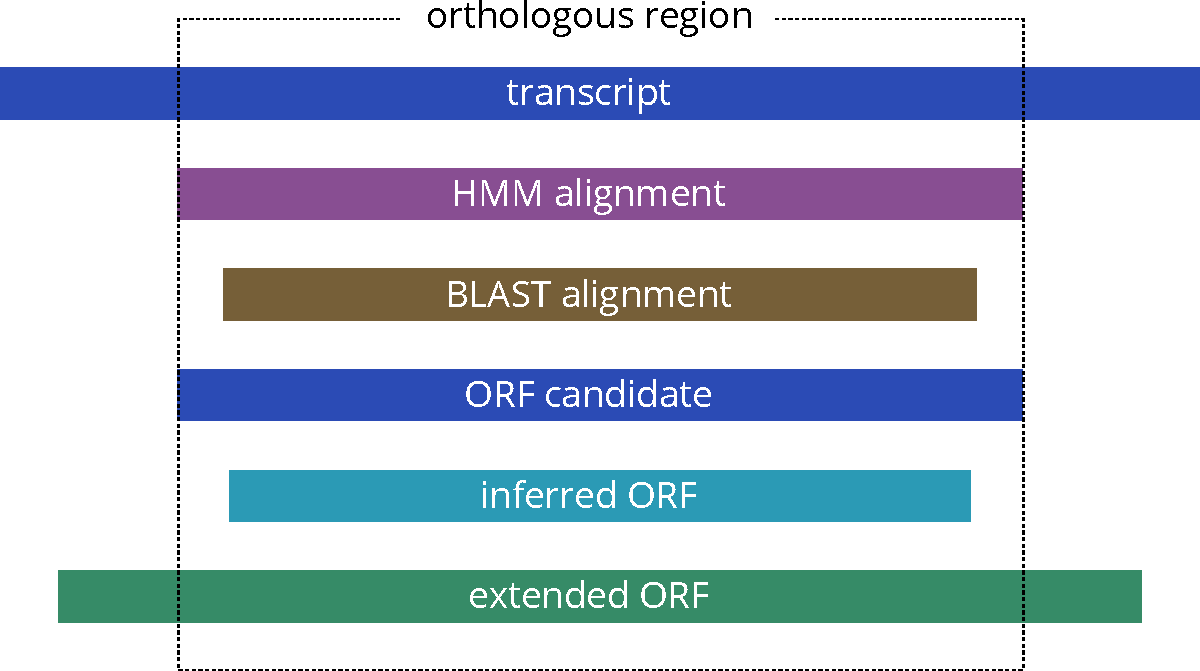
\includegraphics[width=\textwidth]{figures/alignment-regions.pdf}
\caption[Alignment regions in Orthograph]{Alignment regions in
Orthograph. On the transcript, there is a candidate ortholog region that
was identified using a HMM alignment. The reverse search result using
BLAST confirms orthology for the candidate region. For ORF inference,
the transcript subsequence that was identified as putatively orthologous
using the HMM search is used. The resulting ORF may then be extended by
using the entire transcript sequence, resulting in ORF coordinates that
exceed the orthologous region.}
\label{fig:alignment-regions}
\end{figure}

\newpage

\begin{figure}[htbp]
\centering
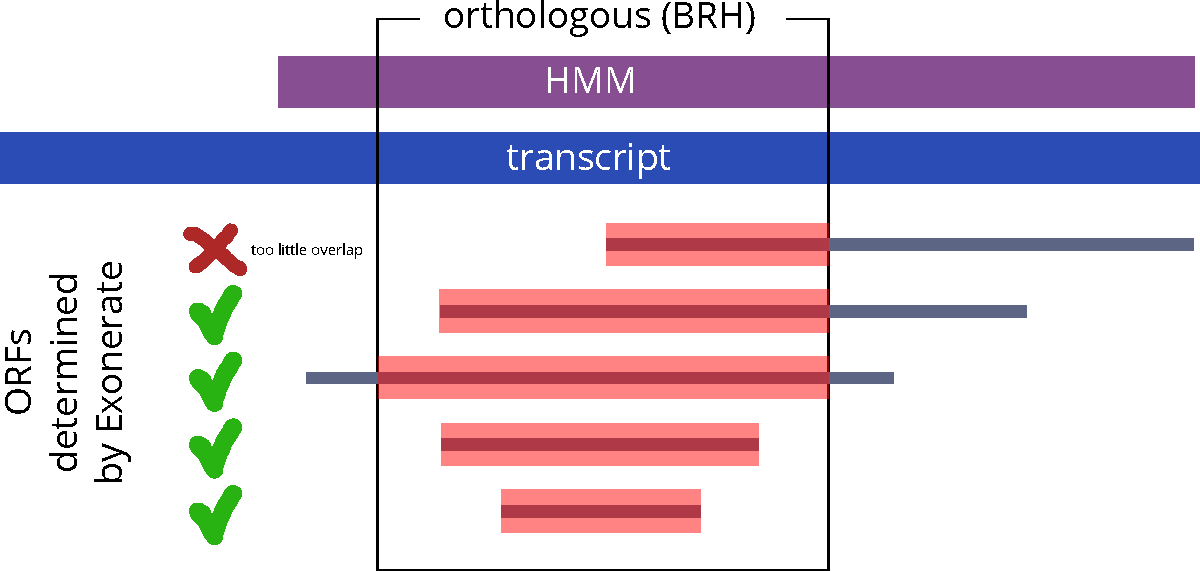
\includegraphics[width=\textwidth]{figures/orf-overlap-minimum.pdf}
\caption[ORF extension criteria in Orthograph]{ORF extension criteria in
Orthograph. Inferred ORFs that do not overlap at least 50 \% of the
orthologous region are discarded due to insufficient confidence in
orthology status. As long as the majority of the ORF length is inside
the orthologous region on the transcript, ORFs are accepted.}
\label{fig:orf-overlap}
\end{figure}

\newpage

\begin{figure}[htbp]
\centering
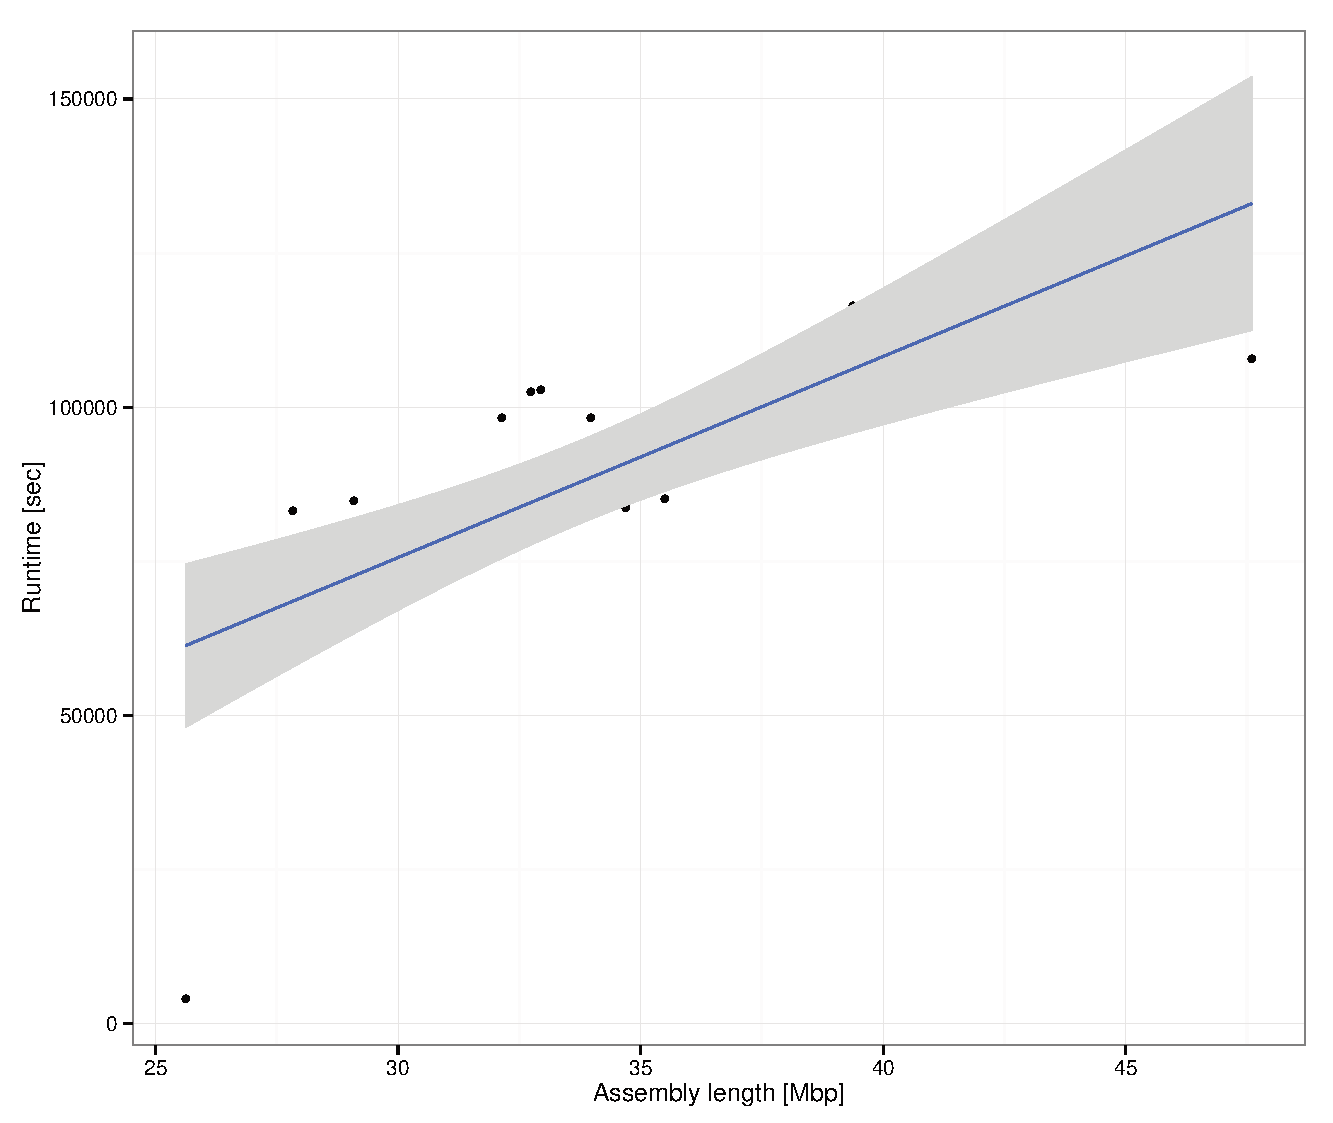
\includegraphics[width=\textwidth]{figures/runtime-vs-length.pdf}
\caption[Orthograph runtime is correlated to assembly length]{Orthograph
runtime is significantly correlated to total transcriptome assembly
length (Spearman rank correlation, $S = 326$, $p \ll 0.001$) when
running with a single thread. Dots indicate measurements for individual
transcriptome assemblies. Blue line: linear regression model; gray area:
confidence interval.}
\label{fig:runtime-vs-length}
\end{figure}

\newpage

\begin{figure}[htbp]
\centering
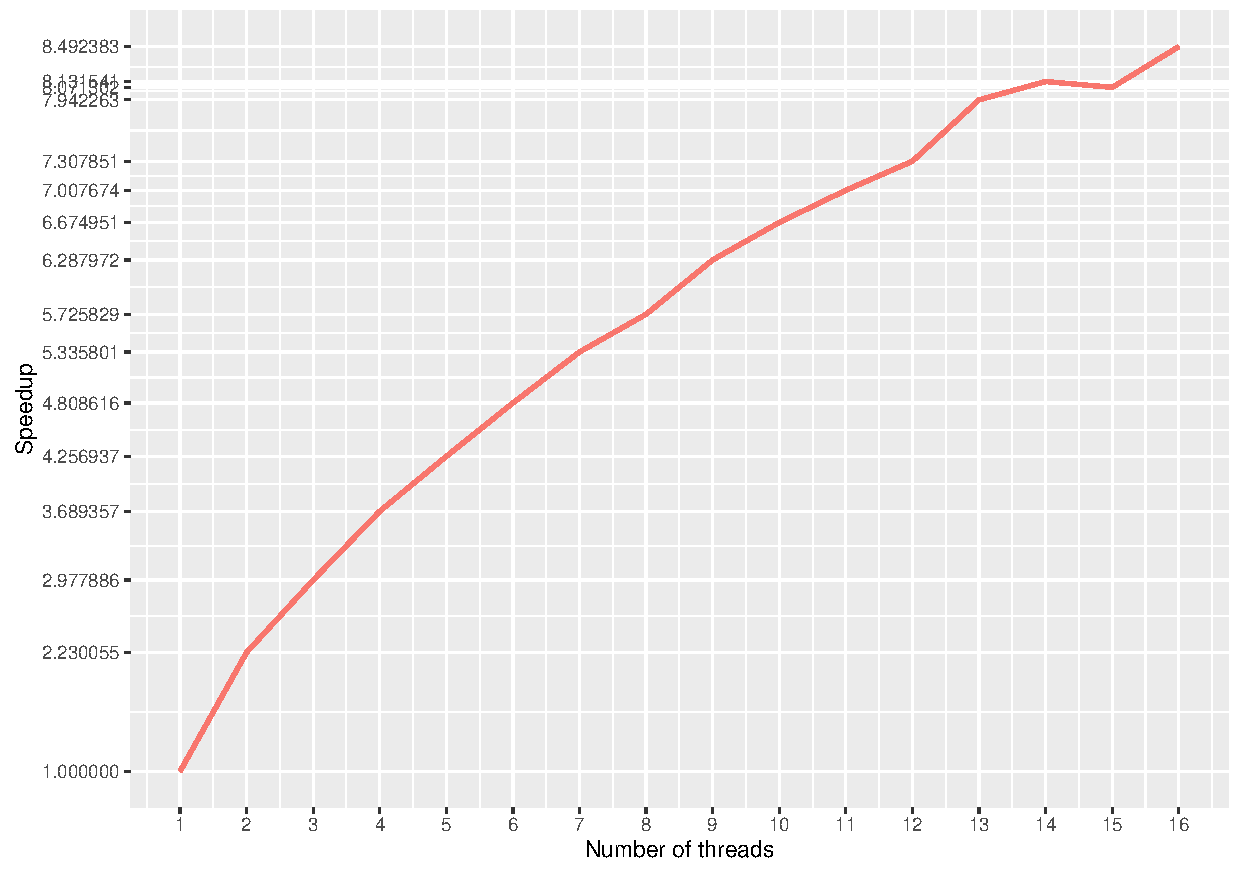
\includegraphics[width=\textwidth]{figures/runtime-speedup.pdf}
\caption[Orthograph multithreading speedup graph]{Orthograph profits
from multiple CPU threads. The x axis shows the number of CPU threads;
the y axis shows the relative speedup compared to single-threaded
performance on a transcriptome assembly of 34 Mbp. Using 16 threads
reduces Orthograph runtime to 11.7 \% of single-threaded runtime.}
\label{fig:runtime-speedup}
\end{figure}

\newpage

\begin{sidewaysfigure}
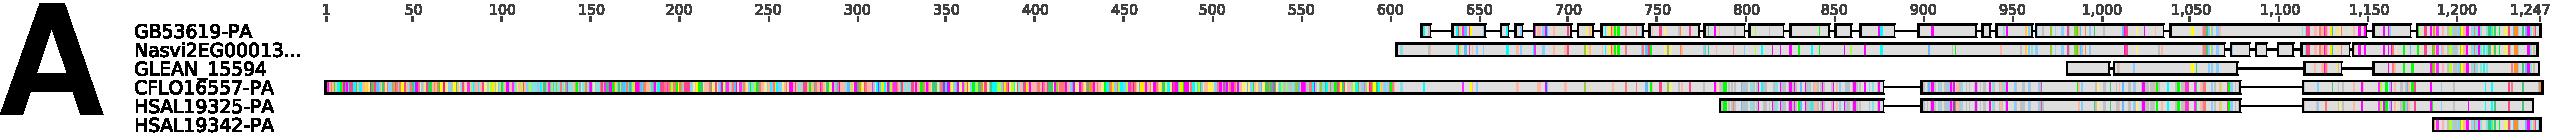
\includegraphics[height=2em]{figures/alignment-clustalw.pdf}\\
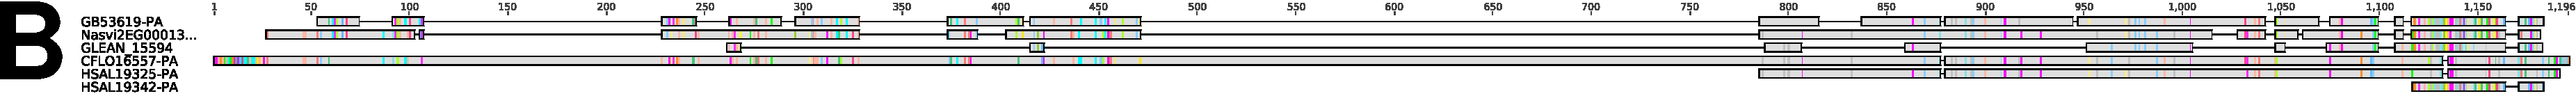
\includegraphics[height=2em]{figures/alignment-muscle.pdf}
\caption[Multiple sequence alignments of an ortholog group]{%
Multiple sequence alignment (MSA) of an ortholog group (OG) as an
examplary assignment of a gene from the \emph{H. saltator} reference
gene set (RGS) to the ``wrong'' OG.  A: Alignment using the ClustalW
algorithm \citep{Thompson1994}; B: Alignment using the MUSCLE algorithm
\citep{Edgar2004}.  According to OrthoDB, the protein HSAL19342-PA
belongs to the OG with the ID EOG7KHN7Q.  Orthograph, however,
identified the protein HSAL19325-PA as orthologous to this OG due to a
high similarity to one of the proteins in the OG (404 amino acids
alignment overlap, 64.6 \% identical sites).  The sequence HSAL19325-PA
has been added to the MSA to demonstrate that it is in large parts more
similar to a sequence from \emph{C. floridanus} (CFLO16557-PA) and
therefore yields a higher alignment bit score than the correct --
according to OrthoDB -- ortholog HSAL19342-PA.  In contrast, the protein
that is recorded in OrthoDB as part of the OG is shorter and displays
little similarity (61 amino acids alignment overlap, 31.1 \% identical
sites).  This leads to a higher bit score in the reverse search for the
longer and more similar -- but not orthologous according to OrthoDB --
sequence.  In turn, the BRH criterion for the correct, but shorter
ortholog (according to OrthoDB) was not fulfilled.  This demonstrates
that using different alignment algorithms can impede successful
orthology assignment.  Grey areas indicate conserved regions, colored
bars indicate sequence-specific different amino acid positions.  Graphic
created using Geneious v7.1 (\url{http://www.geneious.com}).}%
\label{fig:orthodb-alignments}
\end{sidewaysfigure}

\clearpage

\section{Supplementary Tables}

\begin{table}[h]
\footnotesize
\centering
\caption{Species for which 1KITE transcriptomes were analyzed.}
\label{tab:species}
\begin{tabular}{@{}lllll@{}}
\toprule
Order       & Family      & Subfamily      & Genus         & Species                     \\ 
\midrule
Hymenoptera & Crabronidae & Bembicinae     & Alyssontini   & \emph{Alysson spinosus}            \\
Hymenoptera & Crabronidae & Bembicinae     & Bembicini     & \emph{Bembix rostrata}             \\
Hymenoptera & Crabronidae & Bembicinae     & Bembicini     & \emph{Gorytes laticinctus}         \\
Hymenoptera & Crabronidae & Bembicinae     & Bembicini     & \emph{Harpactus elegans}           \\
Hymenoptera & Crabronidae & Bembicinae     & Bembicini     & \emph{Sphecius convallis}          \\
Hymenoptera & Crabronidae & Bembicinae     & Bembicini     & \emph{Stizoides tridentatus}       \\
Hymenoptera & Crabronidae & Bembicinae     & Nyssonini     & \emph{Nysson niger}                \\
Hymenoptera & Crabronidae & Crabroninae    & Crabronini    & \emph{Crabro peltarius}            \\
Hymenoptera & Crabronidae & Crabroninae    & Crabronini    & \emph{Crossocerus quadrimaculatus} \\
Hymenoptera & Crabronidae & Crabroninae    & Larrini       & \emph{Tachysphex fulvitarsis}      \\
Hymenoptera & Crabronidae & Crabroninae    & Oxybelini     & \emph{Oxybelus bipunctatus}        \\
Hymenoptera & Crabronidae & Crabroninae    & Trypoxylini   & \emph{Trypoxylon figulus}          \\
Hymenoptera & Crabronidae & Dinetinae      & -             & \emph{Dinetus pictus}              \\
Hymenoptera & Crabronidae & Pemphredoninae & Pemphredonini & \emph{Diodontus minutus}           \\
Hymenoptera & Crabronidae & Pemphredoninae & Pemphredonini & \emph{Pemphredon lugens}           \\
Hymenoptera & Crabronidae & Pemphredoninae & Psenini       & \emph{Psenulus fuscipennis}        \\
Hymenoptera & Crabronidae & Philanthinae   & Cercerini     & \emph{Cerceris arenaria}           \\
Hymenoptera & Crabronidae & Philanthinae   & Philanthini   & \emph{Philanthus triangulum}       \\
Hymenoptera & Sphecidae   & Ammophilinae   & -             & \emph{Podalonia hirsuta}           \\
Hymenoptera & Sphecidae   & Sceliphrinae   & Sceliphrini   & \emph{Chalybion californicum}      \\
Hymenoptera & Sphecidae   & Sceliphrinae   & Sceliphrini   & \emph{Sceliphron curvatum}         \\
Hymenoptera & Sphecidae   & Sphecinae      & Prionychini   & \emph{Prionyx kirbii}              \\
Hymenoptera & Sphecidae   & Sphecinae      & Sphecini      & \emph{Isodontia mexicana}          \\
Hymenoptera & Sphecidae   & Sphecinae      & Sphecini      & \emph{Sphex funerarius}            \\ 
\bottomrule
\end{tabular}
\end{table}

\begin{table}[h]
\footnotesize
\centering
\caption[Orthograph requirements]{Software packages required by Orthograph. It has been developed and tested with these versions. Older versions are not supported.}
\label{tab:software}
\begin{tabular}{@{}lll@{}}
\toprule
Package     & Version & Download from \\
\midrule
Perl        & 5.14    & \url{http://www.perl.org}                                         \\
SQLite      & 3.8.2   & \url{http://sqlite.org/download.html}                             \\
MySQL       & 5.6.17  & \url{http://dev.mysql.com/downloads/mysql/}                       \\
MAFFT       & 7.023b  & \url{http://mafft.cbrc.jp/alignment/software/}                    \\
HMMer       & 3.1b1   & \url{http://hmmer.janelia.org/software/}                          \\
NCBI BLAST+ & 2.2.28+ & \url{ftp://ftp.ncbi.nlm.nih.gov/blast/executables/blast+/LATEST/} \\
Exonerate   & 2.2.0   & \url{http://www.ebi.ac.uk/~guy/exonerate/}                        \\
\bottomrule
\end{tabular}
\end{table}

\begin{sidewaystable}[h]
\footnotesize
\caption{Official gene sets for the reference ortholog set generation.}
\label{tab:ogs}
\begin{tabular}{@{}llll@{}}
\toprule
Species                         & Version  & Citation \\ \midrule
\species{Acromyrmex echinatior} & 1.2      & \citet{Nygaard2011} \\
\species{Apis mellifera}        & 1.1      & \citet{Honeybee2006} \\
\species{Atta cephalotes}       & 1.2      & \citet{Suen2011} \\
\species{Camponotus floridanus} & 3.3      & \citet{Bonasio2010} \\
\species{Harpegnathos saltator} & 3.3      & \citet{Bonasio2010} \\
\species{Linepithema humile}    & 1.2      & \citet{Smith2011a} \\
\species{Nasonia vitripennis}   & 1.2      & \citet{Werren2010} \\
\species{Tribolium castaneum}   & 3.0      & \citet{TriboliumGenomeSequencingConsortium2008} \\
\bottomrule
\end{tabular}\\
\species{Acromyrmex echinatior}: \url{http://hymenopteragenome.org/acromyrmex/?q=genome_consortium_datasets}\\
\species{Apis mellifera}       : \url{http://hymenopteragenome.org/beebase/?q=download_sequence}\\
\species{Atta cephalotes}      : \url{http://hymenopteragenome.org/atta/?q=genome_consortium_datasets}\\
\species{Camponotus floridanus}: \url{http://hymenopteragenome.org/camponotus/?q=genome_consortium_datasets}\\
\species{Harpegnathos saltator}: \url{http://hymenopteragenome.org/harpegnathos/?q=genome_consortium_datasets}\\
\species{Linepithema humile}   : \url{http://hymenopteragenome.org/linepithema/?q=genome_consortium_datasets}\\
\species{Nasonia vitripennis}  : \url{http://hymenopteragenome.org/nasonia/?q=sequencing_and_analysis_consortium_datasets}\\
\species{Tribolium castaneum}  : \url{http://beetlebase.org/?q=download_settings}
\end{sidewaystable}

% Please add the following required packages to your document preamble:
% \usepackage{booktabs}
\begin{table}[h]
\scriptsize
\caption[Species, 1KITE library IDs, NCBI accession numbers, and assembly
statistics of the apoid wasp transcriptomes that were released with the
Orthograph publication]{Species, 1KITE library IDs (see http:// 1
kite.org/ 1 kite\_species.php ), number of assembled
transcripts, total assembly size, N50 values, and NCBI GenBank accession numbers. Note that the
assemblies were filtered to contain only contigs longer than 199 bp.}
\label{tab:1kite-apoid-wasps-accessions}
\begin{tabular}{@{}lllllll@{}}
\toprule
Species                     & 1KITE library ID   & Tax. ID & BioProject & BioSample accession & Sample acc. & Exp. accession \\ \midrule
\species{Alysson spinosus}            & INSytvTBDRAAPEI-9  & 1507100     & 252289     & SAMN02870203        & SRS651858        & SRX642976            \\
\species{Bembix rostrata}             & INSswpTBNRAAPEI-44 & 1507104     & 252270     & SAMN02870220        & SRS651839        & SRX642957            \\
\species{Cerceris arenaria}           & INSytvTBFRAAPEI-12 & 1507109     & 252291     & SAMN02870235        & SRS651861        & SRX642978            \\
\species{Chalybion californicum}      & INSytvTBQRAAPEI-57 & 411700      & 252298     & SAMN02870236        & SRS651868        & SRX642985            \\
\species{Crabro peltarius}            & INSswpTBJRAAPEI-37 & 1507127     & 252268     & SAMN02870270        & SRS651838        & SRX642955            \\
\species{Crossocerus quadrimaculatus} & INSswpTBPRAAPEI-46 & 1126388     & 252271     & SAMN02870271        & SRS651841        & SRX642958            \\
\species{Dinetus pictus}              & INSjdsTAYRAAPEI-43 & 1507342     & 252320     & SAMN02870280        & SRS651890        & SRX643007            \\
\species{Diodontus minutus}           & INSjdsTBMRAAPEI-88 & 1294192     & 252322     & SAMN02870281        & SRS651892        & SRX643009            \\
\species{Gorytes laticinctus}         & INSytvTBERAAPEI-11 & 1126390     & 252290     & SAMN02870305        & SRS651860        & SRX642977            \\
\species{Harpactus elegans}           & INSswpTAFRAAPEI-16 & 1507137     & 252247     & SAMN02870308        & SRS651818        & SRX642935            \\
\species{Isodontia mexicana}          & INSswpTBDRAAPEI-30 & 288402      & 252264     & SAMN02870321        & SRS651834        & SRX642951            \\
\species{Nysson niger}                & INSswpTBGRAAPEI-34 & 1507151     & 252266     & SAMN02870351        & SRS651836        & SRX642953            \\
\species{Oxybelus bipunctatus}        & INSjdsTBIRAAPEI-75 & 1507154     & 252321     & SAMN02870362        & SRS651891        & SRX643008            \\
\species{Pemphredon lugens}           & INSytvTBBRAAPEI-95 & 1507158     & 252288     & SAMN02870371        & SRS651859        & SRX642975            \\
\species{Philanthus triangulum}       & INSswpTBTRABPEI-62 & 280486      & 252273     & SAMN02870374        & SRS651843        & SRX642960            \\
\species{Podalonia hirsuta}           & INSswpTBRRAAPEI-56 & 1088627     & 252272     & SAMN02870381        & SRS651842        & SRX642959            \\
\species{Prionyx kirbii}              & INSytvTBSRAAPEI-74 & 330847      & 252299     & SAMN02870385        & SRS651869        & SRX642986            \\
\species{Psenulus fuscipennis}        & INSswpTATRAAPEI-13 & 1507163     & 252256     & SAMN02870386        & SRS651827        & SRX642944            \\
\species{Sceliphron curvatum}         & INSswpTAZRAAPEI-19 & 1507168     & 252261     & SAMN02870396        & SRS651832        & SRX642949            \\
\species{Sphecius convallis}          & INSnfrTBORAAPEI-14 & 420963      & 252349     & SAMN02870401        & SRS651919        & SRX643036            \\
\species{Sphex funerarius}            & INSytvTAIRAAPEI-18 & 1507169     & 252279     & SAMN02870403        & SRS651849        & SRX642966            \\
\species{Stizoides tridentatus}       & INSytvTARRAAPEI-44 & 1507174     & 252284     & SAMN02870412        & SRS651854        & SRX642971            \\
\species{Tachysphex fulvitarsis}      & INSswpTAKRAAPEI-21 & 1507176     & 252251     & SAMN02870419        & SRS651822        & SRX642939            \\
\species{Trypoxylon figulus}          & INSytvTAWRAAPEI-88 & 1124897     & 252286     & SAMN02870436        & SRS651856        & SRX642973            \\ \bottomrule
\end{tabular}

\bigskip

\begin{tabular}{@{}lllllll@{}}
\toprule
Species                     & Run accession & TSA project accession & TSA version  & Transcripts & Total length & N50   \\ \midrule
\species{Alysson spinosus}            & SRR1503092    & GBUA00000000          & GBUA01000000 & 40,680      & 47,606,733   & 1,568 \\
\species{Bembix rostrata}             & SRR1503073    & GBQR00000000          & GBQR01000000 & 33,341      & 37,839,804   & 6,031 \\
\species{Cerceris arenaria}           & SRR1503094    & GBNS00000000          & GBNS01000000 & 24,719      & 34,252,864   & 3,305 \\
\species{Chalybion californicum}      & SRR1503101    & GBOM00000000          & GBOM01000000 & 21,323      & 33,977,878   & 3,834 \\
\species{Crabro peltarius}            & SRR1503071    & GBWG00000000          & GBWG01000000 & 17,826      & 27,839,732   & 4,932 \\
\species{Crossocerus quadrimaculatus} & SRR1503074    & GBWH00000000          & GBWH01000000 & 16,354      & 27,670,170   & 5,280 \\
\species{Dinetus pictus}              & SRR1503123    & GBLS00000000          & GBLS01000000 & 20,195      & 35,261,360   & 5,479 \\
\species{Diodontus minutus}           & SRR1503125    & GBMA00000000          & GBMA01000000 & 22,820      & 39,373,028   & 3,107 \\
\species{Gorytes laticinctus}         & SRR1503093    & GBNR00000000          & GBNR01000000 & 20,336      & 30,119,789   & 7,540 \\
\species{Harpactus elegans}           & SRR1503051    & GBNF00000000          & GBNF01000000 & 22,245      & 35,499,888   & 4,814 \\
\species{Isodontia mexicana}          & SRR1503067    & GBPY00000000          & GBPY01000000 & 34,622      & 38,000,489   & 2,600 \\
\species{Nysson niger}                & SRR1503069    & GBNN00000000          & GBNN01000000 & 22,496      & 29,091,955   & 4,151 \\
\species{Oxybelus bipunctatus}        & SRR1503124    & GBLU00000000          & GBLU01000000 & 22,233      & 37,187,137   & 2,311 \\
\species{Pemphredon lugens}           & SRR1503091    & GBQH00000000          & GBQH01000000 & 24,675      & 39,425,911   & 716   \\
\species{Philanthus triangulum}       & SRR1503076    & GBWI00000000          & GBWI01000000 & 21,735      & 27,360,360   & 4,209 \\
\species{Podalonia hirsuta}           & SRR1503075    & GBPX00000000          & GBPX01000000 & 21,108      & 32,136,789   & 4,075 \\
\species{Prionyx kirbii}              & SRR1503102    & GBQI00000000          & GBQI01000000 & 21,703      & 31,095,319   & 8,540 \\
\species{Psenulus fuscipennis}        & SRR1503060    & GBNH00000000          & GBNH01000000 & 24,423      & 31,095,907   & 1,024 \\
\species{Sceliphron curvatum}         & SRR1503065    & GBNL00000000          & GBNL01000000 & 22,934      & 32,739,311   & 6,440 \\
\species{Sphecius convallis}          & SRR1503152    & GBOB00000000          & GBOB01000000 & 19,967      & 25,618,375   & 3,922 \\
\species{Sphex funerarius}            & SRR1503082    & GBQD00000000          & GBQD01000000 & 26,189      & 37,503,328   & 1,476 \\
\species{Stizoides tridentatus}       & SRR1503087    & GBQO00000000          & GBQO01000000 & 27,724      & 34,689,230   & 5,790 \\
\species{Tachysphex fulvitarsis}      & SRR1503055    & GBPR00000000          & GBPR01000000 & 17,308      & 32,940,922   & 8,852 \\
\species{Trypoxylon figulus}          & SRR1503089    & GBWO00000000          & GBWO01000000 & 19,174      & 31,640,527   & 4,800 \\ \bottomrule
\end{tabular}
\end{table}

\newpage

\addcontentsline{toc}{section}{References}
\bibliographystyle{apalike2}
\bibliography{references}

\end{appendices}

\backmatter

\end{document}
